%%%%%%%%%%%%%%%%%%%%%%%%%%%%%%%%%%%%%%%%%%%%%%%%%%%%%%%%%%%%%%%%%%%%%%%%%%%%%%%%%

%%%%%%%%%%%%%%%%%%%%%%%%%%%%%%%%%%%%%%%%%%%%%%%%%%%%%%%%%%%%%%%%%%%%%%%%%%%%%%%%%
%% Documenclass 
%%%%%%%%%%%%%%%%%%%%%%%%%%%%%%%%%%%%%%%%%%%%%%%%%%%%%%%%%%%%%%%%%%%%%%%%%%%%%%%%%
\documentclass[a4paper,oneside,titlepage,12pt]{report}
%%%%%%%%%%%%%%%%%%%%%%%%%%%%%%%%%%%%%%%%%%%%%%%%%%%%%%%%%%%%%%%%%%%%%%%%%%%%%%%%%
%% Packages
%%%%%%%%%%%%%%%%%%%%%%%%%%%%%%%%%%%%%%%%%%%%%%%%%%%%%%%%%%%%%%%%%%%%%%%%%%%%%%%%%
\usepackage[spanish]{babel}
\usepackage{multirow}
\usepackage{amsmath}
\usepackage{complexity}
\usepackage[T1]{fontenc}
\usepackage[utf8]{inputenc}
\usepackage[pdftex]{graphicx} %%Graphics in pdfLaTeX
\usepackage{csquotes}
\usepackage{a4wide} %%Smaller margins, more text per page.
\usepackage{longtable} %%For tables that exceed a page width
\usepackage{pdflscape} %%Adds PDF sup­port to the land­scape en­vi­ron­ment of pack­age
\usepackage{caption} %%Pro­vides many ways to cus­tomise the cap­tions in float­ing en­vi­ron­ments like fig­ure and ta­ble
\usepackage{float} %%Im­proves the in­ter­face for defin­ing float­ing ob­jects such as fig­ures and ta­bles
\usepackage[tablegrid,nochapter]{vhistory} %%Vhis­tory sim­pli­fies the cre­ation of a his­tory of ver­sions of a doc­u­ment
\usepackage[nottoc]{tocbibind} %%Au­to­mat­i­cally adds the bib­li­og­ra­phy and/or the in­dex and/or the con­tents, etc., to the Ta­ble of Con­tents list­ing
\usepackage[toc,page]{appendix} %%The ap­pendix pack­age pro­vides var­i­ous ways of for­mat­ting the ti­tles of ap­pen­dices
\usepackage{pdfpages} %%This pack­age sim­pli­fies the in­clu­sion of ex­ter­nal multi-page PDF doc­u­ments in LATEX doc­u­ments
\usepackage[rightcaption]{sidecap} %%De­fines en­vi­ron­ments called SC­fig­ure and SCtable (anal­o­gous to fig­ure and ta­ble) to type­set cap­tions side­ways
% \usepackage{cite} %%The pack­age sup­ports com­pressed, sorted lists of nu­mer­i­cal ci­ta­tions, and also deals with var­i­ous punc­tu­a­tion and other is­sues of rep­re­sen­ta­tion, in­clud­ing com­pre­hen­sive man­age­ment of break points
\usepackage[printonlyused]{acronym} %%This pack­age en­sures that all acronyms used in the text are spelled out in full at least once. It also pro­vides an en­vi­ron­ment to build a list of acronyms used
\usepackage[pdftex,scale={.8,.8}]{geometry} %%The pack­age pro­vides an easy and flex­i­ble user in­ter­face to cus­tomize page lay­out, im­ple­ment­ing auto-cen­ter­ing and auto-bal­anc­ing mech­a­nisms so that the users have only to give the least de­scrip­tion for the page lay­out. For ex­am­ple, if you want to set each mar­gin 2cm with­out header space, what you need is just \usep­a­ck­age[mar­gin=2cm,no­head]{ge­om­e­try}.
\usepackage{layout} %%The pack­age de­fines a com­mand \lay­out, which will show a sum­mary of the lay­out of the cur­rent doc­u­ment
\usepackage{subfigure} %%Pro­vides sup­port for the ma­nip­u­la­tion and ref­er­ence of small or ‘sub’ fig­ures and ta­bles within a sin­gle fig­ure or ta­ble en­vi­ron­ment.
\usepackage[toc]{glossaries} %%The glos­saries pack­age sup­ports acronyms and mul­ti­ple glos­saries, and has pro­vi­sion for op­er­a­tion in sev­eral lan­guages (us­ing the fa­cil­i­ties of ei­ther ba­bel or poly­glos­sia).
\usepackage[left,pagewise,modulo]{lineno} %%Adds line num­bers to se­lected para­graphs with ref­er­ence pos­si­ble through the LATEX \ref and \pageref cross ref­er­ence mech­a­nism
\usepackage[pdftex,colorlinks=false,hidelinks,pdfstartview=FitV,bookmarks=true]{hyperref}%%The hy­per­ref pack­age is used to han­dle cross-ref­er­enc­ing com­mands in LATEX to pro­duce hy­per­text links in the doc­u­ment. 
\usepackage{metainfo}
\usepackage[pagestyles,raggedright]{titlesec}
\usepackage{etoolbox}
\usepackage{tabularx}
\usepackage{ltxtable}
\usepackage[style=ieee]{biblatex}
\bibliography{base/sources.bib}
\usepackage[nottoc]{tocbibind}
\usepackage[official]{eurosym}
\usepackage{gensymb}
\usepackage{%
	array, %%An ex­tended im­ple­men­ta­tion of the ar­ray and tab­u­lar en­vi­ron­ments which ex­tends the op­tions for col­umn for­mats, and pro­vides "pro­grammable" for­mat spec­i­fi­ca­tions
	booktabs, %%The pack­age en­hances the qual­ity of ta­bles in LATEX, pro­vid­ing ex­tra com­mands as well as be­hind-the-scenes op­ti­mi­sa­tion
	dcolumn, %%
	rotating,
	shortvrb,
	units,
	url,
	lastpage,
	longtable,
	lscape,
	qtree,
	skmath,	
	enumitem,
}
%%%%%%%%%%%%%%%%%%%%%%%%%%%%%%%%%%%%%%%%%%%%%%%%%%%%%%%%%%%%%%%%%%%%%%%%%%%%%%%%%
%% Java --> latex 
%%%%%%%%%%%%%%%%%%%%%%%%%%%%%%%%%%%%%%%%%%%%%%%%%%%%%%%%%%%%%%%%%%%%%%%%%%%%%%%%%
\usepackage{listings}

\lstset{ %
  backgroundcolor=\color{white},   % Indica el color de fondo; necesita que se añada \usepackage{color} o \usepackage{xcolor}
  basicstyle=\footnotesize\ttfamily,        % Fija el tamaño del tipo de letra utilizado para el código
  breakatwhitespace=false,         % Activarlo para que los saltos automáticos solo se apliquen en los espacios en blanco
  inputencoding=utf8,
  breaklines=true,                 % Activa el salto de línea automático
  captionpos=b,                    % Establece la posición de la leyenda del cuadro de código
  commentstyle=\color{darkgreen},    % Estilo de los comentarios
  extendedchars=true,              % Permite utilizar caracteres extendidos no-ASCII; solo funciona para codificaciones de 8-bits; para UTF-8 no funciona. En xelatex necesita estar a true para que funcione.
  frame=single,	                   % Añade un marco al código
  keepspaces=true,                 % Mantiene los espacios en el texto. Es útil para mantener la indentación del código(puede necesitar columns=flexible).
  columns=flexible,
  keywordstyle=\color{darkorange},       % estilo de las palabras clave
  language=C,                 % El lenguaje del código
  otherkeywords={__attribute__, __interrupt__, config, inline, asm, uint8_t, uint16_t,%
  uint32_t, uint64_t, time_t, size_t, Servo, Motor, Nop},           % Si se quieren añadir otras palabras clave al lenguaje
  numbers=left,                    % Posición de los números de línea (none, left, right).
  numbersep=5pt,                   % Distancia de los números de línea al código
  numberstyle=\small\color{gray}, % Estilo para los números de línea
  rulecolor=\color{black},         % Si no se activa, el color del marco puede cambiar en los saltos de línea entre textos que sea de otro color, por ejemplo, los comentarios, que están en verde en este ejemplo
  showspaces=false,                % Si se activa, muestra los espacios con guiones bajos; sustituye a 'showstringspaces'
  showstringspaces=false,          % subraya solamente los espacios que estén en una cadena de esto
  showtabs=false,                  % muestra las tabulaciones que existan en cadenas de texto con guión bajo
  stringstyle=\color{darkgreen},     % Estilo de las cadenas de texto
  identifierstyle=\color{blue},
  tabsize=4,	                   % Establece el salto de las tabulaciones a 2 espacios
  title=\lstname,                   % muestra el nombre de los ficheros incluidos al utilizar
  caption=\lstname,
  literate={á}{{\'a}}1 {é}{{\'e}}1 {í}{{\'{\i}}}1 {ó}{{\'o}}1 {ú}{{\'u}}1 {Á}{{\'A}}1 {É}{{\'E}}1 {Í}{{\'I}}1 {Ó}{{\'O}}1 {Ú}{{\'U}}1 {ü}{{\"u}}1 {Ü}{{\"U}}1 {ñ}{{\~n}}1 {Ñ}{{\~N}}1 {¿}{{?``}}1 {¡}{{!``}}1 {º}{\textdegree}1
}

\usepackage{xcolor}
\definecolor{pblue}{rgb}{0.13,0.13,1}
\definecolor{pgreen}{rgb}{0,0.5,0}
\definecolor{pred}{rgb}{0.9,0,0}
\definecolor{pgrey}{rgb}{0.46,0.45,0.48}
\definecolor{darkgreen}{rgb}{0.0, 0.4, 0.0}
\definecolor{darkorange}{rgb}{1.0, 0.55, 0.0}
\usepackage{inconsolata}
%%%%%%%%%%%%%%%%%%%%%%%%%%%%%%%%%%%%%%%%%%%%%%%%%%%%%%%%%%%%%%%%%%%%%%%%%%%%%%%%%
\setlength{\parindent}{0pt}
\setlength{\parskip}{.5\baselineskip}
%%%%%%%%%%%%%%%%%%%%%%%%%%%%%%%%%%%%%%%%%%%%%%%%%%%%%%%%%%%%%%%%%%%%%%%%%%%%%%%%%
%% Inserting the metadata
%%%%%%%%%%%%%%%%%%%%%%%%%%%%%%%%%%%%%%%%%%%%%%%%%%%%%%%%%%%%%%%%%%%%%%%%%%%%%%%%%
% % Metadaten des Dokumentes

\def\Company{Consultancy}
\def\Institute{\textit{Universidad Politécnica de Madrid}}
\def\Course{\textit{Ingeniería de Computadores}}
\def\Module{\textit{Trabajo de Fin de Grado}}
\def\Docent{\textit{Tutor: Norberto Cañas de Paz} \\ \textit{Marina Pérez Giménez}}
\def\Assistant{}

\def\BoldTitle{Memoria del proyecto}

\def\Subtitle{para el \\ Trabajo de Fin de Grado sobre el manipulador \pArm{} \\}
\def\Authors{Javier Alonso Silva \\ Mihai Octavian Stanescu \\ José Alejandro Moya Blanco } 
\def\Shortname{J. Alonso, M. Stanescu, A. Moya}


\title{\textbf{\BoldTitle}\\\Subtitle}
\author{\Authors \\ \\ \\ \Institute\\ \Course\\ \Module\\ \\ \Docent}
\date{Madrid, \today{}}

%%%%%%%%%%%%%%%%%%%%%%%%%%%%%%%%%%%%%%%%%%%%%%%%%%%%%%%%%%%%%%%%%%%%%%%%%%%%%%%%%
%% Creation of pdf information
%%%%%%%%%%%%%%%%%%%%%%%%%%%%%%%%%%%%%%%%%%%%%%%%%%%%%%%%%%%%%%%%%%%%%%%%%%%%%%%%%
\hypersetup{pdfinfo={
		Title={Title},
		Author={TR},
		Subject={Report}
	}}
%%%%%%%%%%%%%%%%%%%%%%%%%%%%%%%%%%%%%%%%%%%%%%%%%%%%%%%%%%%%%%%%%%%%%%%%%%%%%%%%%
%% Creating the frontpage
%%%%%%%%%%%%%%%%%%%%%%%%%%%%%%%%%%%%%%%%%%%%%%%%%%%%%%%%%%%%%%%%%%%%%%%%%%%%%%%%%
\AtBeginDocument{
	\maketitle
	\thispagestyle{empty}
}

%%%%%%%%%%%%%%%%%%%%%%%%%%%%%%%%%%%%%%%%%%%%%%%%%%%%%%%%%%%%%%%%%%%%%%%%%%%%%%%%%
%% Creation of the header
%%%%%%%%%%%%%%%%%%%%%%%%%%%%%%%%%%%%%%%%%%%%%%%%%%%%%%%%%%%%%%%%%%%%%%%%%%%%%%%%%
\patchcmd{\chapter}{plain}{short}{}{} %$ <-- the header on chapter 1
%%%%%%%%%%%%%%%%%%%%%%%%%%%%%%%%%%%%%%%%%%%%%%%%%%%%%%%%%%%%%%%%%%%%%%%%%%%%%%%%%
%% Creation of page-styles
%%%%%%%%%%%%%%%%%%%%%%%%%%%%%%%%%%%%%%%%%%%%%%%%%%%%%%%%%%%%%%%%%%%%%%%%%%%%%%%%%
\newpagestyle{long}{%
	\sethead[\thepage][][\chaptername\ \thechapter:\ \chaptertitle]{\chaptername\ \thechapter:\ \chaptertitle}{}{\thepage}
	\headrule
}

\newpagestyle{short}{%
	\sethead[\thepage][][]{}{}{\thepage}
	\headrule
}

% % workaround
% \makeatletter
% \appto{\appendices}{\def\Hy@chapapp{Appendix}}
% \makeatother

\addto\captionsspanish{%
  \renewcommand\appendixname{Anexo}
  \renewcommand\appendixpagename{Anexos}
}

\newcommand{\pArm}{\textit{p}Arm}

\newcolumntype{s}{>{\hsize=.5\hsize\linewidth=\hsize}X}
\newcolumntype{b}{>{\hsize=.75\hsize}X}
\newcommand{\heading}[1]{\multicolumn{1}{c}{#1}}

\newcolumntype{L}[1]{>{\hsize=#1\hsize\raggedright\arraybackslash}X}%
\newcolumntype{R}[1]{>{\hsize=#1\hsize\raggedleft\arraybackslash}X}%
\newcolumntype{C}[1]{>{\hsize=#1\hsize\centering\arraybackslash}X}%

%%%%%%%%%%%%%%%%%%%%%%%%%%%%%%%%%%%%%%%%%%%%%%%%%%%%%%%%%%%%%%%%%%%%%%%%%%%%%%%%%
%% DOCUMENT
%%%%%%%%%%%%%%%%%%%%%%%%%%%%%%%%%%%%%%%%%%%%%%%%%%%%%%%%%%%%%%%%%%%%%%%%%%%%%%%%%

\begin{document}

\renewcommand{\tablename}{Tabla}

\pagenumbering{roman}
\DeclareGraphicsExtensions{.pdf,.jpg,.png}
\pagestyle{short}

\newpage
%%%%%%%%%%%%%%%%%%%%%%%%%%%%%%%%%%%%%%%%%%%%%%%%%%%%%%%%%%%%%%%%%%%%%%%%%%%%%%%%%
%% Table of contents
%%%%%%%%%%%%%%%%%%%%%%%%%%%%%%%%%%%%%%%%%%%%%%%%%%%%%%%%%%%%%%%%%%%%%%%%%%%%%%%%%
\tableofcontents
\listoffigures
\listoftables

\newpage
\pagestyle{long}


%%%%%%%%%%%%%%%%%%%%%%%%%%%%%%%%%%%%%%%%%%%%%%%%%%%%%%%%%%%%%%%%%%%%%%%%%%%%%%%%%
%% Version table insertion
%%%%%%%%%%%%%%%%%%%%%%%%%%%%%%%%%%%%%%%%%%%%%%%%%%%%%%%%%%%%%%%%%%%%%%%%%%%%%%%%%
% Versionstabelle.

\chapter*{Historial de versiones}
\addcontentsline{toc}{chapter}{Historial de versiones}

% \renewcommand{\vhhistoryname}{Revisión}
% \renewcommand{\vhchangename}{Descripción}
% \renewcommand{\vhversionname}{Versión}
% \renewcommand{\vhdatename}{Fecha}
% \renewcommand{\vhauthorname}{Autor(es)}

\begin{table}[H]
    \centering
    \begin{tabularx}{\textwidth}{| c | l | l | X |}
        \hline
        \textbf{Revisión} & \textbf{Fecha} & \textbf{Autor(es)} & \textbf{Descripción} \\
        \hline
        000 & 27.05.2020 & \Shortname & Comienzo del desarrollo de la memoria. \\
        \hline
        001 & 16.06.2020 & \Shortname & Primera revisión de la memoria -- revisados los puntos 1.1 y 2 \\
        \hline
        002 & 23.06.2020 & \Shortname & Revisados los puntos 5.1, 5.2, 5.3 \\
        \hline
        003 & 30.06.2020 & \Shortname & Revisados los puntos 1.2, 1.3 y 3.1 \\
        \hline
    \end{tabularx}
    \label{tab:hrevision}
\end{table}

% \begin{versionhistory}
% 	\vhEntry{1.0}{25.01.2020}{\Shortname}{Primera especificación}
% \end{versionhistory}

\chapter*{Definiciones, siglas, y abreviaturas}
\begin{acronym}
    \acro{SDK}{\textit{Software Development Kit}}
    \acro{ROS}{\textit{Robot Operating System}}
    \acro{API}{\textit{Application Programming Interface}}
    \acro{SW}{\textit{software}}
    \acro{HW}{\textit{hardware}}
    \acro{pArm}{\textit{Printed -- Arm}}
    \acro{USB}{\textit{Universal Serial Bus}}
    \acro{ODS}{Objetivos de Desarrollo Sostenible}
    \acro{OS}{\textit{Open--Source}}
    \acro{OH}{\textit{Open--Hardware}}
    \acro{S1}{Sistema 1 -- ordenador}
    \acro{S2}{Sistema 2 -- \pArm{}}
    \acro{GUI}{\textit{Graphical User Interface}}
    \acro{GTK}{\textit{GIMP Toolkit}}
    \acro{SoC}{\textit{System On Chip}}
    \acro{PWM}{\textit{Pulse--Width Modulation}}
    \acro{GPIO}{\textit{General Purpose Input/Output}}
    \acro{UART}{\textit{Universal Asynchronous Receiver--Transmitter}}
    \acro{RAM}{\textit{Random Access Memory}}
    \acro{ADC}{\textit{Analog--Digital Conversor}}
    \acro{PLA}{Ácido Poliláctico}
    \acro{ABS}{Acrilonitrilo Butadieno Estireno}
    \acro{DSP}{\textit{Digital Signal Processor}}
    \acro{PLL}{\textit{Phase Loop Lock}}
    \acro{THT}{\textit{Through-Hole Technology}}
    \acro{SMD}{\textit{surface-mount device}}
    \acro{PCB}{\texit{Printed circuit board}}
    
\end{acronym}

\begin{itemize}
    \item \ac{SDK} -- colección de herramientas \ac{SW} disponibles para instalar en un único paquete.
    \item \textit{hand--shake} -- en informática, negociación entre pares para establecer de forma dinámica los parámetros de un canal de comunicaciones. 
    \item \ac{ROS} -- conjunto de librerías \ac{SW} que ayudan a construir aplicaciones para robots.
    \item \textit{Firmware} -- \ac{SW} programado que especifica el orden de ejecución del sistema.
    \item \ac{GUI} -- siglas que significan ``Interfaz Gráfica de Usuario'' (en castellano).
    \item \ac{GTK} -- biblioteca de componentes gráficos multiplataforma para desarrollar interfaces gráficas de usuario.
    \item \ac{SoC} -- tecnología de fabricación que integra todos o gran parte de los módulos en un circuito integrado. 
    \item \ac{PWM} -- Señal cuadrada de periodo habitualmente constante, entre flancos de subida, en la que se modula el tiempo a nivel alto
    \item \ac{GPIO} -- pin genérico cuyo comportamiento puede ser controlado en tiempo de ejecución.
    \item \ac{UART} -- estándar de comunicación dúplex.
    \item Dúplex -- término que define a un sistema que es capaz de mantener una comunicación bidireccional, enviando y recibiendo mensajes de forma simultánea.
    \item Widget -- la parte de una GUI (interfaz gráfica de usuario) que permite al usuario interconectar con la aplicación.
    \item \ac{RAM} -- memoria principal del ordenador, donde se guardan programas y datos, sobre la que se pueden efectuar operaciones de lectura y escritura.
    \item \textit{Deep--Sleep} -- estado de un microcontrolador en el cual consume muy poca cantidad de energía.
    \item \textit{bit} -- unidad mínima de información de un computador digital.
    \item \ac{THT} -- tecnología que utiliza agujeros pasantes que se practican en las placas de los circuitos impresos para el montaje de diferentes elementos electrónicos.
    \item \ac{SMD} -- tecnología que utiliza componentes de montaje superficial para la inserción de diferentes elementos electrónicos en un circuito impreso.
    \item \ac{PCB} -- Placa de circuito impreso.
\end{itemize}

\addcontentsline{toc}{chapter}{Definiciones, siglas, y abreviatura}
\newpage
\pagenumbering{arabic}
%%%%%%%%%%%%%%%%%%%%%%%%%%%%%%%%%%%%%%%%%%%%%%%%%%%%%%%%%%%%%%%%%%%%%%%%%%%%%%%%%
%% Inserting all the content
%%%%%%%%%%%%%%%%%%%%%%%%%%%%%%%%%%%%%%%%%%%%%%%%%%%%%%%%%%%%%%%%%%%%%%%%%%%%%%%%%
\chapter{Motivación y objetivos}
%% REVISADO
\section{Estado del arte}
\subsection{Desarrollo de la robótica a lo largo de la historia}

El mundo de la robótica da acceso a resolver una gran variedad de problemas donde el ser humano estaba
limitado físicamente: levantar cargas de gran peso, realizar tareas repetitivas durante tiempos
prolongados, etc. Además, como bien se sabe, ha permitido el desarrollo de cadenas de producción en
masa para poder desarrollar y crear los productos que usamos diariamente, desde el coche hasta el 
teléfono móvil.

Desde que se empezó a investigar en este campo, el desarrollo de los brazos robóticos ha sido 
exponencial: se empezó trabajando con pequeños autómatas hasta el desarrollo de la revolución
industrial \cite{moran_evolution_2007}.

Los primeros modelos, como se puede ver en la figura \ref{fig:evolution}, empezaron intentando hacer
representaciones de las manos humanas. En particular, se crearon un flautista y un tamborilero los
cuales eran capaces de tocar los respectivos instrumentos utilizando un complejo sistema de cables y 
engranajes para poder mover los ``dedos'' de los músicos.

\begin{figure}[H]
    \centering
    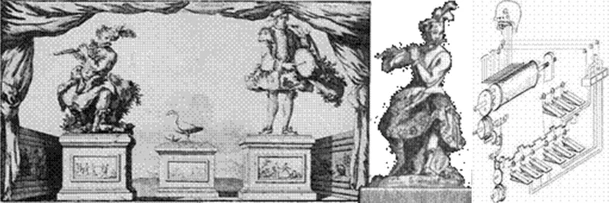
\includegraphics[width=.75\linewidth]{pictures/evolution_of_robotic_arms.png}
    \caption{Flautista y tamborilero de Vaucanson \cite{vaucanson_mecanisme_1738}.}
    \label{fig:evolution}
\end{figure}

Siguiendo con esta idea, se fue mejorando y desarrollando el modelo de imitación de las articulaciones
y los miembros de los humanos, llegando a construir estructuras más complejas y avanzadas, pensadas en 
su momento para poder tocar el clavicordio mediante un muñeco, como se muestra en la figura 
\ref{fig:lady_musician}:

\begin{figure}[H]
    \centering
    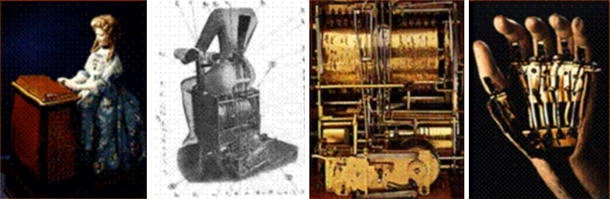
\includegraphics[width=.8\linewidth]{pictures/reproduction_of_lady_musician.png}
    \caption{En 1774, ``lady musician'' por Jaquet-Droz \cite{chapuis_alfred_and_droz_edmond_automata_1958}.}
    \label{fig:lady_musician}
\end{figure}

Durante los años siguientes, el proceso se fue refinando hasta el punto de desarrollar un autómata
el cual era capaz de jugar al ajedrez, llamado ``The Turk'' \cite{standage_tom_turk_2002}, construido
en 1769. La estructura comprendía un conjunto de mecanismos los cuales eran controlados por un operador,
encargado de realizar los movimientos del brazo izquierdo del autómata.

En la figura \ref{fig:turk} se puede ver cómo está diseñado el sistema para mover un controlador 
pantográfico sobre el tablero de juego, controlado por el operador externo antes mencionado:

\begin{figure}[H]
    \centering
    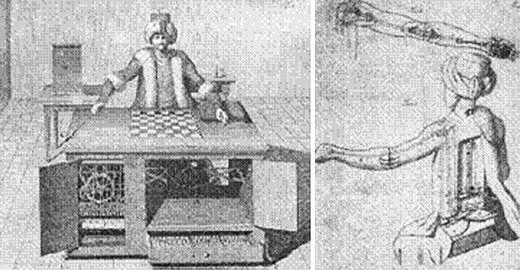
\includegraphics[width=.75\linewidth]{pictures/chess_evolution.png}
    \caption{``The Turk'', creado por von Kempelen en 1769 \cite{standage_tom_turk_2002}.}
    \label{fig:turk}
\end{figure}

Desde entonces, la robótica ha evolucionado y crecido de manera exponencial. Por una parte, debidas
las distintas guerras que han habido en los últimos 200 años, se ha dado un gran impulso a la 
industria encargada de crear distintos dispositivos con fines de defensa y ataque. En particular,
se potenciaron mucho los desarrollos de dispositivos por control remoto, destacando el diseño de
NiKola Tesla en 1898 de un barco completamente automatizado, controlado por control remoto y sumergible,
como se puede ver en la figura \ref{fig:nicola_tesla_boat}:

\begin{figure}[H]
    \centering
    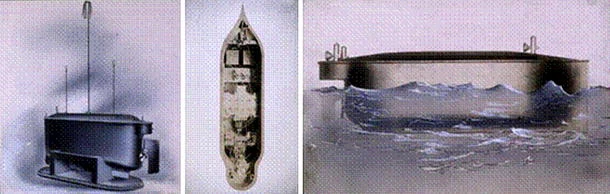
\includegraphics[width=.75\linewidth]{pictures/nicola_tesla_boat.png}
    \caption{Barco a control remoto de Nicola Tesla, en 1898 \cite{belarmino_j_and_moran_me_and_firoozi_f_and_capello_s_and_kolios_e_and_perrotti_m_teslas_2005}.}
    \label{fig:nicola_tesla_boat}
\end{figure}

Por otro lado, dada la cantidad de bajas de las Primera y Segunda Guerras Mundiales, se empezaron a
desarrollar robots que permitieran sustituir a los militares en el campo de batalla, destacando en este
campo el robot ``Elektro'', creado por la compañía Westinghouse. Dicho robot supuso un gran éxito en la
industria de los robots y armamentística, pudiendo moverse completamente, disparar armas, mover elementos
faciales para ``expresar emociones'' e inclusive poder comunicarse.

En la figura \ref{fig:elektro}, se puede ver a la izquierda la primera versión ``Alpha'' y, a la derecha,
la versión mejorada ``Elektro'':

\begin{figure}[H]
    \centering
    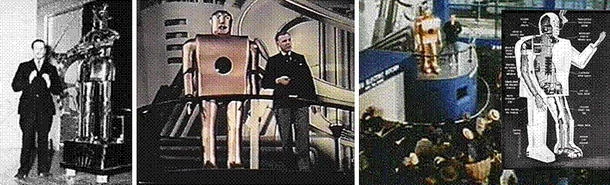
\includegraphics[width=.85\linewidth]{pictures/elektro.png}
    \caption{``Alpha'', el primer robot diseñado con fines militares y su posterior evolución, ``Elektro''.}
    \label{fig:elektro}
\end{figure}

Toda esta evolución ha desembocado en la robótica moderna, en donde tenemos robots sofisticados y con
distintos actuadores, pudiendo interactuar con muchísimos elementos de nuestro entorno y trabajar en
distintas fases de producción de cadenas de montaje en serie. Además, se trabaja continuamente para 
que cada vez los robots puedan realizar más tareas de los humanos, mejorando cada vez más los
``\textit{end--effectors}'' (controladores del final de los extremos del brazo). En la figura 
\ref{fig:new_robots} se puede ver cómo robots medianamente antiguos (del 2005) ya podían realizar diversas
actividades, como interactuar con las personas o tocar un instrumento.

\begin{figure}[H]
    \centering
    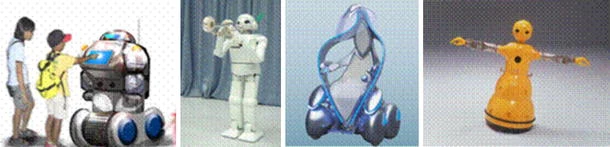
\includegraphics[width=.75\linewidth]{pictures/expo_japan.png}
    \caption{Exposición mundial del 2005 en Japón \cite{belarmino_j_and_moran_me_and_firoozi_f_and_capello_s_and_kolios_e_and_perrotti_m_oriental_2005}.}
    \label{fig:new_robots}
\end{figure}

\subsection{Los brazos robóticos}

Con los avances actuales, el mundo de la robótica ha evolucionado a un nuevo nivel: con la inclusión
de los transistores en lugar de las válvulas de vacío se han podido desarrollar circuitos integrados
que manejan de manera mucho más sofisticada el control del brazo robótico.

En 1962, la empresa ``Unimate'' introdujo su primer brazo robótico de carácter industrial. Aproximadamente,
se vendieron 8500 unidades. Este hito es importante en tanto a que se valoraron por primera vez los
grados de libertad que debían de tener los brazos robóticos. 

Estos planteamientos derivaron en distintos robots famosos que incluso siguen en activo hoy día. En
1969, Victor Scheinman, de la Universidad de Standford, desarrolló un brazo robótico que funcionaba
alimentado por la electricidad y que se podía mover en los seis ejes, el cual se llamó ``el brazo de
Standford''. De forma paralela, Marvin Minsky, del MIT, desarrolló un brazo robótico para la investigación
naval, para exploración submarina. En particular, el brazo tenía veinte grados de libertad ya que el brazo
funcionaba mediante electricidad impulsando sistemas hidráulicos. Más tarde, Scheinman continuó
desarrollando brazos robóticos, creando el ``\textit{Programmable Universal Machine for Assembly}'',
más conocido como PUMA.

En la actualidad, los brazos robóticos se desarrollan y diseñan para seguir la estructura física
del cuerpo humano (ver figura \ref{fig:human_body}).

\begin{figure}[H]
    \centering
    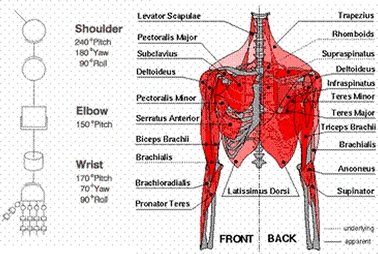
\includegraphics[width=.65\linewidth]{pictures/human_body.png}
    \caption{Grados de libertad de un brazo robótico y estructura del cuerpo humano \cite{moran_evolution_2007}.}
    \label{fig:human_body}
\end{figure}

De esta estructura anterior, se deducen las siguientes partes:

\begin{itemize}
    \item Articulación del hombro: dispone de tres grados de libertad que permiten
    subir y bajar, ir a la izquierda y derecha, y rotar sobre sí mismo.
    \item Articulación del codo: el codo permite extender, contraer y reorientar tanto
    la muñeca como la mano. Por lo general, se estima la extensión del codo en unos
    150\textdegree.
    \item La muñeca: compone el último elemento del brazo robótico antes de llegar
    al ``\textit{end--effector}''. Es de los elementos más importantes debido a su
    gran capacidad de movimiento en las tres dimensiones. Sin esta articulación,
    el brazo robótico se asemejaría en funcionalidad a un robot pantográfico. Cada vez más,
    las articulaciones de la muñeca se vuelven complejas y sofisticadas. La muñeca humana,
    por ejemplo, puede moverse 45\textdegree desde el centro, pero se reduce mucho la
    capacidad de rotación de la misma. En la actualidad se está investigando cómo poder
    mejorar la relación de movimientos para permitir una mayor movilidad, pero las 
    singularidades siguen siendo un gran problema. Por ejemplo, el robot quirúrgico
    da Vinci, pese a lo avanzado que pueda parecer, tiene problemas de bloqueo de las muñecas
    del mismo cuando se acerca a posiciones singulares.
    \item La mano: supone un ``\textit{end--effector}'' diferenciado que define el propóstio
    y la capacidad del brazo robótico. La mano es una herramienta capaz de realizar múltiples
    acciones muy variadas entre sí. Actualmente, se sigue investigando de forma activa sobre
    ello para intentar implementar controles sensoriales, de presión y de movimiento en los
    ``\textit{end--effector}'' de los robots.
\end{itemize}

\subsection{La actualidad}

Durante los dos últimos decenios la robótica ha evolucionado de manera exponencial. Se ha
trabajado de forma activa en mejorar ciertas condiciones industriales, espaciales y
en el día a día de las personas. Por un lado, en el 2001 se puso en la ISS el brazo
robótico ``Canadarm2'', conocido oficialmente como 
``\textit{Space Station Remote Manipulator System}'' (SSRMS) (figura \ref{fig:canadarm2}).

\begin{figure}[H]
    \centering
    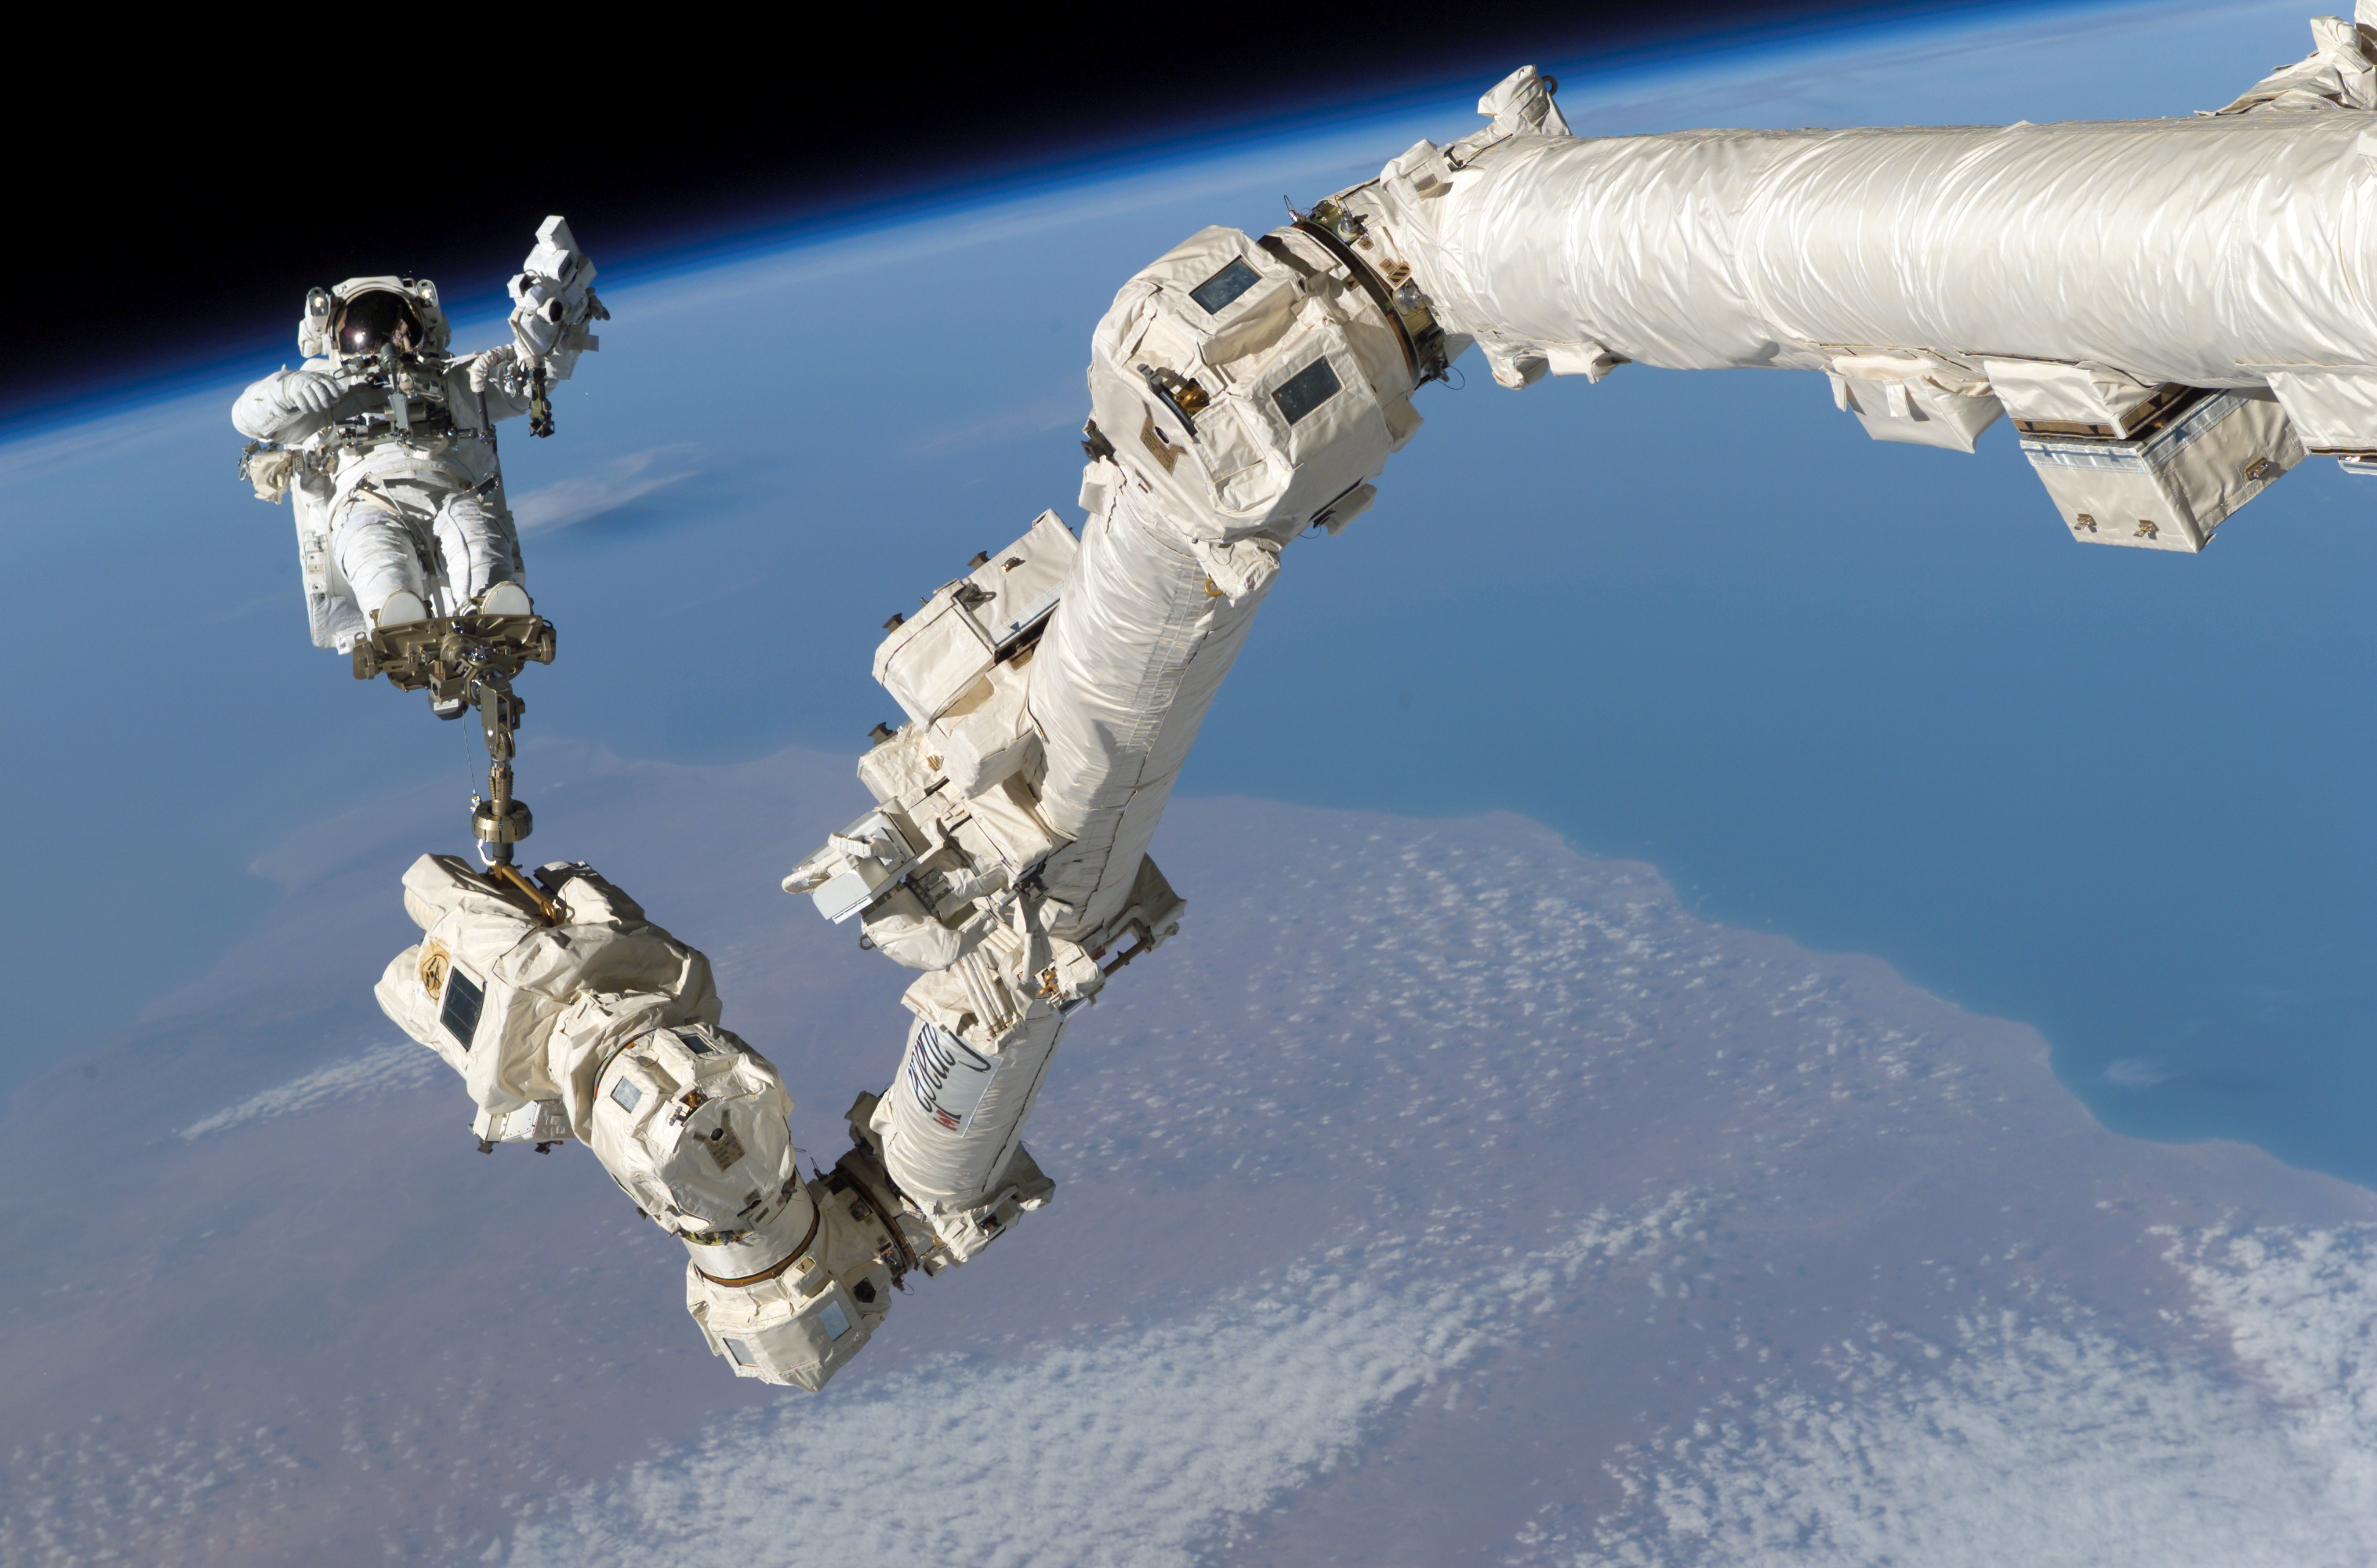
\includegraphics[width=.63\linewidth]{pictures/STS-114_Steve_Robinson_on_Canadarm2.jpg}
    \caption{Vista exterior del Canadarm2 \cite{noauthor_mobile_2020}.}
    \label{fig:canadarm2}
\end{figure}

Además, en 2005, se desplegaron en Marte los rovers ``Spirit'' (figura \ref{fig:spirit}) y 
``Opportunity'' (figura \ref{fig:opportunity}). 

\begin{figure}
    \centering
    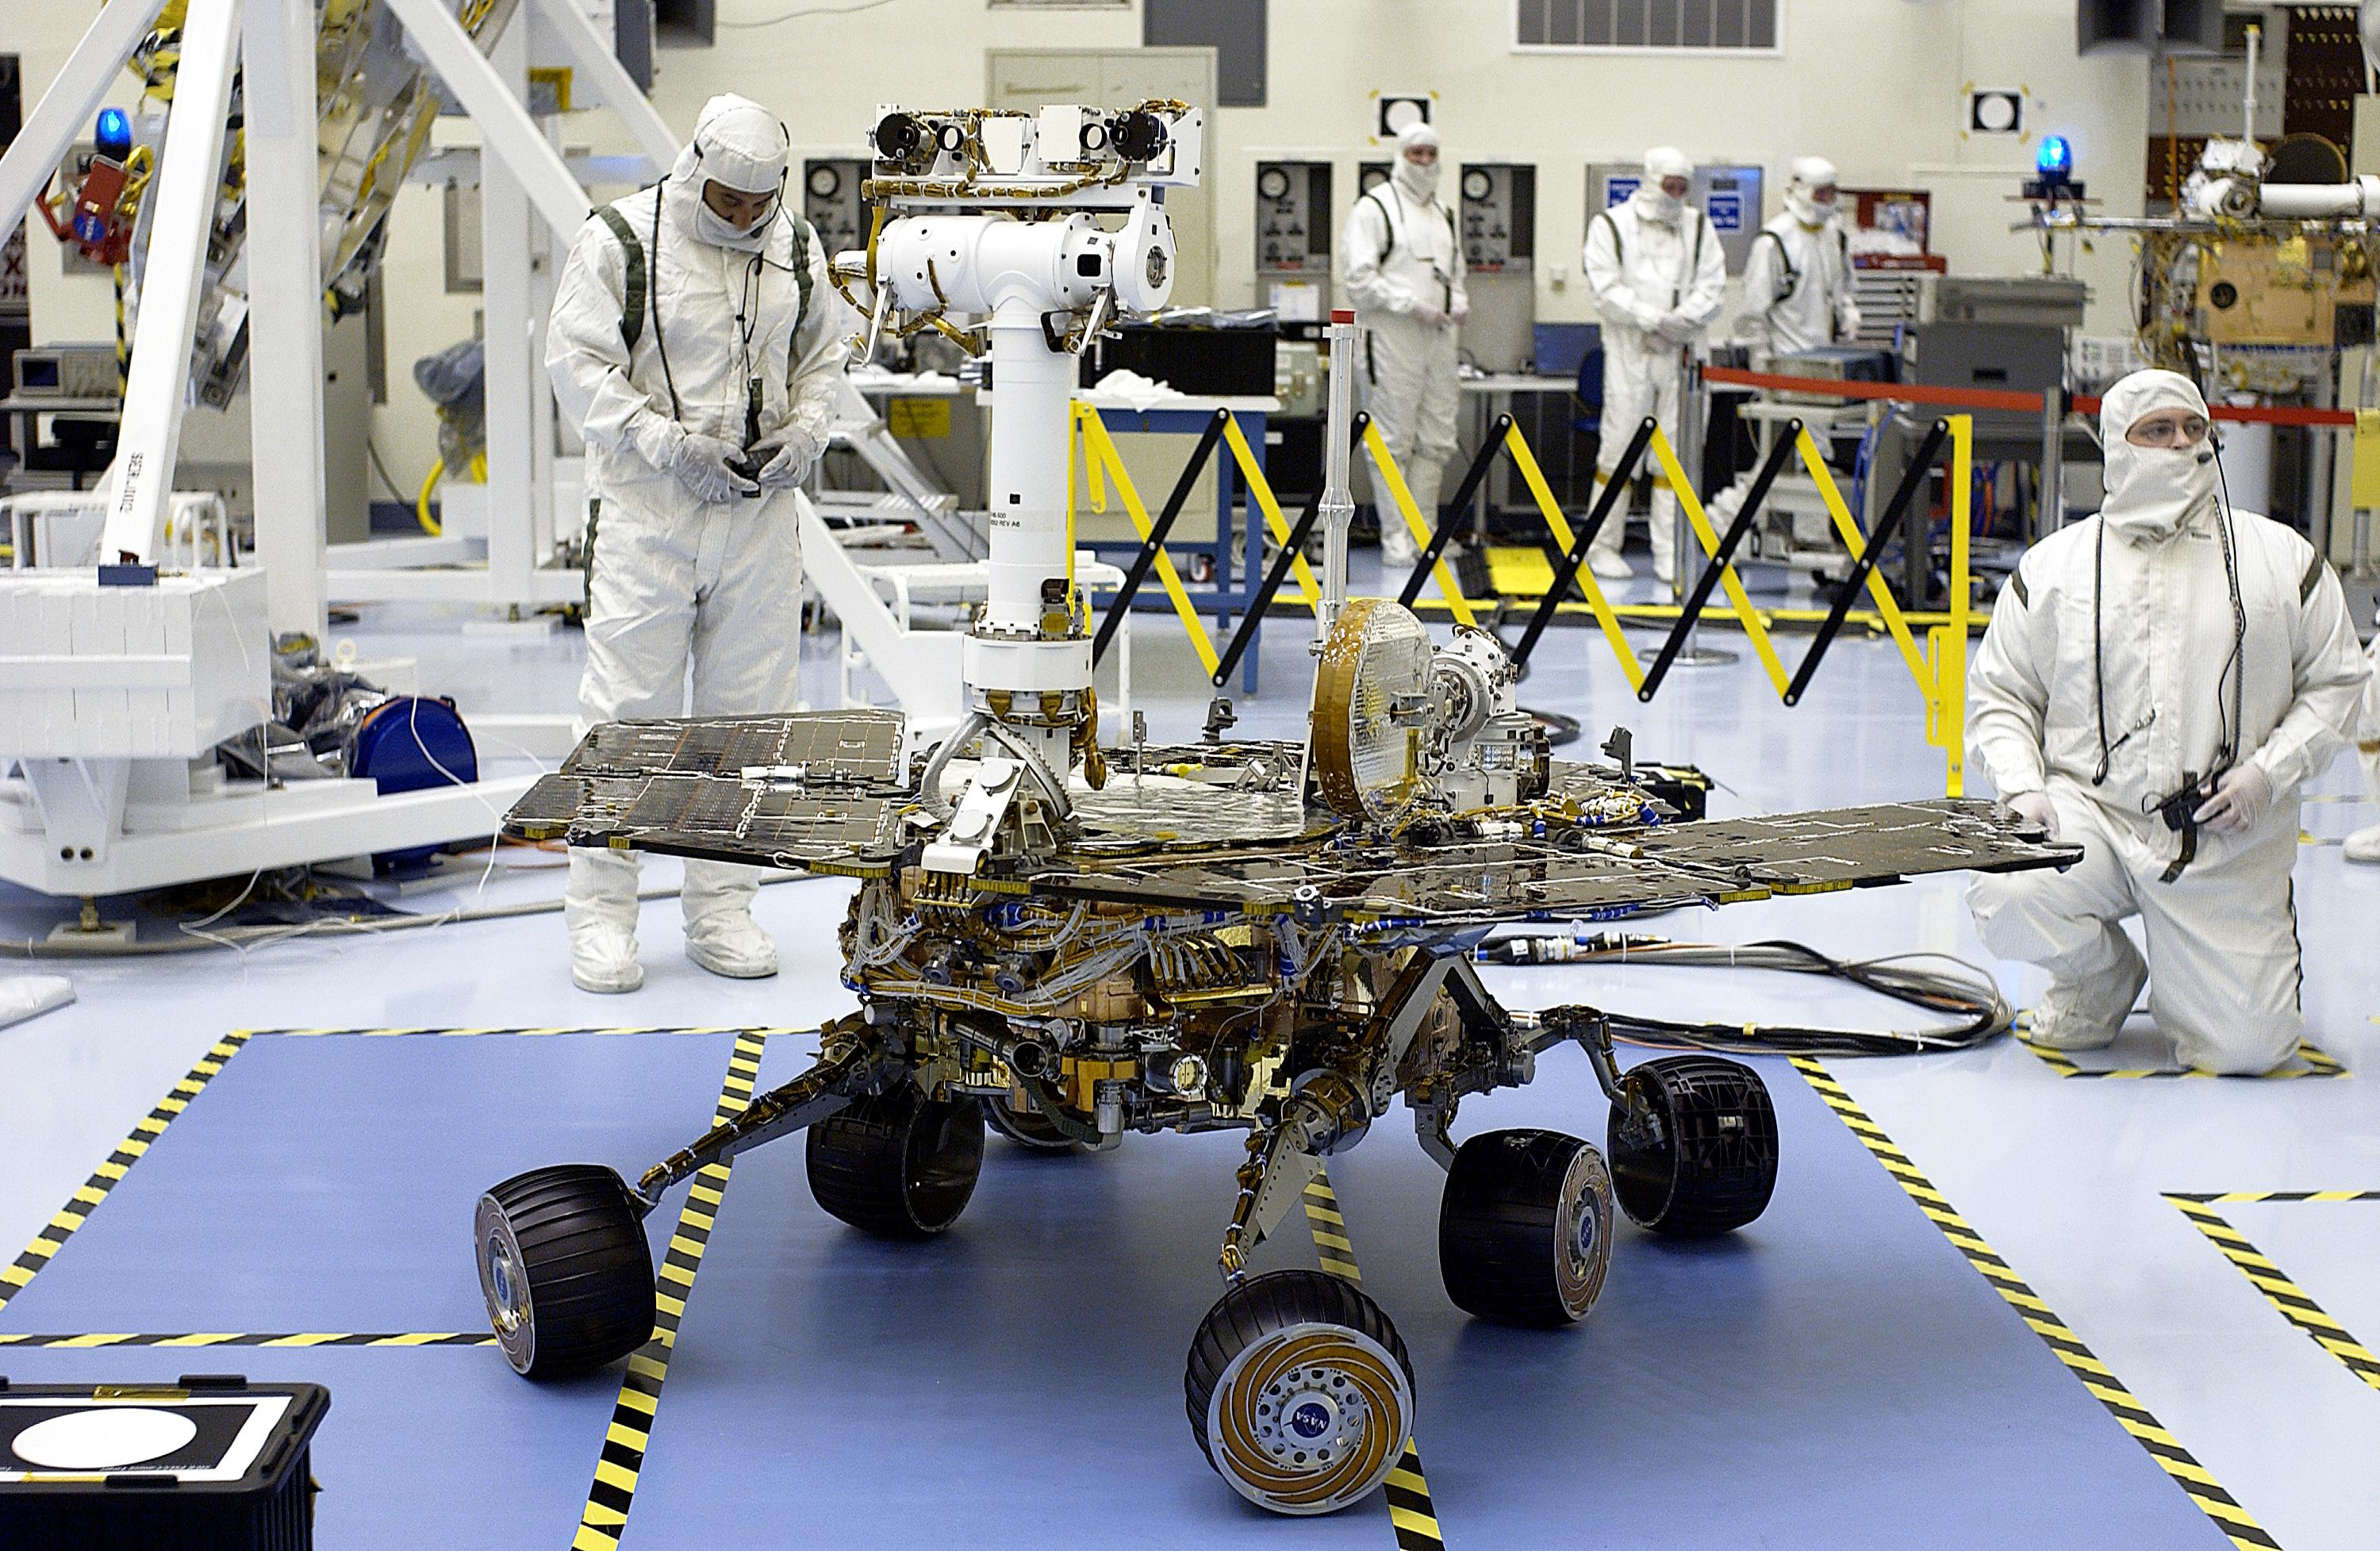
\includegraphics[width=.75\linewidth]{pictures/spirit_rover.jpg}
    \caption{Rover ``Spirit'', desarrollado por la NASA y desplegado en 2004 \cite{noauthor_spirit_2020}.}
    \label{fig:spirit}
\end{figure}

El primero supuso un gran avance de la
ingeniería, ya que crearon un robot completamente autónomo para enviarlo a un terreno
muy hostil. Con las seis ruedas que tenía permitía una movilidad bastante elevada en
terrenos muy desiguales, usando las ruedas delanteras y traseras como ejes directrices 
y las centrales como ejes motrices (detalle en la figura \ref{fig:spirit}). Además,
la fisionomía de las mismas y su elevación permitía que el dispositivo se desplazara por
distintos tipos de terreno de una manera óptima, pudiendo elevar y bajar ejes a placer
para una mejor sujeción y tracción.

\begin{figure}[H]
    \centering
    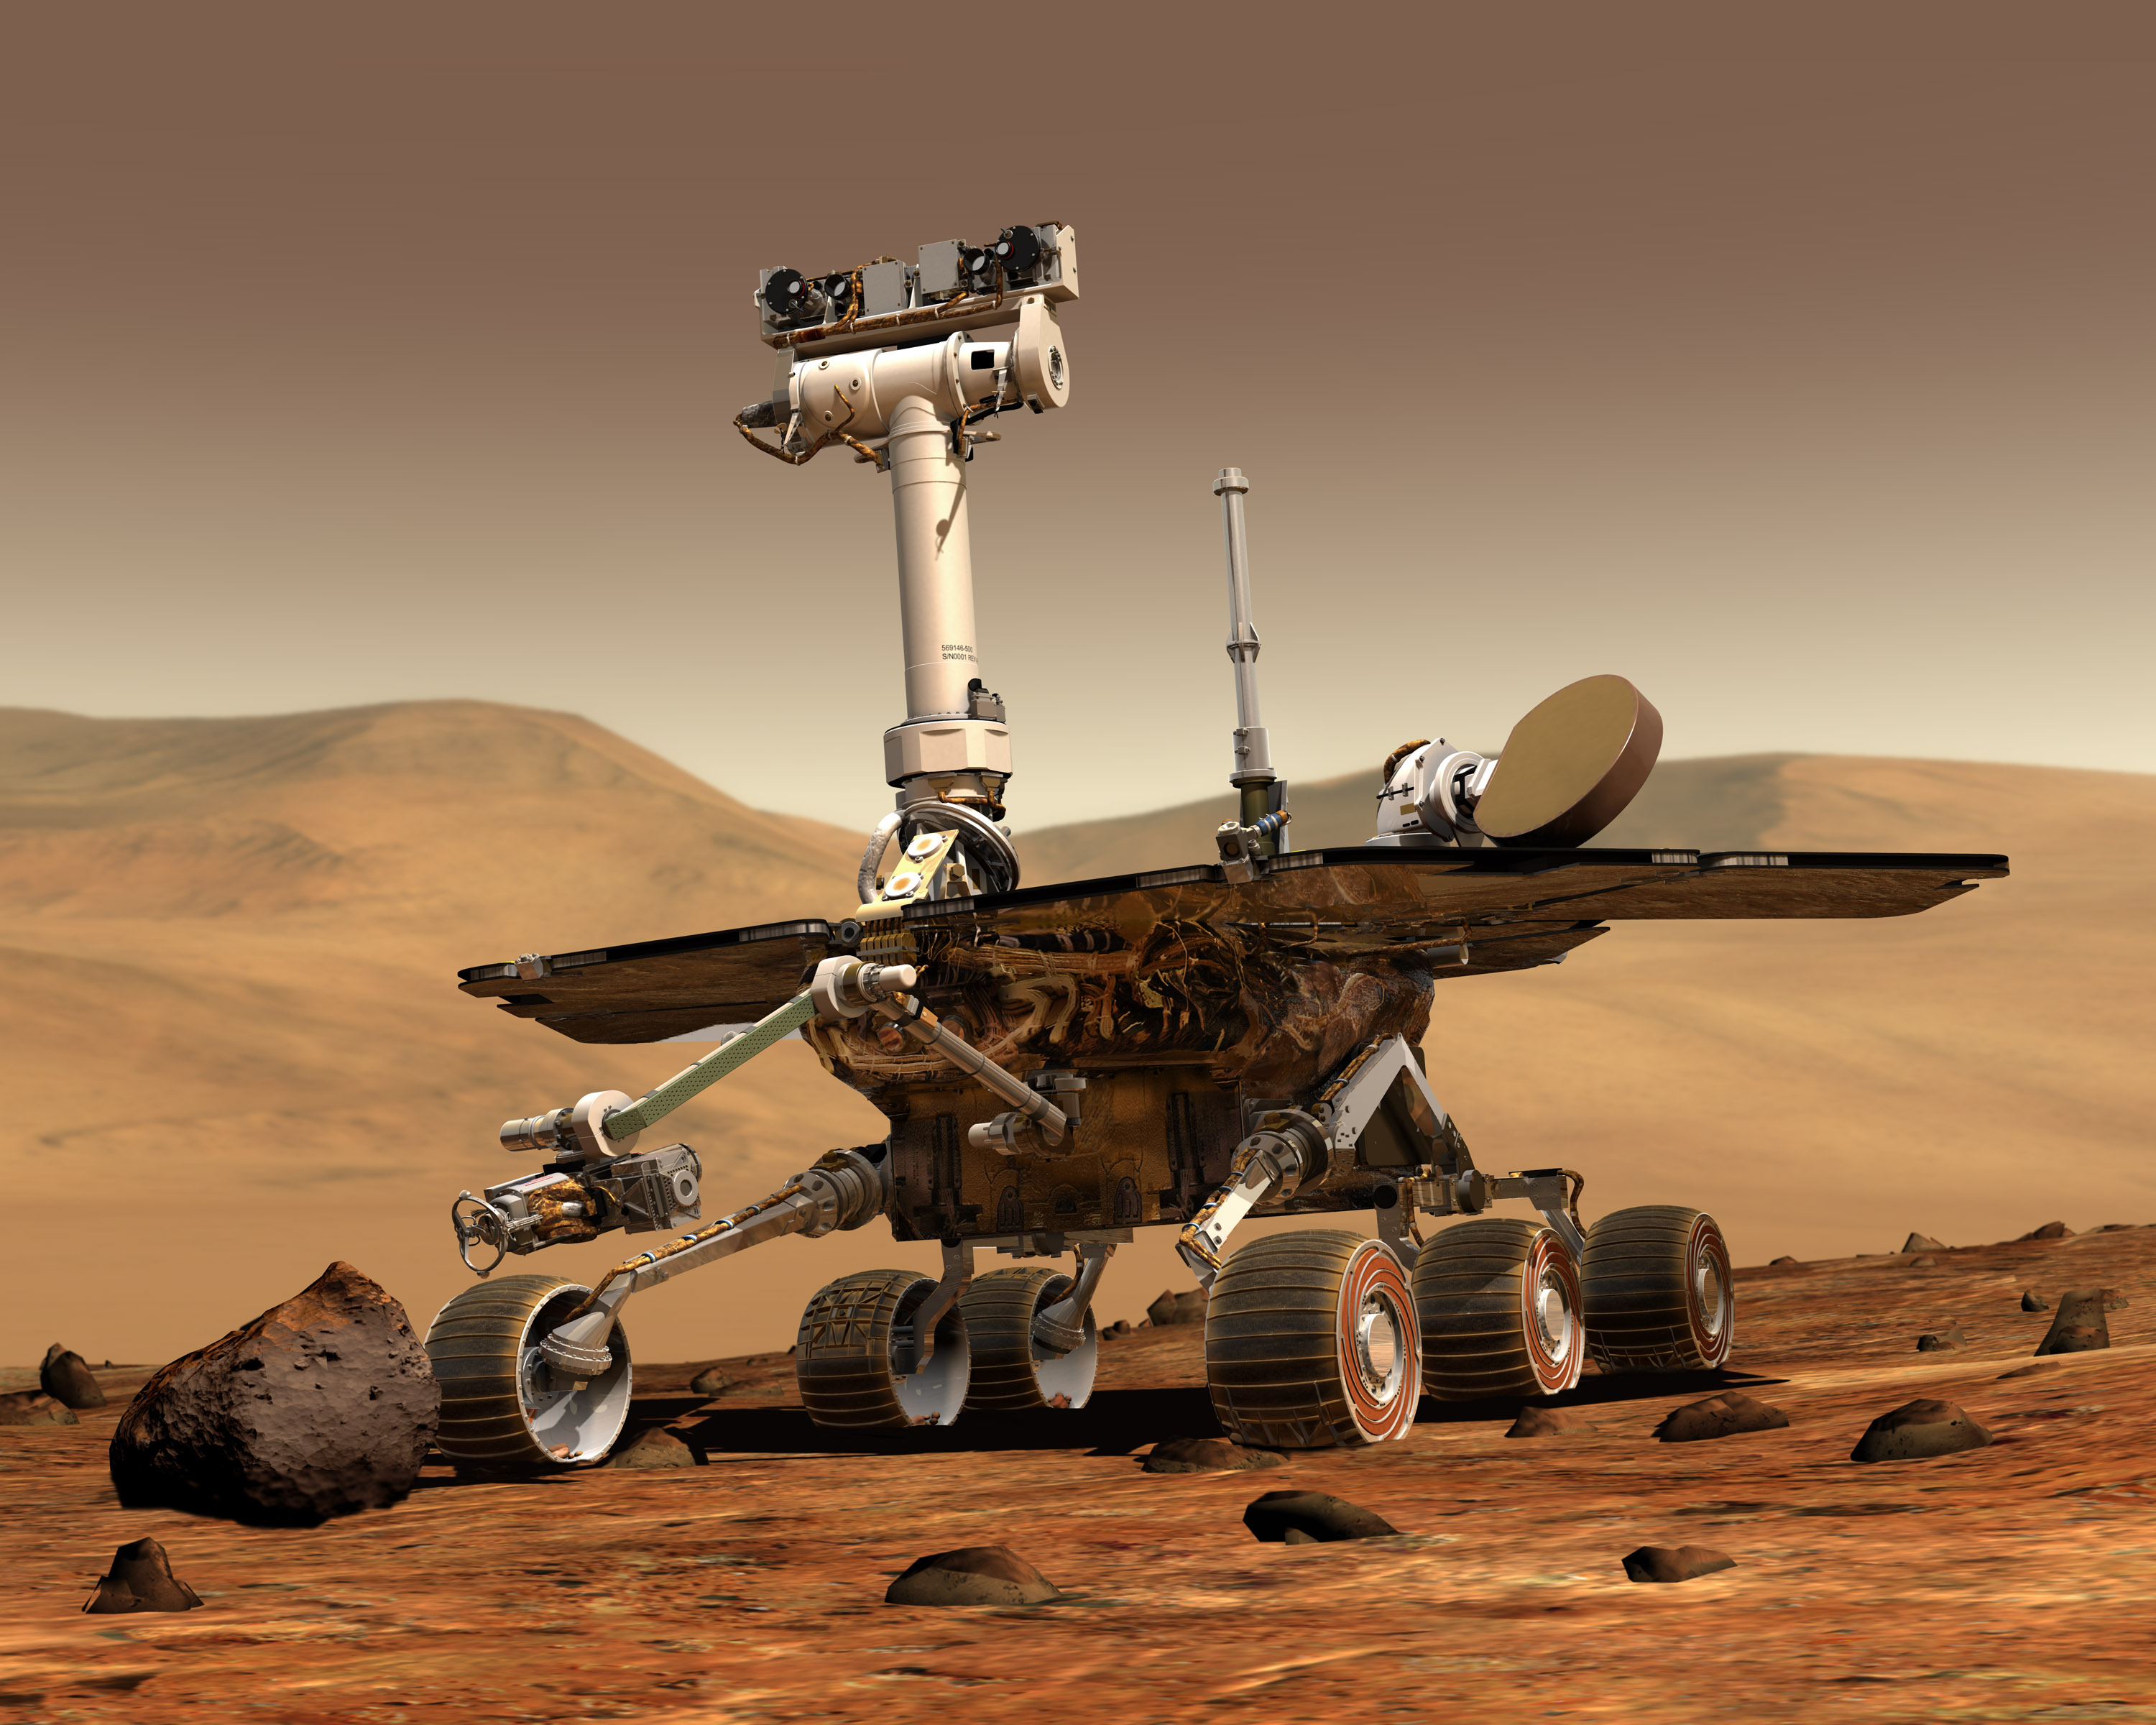
\includegraphics[width=.5\linewidth]{pictures/opportunity.jpg}
    \caption{Rover ``Opportunity'', desarrollado por la NASA y desplegado en 2004 \cite{noauthor_opportunity_2020}.}
    \label{fig:opportunity}
\end{figure}

Por otra parte, se puede apreciar cómo el ``Opportunity'' tenía una estructura bastante
similar al ``Spirit'' pero añadía alguna que otra mejora. La diferencia principal entre ambos 
era el lugar de aterrizaje (figura \ref{fig:landing_sites}), ya que ambos servían para 
recorrer distintos puntos de la superficie marciana para recopilar datos y tomar muestras.

\begin{figure}[H]
    \centering
    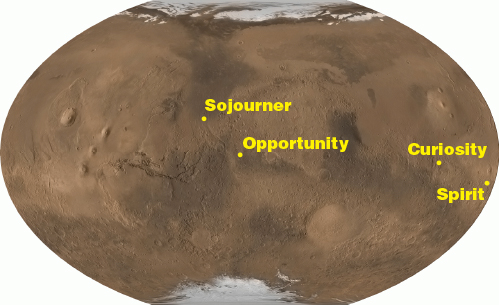
\includegraphics[width=.75\linewidth]{pictures/rover-landing-sites.en.jpg}
    \caption{Lugares de aterrizaje de los rovers de la misión espacial a Marte \cite{noauthor_mars_nodate}.}
    \label{fig:landing_sites}
\end{figure}

La misión del ``Spirit'' duró 2623 soles frente a los 90 inicialmente planeados \cite{noauthor_spirit_2020},
y la misión del ``Opportunity'' duró 5352 soles frente a los también 90 inicialmente planteados \cite{noauthor_opportunity_2020}.
Esto se traduce en 2695 días terrestres (6 años, 9 meses y 12 días) y 5498 días terrestres (15 años)
respectivamente.

Por otra parte, los robots de aplicación doméstica también han ido creciendo cada vez más,
naciendo en 2002 el popular Roomba (figura \ref{fig:roomba}), de la empresa iRobot, o distintos brazos articulados
para, por ejemplo, ayudar a personas que carezcan de dichos miembros o asistir a personas
mayores en sus hogares.

\begin{figure}[H]
    \centering
    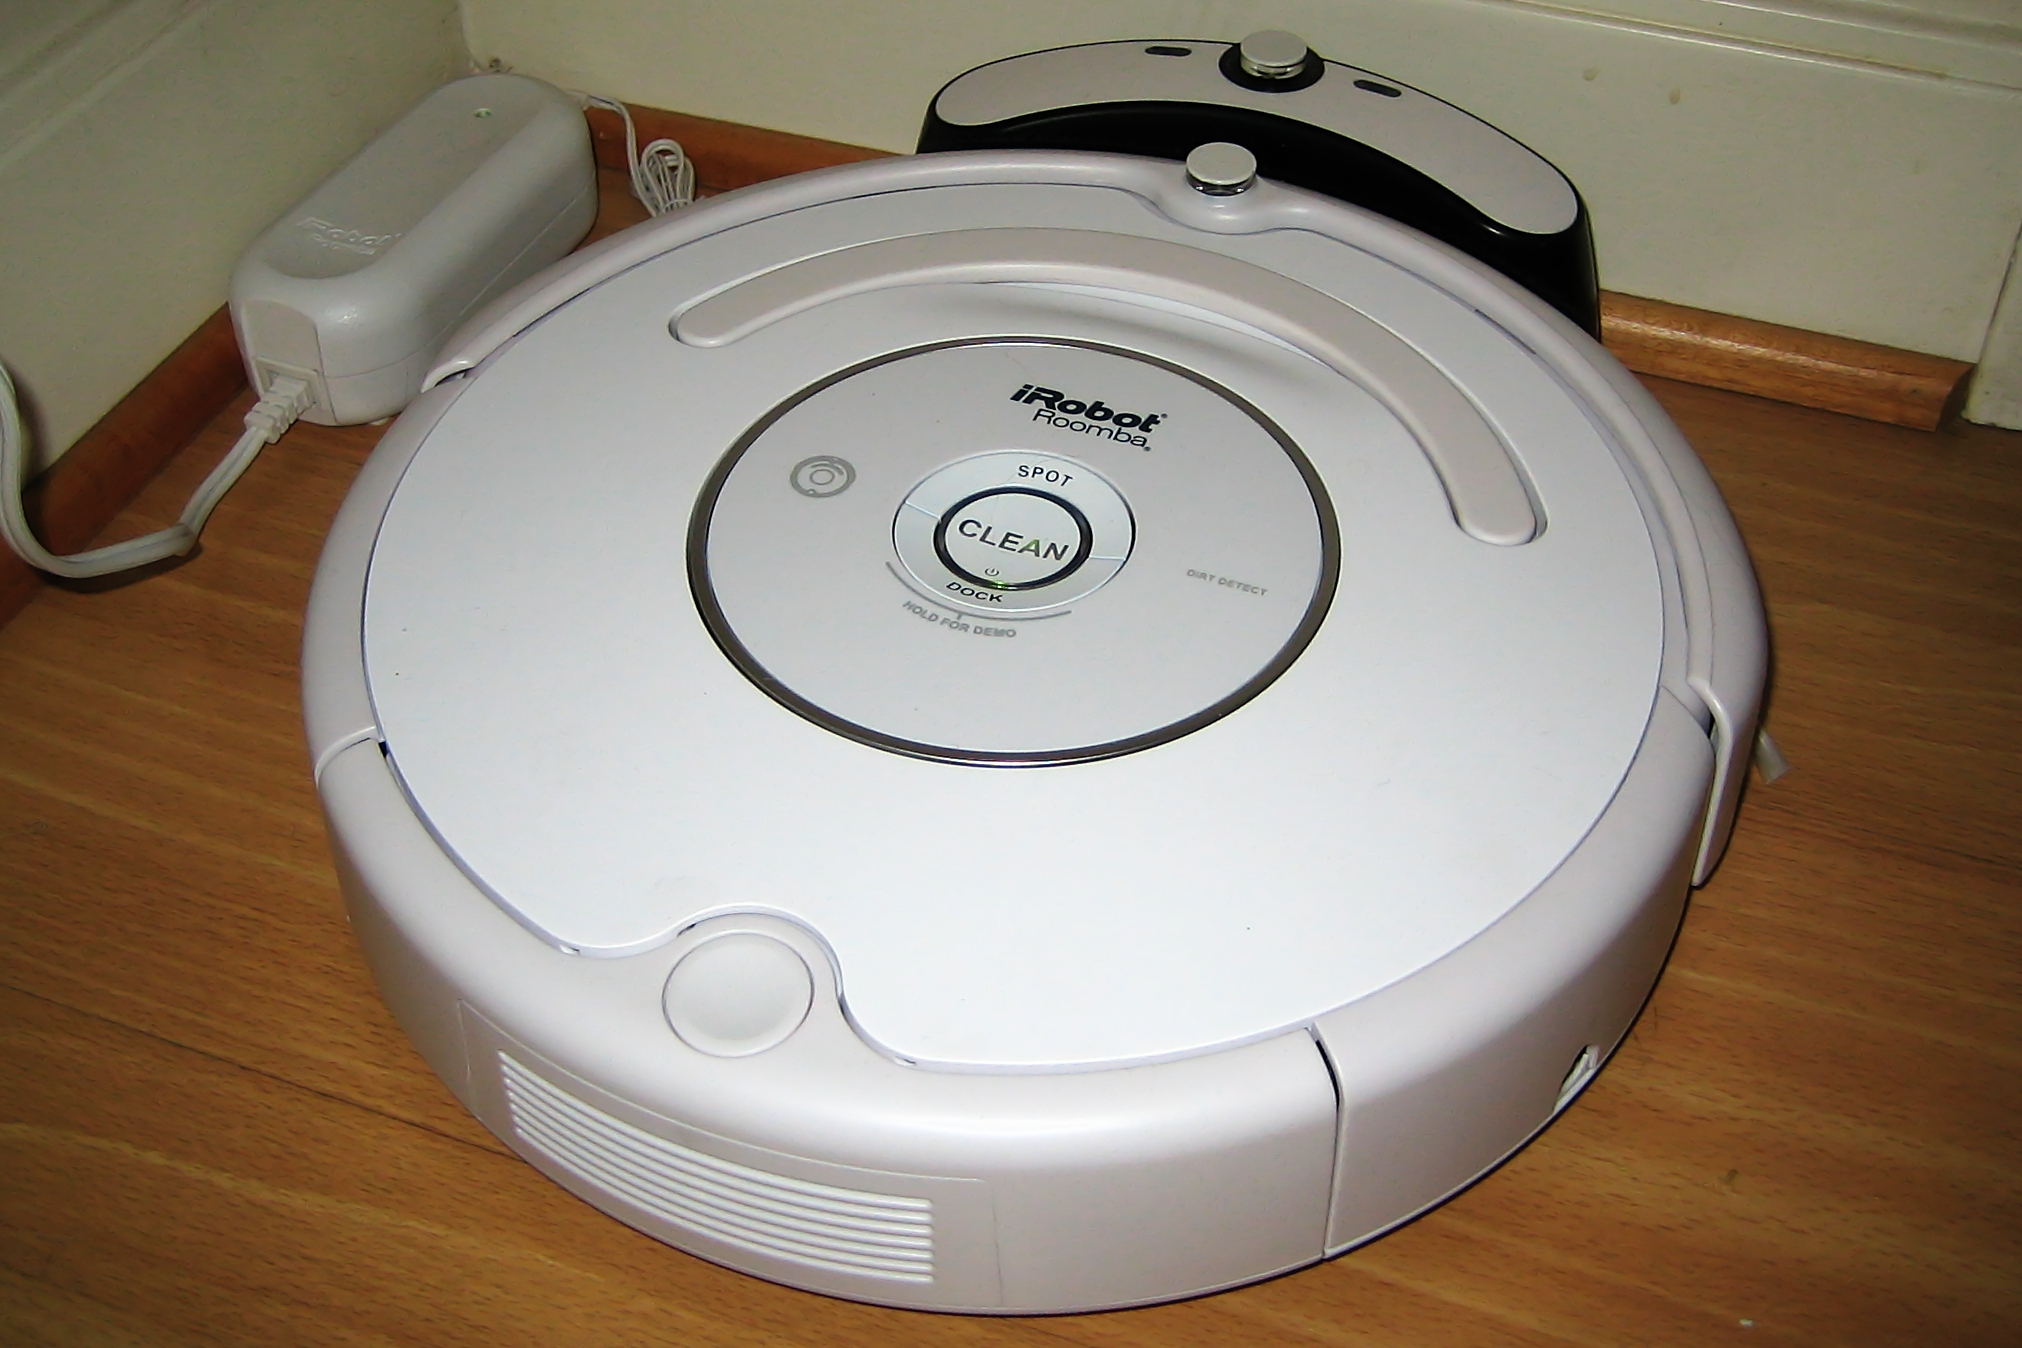
\includegraphics[width=.5\linewidth]{pictures/Roomba3g.jpg}
    \caption{Robot Roomba en la estación de carga \cite{noauthor_history_2020}.}
    \label{fig:roomba}
\end{figure}

Además, la industria de los coches autónomos también ha crecido de forma exponencial,
sobre todo con la llegada al mercado en 2003 de Tesla Motors y sus coches eléctricos
que disponen del sistema ``Autopilot'' (figura \ref{fig:ap}), encontrándose actualmente en el nivel 2 de
autonomía según la lista del SAE \cite{noauthor_teslas_nodate}\cite{noauthor_self-driving_2020}.

\begin{figure}[H]
    \centering
    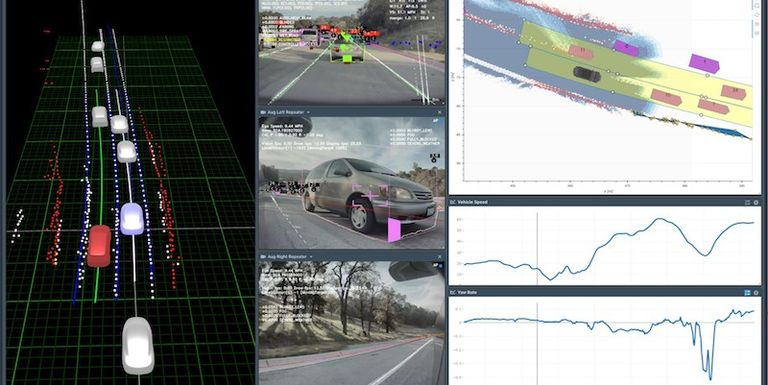
\includegraphics[width=\linewidth]{pictures/tesla-automation.jpeg}
    \caption{Lo que ve un Tesla cuando está en conducción autónoma nivel 2 \cite{baldwin_teslas_2020}.}
    \label{fig:ap}
\end{figure}

Por otro lado, se ha avanzado mucho a nivel de robots militares y humanoides. Un ejemplo
de ello es la empresa \textit{Boston Dynamics}, la cual ha desarrollado múltiples robots
con un grado de libertad bastante elevado. Dichos robots se caracterizan por una gran 
estabilidad y la amplia variedad de movimientos que pueden realizar: andar, correr,
saltar, subir escaleras, abrir puertas, etc. Actualmente, dos robots son los principales:
``\textit{Big-Dog}'' (figura \ref{fig:big-dog}) y ``Atlas'' (figura \ref{fig:atlas}).

\begin{figure}[H]
    \centering
    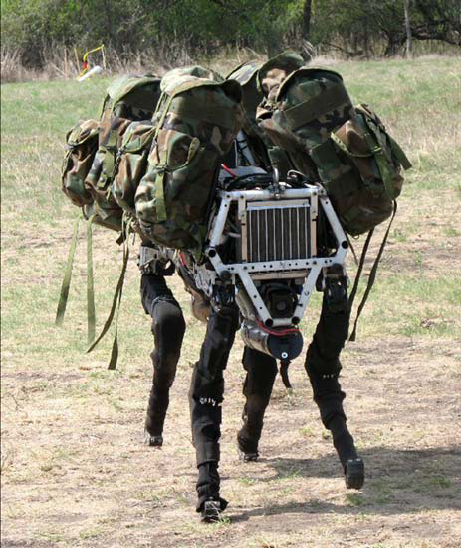
\includegraphics[width=.3\linewidth]{pictures/big-dog.png}
    \caption{Robot ``\textit{Big-Dog}'' de Boston Dynamics \cite{noauthor_boston_2020}.}
    \label{fig:big-dog}
\end{figure}

El primero tiene un amplio uso militar: debido a su forma, es muy útil para llevar cargas
pesadas durante largas distancias. Además, la configuración cuadrúpeda y los avanzados 
sistemas \textit{software} y \textit{hardware} del que dispone permite que el robot sea
estable incluso en condiciones bastante complicadas, como puede ser un suelo helado.

\begin{figure}[H]
    \centering
    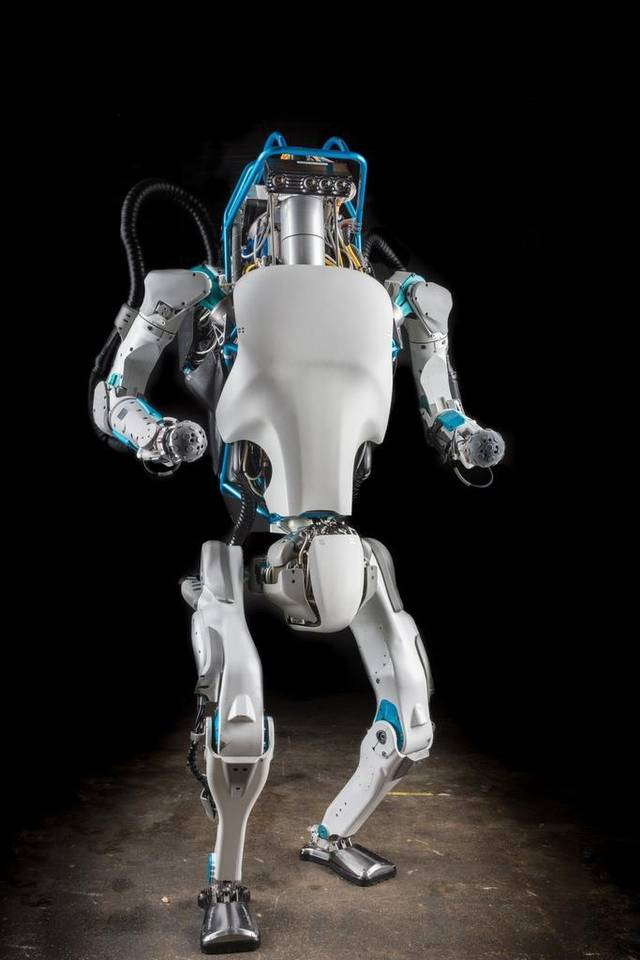
\includegraphics[width=.3\linewidth]{pictures/atlas.jpg}
    \caption{Robot ``Atlas'' de Boston Dynamics \cite{noauthor_boston_2020}.}
    \label{fig:atlas}
\end{figure}

``Atlas'', por otra parte, es un trabajo en progreso que permitirá, en un futuro, poder
utilizarlo con fines militares y domésticos. Puede llevar objetos pesados con sus brazos
y moverse con mucha agilidad, haciéndolo un robot muy polivalente según se quiera utilizar.

Finalmente, el desarrollo de los brazos articulados con múltiples finalidades
también ha evolucionado mucho. Desde robots industriales tales como los desarrollados
por la empresa KUKA, como el ``KR-1000 Titan'' (figura \ref{fig:kuka}),
o el brazo ``M-2000'', de FANUC hasta brazos más pequeños pero igualmente hábiles, como
el $\mu$Arm, de UFACTORY (figura \ref{fig:uarm}).

\begin{figure}[H]
    \centering
    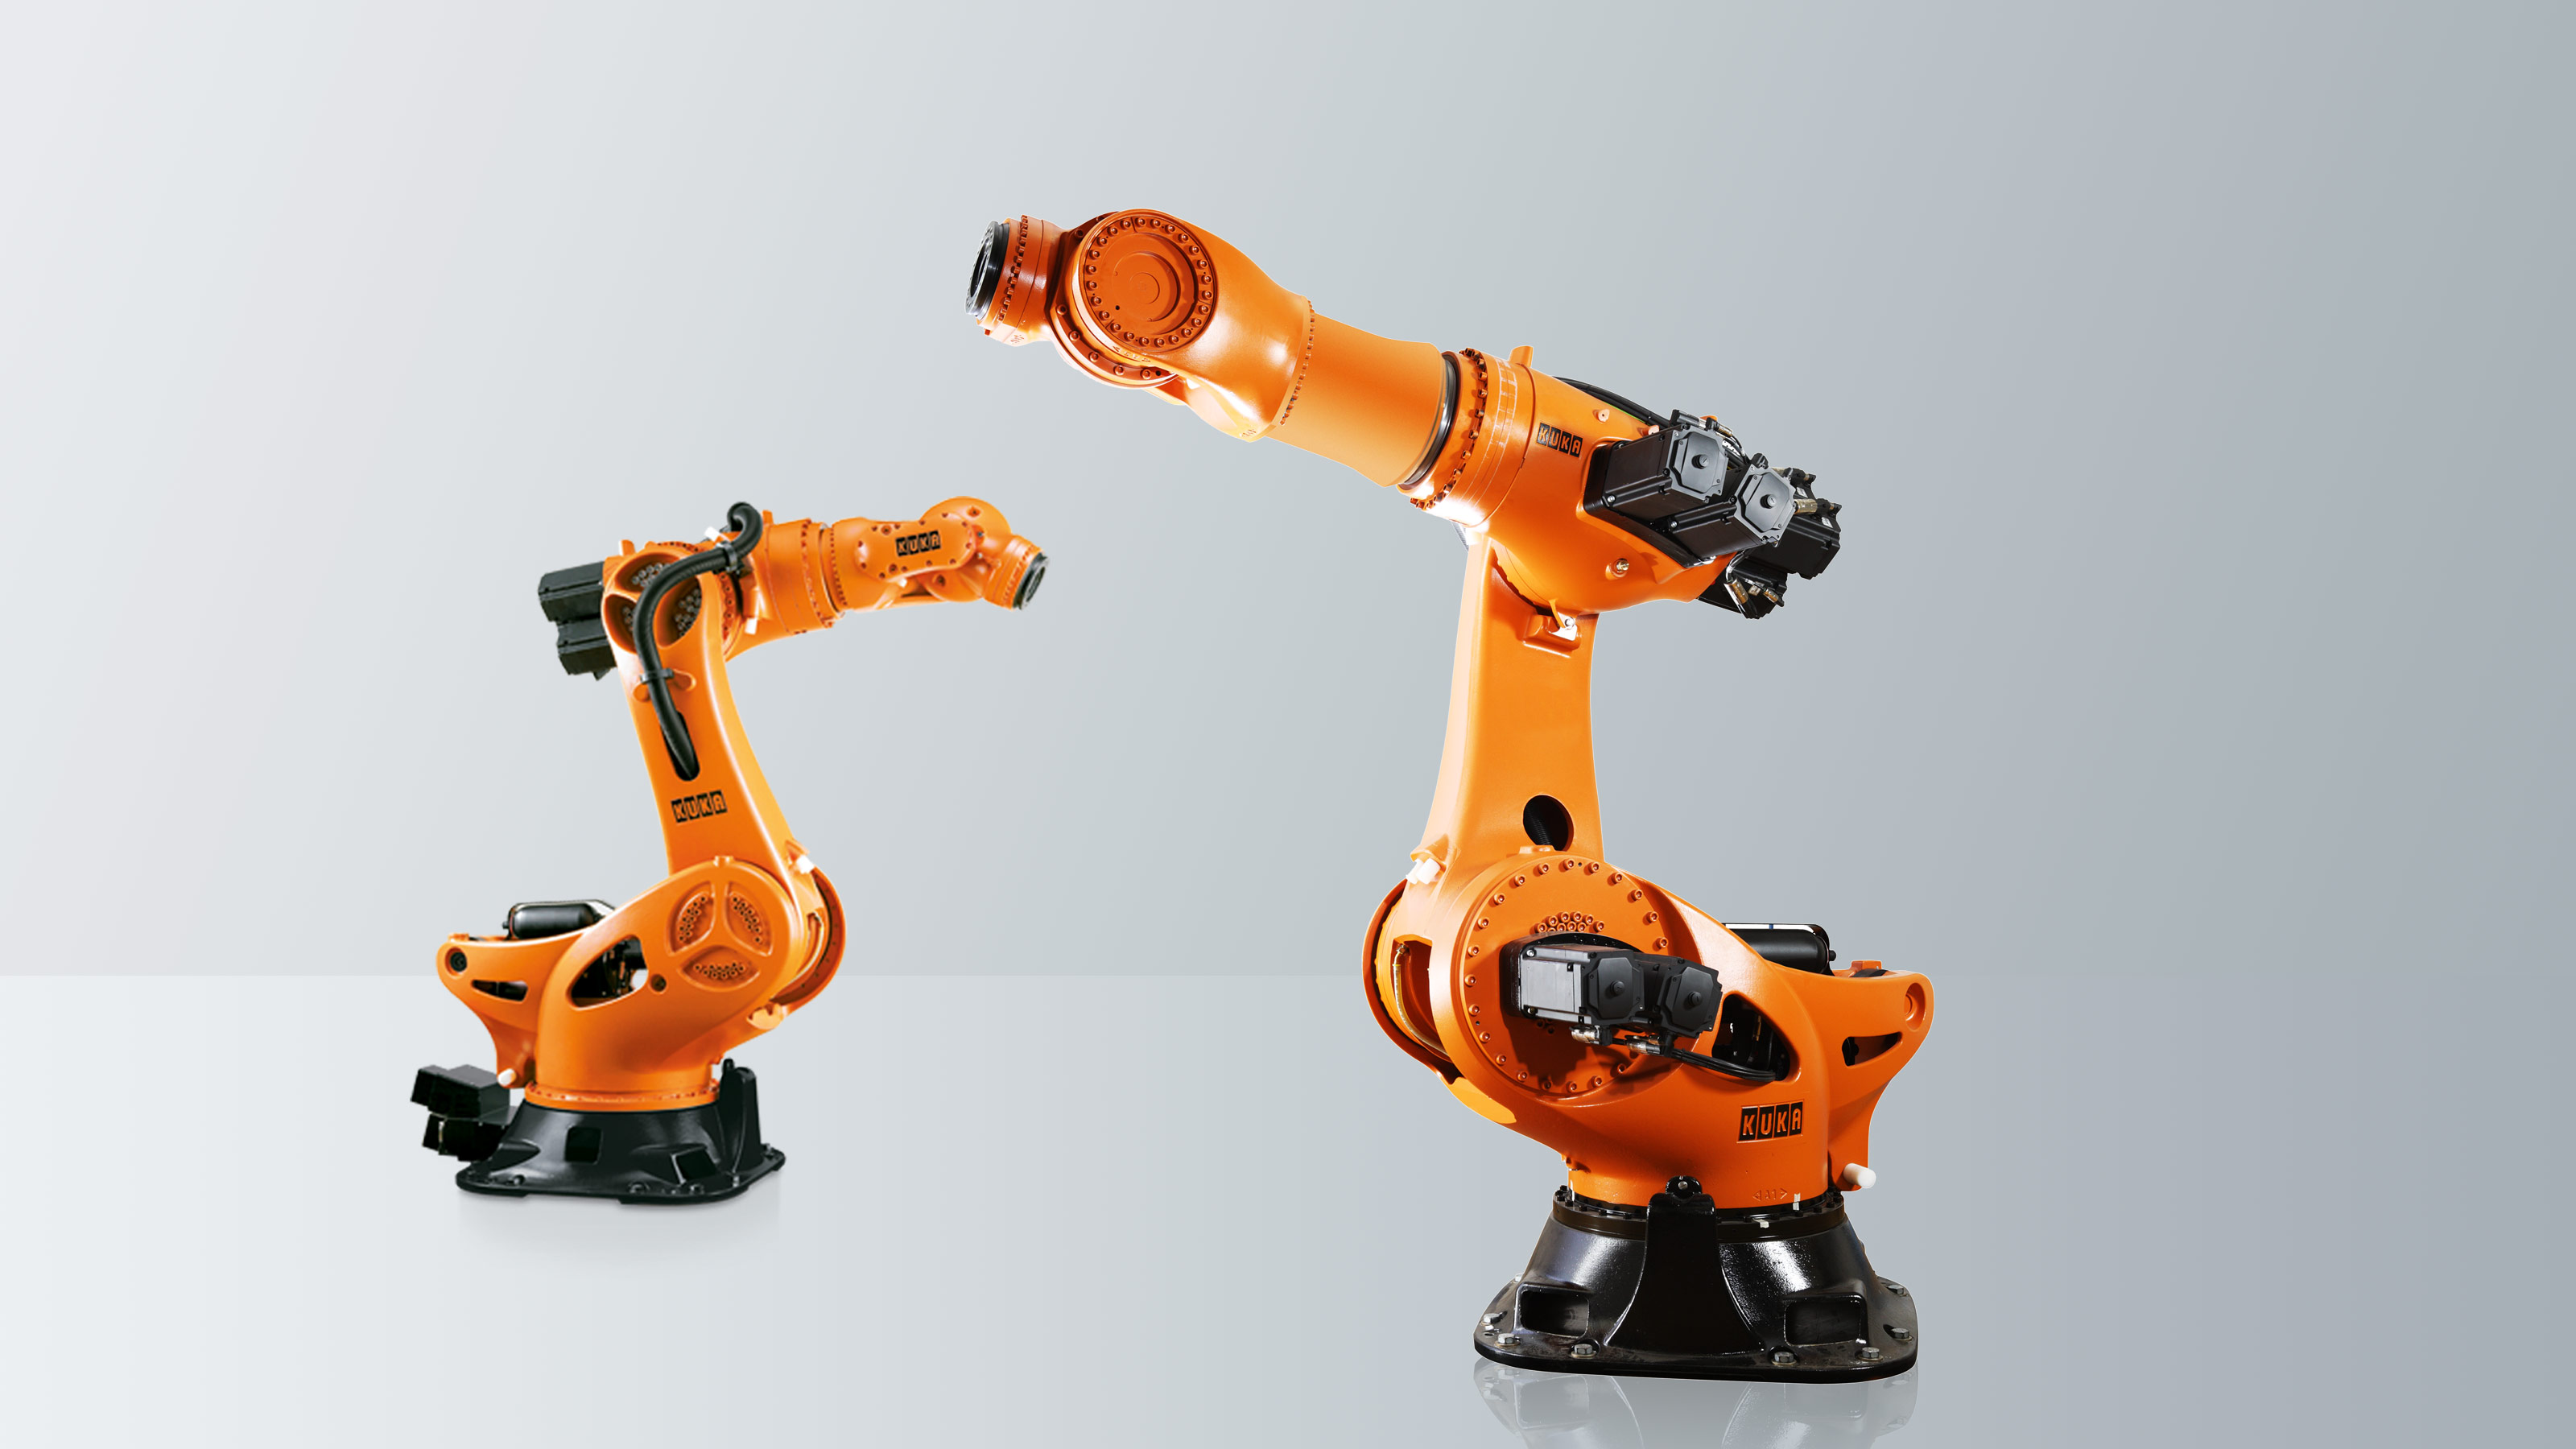
\includegraphics[width=.75\linewidth]{pictures/kr1000.jpg}
    \caption{Robot ``KR-1000 Titan'' de KUKA \cite{noauthor_kr_nodate}.}
    \label{fig:kuka}
\end{figure}

\begin{figure}[H]
    \centering
    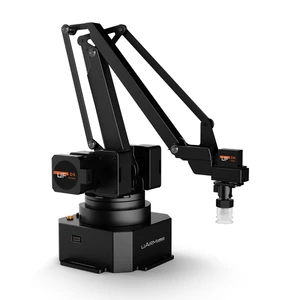
\includegraphics[width=.5\linewidth]{pictures/uarm.png}
    \caption{Robot $\mu$Arm de UFACTORY \cite{noauthor_ufactory_nodate-1}.}
    \label{fig:uarm}
\end{figure}

Estos robots tienen múltiples propósitos: el primero, levantar y trasladar piezas
muy grandes y pesadas con muchísima precisión. El segundo, disponer de un robot
para poder aprender y utilizarlo para tareas como, por ejemplo, impresión 3D. 
Se desarrolló con la intención de ser accesible e intentar introducir en el mundo
de la robótica a aquellos que pudieran estar interesados, pero su alto coste impide
el acceso a aquellos con capacidad adquisitiva más baja.
%% REVISADO - J
\section{Motivaciones y objetivos del desarrollo del proyecto}
Durante el primer semestre del cuarto curso de Ingeniería de Computadores,
hay dos asignaturas las cuales propiciaron el desarrollo de este proyecto: robótica
y sistemas empotrados.

Con la primera, se vio la potencia de los brazos robóticos y se desarrolló un estudio
sobre un controlador el cual se ha hablado con anterioridad: el $\mu$Arm \cite{UPMRoboticsUarm2019b}.
Con la segunda asignatura, se vio cómo con sistemas de aplicación específica se podían
desarrollar circuitos con suficiente potencia como para poder tomar el control de otros
dispositivos más grandes y complejos aplicando la lógica estudiada a lo largo de los
años.

Se tomaron en cuenta los conocimientos obtenidos de las asignaturas anteriores
para empezar un desarrollo que uniera esos dos campos: diseñar un brazo robótico
impreso en 3D el cual estuviera gobernado por un microcontrolador en una placa de
control de propósito específico. Para ello, se parte de los diseños 3D provistos
en la web de UFACTORY \cite{UFACTORYXArmTextbackslashtextbaruArm} para su posterior
adaptación y reutilización. En lo referente a la placa de control, el brazo original
utiliza una placa Arduino Mega \cite{ArduinoMega2560}, por lo que se decidió (para dar
mayor peso a la parte de ingeniería e intentar reducir costes) diseñar e implementar al completo una placa con
otro microcontrolador para gobernar dicho brazo robótico.

Principalmente, este trabajo se desarrolla bajo las dos perspectivas siguientes:
\begin{itemize}
    \item Aplicar en un proyecto de ingeniería real las competencias y técnicas que 
    se han ido aprendiendo a lo largo de los distintos cursos del Grado de Ingeniería
    de Computadores (61CI).
    \item Construir una alternativa asequible y accesible, tanto a niveles de \ac{OS} y
    \ac{OH}, de un brazo robótico de manera que cualquier persona interesada en este
    ámbito de la ingeniería pueda introducirse y aprender, e incluso montar el brazo
    por sí mismo.
\end{itemize}

Para la primera perspectiva, la forma de afrontarla y desarrollarla está detallada en el
punto siguiente (\ref{sec:methodology}). Para la perspectiva de desarrollo de un
producto accesible y asequible, se partió desde el abaratamiento de costes: el brazo
original $\mu$Arm se encuentra disponible en venta por aproximadamente \$749. Dicho precio,
pese a no ser especialmente elevado, impide a muchas personas el acceso a la robótica
en un brazo que pretende ser educativo y útil. Por este motivo, se desarrolla este proyecto
principalmente para resultar barato. Además, siguiendo con la política del brazo
original, el proyecto se desarrolla bajo las premisas \ac{OS} y \ac{OH}, de manera que
inclusive para aquellos que no puedan imprimir el brazo 3D se dispone de forma universal
todos los diagramas, planos, esquemas, diseños y código fuente que se ha empleado para
acabar desarrollando el brazo \pArm{}.
%% REVISADO - J
\section{Metodología}
\label{sec:methodology}
Dado que se pretende hacer un desarrollo de ingeniería completo, la metodología es un
punto muy importante en este proyecto.

Primeramente, antes de hacer ningún tipo de desarrollo o implementación, se hizo un
estudio del problema, y de lo que se pretendía obtener. Por una parte, se comprobó
hasta qué punto podrían ser reutilizables los diseños provistos por UFACTORY
en su página de GitHub. Esto permitió diseñar elementos nuevos, adaptar los recursos
a lo que hay disponible, etc. 
Por otro lado, se estudió qué placa de control se quería utilizar. Debido a la familiaridad
de los integrantes del equipo con las placas de la familia ``Microchip'', se plantearon
distintas alternativas:

\begin{itemize}
    \item Controladores de gama media de la familia PIC16F.
    \item Controladores de gama superior de la familia PIC32F.
    \item Controladores digitales de la señal, de la familia dsPIC.
\end{itemize}

Se optó por utilizar los últimos mencionados, ya que disponen de un control específico
matricial y matemático para poder agilizar las operaciones realizadas, de forma que
los cómputos necesarios se podrían realizar íntegramente en el microcontrolador.

Además, se estudió cómo se quería plantear la comunicación con el brazo: de forma
completamente autónoma o mediante un equipo auxiliar. Para evitar la complejidad extra
que habría surgido de desarrollar un sistema de control completamente autónomo del brazo
por sí solo, se decidió conectarlo a un equipo auxiliar externo que lo gobierne, y que
el \pArm{} no funcionase si no es estando conectado.

Una vez se definieron estos puntos, se pasó al diseño lógico del sistema que deberán
tener tanto \ac{S1} como \ac{S2}, mediante especificación de requisitos, diagramas lógicos,
diagramas físicos, diagramas de diseño, etc. Esta parte del proyecto es de las más 
importantes, ya que sustenta las ideas y las funcionalidades que habrán de estar presentes
en el producto final. Mientras tanto, se han ido desarrollando pruebas y mecanismos de
control para ir asegurando la correcta calidad del trabajo.

Finalmente, una vez completada esta parte de diseño, se pasa a la implementación real.
Dada la situación del COVID--19, esta fase de implementación se ha retrasado sobremanera,
impidiendo pues presentar el proyecto en el mes de julio, como estaba previsto, y teniendo
que acotar los plazos de implementación a, posiblemente, un mes. En el momento de
implementación, se creará la placa diseñada y se empezará la impresión de distintas piezas
3D, para comprobar su funcionamiento en conjunto e ir solucionando los posibles errores
que aparezcan.

Durante este proceso, se ha ido desarrollando además de forma paralela la memoria que 
acompaña el proyecto, permitiendo ir actualizándola con los últimos cambios y mejoras que
se han considerado de interés para aparecer descritas.

%% REVISADO
\chapter{Explicación de la estructura del proyecto} 
El diseño y construcción de un brazo robótico es un proceso multidisciplinar en el que se deben emplear diversas áreas del conocimiento. Desde un primer momento, este proyecto se postuló como un proyecto completo de ingeniería, y es precisamente por eso que  está dividido en varios bloques, los cuales desempeñan una función clave en el desarrollo correcto del mismo.

El proyecto está divido en tres grandes bloques: modelo matemático, elementos \textit{hardware} y elementos \textit{software}. Cada una de estas partes se encuentra a su vez subdivida en diferentes partes o hitos. Sin embargo, no es necesario describirlos con tanta precisión por el momento para poder comprender la estructura completa del proyecto.

Cabe destacar que, desde un punto de vista de ingeniería, a cada uno de los grandes bloques anteriormente mencionados se le puede asociar a una función dentro del proyecto:

\begin{itemize}
    \item El modelo matemático es la parte más teórica del proyecto y su función es la de aportar una base formal y lógica que permita predecir y controlar el comportamiento del brazo robótico. Este bloque se encuentra ubicado en el apartado \ref{chap:maths} de la memoria.
    
    \item Los elementos \textit{hardware} del proyecto constituyen la realidad física del brazo robótico y están estrictamente relacionados con la construcción del mismo, así como con el control de los actuadores y demás componentes físicos presentes en el brazo robótico. Este bloque se encuentra ubicado en el apartado \ref{chap:hardware} de la memoria.
    
    \item Los elementos \textit{software} del proyecto constituyen el principal mecanismo para implementar el modelo matemático y la lógica de funcionamiento del sistema completo mediante la programación de los elementos \textit{hardware} y de los sistemas que necesitan comunicarse con los mismos. Este bloque se encuentra ubicado en el apartado \ref{chap:software} de la memoria.
\end{itemize}

En cada uno de los bloques de desarrollo anteriores, ya sean \textit{hardware} o \textit{software} y requieran construcción física o implementación mediante programación, se contempla la realización de pruebas de funcionamiento así como las revisiones pertinentes.

Es importante remarcar que, debido a la complejidad del sistema, el mismo está divido en dos subsistemas que aglutinan funcionalidades vitales para el correcto funcionamiento del manipulador robótico:

\begin{itemize}
    \item \ac{S1}: está formado por la interfaz de usuario que se ejecuta sobre un computador de propósito general; esta interfaz es gráfica y le permite controlar los movimientos del brazo robótico, así como visualizar el estado de los parámetros del mismo. Este subsistema es esencialmente un elemento software y está descrito en el apartado 6.1 de la memoria.
    
    \item \ac{S2}: está formado por la estructura física del manipulador, los actuadores y la placa de circuito impreso de control. Este subsistema combina elementos \textit{hardware} y \textit{software}, así como conceptos del modelo matemático. Los elementos \textit{software} se describen en el apartado 6.2 de la memoria, mientras que los elementos \textit{hardware} se describen en el apartado 5 de la memoria.
\end{itemize}

A continuación, se describen de forma detallada todos los bloques descritos anteriormente y a su vez, se mencionan las principales subdivisiones de cada uno de ellos.\\

\section{Matemáticas}
Los modelos matemáticos aplicados a proyectos de manipuladores robóticos son usados principalmente para realizar cálculos relacionados con los aspectos cinemáticos y dinámicos de los mismos.

Los aspectos cinemáticos de un manipulador robótico describen cómo es el movimiento y las trayectorias del mismo sin tener en cuenta las fuerzas que lo afectan, mientras que los aspectos dinámicos describen cómo se ve afectado dicho movimiento en función de las fuerzas que actúan sobre él.

Ambos aspectos anteriormente mencionados deben de ser descritos mediante un modelo matemático que permita realizar cálculos sobre los movimientos del manipulador. 

En este proyecto, se ha llevado a cabo únicamente el modelo cinemático, dado que debido a las características físicas del prototipo a construir, es decir, velocidades de desplazamiento, peso de las articulaciones o masa máxima de carga; se ha concluido que el modelo dinámico no aportaría demasiada información útil para llevar a cabo el control del manipulador. Cabe destacar que el modelo dinámico suele presentar una complejidad mucho mas elevada que el modelo cinemático en términos matemáticos y por ello se ha desechado la posibilidad de llevarlo a cabo.

Desde un punto de vista técnico, el modelo cinemático de un manipulador robótico expresa cuál es la posición del extremo del mismo con respecto al tiempo y en función de la posición de las articulaciones del mismo. Normalmente, los brazos robóticos se pueden describir matemáticamente mediante el concepto de cadena cinemática:

\begin{figure}[ht!]
    \centering 
    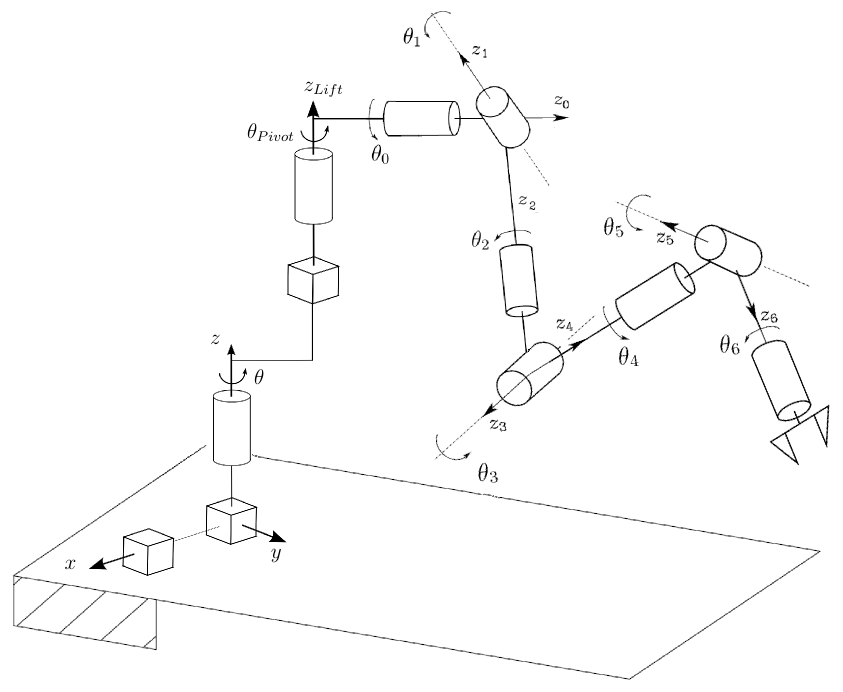
\includegraphics[width=.6\linewidth]{pictures/kinematic chain.png}
    \caption{Ejemplo de cadena cinemática \cite{noauthor_figure_nodate}.}
    \label{fig:chains}
\end{figure}

Tal y como se puede apreciar en la figura \ref{fig:chains}, las articulaciones pueden rotar y permiten la movilidad de cada uno de los segmentos del manipulador. Dado que estas articulaciones rotan, su posición se expresa numéricamente mediante unidades angulares. El concepto de cadena cinemática hace referencia a que, dado que cada una de las articulaciones esta unida a la siguiente mediante un segmento, se genera una cadena de movimientos en la que la posición espacial de cada una de las articulaciones se ve afectada por la posición angular de las anteriores.

Aplicando este principio, el modelo cinemático expresa matemáticamente la posición cartesiana del extremo del robot en función de las coordenadas angulares de las articulaciones. Existen pues dos perspectivas del modelo cinemático:

\begin{itemize}
    \item El modelo de cinemática directa expresa la posición espacial del extremo del manipulador en función de las coordenadas angulares de las articulaciones.
    \item El modelo de cinemática inversa expresa las coordenadas angulares de las articulaciones en función de las coordenadas cartesianas del extremo del manipulador.
\end{itemize}

\begin{figure}[H]
    \centering 
    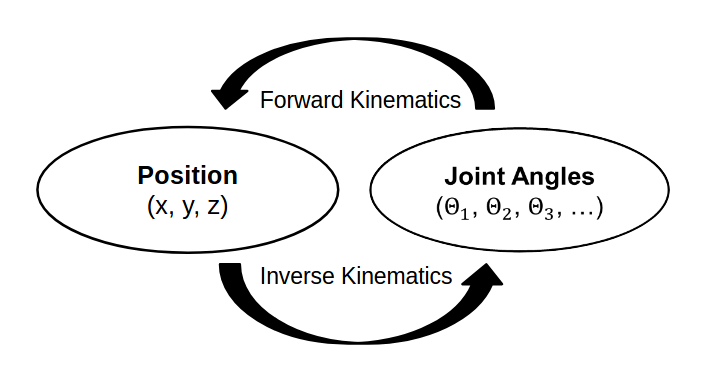
\includegraphics[width=.6\linewidth]{pictures/Kinematic Diagram.png}
    \caption{Diagrama del modelo cinemático \cite{noauthor_roboy_nodate}.}
    \label{fig:kdiagram}
\end{figure}

En conclusión, el modelo matemático conforma la base teórica y formal que permite realizar el estudio de los movimientos del manipulador y es por ello que representa un bloque crucial dentro del proyecto.



\section{\textit{Hardware}}
Los elementos \textit{hardware} conforman la implementación física del manipulador y de todos los componentes empleados para controlarlo.

En términos generales, el \textit{hardware} usado en el proyecto se descompone en diferentes elementos:
\begin{itemize}
    \item Impresión 3D de la estructura física del manipulador.
    \item Motores empleados en el manipulador.
    \item Desarrollo de la placa de circuito impreso de control y microcontrolador empleado.
    \item Comunicaciones entre los diferentes subsistemas.
\end{itemize}

En primer lugar, la impresión 3D es la tecnología seleccionada para la fabricación de la estructura física del manipulador debido a su bajo coste y accesibilidad. Esta parte del proyecto se centra en llevar a cabo la fabricación y construcción de la estructura física del manipulador, así como su ensamblado y testeo. Este apartado se ubica en el apartado 5.1 de la memoria.

En segundo lugar, la elección de los motores que dotan de movilidad a la estructura es una decisión crucial y que depende principalmente de cuales sean las características físicas del manipulador, así como de las tareas que se quieran realizar con el mismo. Existen numerosas opciones en cuanto a motores, por ejemplo, motores DC, servomotores, motores paso a paso, etc. Este apartado se ubica en el apartado \ref{sec:motors} de la memoria.

En tercer lugar, el desarrollo de la PCB de control y elección del microcontrolador representan la parte más importante dentro del bloque hardware del proyecto. El objetivo principal de esta parte del proyecto es llevar a cabo el diseño y construcción de una PCB personalizada, adaptada especialmente a los actuadores y microcontrolador usados para llevar a cabo el control del movimiento del manipulador. Se considera que esta PCB representa uno de los elementos hardware esenciales para el correcto desarrollo del proyecto. Este apartado se ubica en el apartado 5.3 de la memoria.

En último lugar, el diseño e implementación de los canales de comunicación y protocolos necesarios para comunicar los dos subsistemas principales requiere desarrollo hardware y software de forma equitativa, además, también representa uno de los elementos cruciales del proyecto. Este apartado se ubica en el apartado 5.4 de la memoria.





\section{\textit{Software}}
Los elementos software del proyecto abordan los siguientes aspectos:
\begin{itemize}
    \item Desarrollo de la aplicación de control del brazo robótico, implementada mediante una interfaz gráfica de usuario para garantizar su accesibilidad y facilidad de uso. Esta implementación se lleva a cabo en S1.
    \item Programación del microcontrolador e implementación del modelo matemático en la práctica con el objetivo de controlar los movimientos del brazo robótico. Esta implementación se lleva a cabo en S2.
\end{itemize}

En primer lugar, mediante el desarrollo de la aplicación de usuario se busca ofrecer una forma de controlar los movimientos del robot de forma fácil y accesible, para ello se ha desarrollado una interfaz de usuario que se ejecuta en un ordenador auxiliar. Desde esta aplicación el usuario puede controlar los movimientos del robot, además de monitorizar el estado del mismo. Las órdenes dadas por el usuario desde esta aplicación son enviadas al microcontrolador para su realización mediante los canales de comunicación mencionados anteriormente. Este desarrollo se ha llevado a cabo mediante el lenguaje  de programación Python. Este apartado se ubica en el apartado 6.1 de la memoria.

En segundo lugar, la programación del microcontrolador representa una parte esencial del proyecto, ya que toda la lógica de funcionamiento y control de los actuadores del brazo robótico se lleva a cabo en el mismo. Es por ello que la labor principal del microcontrolador es orquestar el funcionamiento de los actuadores, así como de realizar el computo necesario para transformar las ordenes del usuario en movimientos consecuentes del brazo robótico. La programación del microcontrolador se ha llevado a cabo mediante el lenguaje C. Este apartado se ubica en el apartado 6.2 de la memoria.


\chapter{Especificación de requisitos}
Copiar requisitos aqui para hacer Jutsu de + 10 paginas de memoria
\chapter{Diagramas y diseño}
Una parte importante de un proyecto integral de ingeniería es la elicitación de requisitos y la creación de diagramas que representen el sistema de manera abstracta en base a dichos requisitos.

El sistema de gobierno del p-Arm esta compuesto de dos subsistema al ser necesaria tanto una placa de control como un ordenador auxiliar desde el cual un operario humano pueda interactuar con el brazo. El software del sistema de control del ordenador será representado mediante un diagrama de clases mientras que el software que ira cargado en la placa de control será representado por un diagrama de bloques general y varios diagramas de estados que detallarán el comportamiento del sistema.

Para realizar dichos diagramas se ha empleado Papyrus, una herramienta de edición gráfica para realización de diagramas. Para modelizar los diagramas del sistema de control que ira en el ordenador auxiliar se ha empleado el estándar UML2 definido por la OMG, por otro lado, para realizar los diagramas del software que será cargado en la placa de control se ha empleado el estándar SysUML 1.4 ya que permite mejor representación del sistema empotrado.

A continuación se pueden observar los requisitos que el equipo de desarrollo ha elicitado además de una explicación de los diagramas que representan los dos subsistemas que componen el proyecto,




En base a los anteriores requisitos el grupo de desarrollo ha generado los siguientes diagramas para el software de la placa de control.

\begin{figure}[H]
    \centering
    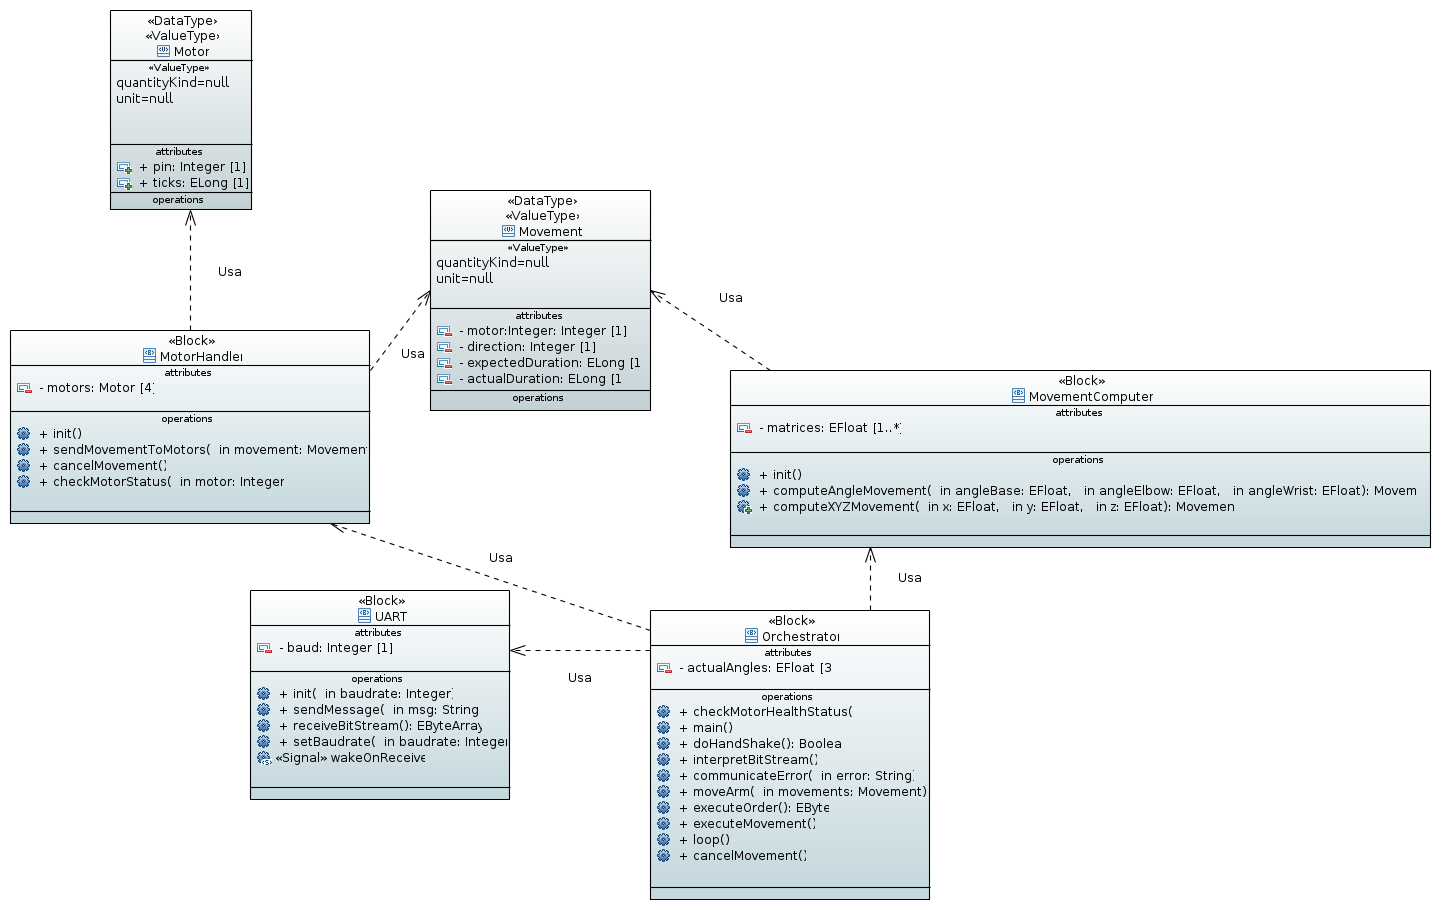
\includegraphics[width=\linewidth]{pictures/S2BlockDiagram.PNG}
    \caption{Diagrama de bloques del \ac{S2}}
    \label{fig:diagrama_bloques_s2}
\end{figure}

En el diagrama \ref{fig:diagrama_bloques_s2} se pueden observar los bloques que componen el \ac{S2} además de dos tipos de datos los cuales han sido creados para facilitar el control de los motores del brazo.

A continuación se explican cada uno de los bloques:

\begin{itemize}
    \item \texttt{MotorHandler}: este bloque es capaz de controlar los motores de manera directa empleando el tipo de dato ``\texttt{Movement}'' enviando la señal necesaria para realizar el movimiento requerido. Además permite verificar el estado de los motores y cancelar los movimientos si esto fuese necesario.
    
    \item \texttt{UART}: este bloque es el encargado de la comunicación asíncrona entre el \ac{S1} y el \ac{S2}. Controla el ratio de baudios de la comunicación y realiza la transmisión y la recepción de información hasta y desde el \ac{S1}. A través de este bloque se reciben las ordenes procedentes del \ac{S1} y se envían los errores y la posición del brazo al S1 desde el \ac{S2}.
    
    \item \texttt{Orchestrator}: encargado de coordinar los demás bloques. En el se encuentra la lógica principal del \ac{S2}. Algunas de sus funciones mas importantes son interpretar el flujo de bits que llega desde el S1 para obtener una orden concreta; ordenar el movimiento del brazo empleando los demás bloques o hacer el ``hadshake'' inicial entre el \ac{S1} y el \ac{S2}. Posteriormente se entrará mas en detalle en el comportamiento de este bloque al analizar los diagramas de estados.
    
    \item \texttt{MovementComputer}: se encarga de computar el movimiento que se tendrá que comunicar a los motores. Para ello deberá obtener las posiciones deseadas gracias al bloque UART y al ``\texttt{Orchestrator}''.
\end{itemize}

A continuación se explican las dos estructuras de datos que se aprecian en el diagrama \ref{fig:diagrama_bloques_s2}

\begin{itemize}
    \item Motor: Este tipo de dato es empleado por el ``MotorHandler'' para saber a que pin debe mandar la señal ``PWM'' que gobierna los motores y durante cuantos ticks deberá estar activa dicha señal
    
    \item Movement: El ``MovementComputer'' genera un array de 3 posiciones de este tipo de dato, uno por cada motor de giro del brazo. El atributo ``moto'' guarda un integer que representa uno de los motores del brazo; ``direction'' sirve para conocer la dirección de giro de dicho motor; ``expectedDuration'' guarda la duración  
\end{itemize}

A continuación se explican los diagramas de estados de cada uno de los métodos que aparecen en el diagrama de bloques general.

En el caso del ``Orchestrator'' tenemos los siguientes diagramas.

\begin{figure}[H]
    \centering
    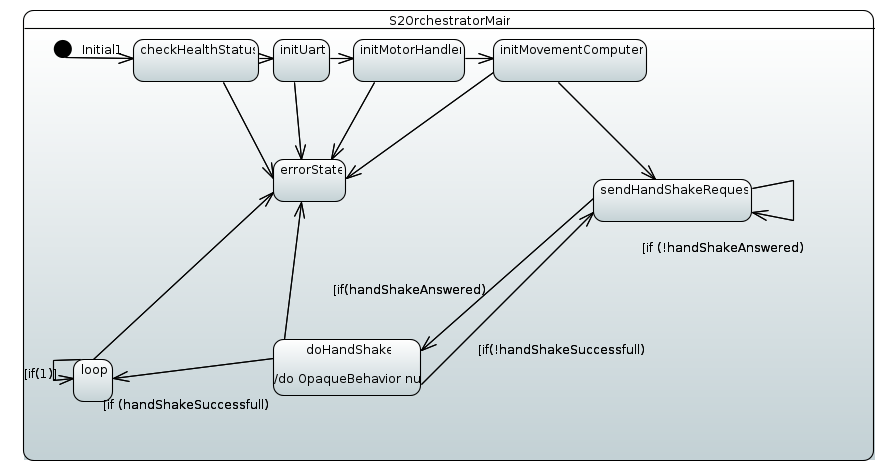
\includegraphics[width=1\linewidth]{pictures/S2OrchestratorMain.PNG}
    \caption{Diagrama de estados del método \texttt{main()} del \textit{orchestrator}.}
    \label{fig:fun_main_orchestrator}
\end{figure}

Este método solo se ejecutará una vez, en cuanto el sistema se ponga en marcha. 

\begin{itemize}
    \item \texttt{checkHealthStatus}: Se verifica la situación de los componentes del brazo robótico para confirmar que todos están en un astado adecuado para el funcionamiento. 
    \item \texttt{initUart}: Se inicializa la UART definiendo un ratio de baudios concreto.
    \item \texttt{initMotorHandler}: Se inicializa el controlador de los motores.
    \item \texttt{initMovementComputer}: Se inicializa el computador de movimientos.
    \item \texttt{sendHandShakeRequest} : Se manda una petición de handshake para verificar si hay algún ordenador conectado. Si se detecta alguno se pasa al siguiente estado, si no, se mantiene en ese estado mandando requests.
    \item \texttt{doHandShake}: Si en el estado anterior se detecta un ordenador se pasa a este estado. Se realiza una serie de intercambios de información para verificar que el ordenador conectado es adecuado para el control del brazo.
    \item \texttt{loop}: Se pasa al bucle de funcionamiento si el handshake ha sido correcto.
    \item \texttt{errorState}: Estado de error al que se llega si en alguno de los estados ocurre algún problema inesperado. 
    
    
\end{itemize}

\begin{figure}[H]
    \centering
    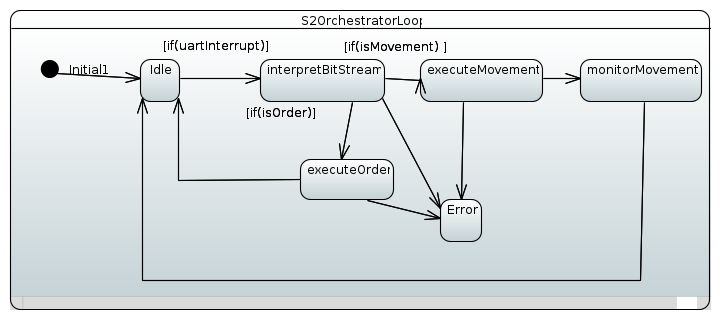
\includegraphics[width=1\linewidth]{pictures/S2OrchestratorLoop.PNG}
    \caption{Diagrama de estados del método \texttt{loop()} del \textit{orchestrator}.}
    \label{fig:fun_loop_orchestrator}
\end{figure}

Este método es el bucle principal del brazo robotico. Tras ejecutar \texttt{main()} el sistema entrará en este bucle y no saldrá hasta que se apaga.

\begin{itemize}
    \item \texttt{Idle}: el brazo se encuentra ocioso y a la espera de una orden desde el \ac{S1}
    \item \texttt{interpretBitStream}: tras una interrupción de la UART el \ac{S2} entiende que hay una orden o movimiento procedentes del \ac{S1} y se avanza a este estado. El bitStream es interpretado para saber si es una orden o un movimiento.
    \item \texttt{executeMovement}: si tras interpretar el bitStream resulta que es un movimiento, el sistema avanza a este estado y se ponen en marcha los demás bloques para poder generar un movimiento en los motores en base a la posición recibida desde \ac{S1}
    \item \texttt{executeOrder}: si tras interpretar el bitStream resulta que es una orden, el sistema avanza a este estado y se ponen en marcha los bloques necesarios para ejecutar dicha orden.
    \item \texttt{monitorMovement} : tras empezar a ejecutar un movimiento el brazo empieza a monitorizarlo para poder determinar cuando se ha terminado o, si es cancelado, actualizar la posición en la que se ha quedado el brazo.
    \item \texttt{errorState}: Estado de error al que se llega si en alguno de los estados ocurre algún problema inesperado. 
    
    
\end{itemize}

\begin{figure}[H]
    \centering
    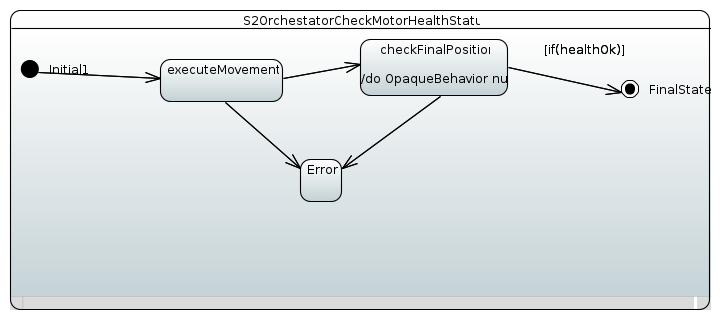
\includegraphics[width=1\linewidth]{pictures/S2OrchestratorCheckMotorHealthStatus.PNG}
    \caption{Diagrama de estados del método \texttt{CheckMotorHealthStatus()} del \textit{orchestrator}.}
    \label{fig:fun_check_motor_health_status_orchestrator}
\end{figure}

Este método comprueba el estado de los motores para asegurar que estos tienen un funcionamiento correcto antes de recibir cualquier orden de movimiento.

\begin{itemize}
    \item \texttt{executeMovement}: se ejecuta un movimiento a una posición en la que todos los fines de carrera sean activados.
    \item \texttt{interpretBitStream}: se verifica que todos los fines de carrera han sido alcanzados pudiendo concluir que el brazo es capaz de mover todos sus motores.
    
\end{itemize}

\begin{figure}[H]
    \centering
    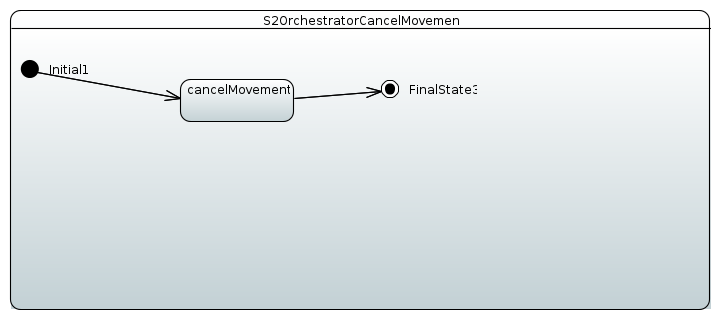
\includegraphics[width=1\linewidth]{pictures/S2OrchestratorCancelMovement.PNG}
    \caption{Diagrama de estados del método \texttt{CancelMovement()} del \textit{orchestrator}.}
    \label{fig:fun_cancel_movement_orchestrator}
\end{figure}

Este método finaliza un movimiento que se este realizando.

\begin{itemize}
    \item \texttt{cancelMovment}: se cancela el movimiento y se guarda la posición actual del brazo..
    
\end{itemize}

\begin{figure}[H]
    \centering
    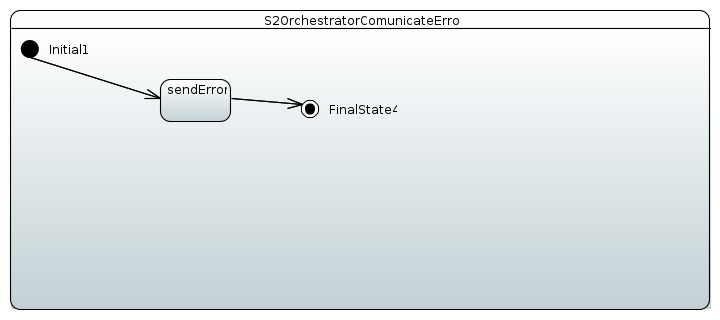
\includegraphics[width=1\linewidth]{pictures/S2OrchestratorComunicateError.PNG}
    \caption{Diagrama de estados del método \texttt{ComunicateError()} del \textit{orchestrator}.}
    \label{fig:fun_comunicate_error_orchestrator}
\end{figure}

Este método comunica un error al \ac{S1}.

\begin{itemize}
    \item \texttt{cancelMovment}: se envía un bitStream que representa un error ocurrido en el \ac{S2}
    
\end{itemize}

\begin{figure}[H]
    \centering
    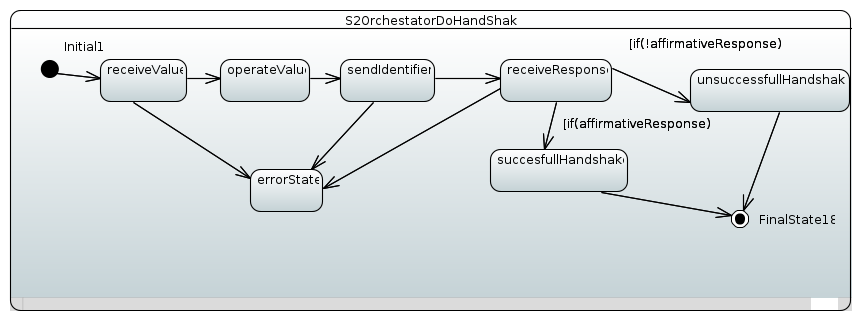
\includegraphics[width=1\linewidth]{pictures/S2OrchestratorDoHandShake.PNG}
    \caption{Diagrama de estados del método \texttt{DoHandShake()} del \textit{orchestrator}.}
    \label{fig:fun_do_hand_shake_orchestrator}
\end{figure}

Este método es el encargado de autenticar a los dispositivos entre si y configurar un canal para su posterior comunicación

\begin{itemize}
    \item \texttt{receiveValue}: se realizan los procedimientos necesarios para recibir un valor desde \ac{S1} a través de la \ac{UART}.
    \item \texttt{operateValue}: se realiza una operación matemática con el valor recibido para generar de esta manera un identificador.
    \item \texttt{sendIdentifier}: se envía dicho identificador de vuelta a \ac{S1}.
    \item \texttt{receiveResponse}: se recibe la respuesta de ac{S1} para saber si el \ac{hand--shake} ha sido realizado con éxito.
    \item \texttt{succesfulHandshake}: en caso de que en el estado
    \texttt{receiveResponse} se haya recibido una respuesta afirmativa se pasa a este estado que representa que el dispositivo que conforma S1 y S2 han conseguido autenticarse entre si.
    \item \texttt{unsuccesfulHandshake}: en caso de que en el estado\texttt{receiveResponse} se haya recibido una respuesta negativa se pasa a este estado que representa que el dispositivo que conforma S1 y S2 no han conseguido autenticarse
    entre si.
    \item \texttt{errorState}: Estado de error al que se llega si en alguno de los estados ocurre algún problema inesperado. 
\end{itemize}

\begin{figure}[H]
    \centering
    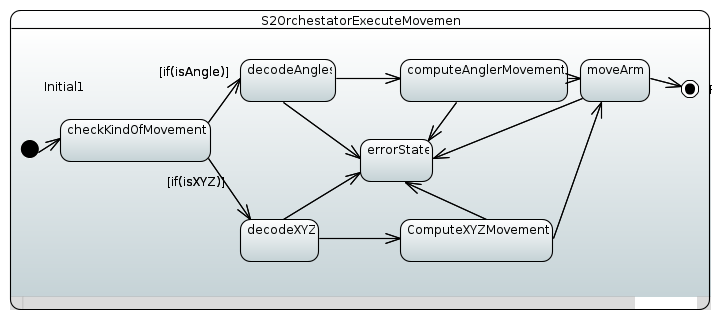
\includegraphics[width=1\linewidth]{pictures/S2OrchestratorExecuteMovement.PNG}
    \caption{Diagrama de estados del método \texttt{ExecuteMovement()} del \textit{orchestrator}.}
    \label{fig:fun_execute_movement_orchestrator}
\end{figure}

Este método es el encargado de, una vez recibida la trama de bits que representa movimiento desde el S1, decidir si el movimiento ha sido representado como ángulos o posiciones cartesianas y posteriormente ordenar las operaciones necesarias para que se generen las señales PWM que moveran los motores.

\begin{itemize}
    \item \texttt{checkKindOfMovement}: Se verifica si el movimiento ha sido transmitido como una posición cartesiana o como unos ángulos destino para los motores y se procede en consecuencia.
    \item \texttt{decodeAngles}: En caso de que fueran ángulos, se transita a este estado. Se interpreta la trama de bits y se obtiene el valor numérico de los ángulos.
    \item \texttt{computeAngleMovement}: Se realizan comprobaciones para verificar que los ángulos están dentro de los limites del brazo y se procede a generar el array de movimientos que se necesitan hacer para conseguir llegar desde la posición actual a la posición destino.
    \item \texttt{decodeXYZ}: En caso de que fueran posiciones cartesianas se transita a este estado. Se interpreta la trama de bits y se obtienen las coordenadas en centímetros.
    \item \texttt{computeXYZMovements}: Para simplificar los cálculos matemáticos posteriores las posiciones cartesianas se convierten en ángulos. Se verifica si los ángulos están dentro de los limites del brazo y se procede a generar el \textit{array} de movimientos que se necesitan hacer para conseguir llegar desde la posición actual a la posición destino.
    \item \texttt{moveArm}: Se envían los movimientos a los motores.
    \item \texttt{errorState}: Estado de error al que se llega si en alguno de los estados ocurre algún problema inesperado. 
    
\end{itemize}

\begin{figure}[H]
    \centering
    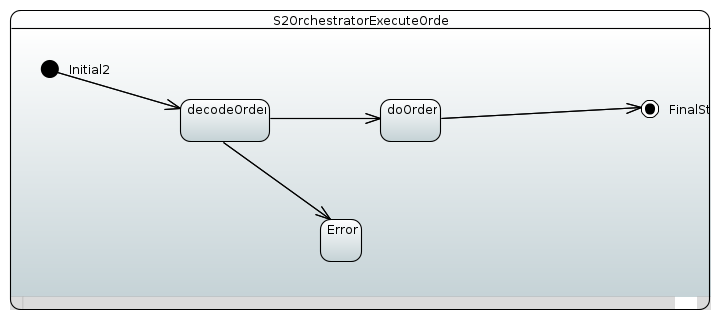
\includegraphics[width=1\linewidth]{pictures/S2OrchestratorExecuteOrder.PNG}
    \caption{Diagrama de estados del método \texttt{ExecuteOrder()} del \textit{orchestrator}.}
    \label{fig:fun_execute_order_orchestator}
\end{figure}

Este método es el encargado de, una vez recibida la trama de bits que representa una orden distinta de realizar un movimiento desde el S1, decodificar dicha orden y realizarla.

\begin{itemize}
    \item \texttt{decodeOrder}: Se interpreta la trama de bits para obtener la orden proveniente desde S1.
    \item \texttt{doOrder}: Se ejecuta la orden obtenida en el estado anterior.
    \item \texttt{Error}: Estado de error al que se llega si en alguno de los estados ocurre algún problema inesperado. 
\end{itemize}

\begin{figure}[H]
    \centering
    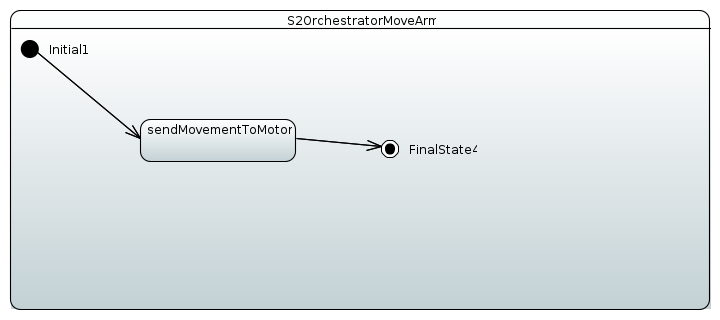
\includegraphics[width=1\linewidth]{pictures/S2OrchestratorMoveArm.PNG}
    \caption{Diagrama de estados del método \texttt{moveArm()} del \textit{orchestrator}.}
    \label{fig:fun_move_arm_orchestator}
\end{figure}

Este método es el encargado de mandar los movimientos a los motores una vez estos se hayan computado.

\begin{itemize}
    \item \texttt{sendMovementToMotors}: se mandan los movimientos necesarios a los motores.
    
\end{itemize}

En el caso del bloque “UART” tenemos los siguientes diagramas.

\begin{figure}[H]
    \centering
    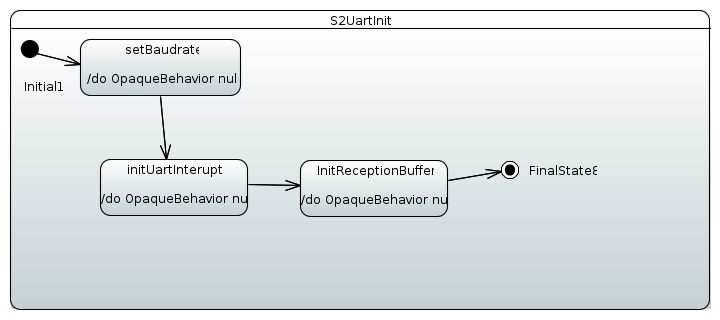
\includegraphics[width=1\linewidth]{pictures/S2UartInit.PNG}
    \caption{Diagrama de estados del método \texttt{uartInit()} del \textit{UART}.}
    \label{fig:fun_uart_init_uart}
\end{figure}

Se ejecuta este método al inicio de la comunicación a través de la UART para configurar la transmisión de datos.

\begin{itemize}
    \item \texttt{setBaudrate}: Se establece el ratio de baudios para la transmisión asíncrona
    \item \texttt{initUartInterupt}: Se configura el registro de interrupciones de tal manera que la UART sea capaz de generar una interrupción en el sistema con el objetivo de poder saber cuando se ha recibido una nueva trama de bits.
    \item \texttt{initReceptionBuffer}: Se inicializa el \textit{buffer} de recepción.
    
\end{itemize}

\begin{figure}[H]
    \centering
    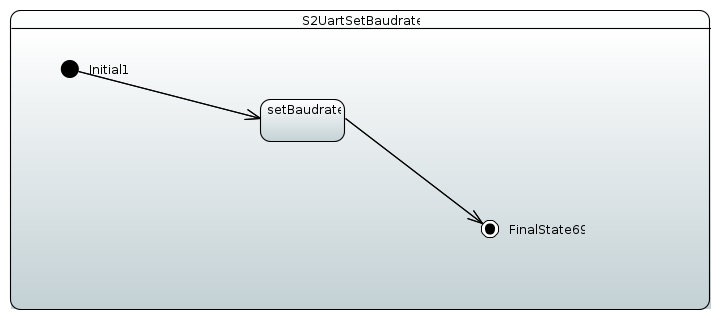
\includegraphics[width=1\linewidth]{pictures/S2UartSetBaudrate.PNG}
    \caption{Diagrama de estados del método \texttt{setBaudrate()} del \textit{UART}.}
    \label{fig:fun_set_baudrate_uart}
\end{figure}

Se configuran los registros necesarios para obtener un ratio de baudios adecuados para la comunicación

\begin{itemize}
    \item \texttt{setBaudrate}: Se realiza la configuración 
\end{itemize}

\begin{figure}[H]
    \centering
    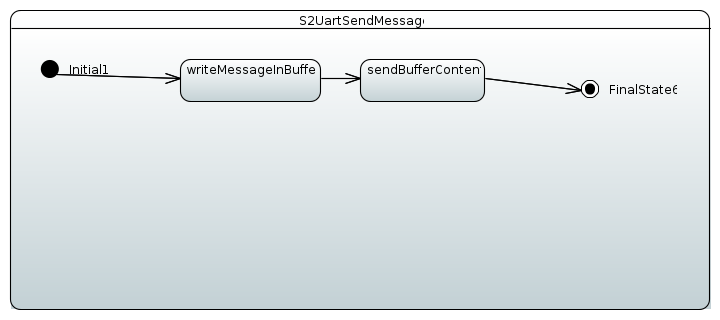
\includegraphics[width=1\linewidth]{pictures/S2UartSendMessage.PNG}
    \caption{Diagrama de estados del método \texttt{sendMessage()} del \textit{UART}.}
    \label{fig:fun_send_message_uart}
\end{figure}

Se escribe un mensaje en el \textit{buffer} de envio y este es posteriormente enviado.

\begin{itemize}
    \item \texttt{writeMessageInBuffer}: Se escribe el mensaje en el \textit{buffer} de salida de la UART.
    \item \texttt{sendBufferContent}: Se envía el contenido del buffer al \ac{S1}
\end{itemize}

\begin{figure}[H]
    \centering
    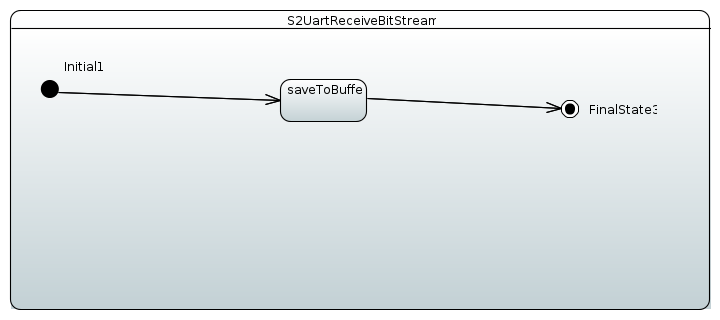
\includegraphics[width=1\linewidth]{pictures/S2UartReceiveBitStream.PNG}
    \caption{Diagrama de estados del método \texttt{receiveBitStream()} del \textit{UART}.}
    \label{fig:fun_receive_bit_stream_uart}
\end{figure}

Se guarda un mensaje en el \textit{buffer} de recepción.

\begin{itemize}
    \item \texttt{saveToBuffer}: Se escribe el mensaje en el \textit{buffer} de entrada de la UART.
\end{itemize}





%% REVISADO - J
\chapter{Fundamentos matemáticos del proyecto}
\label{chap:maths}
En este proyecto el soporte matemático tiene una importancia destacada. Es por ello que se han tenido que superar retos como: el movimiento de los motores de forma coordinada para alcanzar
diversas posiciones a lo largo del rango de movilidad del brazo.

La relación entre los ángulos de los ejes y el punto final del brazo no es trivial y 
es necesario un estudio previo de distintos factores para poder hacerlo correctamente. 
Por una parte, es necesario definir de la manera más precisa posible la configuración 
geométrica del brazo. Dicha configuración relaciona los distintos segmentos que
conforman el manipulador según una convención de parámetros
que trabaja sobre las posibles articulaciones que componen el brazo robótico 
y que se denotan por $Z_i$, donde $i$ es el número de la articulación.

En particular, las relaciones a estudiar son:

\begin{itemize}
    \item El ángulo presente entre dos articulaciones adyacentes
          $\widehat{Z_aZ_b}~rad$, el cual se denota por `$\alpha_b$'.
    \item La distancia presente entre dos articulaciones adyacentes
          $\overline{Z_aZ_b}$, representada por `$a_b$'.
    \item El sentido de la rotación de una articulación,
          $\overrightarrow{X_aY_a}$, denotada por `$\theta_a$'.
\end{itemize}

Estas relaciones permiten establecer la configuración geométrica del robot,
fundamental para poder definir los movimientos posibles del mismo y generar tanto
las matrices de la cinemática directa como obtener las ecuaciones de la cinemática
inversa. Además, se puede obtener de la misma manera las matrices Jacobianas que
permiten conseguir datos útiles como el trabajo, la velocidad o la potencia.

Para el $\mu$Arm, se obtuvieron las siguientes configuraciones geométricas:

\begin{figure}[H]
    \centering
    \begin{minipage}{.4\linewidth}
        \centering
        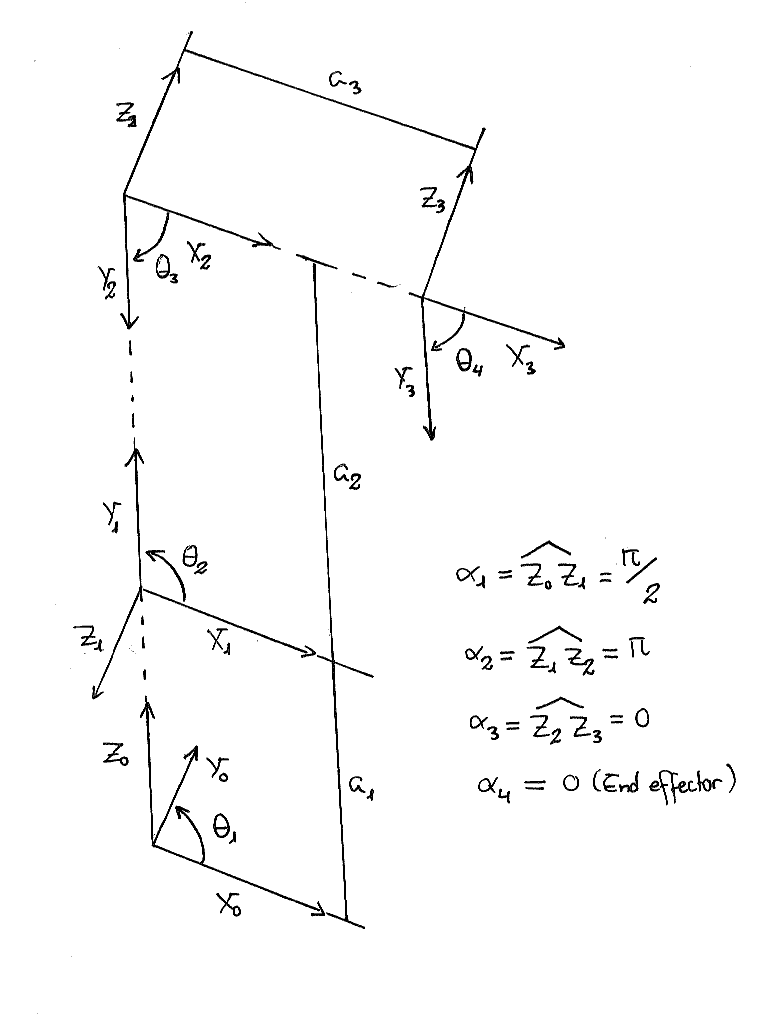
\includegraphics[width=\textwidth]{pictures/geometric_configuration_2.png}
        \caption{Configuración geométrica del $\mu$Arm.}
        \label{fig:uArm_gc}
    \end{minipage}
    \hfill
    \begin{minipage}{.48\linewidth}
        \centering
        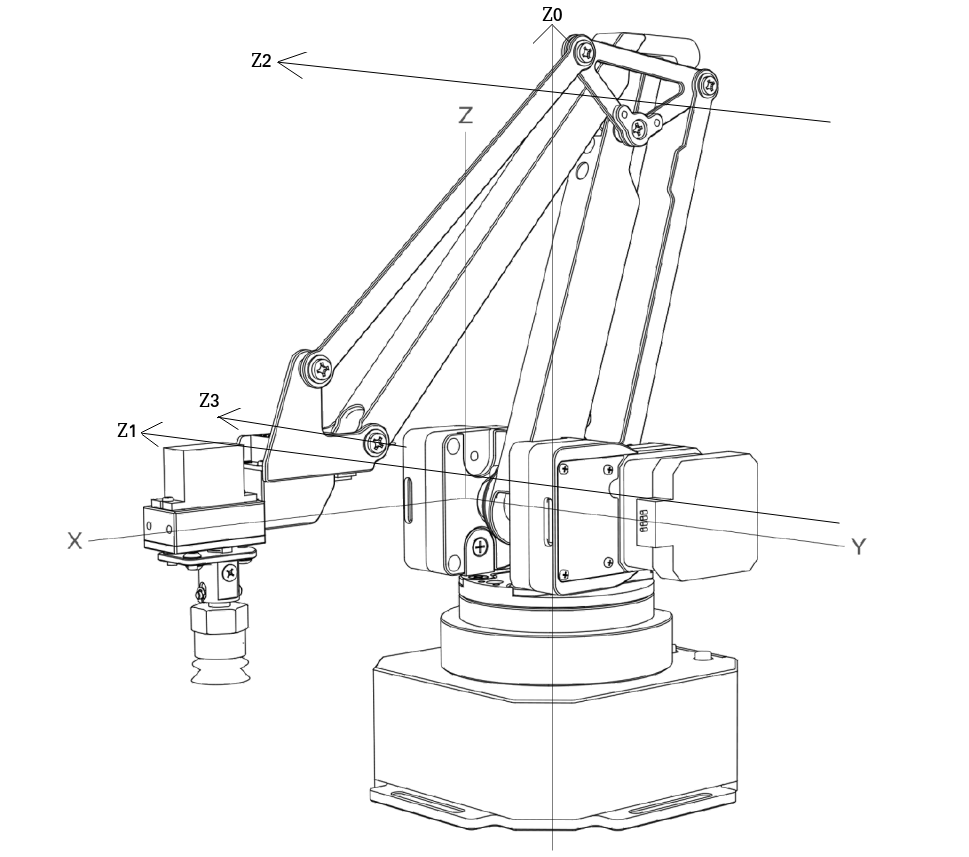
\includegraphics[width=\textwidth]{pictures/axis.png}
        \caption{Los distintos grados de libertad del $\mu$Arm, representados por $Z_i$.}
        \label{fig:uArm_axis}
    \end{minipage}
\end{figure}

Con estos valores, ya se pueden obtener las distancias entre articulaciones así
como las desviaciones entre las mismas, si las hay. En el caso particular del $\mu$Arm,
se obtiene unos datos como los siguientes (las medidas se han obtenido desde la guía del
desarrollador de UFACTORY\cite{ufactoryUArmSwiftPro2017}):

\begin{table}[ht]
    \begin{minipage}{.49\linewidth}
        \begin{figure}[H]
            \centering
            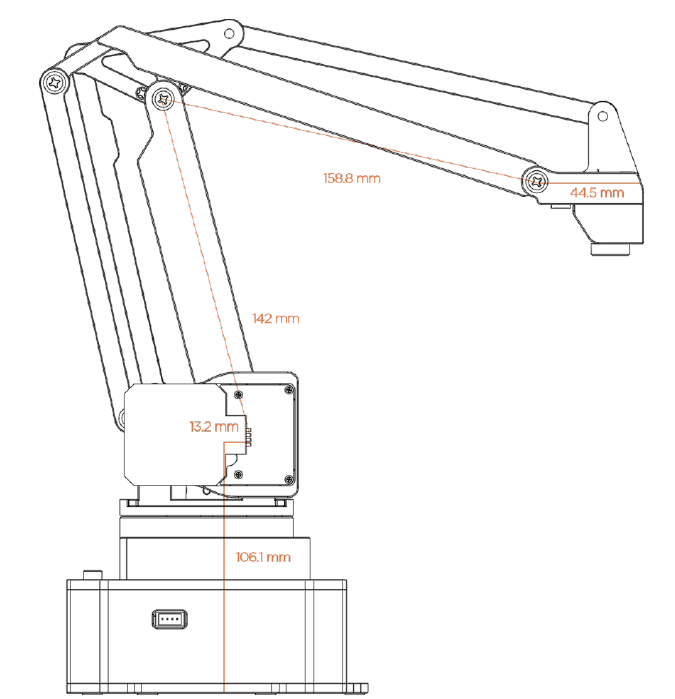
\includegraphics[width=\linewidth]{pictures/sizes.png}
            \caption{Longitudes del brazo robótico \cite{ufactoryUArmSwiftPro2017}.}
            \label{fig:sizes}
        \end{figure}
    \end{minipage}
    \hfill
    \begin{minipage}{.49\linewidth}
        \centering
        \begin{tabular}{|| c | c c ||}
            \hline
            $i$ & $a_i~(mm.)$ & $d_i~(mm.)$ \\ [0.5ex]
            \hline\hline
            $1$ & $13.2$      & $106.1$     \\
            \hline
            $2$ & $142$       & $0$         \\
            \hline
            $3$ & $158.8$     & $0$         \\
            \hline
            $4$ & $44.5$      & $0$         \\ [1ex]
            \hline
        \end{tabular}
        \caption{Longitudes y desviaciones del manipulador $\mu$Arm.}
        \label{tab:uArm-ld-values}
    \end{minipage}
\end{table}

Esta información permite construir una tabla de \textit{Denavit--Hartenberg} que
recoge la información del robot. Dicha tabla se conoce también como ``parámetros de
\textit{Denavit--Hartenberg}'', que conforman cuatro variables que recogen, en una
convención particular, la referencia de una cadena cinemática (objetos rígidos unidos
a articulaciones que responden a una función matemática) o de un brazo robótico \cite{DenavitHartenbergParameters2020}.

La convención de parámetros de \textit{Denavit--Hartenberg} son los siguientes:
\begin{itemize}
    \item $d$ -- desviación a lo largo del eje $Z$ respecto a la normal común\footnote{la normal
              común de dos articulaciones que no intersecan se define como la línea perpendicular a
              ambos ejes, que se usa comúnmente para conocer la separación entre ambas dos \cite{CommonNormalRobotics2017}.}
          con el ángulo anterior.
    \item $\theta$ -- el ángulo de rotación desde $x_i$ hasta $y_i$. Sirve para definir
          el sentido del mismo además de indicar el movimiento que realiza dicha articulación.
    \item $a$ -- la distancia respecto a la normal común entre dos articulaciones $\left(\overline{Z_{i - 1}Z_i}\right)$.
    \item $\alpha$ -- el ángulo sobre la normal común, en este caso, desde $Z_{i - 1}$ hacia $Z_i$ $\left(\widehat{Z_aZ_b}\right)$.
\end{itemize}

Esta convención es especialmente interesante porque permite definir de forma precisa
las relaciones entre las articulaciones, pudiendo conocer la rotación relativa entre
dos de ellas y la traslación entre sus puntos. Además, aplicando las propiedades
de las matrices, se puede obtener la relación absoluta entre las rotaciones y las
traslaciones, lo que se traduce en conocer el punto exacto $\left\{x, y, z\right\}$ en el que se encuentra el
\textit{end--effector} cuando se giran las articulaciones
$\left\{\theta_0, \theta_1, \cdots, \theta_i\right\}~rad$ respectivamente.

Esta relación se representa mediante una matriz, definida en la ecuación \ref{eq:dh-matrix}:

\begin{equation}
    \label{eq:dh-matrix}
    {
    \displaystyle \operatorname {}
    ^{i-1}T_{i}=\left[{
                \begin{array}{ccc|c}
                    \cos{\theta_{i}} & -\sin{\theta_{i}}\cos{\alpha_{i}} & \sin{\theta_{i}}\sin{\alpha_{i}}  & d_{i}\cos{\theta_{i}} \\
                    \sin{\theta_{i}} & \cos{\theta_{i}}\cos{\alpha_{i}}  & -\cos{\theta_{i}}\sin{\alpha_{i}} & d_{i}\sin{\theta_{i}} \\
                    0                & \sin{\alpha_{i}}                  & \cos{\alpha_{i}}                  & d_{i}                 \\
                    \hline
                    0                & 0                                 & 0                                 & 1
                \end{array}}\right] =
    \left[{
                \begin{array}{ccc|c}
                      &   &   &   \\
                      & R' &   & T' \\
                      &   &   &   \\
                    \hline
                    0 & 0 & 0 & 1
                \end{array}}
        \right]
    }
\end{equation}

donde $R'$ representa la \textit{rotación relativa} y $T'$ la \textit{traslación relativa}.

Otra ventaja de los parámetros de \textit{Denavit--Hartenberg} es la posibilidad de
definir elementos cinemáticos\footnotemark[2], como la velocidad $\left(W_{i,j}(k)\right)$ y la aceleración ($H_{i,j}(k)$)
de distintos cuerpos así como elementos dinámicos tales como la inercia $\left(J\right)$,
el momento lineal y angular $\left(\Gamma\right)$ o las fuerzas y torques aplicados
$\left(\Phi\right)$ \footnote{si bien estos datos resultan muy útiles, para el proyecto no se consideran
    necesariamente relevantes, ya que están supeditados a la velocidad y a la masa (cuanto mayores sean,
    la aplicación de dichos elementos cinemáticos será mayor sobre los componentes del
    manipulador), y el brazo robótico no presenta ni una masa suficientemente elevada ni alcanza velocidades altas
    como para afectar en gran media al comportamiento del mismo, pero sí se contempla realizar un estudio para completar
    este proyecto en una futura versión.}.

Para un manipulador basado estructuralmente en el $\mu$Arm, se obtienen unos parámetros
de \textit{Denavit--Hartenberg} como los mostrados en la tabla \ref{tab:dh-params-with-phi}:

\begin{table}[H]
    \centering
    \begin{tabular}{ c | c c c c }
        $i$ & $\theta_i$ & $d_i~(mm.)$ & $a_i~(mm.)$ & $\alpha_i$          \\ [0.5ex]
        \hline
        $1$ & $\theta_1$ & $a_1$       & $d_1$       & $\nicefrac{\pi}{2}$ \\
        $2$ & $\theta_2$ & $0$         & $a_2$       & $\pi$               \\
        $3$ & $\theta_3$ & $0$         & $a_3$       & $0$                 \\
        $4$ & $\theta_4$ & $0$         & $a_4$       & $0$                 \\ [1ex]
    \end{tabular}
    \caption{Tabla inicial de \textit{Denavit–Hartenberg} para un manipulador basado en el $\mu$Arm parametrizada.}
    \label{tab:dh-params-with-phi}
\end{table}

En un estudio realizado previamente \cite{javieralonsosilvaEstudioManipuladorUArm2019},
se descubrió (en relación con las tablas \ref{tab:uArm-ld-values} y \ref{tab:dh-params}
y con el primer punto de la convención de los parámetros de \textit{Denavit--Hartenberg})
que la desviación `$d_1$' de la primera articulación estaba invertida con la distancia de la normal común
`$a_1$' ya que, como se puede ver en dicho primer punto, la desviación es sobre el eje $Z$.
Por ello, en la tabla \ref{tab:uArm-ld-values} los valores de `$a_1$' y `$d_1$' están
intercambiados. Además, también se vio que este tipo de estructuras pantográficas
tienen su \textit{end--effector} siempre paralelo al plano del suelo (equivalente
a que el ángulo con el plano $X$ es $\phi_e = \pi$), por lo que el cuarto elemento de
los parámetros de \textit{Denavit--Hartenberg} para un manipulador basado en el $\mu$Arm
se puede obviar para luego añadirlo como una traslación en el eje $Z$ $\left(T_Z\right)$,
quedando como se muestra en la tabla \ref{tab:dh-params}:

\begin{table}[H]
    \centering
    \begin{tabular}{ c | c c c c }
        $i$ & $\theta_i$ & $d_i~(mm.)$ & $a_i~(mm.)$ & $\alpha_i$          \\ [0.5ex]
        \hline
        $1$ & $\theta_1$ & $a_1$       & $d_1$       & $\nicefrac{\pi}{2}$ \\
        $2$ & $\theta_2$ & $0$         & $a_2$       & $\pi$               \\
        $3$ & $\theta_3$ & $0$         & $a_3$       & $0$                 \\ [1ex]
    \end{tabular}
    \caption{Tabla de \textit{Denavit–Hartenberg} para un manipulador basado en el $\mu$Arm parametrizada.}
    \label{tab:dh-params}
\end{table}

Esta característica simplifica los cálculos del ángulo final ya que siempre es el mismo
$\left(\pi~rad\right)$, quedando únicamente por calcular los valores de $\theta_2$ y 
$\theta_3$.

Una vez obtenidos los datos correspondientes al robot, podemos definir múltiples 
relaciones entre los mismos:
\begin{itemize}
    \item La cinemática directa, la cual permite saber el punto $\left\{x, y, z\right\}$
          según unos ángulos $\left\{\theta_0, \theta_1, \theta_2\right\}$ de entrada.
    \item La cinemática inversa, que permite conocer qué ángulos 
          $\left\{\theta_0, \theta_1, \theta_2\right\}$ posicionan el robot en un punto
          $\left\{x, y, z\right\}$.
    \item La matriz Jacobiana, donde se puede obtener un movimiento $\overrightarrow{x}$ según 
          qué velocidad haya en las articulaciones $\overrightarrow{q}$.
    \item La matriz Jacobiana inversa, la cual devuelve el valor de la velocidad en
          las articulaciones $\overrightarrow{q}$ para generar un movimiento en el 
          \textit{end--effector} $\overrightarrow{x}$.
\end{itemize}

Dado que las cuatro relaciones anteriores son útiles para conocer y definir
el comportamiento del robot, se estudiarán todas ellas para ver cómo se pueden utilizar
en el manipulador.
\section{Cinemática directa}
La cinemática directa permite conocer la rotación relativa entre dos articulaciones
junto con la traslación relativa entre las mismas, utilizando para ello la matriz
definida en la ecuación \ref{eq:dh-matrix}.

Como se puede ver en dicha matriz, se relaciona una articulación $i$ con el equivalente
anterior, en este caso $i - 1$, obteniéndose así la rotación relativa $R'$ y la
traslación relativa $T'$. Si bien esta aproximación es sencilla, solo permite relacionar
dos articulaciones entre sí y que estén en principio unidas por la normal común.

En este brazo se disponen de tres articulaciones, como se muestra en la tabla
\ref{tab:dh-params}, por lo que interesa obtener la matriz $^{0}T_{3}$, la cual relaciona
directamente todas las articulaciones del brazo y permite obtener la rotación absoluta
$R$ y la traslación absoluta $T$.

La obtención de esta matriz es trivial y responde a la ecuación \ref{eq:t03}:

\begin{equation}
    \label{eq:t03}
    ^0T_3 = {^0T_1} \cdot {^1T_2} \cdot {^2T_3}
\end{equation}

Dada que la multiplicación de matrices ha de realizarse en cierto orden, los
factores han de permanecer en la misma posición siempre. De esta manera, se obtienen
las siguientes matrices intermedias (ecuaciones \ref{eq:t01}, \ref{eq:t12}, \ref{eq:t23})
y la matriz final (ecuación \ref{eq:t03-final}):

\begin{align}
    ^0T_1 & =
    \begin{bmatrix}
        \cos{\theta_{1}} & 0 & \sin{\theta_{1}}   & a_{1} \cos{\theta_{1}} \\
        \sin{\theta_{1}} & 0 & - \cos{\theta_{1}} & a_{1} \sin{\theta_{1}} \\
        0                & 1 & 0                  & d_{1}                  \\
        0                & 0 & 0                  & 1                      \\
    \end{bmatrix}\label{eq:t01} \\[1ex]
    ^1T_2 & =
    \begin{bmatrix}
        \cos{\theta_{2}} & \sin{\theta_{2}}   & 0  & a_{2} \cos{\theta_{2}} \\
        \sin{\theta_{2}} & - \cos{\theta_{2}} & 0  & a_{2} \sin{\theta_{2}} \\
        0                & 0                  & -1 & 0                      \\
        0                & 0                  & 0  & 1                      \\
    \end{bmatrix}\label{eq:t12} \\[1ex]
    ^2T_3 & =
    \begin{bmatrix}
        \cos{\theta_{3}} & - \sin{\theta_{3}} & 0 & a_{3} \cos{\theta_{3}} \\
        \sin{\theta_{3}} & \cos{\theta_{3}}   & 0 & a_{3} \sin{\theta_{3}} \\
        0                & 0                  & 1 & 0                      \\
        0                & 0                  & 0 & 1                      \\
    \end{bmatrix}\label{eq:t23} \\[2ex]
    ^0T_3 & =
    {\small\begin{bmatrix}
        \cos{\theta_{1}} \cos{\theta_{2} - \theta_{3}} & \sin{\theta_{2} - \theta_{3}} \cos{\theta_{1}}                                                                    & - \sin{\theta_{1}} \\
        \sin{\theta_{1}} \cos{\theta_{2} - \theta_{3}} & \sin{\theta_{1}} \sin{\theta_{2} - \theta_{3}}                                                                    & \cos{\theta_{1}}   \\
        \sin{\theta_{2} - \theta_{3}}                  & - \cos{\theta_{2} - \theta_{3}}                                                                                   & 0                  \\
        0                                              & 0                                                                                                                 & 0                  \\
                                                       & \qquad T_{X} + \left(a_{1} + a_2 \cos{\theta_{2}} + a_{3} \cos{\theta_{2} - \theta_{3}}\right) \cos{\theta_{1}}                      \\
                                                       & \qquad \left(a_1 + a_{2} \cos{\theta_{2}} + a_{3} \cos{\theta_{2} - \theta_{3}}\right) \sin{\theta_{1}}                              \\
                                                       & \qquad T_{Z} + a_{2} \sin{\theta_{2}} + a_{3} \sin{\theta_{2} - \theta_{3}} + d_1                                                   \\
                                                       & \qquad 1                                                                                                                               \\
    \end{bmatrix}}\label{eq:t03-final}
\end{align}

Como se puede apreciar en la matriz \ref{eq:t03-final}, se muestra un añadido a los valores
de la traslación $T$: $T_X$ y $T_Z$. Estas dos variables representan traslaciones tanto 
en el eje $X$ y como en el eje $Z$, las cuales aparecen debido a que en el brazo 
se contemplan variaciones en la longitud de ciertos segmentos, que no se han tenido en 
cuenta a la hora de definir los parámetros de \textit{Denavit--Hartenberg} y que, 
en el momento de la obtención de las matrices, no afectan directamente a los cálculos 
(se anulan con los senos y cosenos) pero han de aparecer en la ``matriz final'' ,
permitiendo así la obtención precisa de la posición del \textit{end--effector}. En particular, 
la traslación $T_Z$ añade la longitud del segmento $a_4$ que fue ignorado en los 
parámetros de \textit{Denavit--Hartenberg}, como se mostró en la tabla \ref{tab:dh-params}.

Con estos valores se pueden obtener directamente las ecuaciones que relacionan
los ángulos de entrada $\left\{\theta_1, \theta_2, \theta_3\right\}$ con el punto
final $\left\{x, y, z\right\}$ en el cual se situará el brazo robótico (ecuación
\ref{eq:from_thetas_to_xyz}):

\begin{equation}
    \label{eq:from_thetas_to_xyz}
    \left.\begin{aligned}
        x & = T_{X} + \left(a_{1} + a_2 \cos{\theta_{2}} + a_{3} \cos{\theta_{2} - \theta_{3}}\right) \cos{\theta_{1}} \\
        y & = \left(a_1 + a_{2} \cos{\theta_{2}} + a_{3} \cos{\theta_{2} - \theta_{3}}\right) \sin{\theta_{1}}         \\
        z & = T_{Z} + a_{2} \sin{\theta_{2}} + a_{3} \sin{\theta_{2} - \theta_{3}} + d_1                               \\
    \end{aligned}
    \right\}
\end{equation}

Si bien estas operaciones se pueden hacer manualmente, los cálculos simbólicos pueden
resultar algo complejos y se han realizado utilizando una librería anteriormente
desarrollada \cite{javieralonsosilvaUPMRoboticsUarm2019}
(ver código fuente en el anexo \ref{anex:pArm-configurator}) y, además, se ha creado
un \textit{Jupyter Notebook} interactivo para poder realizar la configuración a medida
e ir viendo los pasos que se han ido realizando \cite{javinator9889PArmTFGPArmconfigurator2020}.
Dicho cuaderno es accesible desde la URL especificada en el anexo \ref{anex:jupyter_binder}.

\section{Cinemática inversa}
La cinemática inversa se presenta como lo ``más cercano'' a nuestro mundo y a nuestra
forma de actuar. El ser humano, como ser tridimensional, se mueve mediante coordenadas
cartesianas formadas por puntos definidos en espacio conformado por los planos de los
ejes $XYZ$, pero no se desenvuelve con la misma soltura con las coordenadas angulares.
Cuando se realiza un giro en alguno de los brazos no se hace pensando: ``\textit{voy a mover el codo
    15\textdegree{} a la derecha y el hombro 23\textdegree{} a la izquierda y así coloco la
    mano justo donde quiero}'' sino que directamente se visualiza el movimiento que se pretende
hacer, a dónde se quiere mover el brazo y se articulan los músculos para
colocarlo en esa posición.

Por esto, cuando manipulamos un brazo robótico resulta más sencillo indicar a dónde
se quiere que vaya el \textit{end--effector} del brazo más que cúanto ha de rotar cada uno de los
motores. De esta forma, el estudio de la cinemática inversa se convierte en una de las
partes más importantes del modelo matemático de cualquier manipulador.

El problema surge en tanto que la cinemática inversa, a diferencia de la cinemática
directa, no dispone de un método sistemático que permita obtener dicho modelo. Si bien en el
punto anterior se vio cómo, a partir de una tabla de \textit{Denavit--Hartenberg},
se calculaban las matrices que permiten obtener tanto las traslaciones como las rotaciones
relativas y, al multiplicarlas, la traslación absoluta $T$ y la rotación absoluta $R$,
en la cinemática inversa no hay ningún modelo matemático que permita una aproximación
directa genérica para cualquier manipulador.

A raíz de lo anterior, se plantean así dos maneras para poder obtener la relación entre
coordenadas cartesianas y coordenadas articulares:

\begin{enumerate}
    \item Mediante fuerza bruta. Como la obtención de la cinemática directa es siempre
          igual, según la precisión que se busque obtener a nivel de coordenadas cartesianas
          se puede plantear la opción de realizar un mapa de puntos: para un conjunto de
          coordenadas articulares $\left\{\theta_0^i,\theta_1^j,\cdots,\theta_n^k\right\}$ se
          obtienen unas coordenadas cartesianas
          $\left\{x^{ij\cdots k}, y^{ij\cdots k}, z^{ij\cdots k}\right\}$
          (donde $i,j,\cdots,k$ representan unos ángulos en específico).

          De esta manera, para el \pArm{} en específico, se tienen
          $\left\{\theta_1, \theta_2, \theta_3\right\}$ y en total, suponiendo una precisión
          de un decimal considerando además un rango de giro de $\left[0,180\right]\degree$,
          se disponen de una combinación de $1800^3$ posibles ángulos, lo que se traduce
          en un mapa de $\numprint{5832000000}$ ángulos que generan la misma cantidad de posiciones
          en $XYZ$. Si se quisieran usar dos decimales de precisión en ángulos (ya que hay motores capaces
          de ello), se tendrían pues $\numprint{5.832e12}$ combinaciones de ángulos y puntos.

    \item Mediante el cálculo numérico y el razonamiento matemático. Como no hay una
          ecuación genérica que permita el cálculo de la inversa, cualquier cálculo numérico ha
          de ser previamente razonado y estudiado. La aproximación a la cinemática inversa
          mediante este método es costosa y pueden haber situaciones en las que no resulte
          viable debido a la inversión en tiempo y coste: estudiar las distintas posiciones
          a las que puede llegar el manipulador, estudio de los puntos críticos del mismo
          así como plantear, si es necesario, soluciones para puntos con múltiples soluciones
          (aquellos a los que se puede llegar con combinaciones de los ángulos de entrada
          distintas).
\end{enumerate}

A la hora de desarrollar la inversa, se ha de escoger entre alguna de las dos aproximaciones
anteriores, teniendo en cuenta principalmente distintos criterios que pueden marcar la
diferencia entre uno y otro:

\begin{itemize}
    \item Por una parte, el rendimiento: el modelo matemático suele ser en general
          bastante eficiente en lo que a tiempo de cálculo se refiere, pero siempre va
          supeditado al manipulador que representa. Esto es, manipuladores con más
          grados de libertad implican en general un modelo matemático mucho más complejo, que según
          la complejidad o la cantidad de operaciones que lo definen puede no ser viable para el sistema en que se va a ejecutar.

          Por otro lado, un mapa por su estructura y organización siempre permite el acceso a las
          claves y sus valores bajo un $\bigO{1}$, haciéndolos la mejor opción en términos
          de eficiencia si se busca una ejecución rápida.

    \item Por otra, la memoria: un mapa siempre requiere de mucha más memoria que
          una primitiva u otra estructura de datos. Principalmente se debe a su organización
          en memoria ya que, además de las claves y sus valores, se debe guardar un \textit{hash}
          o un \textit{set} (según esté implementada la librería) de todas y cada una de las
          claves para garantizar así que el tiempo de acceso sea $\bigO{1}$.
          Además, el mapa tendría que ir guardado o directamente en el espacio de código
          (y copiado a la \ac{RAM} en tiempo de ejecución) o bien guardado en un fichero
          binario para su posterior carga en el sistema durante la ejecución, lo cual implica
          que sería necesario contar con ese espacio en el sistema de ficheros donde se guarde.

          En cambio, el modelo matemático carece de este problema ya que se utilizan
          principalmente primitivas y operaciones matemáticas que se realizan directamente
          sobre un co-procesador, si existe, o sobre el procesador en sí. Aunque se puedan
          usar muchas primitivas, es difícil que alcancen en tamaño en memoria a un mapa.

    \item Además, hay que tener en cuenta el esfuerzo de la obtención. La aproximación
          por fuerza bruta requiere de bastante tiempo para la obtención del mapa al completo.
          Además, un cambio en la cantidad de decimales implicaría un recálculo casi completo del mapa
          con un aumento de tiempo exponencial, aunque se puede automatizar y que sea realizado
          por otro equipo.

          Sin embargo, dado que el modelo matemático requiere de un razonamiento y estudio
          de tanto las características geométricas del manipulador como de las interacciones
          entre los elementos del mismo, el tiempo es en principio desconocido. Depende
          directamente de las aptitudes tanto matemáticas como técnicas del equipo trabajando
          en ello y, además, la verificación, comprobación y validación de los resultados
          obtenidos puede implicar tener que replantearlo y modelarlo de nuevo, necesitando
          así de más tiempo hasta que se consigan resultados conformes a los requisitos
          establecidos.
\end{itemize}

Para este proyecto se ha preferido hacer el modelo matemático ya que se plantearon las
características del modelo por fuerza bruta pero fue descartado debido a una estimación de
uso de memoria excesivo (no habría sido suficiente según la disponible en el dispositivo\footnote{teniendo en cuenta
    que habría sido necesario guardar tuplas de tres elementos por clave junto con tuplas de
    otros tres elementos para el valor, donde cada elemento sería de tipo \texttt{float}
    (lo que se traduce en $\numprint[B]{4}$ por elemento), habría supuesto un uso de
    aproximadamente: $\left(\numprint{5.382e9}\right)^2 \cdot \numprint[B]{4} = \numprint[B]{1.158e20} \approx \numprint[TB]{1.158e11} $,
    (suponiendo que las tuplas no usan espacio adicional) lo cual es inviable para el sistema.}).
Además, dado que se cuenta con un procesador con gran capacidad de cómputo, las operaciones
matemáticas se realizan a una gran velocidad y en particular las multiplicaciones, ya que
se cuenta con un conjunto de instrucciones y con una \ac{ALU} que permiten su realización
a la misma velocidad que una suma con números de hasta 16 bits \cite{microchipDsPIC33EPIC24EFRM2010}.

Para plantear la cinemática inversa del \pArm{} se han de distinguir dos partes:
\begin{itemize}
    \item La base $\left(\theta_0\right)$, que rota sobre el eje $Y$ y cuyo movimiento no está supeditado al
          del resto de motores.

    \item El triángulo superior, conformado por $\left\{\theta_1, \theta_2\right\}$ donde
          ambos ángulos dependen de la posición final y están directamente relacionados.
\end{itemize}

Por otra parte, dada la configuración geométrica del robot, sabemos las siguientes premisas:

\begin{itemize}
    \item $x$ se encuentra comprendido en el rango $\left(0, A_{M_L}\right]$, donde $A_{ML}$
          es ``\textit{Arm Maximum Length}'' y viene definido por la ecuación \ref{eq:aml}:

          \begin{equation}\label{eq:aml}
              A_{M_L} = \left(\overline{A_L} + \overline{A_U}\right) \cdot \cos{\theta^{LU}_{Max}} + A_{EF_L}
          \end{equation}

          donde cada uno de los elementos anteriores representan:

          \begin{equation*}
              \left\{\begin{aligned}
                  \overline{A_L}    & \equiv \text{``\textit{Arm Lower}''} = \numprint[mm]{142}                 \\
                  \overline{A_U}    & \equiv \text{``\textit{Arm Upper}''} = \numprint[mm]{158.8}               \\
                  \theta^{LU}_{Max} & \equiv \widehat{A_L A_U}_{Max} = \frac{13\pi}{15}~rad                     \\
                  A_{EF_L}          & \equiv \text{``\textit{Arm End--Effector Length}''} = \numprint[mm]{44.5} \\
              \end{aligned}
              \right.
          \end{equation*}

    \item $y$ por su parte se encuentra comprendido en el rango $\left[-A_{M_L}, A_{M_L}\right]$,
          donde $A_{M_L}$ está definido en la ecuación anterior (ecuación \ref{eq:aml}).
    \item $z$ pertenece al rango $\left[0, A_{M_H}\right]$, donde $A_{M_H}$ es
          ``\textit{Arm Maximum Height}'' y viene definido por la ecuación \ref{eq:amh}:

          \begin{equation}\label{eq:amh}
              A_{M_H} = A_{B_H} + \overline{A_L} + \overline{A_U} \cdot \sin{^{Max}\theta^{A_U}_{A_L \parallel A_B}}
          \end{equation}

          donde los elementos anteriores representan:
          \begin{equation*}
              \left\{\begin{aligned}
                  A_{B_H}                                & \equiv \text{``\textit{Arm Base Height}''} = \numprint[mm]{106.1}                       \\
                  ^{Max}\theta^{A_U}_{A_L \parallel A_B} & \equiv \text{``Ángulo máximo de $A_U$ cuando $A_L \parallel A_B$''} = \frac{\pi}{8}~rad \\
              \end{aligned}
              \right.
          \end{equation*}
\end{itemize}

De esta forma, tenemos que:

\begin{align*}
    x & \in \left(0, A_{M_L}\right]        \\
    y & \in \left[-A_{M_L}, A_{M_L}\right] \\
    z & \in \left[0, A_{M_H}\right]        \\
\end{align*}

Una vez definidas las características anteriores, se puede empezar a obtener los distintos
ángulos. Por una parte, la obtención de $\theta_0$ se puede realizar directamente como
se muestra en la ecuación \ref{eq:t0}:

\begin{equation}\label{eq:t0}
    \theta_0 = \left\{\begin{aligned}
        \pi - \arctan{\frac{x}{y}} & ,~y > 0 \\
        - \arctan{\frac{x}{y}}     & ,~y < 0 \\
        \frac{\pi}{2}              & ,~y = 0
    \end{aligned}
    \right.
\end{equation}

La obtención de los dos ángulos restantes $\left\{\theta_1, \theta_2\right\}$ es más
compleja y se han de realizar previamente ciertas modificaciones en los puntos de entrada.

La idea principal radica en plantear la estructura superior del brazo como un triángulo
y, mediante operaciones y leyes trigonométricas, ir obteniendo distintos parámetros hasta
finalmente conseguir los ángulos finales. A modo de guía, se muestra en la figura
\ref{fig:ik_over_arm} una representación de cómo está el triángulo sobre el brazo
robótico.

\begin{figure}[H]
    \centering
    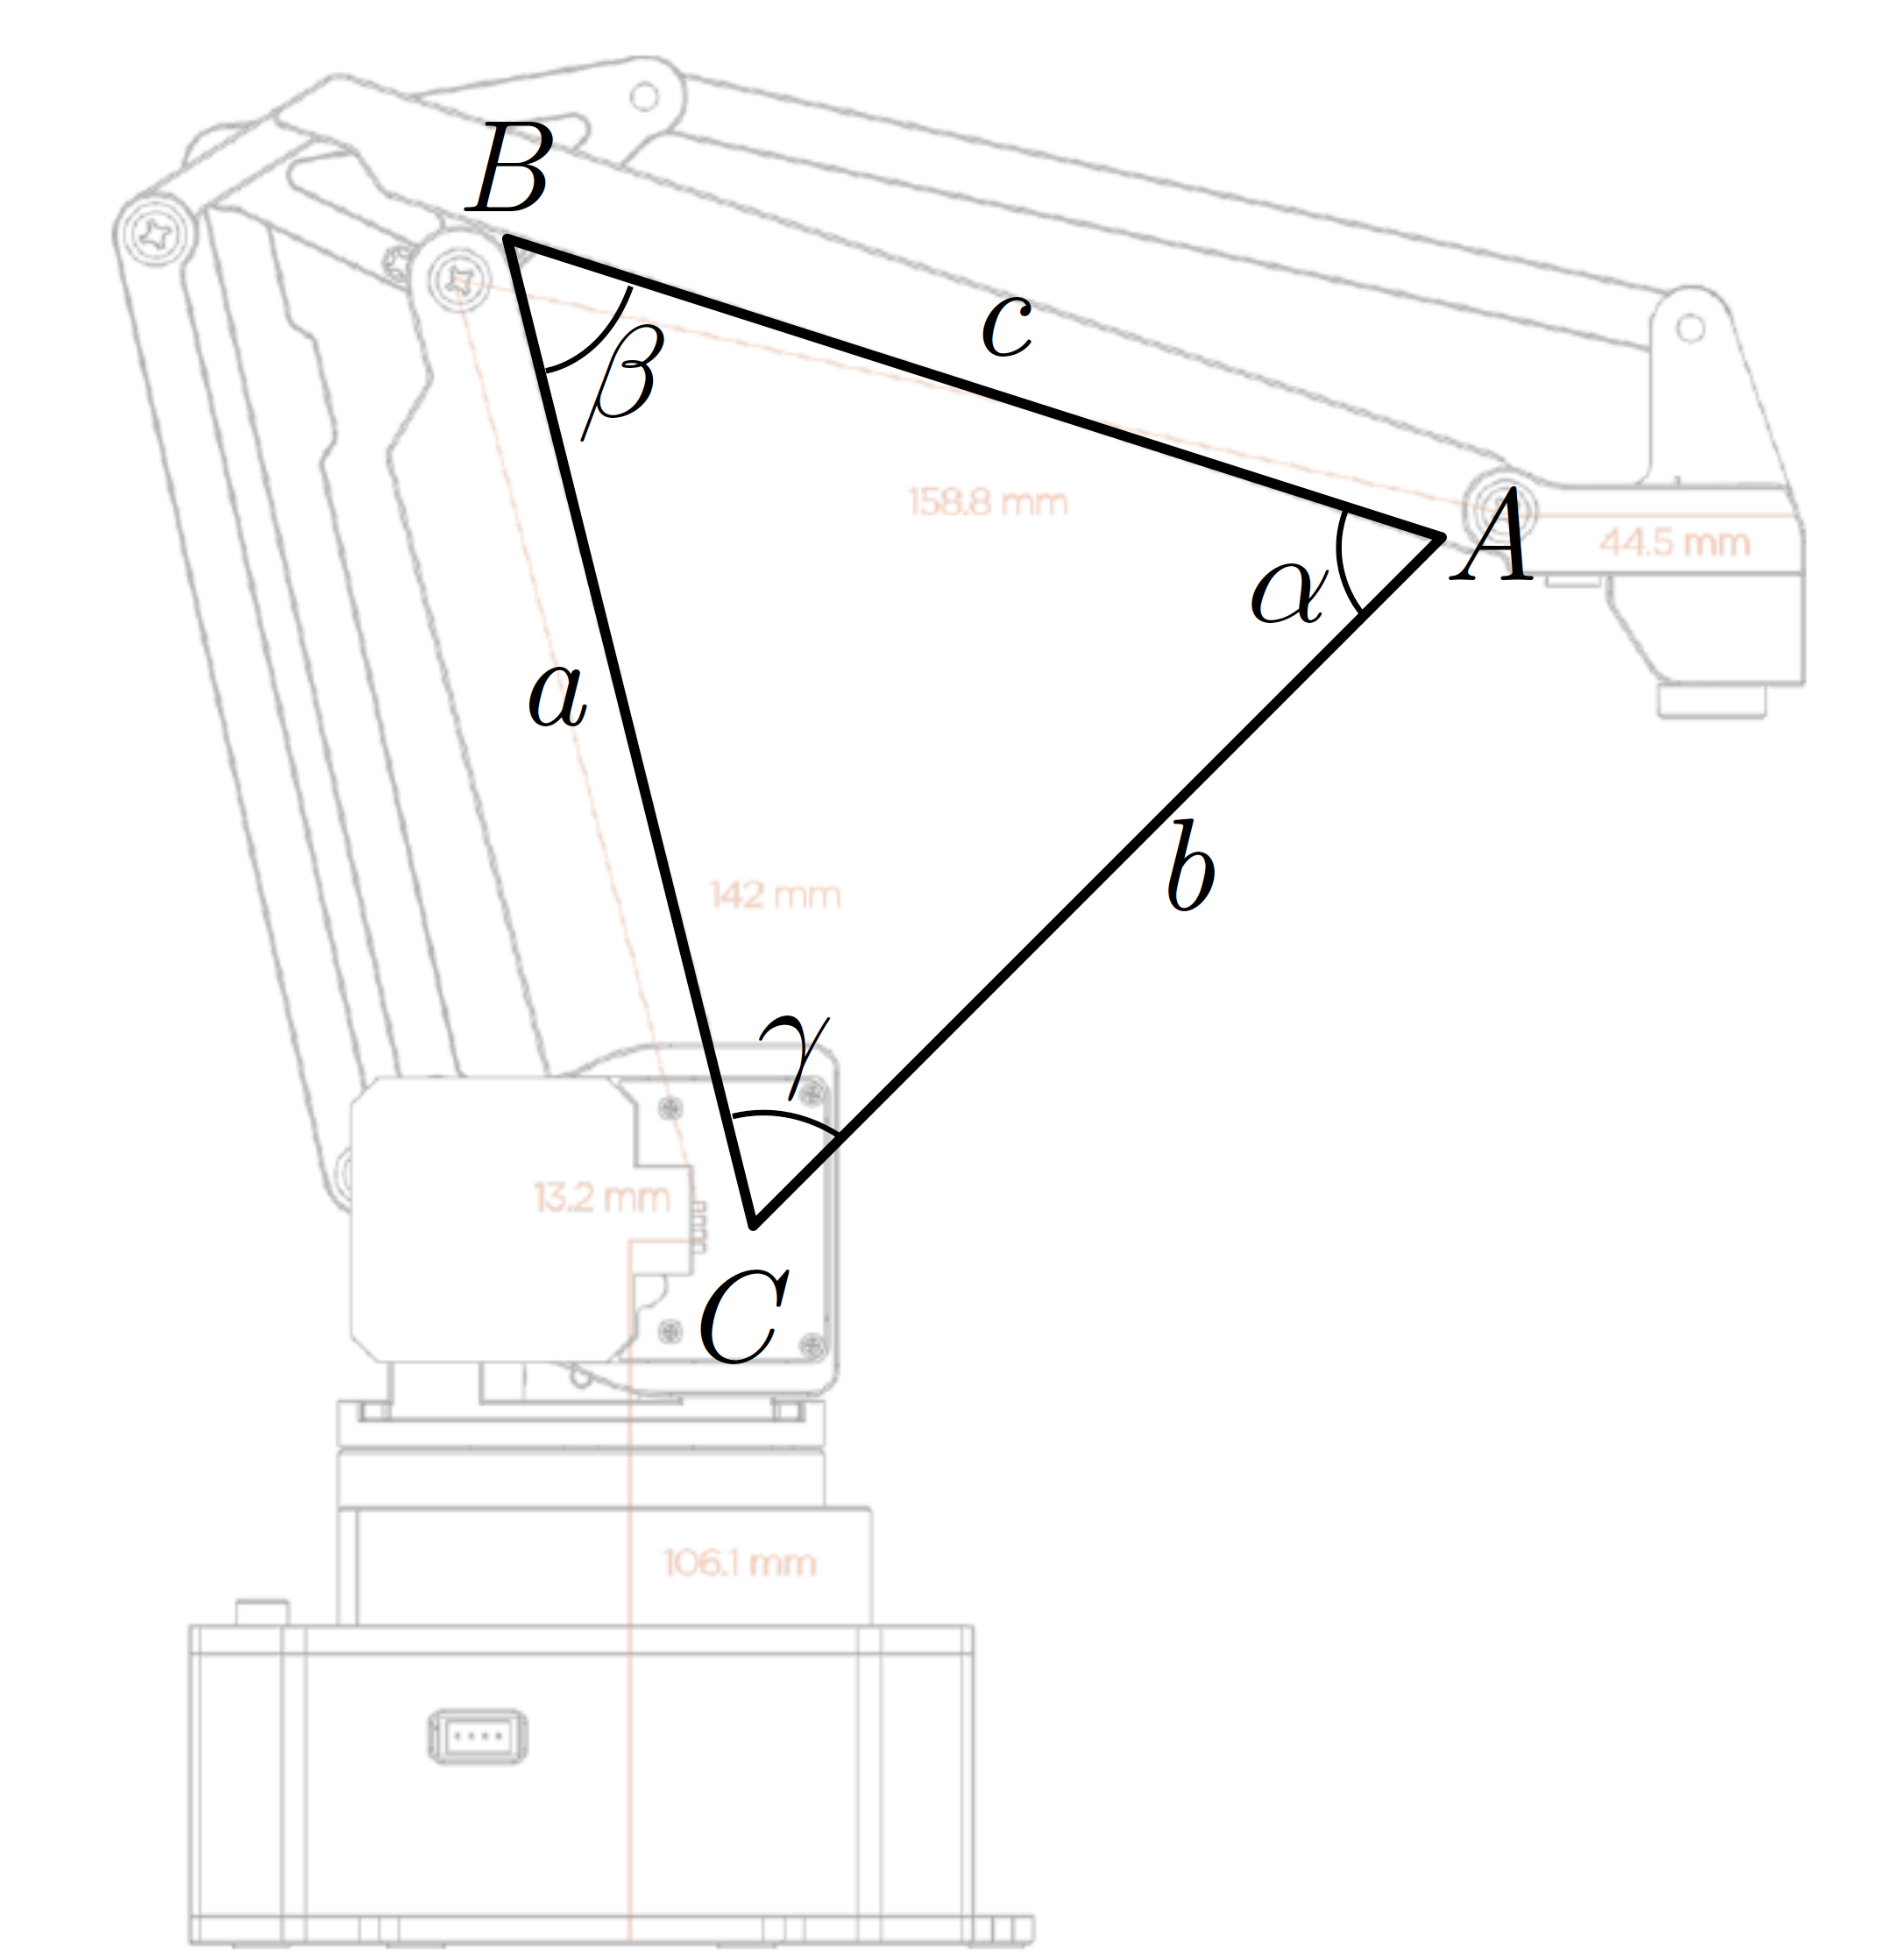
\includegraphics[width=.5\linewidth]{pictures/ik_cosine_law_over_arm.png}
    \caption{Parte superior del \pArm{} con el triángulo para obtener la cinemática inversa.}
    \label{fig:ik_over_arm}
\end{figure}

La distribución en particular del triángulo permite aplicar el teorema del coseno (ecuación
\ref{eq:cosine_law}) y obtener así los lados o bien los ángulos.

\begin{equation}\label{eq:cosine_law}
    c^2 = a^2 + b^2 - 2ab\cos{\gamma}
\end{equation}

En particular, para el brazo robótico se conocen siempre el tamaño de los lados
(según la figura \ref{fig:ik_over_arm}) `$a$' y `$c$', pero el lado `$b$' es variable. Según las
medidas del brazo se tiene que:

\begin{equation*}
    \left\{
    \begin{aligned}
        a & = \numprint[mm]{142}   \\
        c & = \numprint[mm]{158.8}
    \end{aligned}
    \right.
\end{equation*}

Como dicho lado `$b$' es desconocido en principio y además los ángulos $\left\{\gamma, \beta, \alpha\right\}$
también lo son, no se podría aplicar el teorema del coseno ya que se necesita cumplir alguna de las
siguientes condiciones:

\begin{itemize}
    \item Se conocen dos lados y el ángulo entre ellos.
    \item Se conocen los tres lados.
    \item Se conocen dos lados y el ángulo opuesto a ellos.
\end{itemize}

Dado que conocemos dos de los lados siempre y, según las características de un triángulo,
los ángulos no varían si y solo si la proporción de los lados es la misma tras aplicar
distintas operaciones que modifiquen su tamaño, se puede redimensionar el triángulo
mostrado en la figura \ref{fig:ik_over_arm} con la intención de buscar que el lado
desconocido sea unitario, esto es, mida $\numprint[mm]{1}$, pudiendo aplicar así en particular una forma del
teorema del coseno que permite obtener el ángulo `$\gamma$' teniendo los tres lados $\left\{a,b,c\right\}$
(ecuación \ref{eq:cosine_law_angle}):

\begin{equation}\label{eq:cosine_law_angle}
    \gamma = \arccos{\left(\frac{-a^2 - b^2 + c^2}{-2ab}\right)}
\end{equation}

\begin{figure}[H]
    \centering
    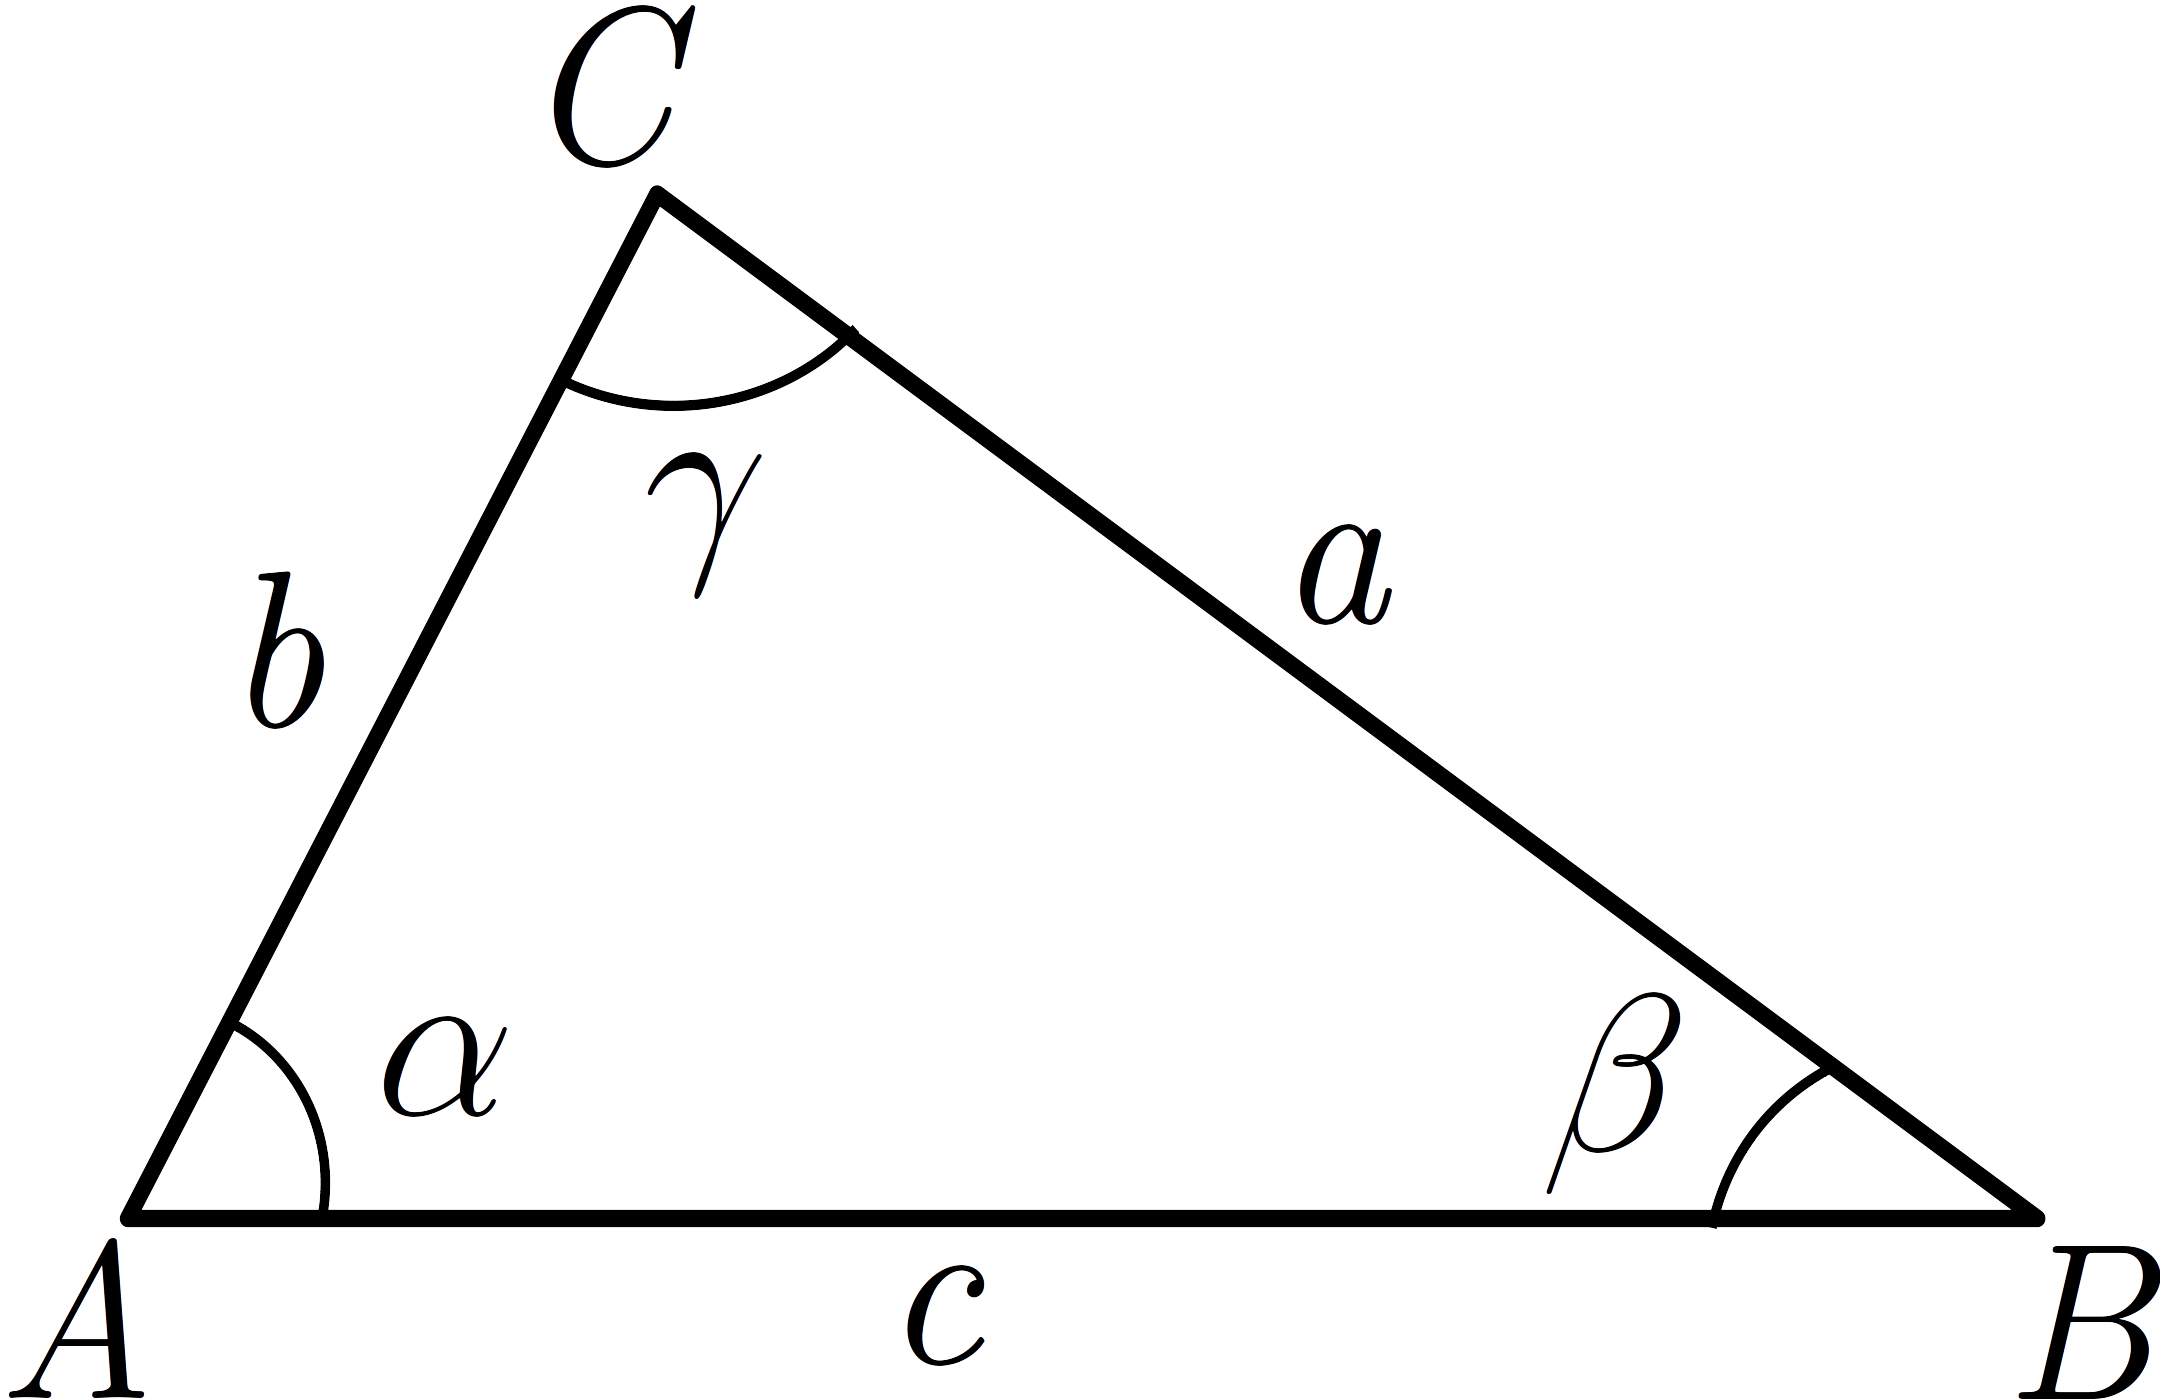
\includegraphics[width=.3\linewidth]{pictures/cosine_law.png}
    \caption{Triángulo para la aplicación del teorema del coseno en la ecuación \ref{eq:cosine_law_angle}.}
    \label{fig:cosine_law_triangle}
\end{figure}

Del triángulo mostrado en la figura \ref{fig:ik_over_arm} se conocen siempre las longitudes
`$a$' y `$c$'. La distancia `$b$' sin embargo también se puede obtener. Para la cinemática
inversa se tiene el punto $\left(x, y, z\right)$ que referencia la posición final del
\textit{end--effector}. En la figura \ref{fig:ik_over_arm}, el triángulo que se muestra
está situado sobre el plano $XYZ$ (ya que la rotación de la base es en el plano $XY$
y afecta a la posición final), por lo que de los puntos anteriores
se sabe que el \textit{end--effector} se sitúa en: $P_{ee} = \left(x', y, z'\right)$, 
por lo que se puede definir un vector desde la base $\overrightarrow{x'yz'}$ que 
represente el lado `$b$'. Como se puede apreciar, no se usan los puntos $\left(x, z\right)$ 
originales sino que previamente es necesario modificarlos:
\begin{itemize}
    \item Para la coordenada `$x$' se ha de reducir la longitud del \textit{end--effector}
    $\left(\overline{A_{EF_L}}\right)$ junto con la desviación de la base $\left(\overline{A_{B_D}}\right)$
    (ecuación \ref{eq:x_prime}):
    \begin{equation}\label{eq:x_prime}
        x' = x - \overline{A_{EF_L}} - \overline{A_{B_D}} = x - 44.5 - 13.2 = x - 57.7
    \end{equation}
    
    \item Para la coordenada `$z$' es necesario quitar la altura de la base $\left(A_{B_h}\right)$
    además de añadir la altura del \textit{end--effector} $h_o$ para dejar un punto 
    relativo al $\left(0\right)$. Así, el punto $z'$ se puede definir
    como (ecuación \ref{eq:z_prime}):
    \begin{equation}\label{eq:z_prime}
        z' = z - A_{B_h} + h_o = z - 106.1 + 16.01 = z - 90.09
    \end{equation}
\end{itemize}

Como el movimiento del brazo se realiza sobre un plano tridimensional, la posición y
longitud desde la base hasta $P_{ee}$ requiere tener en cuenta las tres coordenadas
$\left(x, y, z\right)$. Por ejemplo, la posición $y = \numprint[mm]{200}$ solo es 
alcanzable si el brazo está estirado al completo, pero en ese punto $x = 0$, al igual
que la posición $x = \numprint[mm]{200}$ solo es alcanzable si $y = 0$ (esto se muestra
en la figura \ref{fig:arm_limits}).

\begin{figure}[H]
    \begin{minipage}{.45\linewidth}
        \centering
        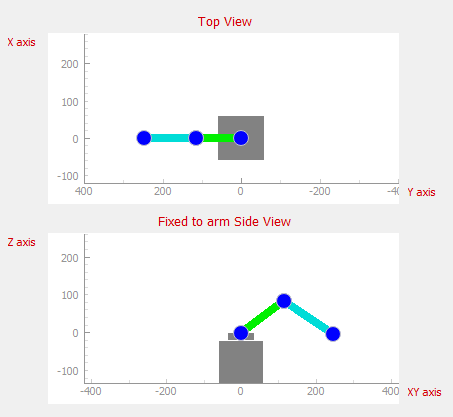
\includegraphics[width=\linewidth]{pictures/arm_y_max.png}
        \caption{Posición máxima en `$y$', donde $x = 0$.}
    \end{minipage}
    \hfill
    \begin{minipage}{.45\linewidth}
        \centering
        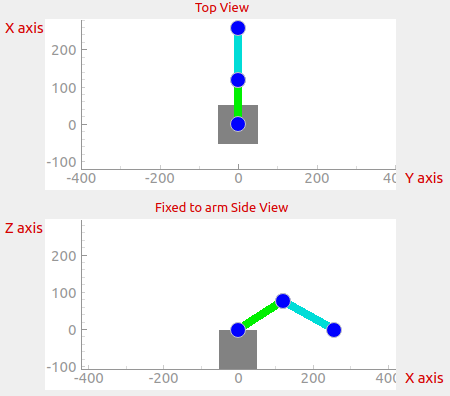
\includegraphics[width=\linewidth]{pictures/arm_x_max.png}
        \caption{Posición máxima en `$x$', donde $y = 0$.}
    \end{minipage}
    \caption{Demostración de la correlación entre `$x$' e `$y$'.}
    \label{fig:arm_limits}
\end{figure}

Con estos datos ya obtenidos se puede definir el lado `$b$' como:
\begin{equation*}
    b = \left|\overrightarrow{x'yz'}\right| = \sqrt{x'^2 + y^2 + z'^2}
\end{equation*}

Cabe destacar que $h_o$ varía según el \textit{end--effector} que se encuentre acoplado
al brazo robótico. Para el $\mu$Arm, según la documentación oficial, dichas alturas varían
y son\cite{UArmDeveloperSwiftProForArduino}:
\begin{itemize}
    \item $\numprint[mm]{74.55}$ para el \textit{end--effector} normal.
    \item $\numprint[mm]{51.04}$ para el cabezal láser.
    \item $\numprint[mm]{74.43}$ para el cabezal 3D.
    \item $\numprint[mm]{74.43}$ para el cabezal con bolígrafo.
    \item $\numprint[mm]{16.01}$ si no hay ningún \textit{end--effector} conectado.
\end{itemize}

Para el \pArm{}, en esta primera versión del desarrollo, se establece $h_o = \numprint[mm]{16.01}$.

Con las modificaciones en los lados ya listas, se puede definir un triángulo que cumple que:
\begin{itemize}
    \item Tiene dos lados fijos, `$a$' y `$c$', donde:
    \begin{equation*}
        \left\{\begin{aligned}
            a &= \overline{A_L} = \numprint[mm]{142.07} \\
            c &= \overline{A_U} = \numprint[mm]{158.8}
        \end{aligned}\right.
    \end{equation*}
    \item Tiene un lado variable `$b$' definido por el vector $\overrightarrow{x'z'}$
    y cuya longitud es: $b = \left|\overrightarrow{x'yz'}\right| = \sqrt{x'^2 + y^2 + z'^2}$.
\end{itemize}
Así, el triángulo resultante se define según las siguientes dimensiones y ángulos (figura
\ref{fig:ik_triangle}):

\begin{figure}[H]
    \centering
    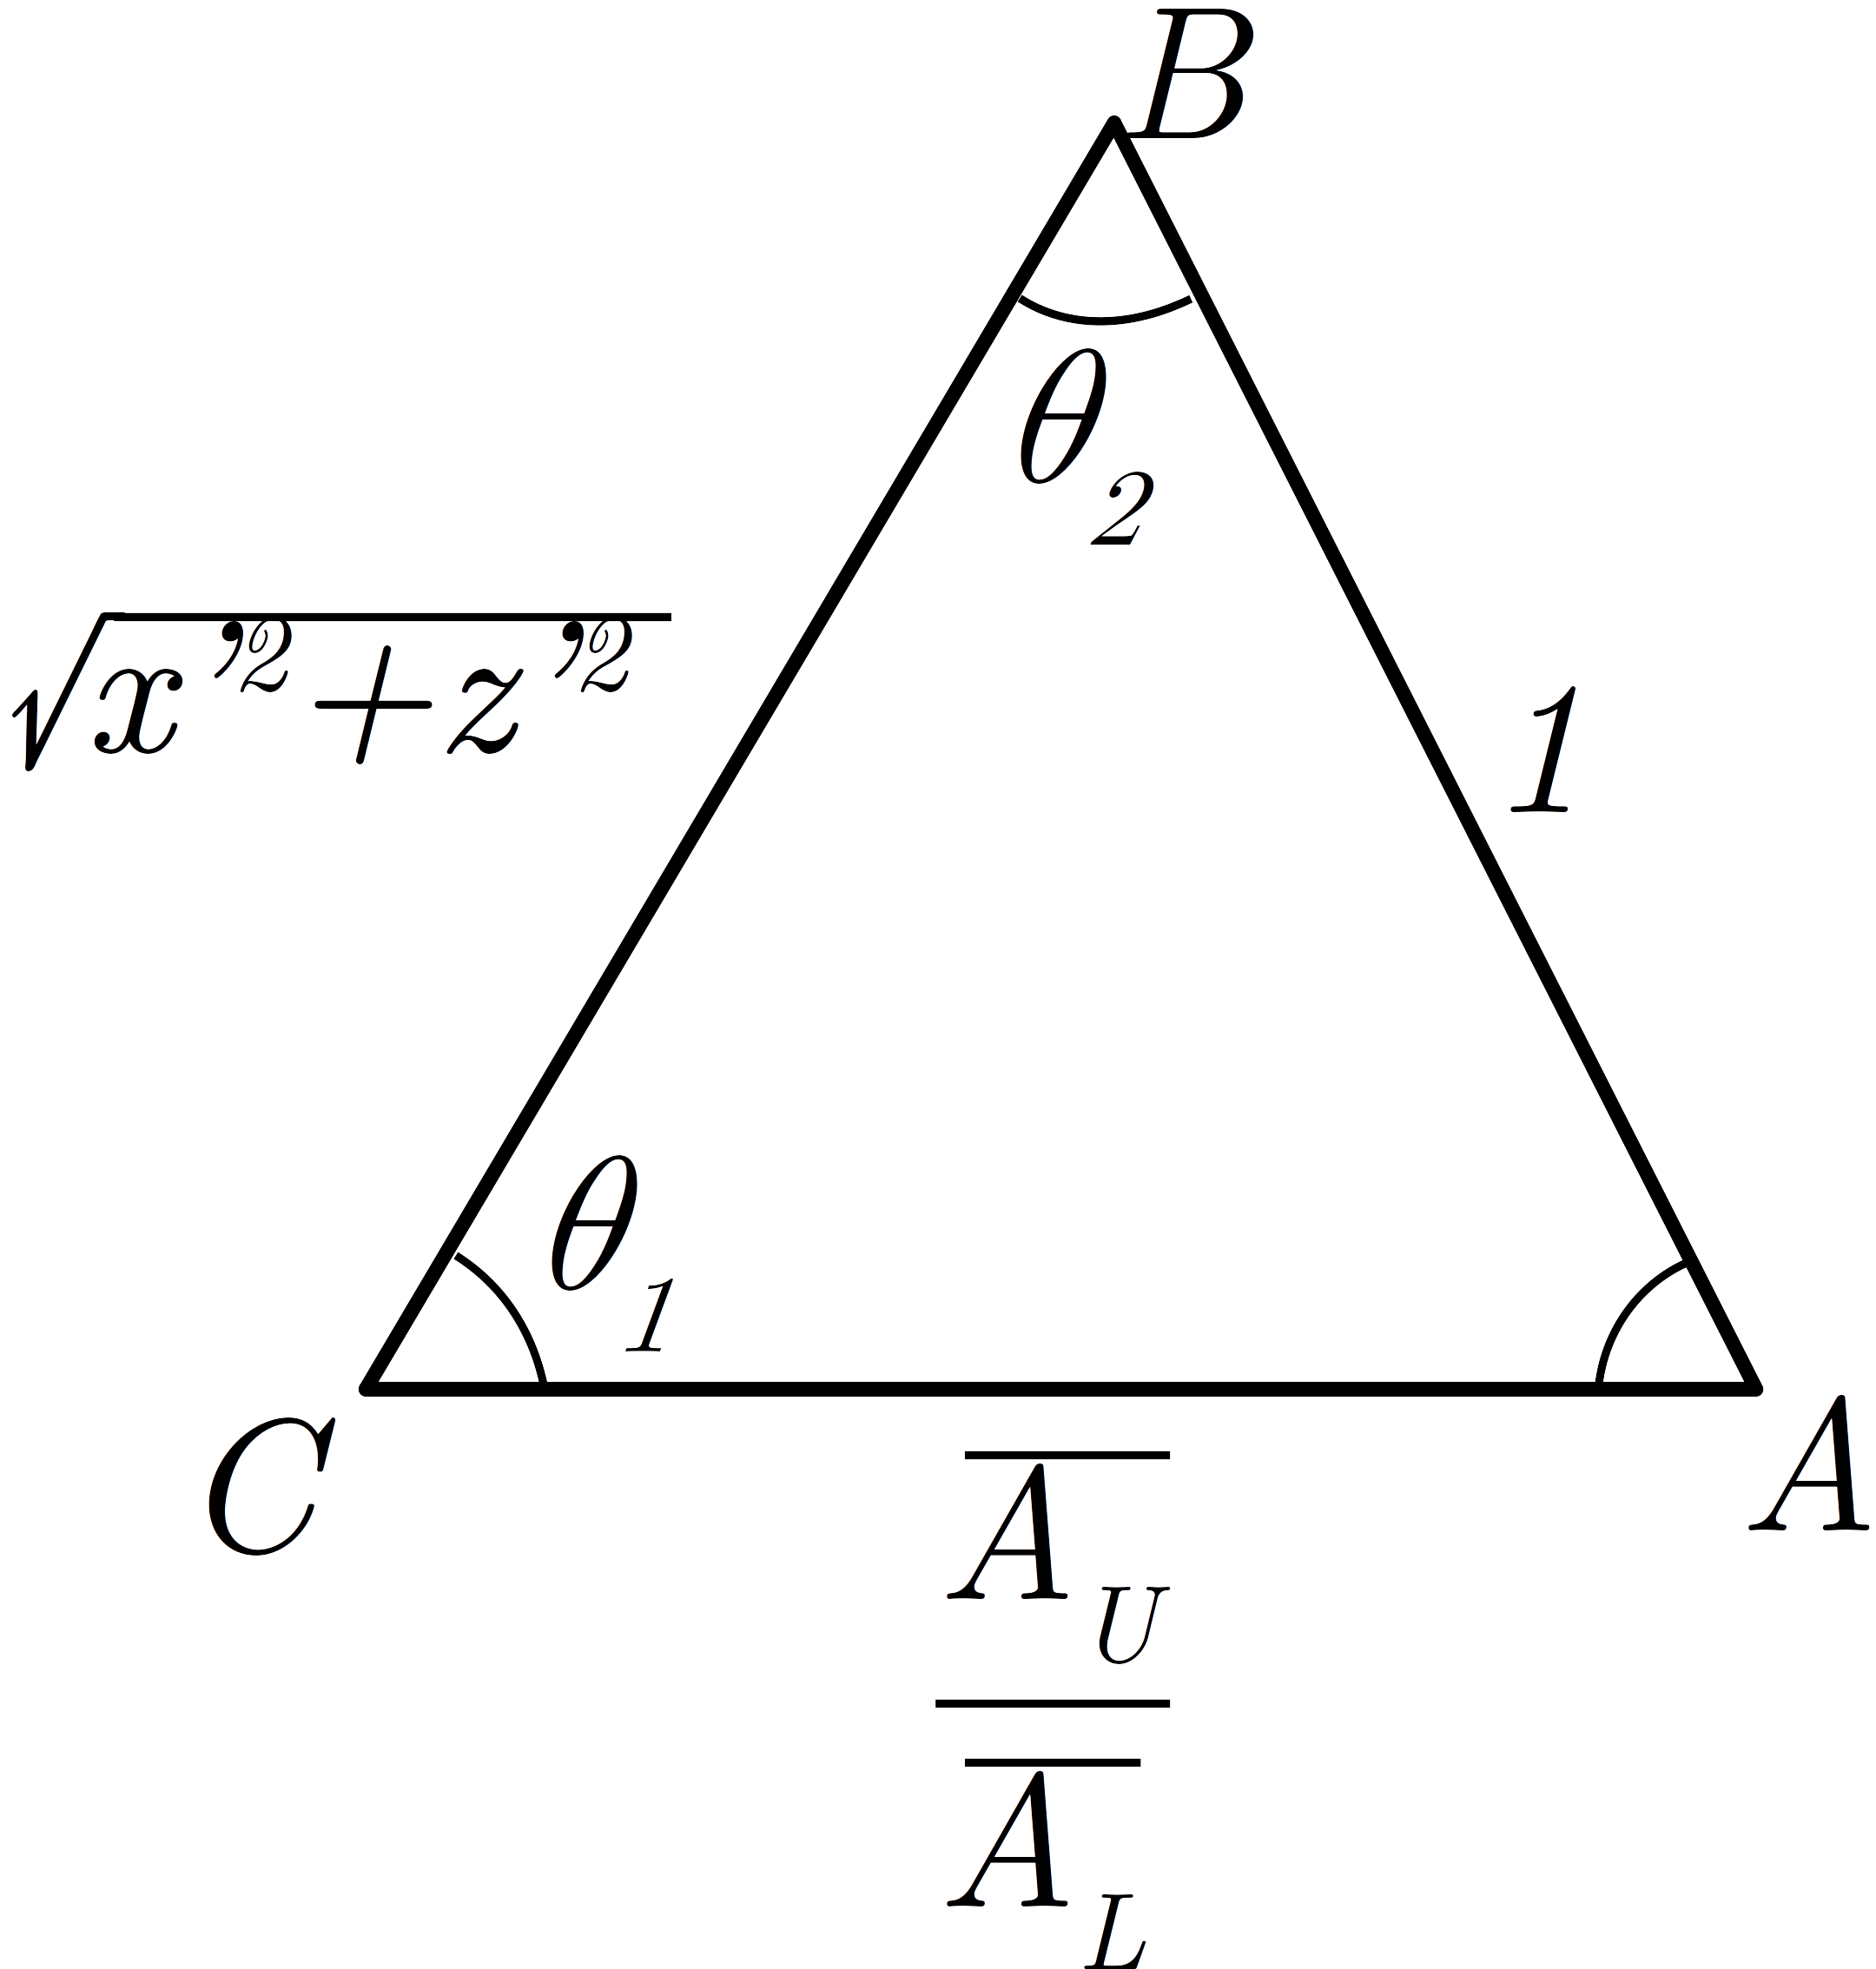
\includegraphics[width=.4\linewidth]{pictures/ik_unitary_triangle.png}
    \caption{Triángulo resultante tras aplicar las modificaciones a los lados.}
    \label{fig:ik_triangle}
\end{figure}

En particular, el triángulo anterior se puede colocar a modo de
referencia sobre el brazo tal como se muestra en la imagen \ref{fig:u_triangle_over_arm}:

\begin{figure}[H]
    \centering
    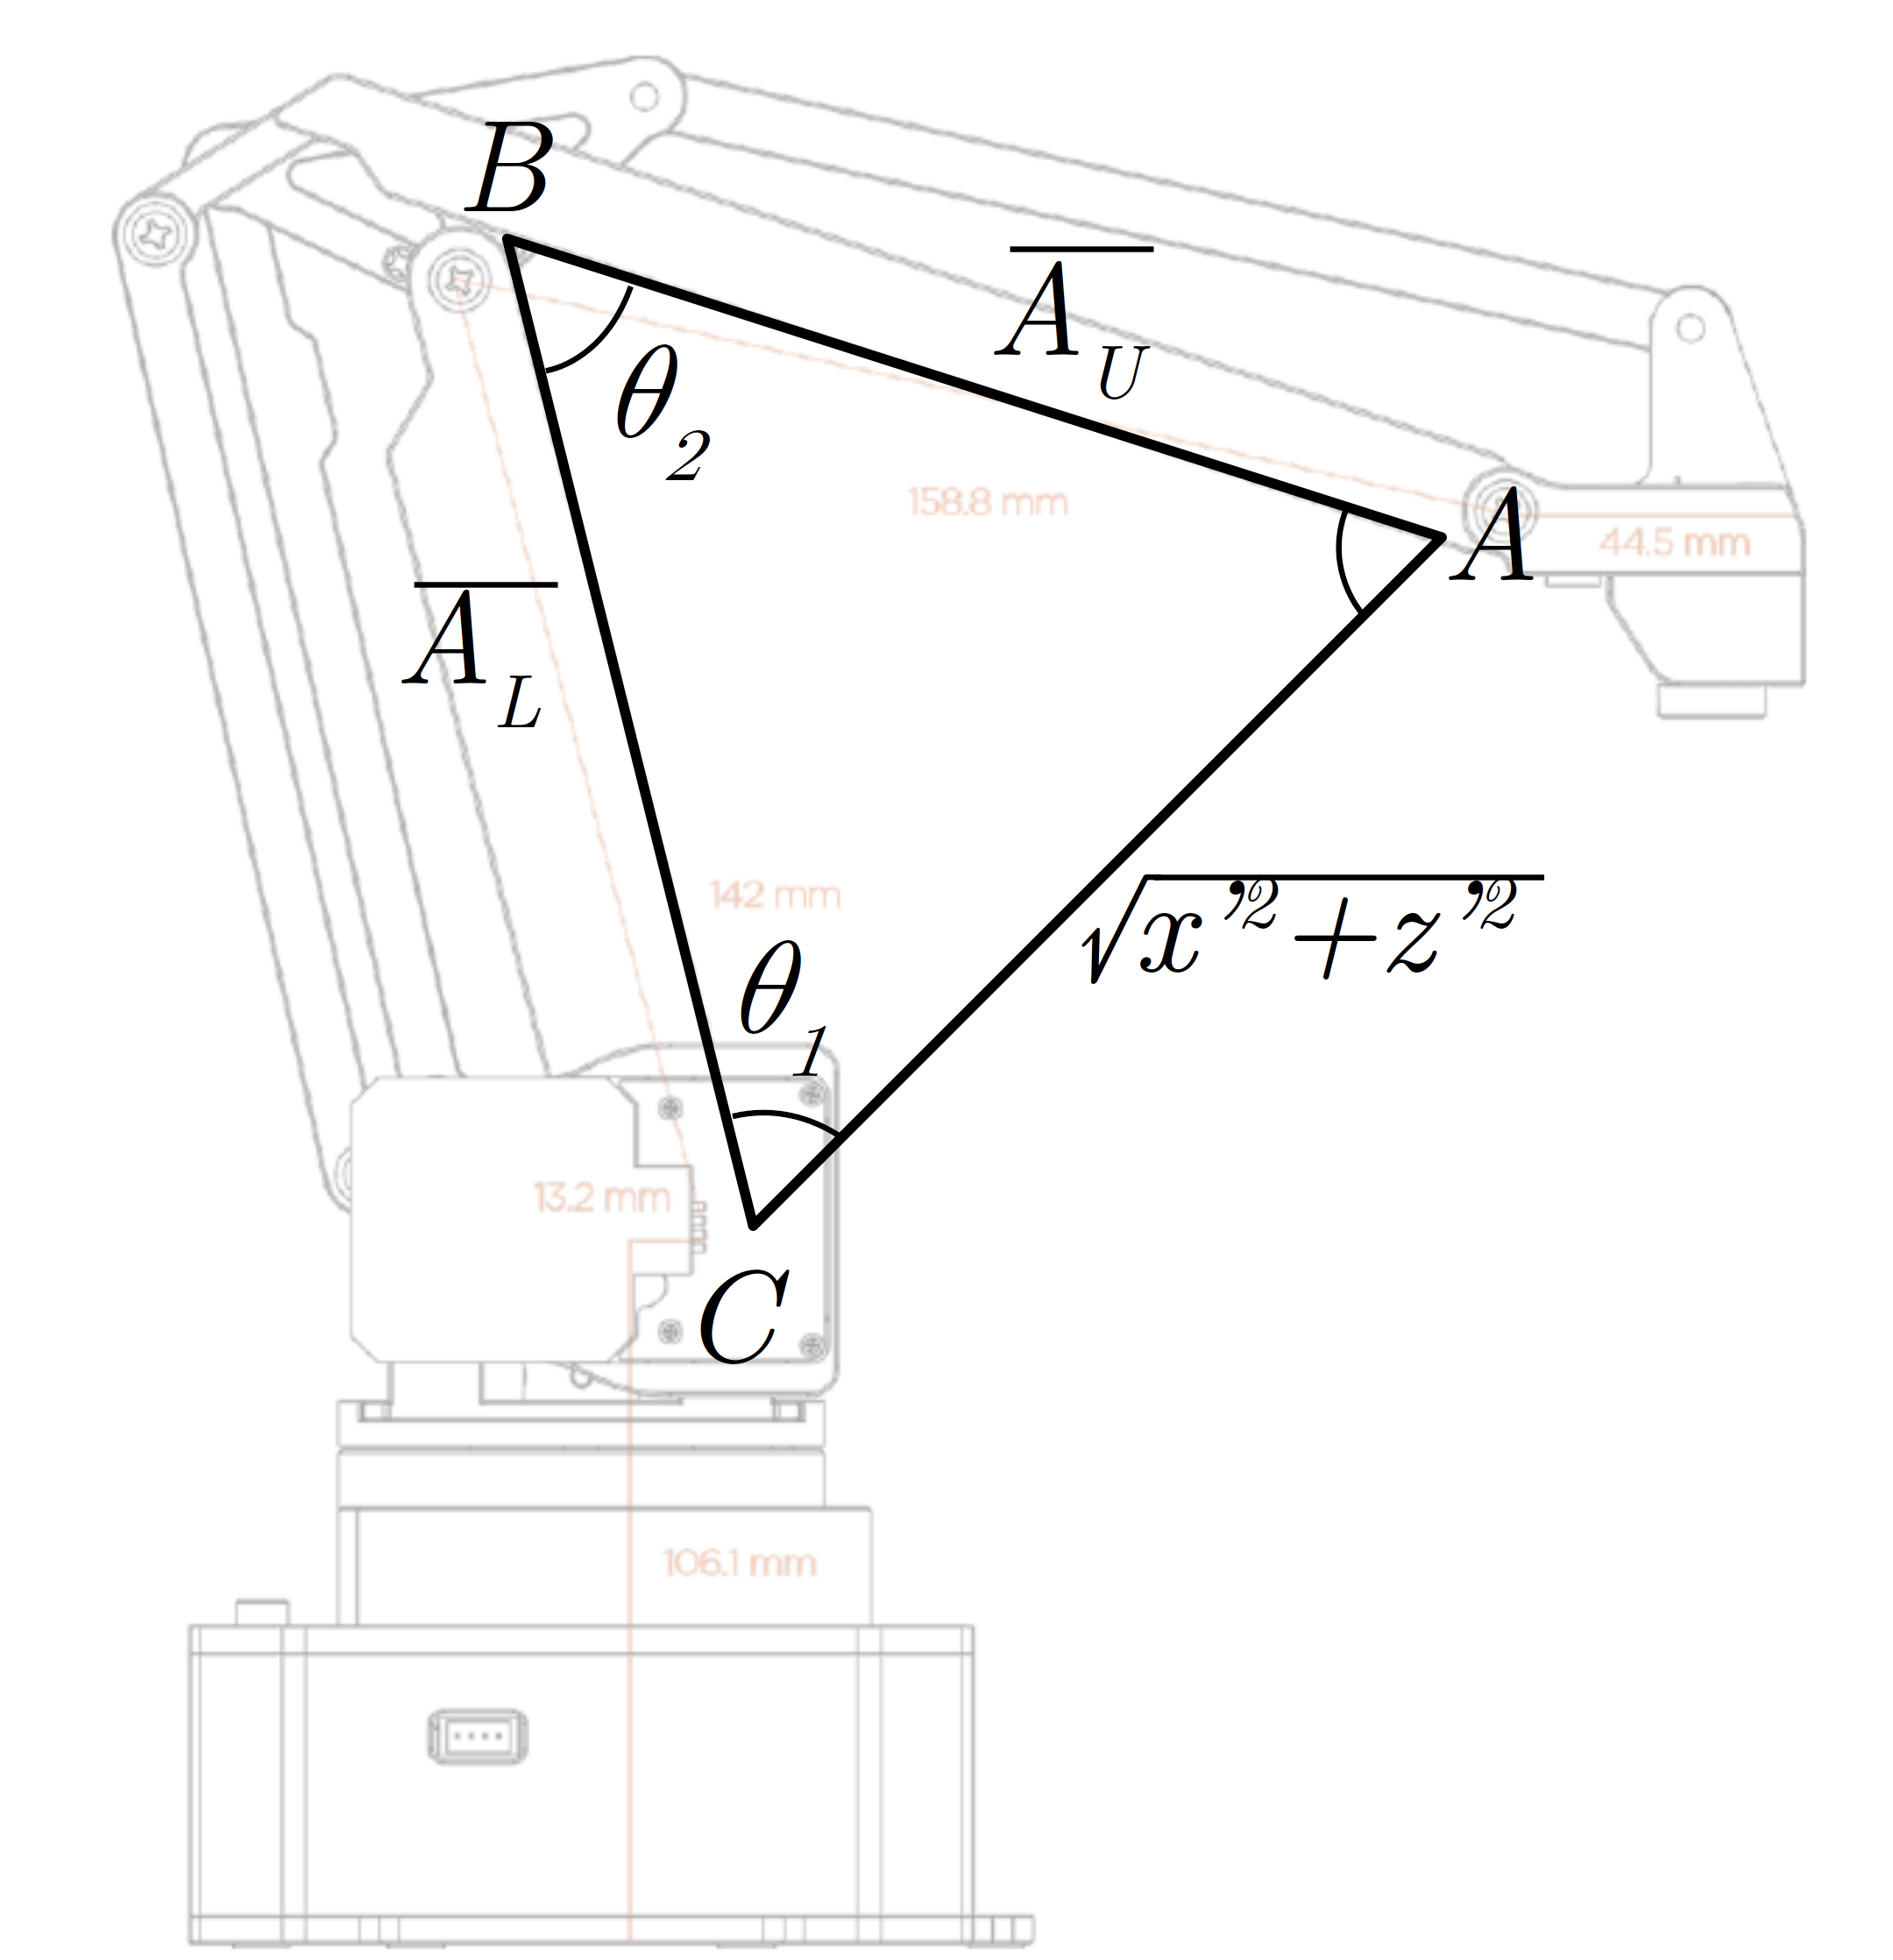
\includegraphics[width=.6\linewidth]{pictures/ik_triangle_over_arm.png}
    \caption{El triángulo colocado a modo de referencia sobre el \pArm{}.}
    \label{fig:u_triangle_over_arm}
\end{figure}

Para el triángulo mostrado en la figura \ref{fig:ik_triangle} se aplica
dos veces el teorema del coseno (ecuación \ref{eq:cosine_law_angle}) para obtener
los valores de $\theta_1'$ (ver ecuación \ref{eq:t1}) y $\theta_2'$ (ver ecuación \ref{eq:t2}):

\begin{align}
    \theta_1' & = \arccos{\left(\frac{-\overline{A_L}^2 - \left(x'^2 + y^2 + z'^2\right) + \overline{A_U}^2} %
    {-2 \overline{A_L} \sqrt{x'^2 + y^2 + z'^2}}\right)} \label{eq:t1} \\[2ex]
    \theta_2 & = \arccos{\left(\frac{-\overline{A_L}^2 - \overline{A_U}^2 + x'^2 + y^2 + z'^2} %
    {-2 \overline{A_L} \cdot \overline{A_U}}\right)} \label{eq:t2}
\end{align}

Como se puede apreciar en las ecuaciones anteriores, todavía no se tienen los valores finales
de los ángulos sino una primera aproximación a ellos. Esto es debido a que el ángulo
$\theta_1$ que aparece en el triángulo de la figura \ref{fig:ik_triangle}
no se encuentra paralelo al plano del suelo, en este caso, el plano $XY$ (tal y como se puede ver
en la figura \ref{fig:u_triangle_over_arm}).

Para poder obtener los ángulos reales se ha de añadir el ángulo `$\phi$' que relaciona el triángulo
\ref{fig:u_triangle_over_arm} con el plano del suelo, tal y como se puede ver en la figura
\ref{fig:final_triangle}:

\begin{figure}[H]
    \centering
    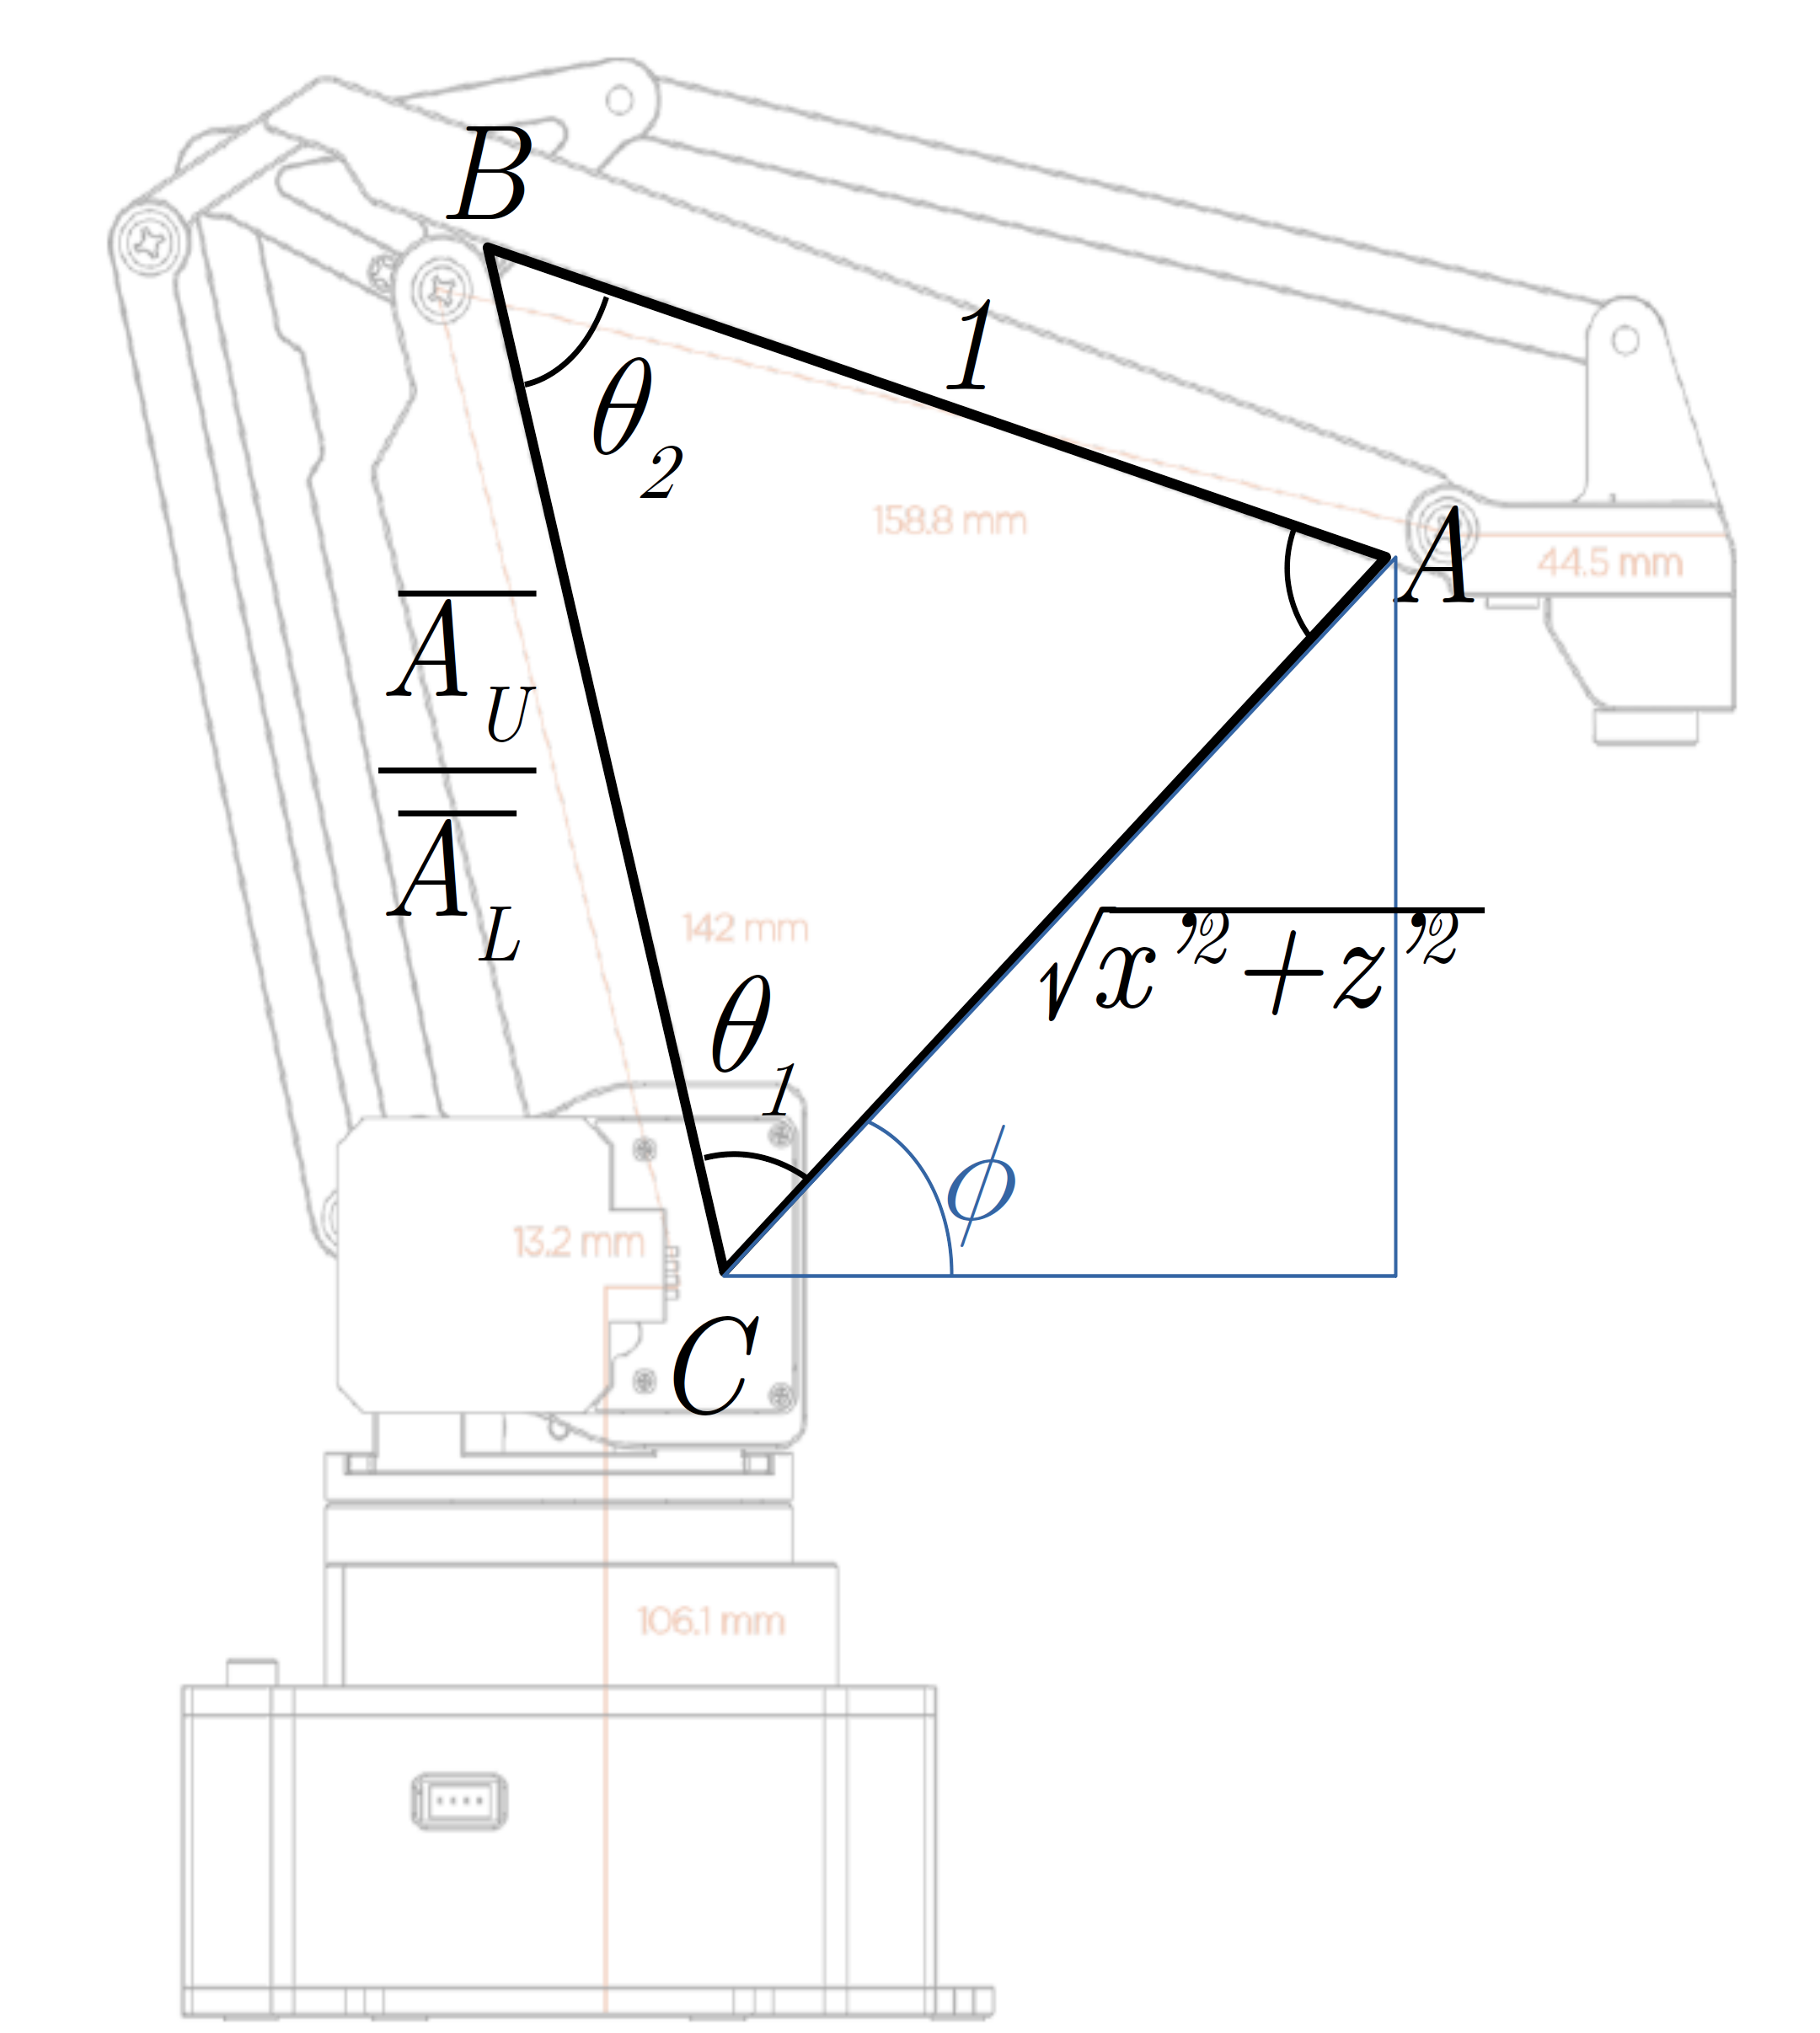
\includegraphics[width=.5\linewidth]{pictures/ik_final.png}
    \caption{Triángulo final orientativo junto con el ángulo $\phi$ respecto al plano del suelo.}
    \label{fig:final_triangle}
\end{figure}

La obtención de dicho ángulo se muestra en la ecuación \ref{eq:phi}

\begin{equation}\label{eq:phi}
    \phi = \arctan{\frac{z'}{\sqrt{x'^2 + y^2}}}~rad
\end{equation}

y $\theta_1$ se obtiene mediante la ecuación
\ref{eq:final_theta}\footnote{el ángulo $\phi$ se suma o se resta según la orientación
    del triángulo ya que la arcotangente varía en signo según la posición de los puntos
    $x'$ y $z'$, tal como se muestra en la documentación al desarrollador\cite{UArmDeveloperSwiftProForArduino}.}:

\begin{equation}\label{eq:final_theta}
    \theta_1 = \theta_1' - \phi
\end{equation}

Finalmente, por seguridad, se puede comprobar que en efecto los distintos ángulos obtenidos
están comprendidos dentro del rango de movimiento de cada una de las articulaciones
\cite{UArmDeveloperSwiftProForArduino}:

\begin{align*}
    \theta_0 & \in \left[\frac{\pi}{18}, \frac{151}{180}\pi\right] \\
    \theta_1 & \in \left[0, \frac{113}{150}\pi\right]              \\
    \theta_2 & \in \left[0, \frac{1199}{1800}\pi\right]
\end{align*}
\section{Funciones jacobianas}
Previo a comenzar este apartado, se quiere destacar que dicho apartado ha sido
introducido con la única intención de plantear un análisis estrictamente cinemático
(no dinámico) del movimiento del robot.

Las matrices Jacobianas son una herramienta que permite definir la relación
dinámica entre dos representaciones diferentes de un sistema. Para un manipulador
de $n$ grados de libertad (con $n > 1$) se puede definir la posición del mismo de dos
formas posibles:

\begin{enumerate}
    \item Mediante la posición y orientación del \textit{end--effector}, denominado por $x$.
    \item Mediante el conjunto de los ángulos de las articulaciones, denominado por $q$.
\end{enumerate}

El modo de funcionamiento de las matrices Jacobianas se puede definir como el efecto
que se produce en el \textit{end--effector} `$x$' tras un movimiento de las articulaciones
`$q$', entendiendo así la Jacobiana como la matriz transformada de la velocidad.

Formalmente, la matriz Jacobiana se define como un conjunto de ecuaciones diferenciales
parciales (denotado en la ecuación \ref{eq:jacobian_def}):

\begin{equation}\label{eq:jacobian_def}
    J = \frac{\partial x}{\partial q}
\end{equation}

la cual puede ser expresada como:

\begin{equation}\label{eq:jacobian_x}
    \dot{x} = J \cdot \dot{q}
\end{equation}

donde $\dot{x}$ y $\dot{q}$ representan las derivadas de $x, q$ respecto al tiempo.

En la ecuación \ref{eq:jacobian_x} se expresa que la velocidad del \textit{end--effector}
es igual al producto de la Jacobiana $J$ multiplicada por la velocidad de las articulaciones.
¿Para qué resulta útil tener estos datos? La expresión \ref{eq:jacobian_x} permite el
trabajar con trayectorias en un espacio diferente al que se dispone normalmente\cite{travisdewolfRobotControlPart2013a}.
Esto permite el control del \textit{end--effector} mediante la
generación de señales de control (en términos de fuerza) a aplicar en $\left(x, y, z\right)$.
Las matrices Jacobianas pues permiten un cálculo directo de las señales de control en un
espacio controlado, como son los torques de los motores/articulaciones, dada otra señal
que no controlamos, como la fuerza a aplicar en el \textit{end--effector}.

Anteriormente se ha visto que la Jacobiana representa la relación entre velocidades
parciales del \textit{end--effector} y las articulaciones, pero se ha hablado de trabajar
con las fuerzas de cada uno de ellos. Para el \pArm{}, se pueden definir las siguientes
premisas:

\begin{align*}
    x & = \left[x, y, z\right]^T                      \\
    q & = \left[\theta_0, \theta_1, \theta_2\right]^T
\end{align*}

Como se conoce la velocidad, se puede definir el trabajo $\left(W\right)$ como la fuerza
que hay que aplicar durante una distancia, definido por la ecuación \ref{eq:work}. Por
otra parte, la potencia $\left(P\right)$ se define como la cantidad de trabajo efectuado
por unidad de tiempo\cite{PotenciaFisica2020}, definido por la ecuación \ref{eq:power}.

\begin{align}
    W & = \int{F^T \cdot v~dt} \label{eq:work}   \\[1ex]
    P & = \frac{W}{\varDelta t} \label{eq:power}
\end{align}

Atendiendo a lo comentado anteriormente, se puede afirmar que es equivalente
representar el movimiento del brazo articulado en base al movimiento de sus
articulaciones a representarlo en base a la velocidad del \textit{end--effector}.

\subsection*{Construyendo la matriz Jacobiana}
Como se mostró anteriormente, la velocidad del \textit{end--effector} se puede
expresar como el producto de la matriz Jacobiana por la velocidad de las articulaciones
(ecuación \ref{eq:jacobian_x}). Para dicha ecuación se tienen los siguientes datos:

\begin{equation*}
    \dot{x} = J \cdot \dot{q}
    \left\{\begin{aligned}
        \dot{x} & = \left(X_e, Y_e, Z_e, \phi_e\right)                        \\
        \dot{q} & = \left(\theta_0, \cdots, \theta_n,~d_1, \cdots, d_n\right) \\
        J       & = \text{matriz Jacobiana}
    \end{aligned}\right.
\end{equation*}

La obtención de la matriz Jacobiana $J\left(\dot{q}\right)$ se ha de realizar obteniendo
las submatrices Jacobianas que relacionan la velocidad lineal `$v$' y la velocidad angular
`$\omega$'. La matriz Jacobiana que relaciona la velocidad lineal se define como
(ecuación \ref{eq:j_v}):

\begin{equation}\label{eq:j_v}
    J_v\left(\dot{q}\right) =
    \begin{bmatrix}
        \frac{\partial X_e}{\partial \theta_0} & \frac{\partial X_e}{\partial \theta_1} & \cdots & \frac{\partial X_e}{\partial \theta_n} & \frac{\partial X_e}{\partial d_1} & \cdots & \frac{\partial X_e}{\partial d_n} \\[3ex]
        \frac{\partial Y_e}{\partial \theta_0} & \frac{\partial Y_e}{\partial \theta_1} & \cdots & \frac{\partial Y_e}{\partial \theta_n} & \frac{\partial Y_e}{\partial d_1} & \cdots & \frac{\partial Y_e}{\partial d_n} \\[3ex]
        \frac{\partial Z_e}{\partial \theta_0} & \frac{\partial Z_e}{\partial \theta_1} & \cdots & \frac{\partial Z_e}{\partial \theta_n} & \frac{\partial Z_e}{\partial d_1} & \cdots & \frac{\partial Z_e}{\partial d_n} \\
    \end{bmatrix}
\end{equation}

y la matriz que relaciona la velocidad angular se define como (ecuación \ref{eq:j_w}):

\begin{equation}\label{eq:j_w}
    J_{\omega}\left(\dot{q}\right) =
    \begin{bmatrix}
        \frac{\partial \phi_X}{\partial \theta_0} & \frac{\partial \phi_X}{\partial \theta_1} & \cdots & \frac{\partial \phi_X}{\partial \theta_n} & \frac{\partial \phi_X}{\partial d_1} & \cdots & \frac{\partial \phi_X}{\partial d_n} \\[3ex]
        \frac{\partial \phi_Y}{\partial \theta_0} & \frac{\partial \phi_Y}{\partial \theta_1} & \cdots & \frac{\partial \phi_Y}{\partial \theta_n} & \frac{\partial \phi_Y}{\partial d_1} & \cdots & \frac{\partial \phi_Y}{\partial d_n} \\[3ex]
        \frac{\partial \phi_Z}{\partial \theta_0} & \frac{\partial \phi_Z}{\partial \theta_1} & \cdots & \frac{\partial \phi_Z}{\partial \theta_n} & \frac{\partial \phi_Z}{\partial d_1} & \cdots & \frac{\partial \phi_Z}{\partial d_n} \\
    \end{bmatrix}
\end{equation}

De esta manera, la matriz Jacobiana `$J$' se puede definir como
(ecuación \ref{eq:j})\footnote{el cálculo de las matrices Jacobianas puede resultar
    complejo de realizar sobre todo a nivel simbólico, por lo que se deja en el anexo
    \ref{anex:jupyter_binder} un enlace a un \textit{Jupyter Notebook} que agiliza y guía
    durante el proceso de obtención de estas matrices. El código fuente para su obtención
    no obstante se encuentra disponible en el anexo \ref{lst:manipulator_py}.}:

\begin{gather}\label{eq:j}
    J_{ee}\left(\dot{q}\right) =
    \begin{bmatrix}
        J_v\left(\dot{q}\right) \\[1ex]
        J_{\omega}\left(\dot{q}\right)
    \end{bmatrix} = \\[2ex]
    {\footnotesize
    \begin{bmatrix}
     - \left(a_{1} + a_{2} \cos{\theta_{1}} + a_{3} \cos{\theta_{1} - \theta_{2}}\right) \sin{\theta_{0}} &  \left(- a_{2} \sin{\theta_{1}} - a_{3} \sin{\theta_{1} - \theta_{2}}\right) \cos{\theta_{0}} &  a_{3} \sin{\theta_{1} - \theta_{2}} \cos{\theta_{0}} \\
     \left(a_{1} + a_{2} \cos{\theta_{1}} + a_{3} \cos{\theta_{1} - \theta_{2}}\right) \cos{\theta_{0}} &  \left(- a_{2} \sin{\theta_{1}} - a_{3} \sin{\theta_{1} - \theta_{2}}\right) \sin{\theta_{0}} &  a_{3} \sin{\theta_{0}} \sin{\theta_{1} - \theta_{2}} \\
     0 &  a_{2} \cos{\theta_{1}} + a_{3} \cos{\theta_{1} - \theta_{2}} &  - a_{3} \cos{\theta_{1} - \theta_{2}} \\[2ex]
     0 &  1 &  -1 \\
     0 &  0 &  0 \\
     1 &  0 &  0 \\
    \end{bmatrix}} \nonumber
\end{gather}

Una de las utilidades de la matriz Jacobiana es la obtención de los puntos críticos,
es decir, aquellos en los que el determinante de dicha matriz se hace cero. Los puntos
críticos resultan de especial interés ya que definen posiciones en el manipulador que o
bien son inalcanzables o bien someten a la estructura física del mismo a una gran tensión,
pudiendo resultar dañado en el proceso o de llegar a una ``posición de no retorno'', donde
los motores que componen el brazo puede que no dispongan de suficiente fuerza para moverse a otra
posición.

Para la matriz Jacobiana anterior (ecuación \ref{eq:j}), se obtiene el siguiente
determinante (ecuación \ref{eq:j_det}):

\begin{equation}\label{eq:j_det}
    \left|J_{ee}\left(\dot{q}\right)\right| = - a_{2} a_{3} \left(a_{1} + a_{2} \cos{\theta_{1}} + a_{3} \cos{\theta_{1} - \theta_{2}}\right) \sin{\theta_{2}}
\end{equation}

Analíticamente se puede observar que los puntos críticos del \pArm{} se dan para
los valores de $\theta_2 = 0$ y $\theta_2 = \pi$, punto en el que el brazo está o bien
completamente recogido o bien completamente estirado. La cuestión radica en que, viendo
la configuración geométrica del brazo robótico, el ángulo de $\pi~rad$ se
vuelve inalcanzable ya que los valores máximos del ángulo $\theta_2$ son \cite{ufactoryUArmDeveloperSwiftProForArduino}:

\begin{equation*}
    \theta_2 \in \left[0, \frac{1199}{1800}\pi\right]
\end{equation*}

Por el contrario, la posición de $0~rad$ se habrá de tener en cuenta para
evitar que el brazo esté expuesto a un nivel elevado de tensión durante tiempo prolongado.
Entre los dos segmentos superiores del brazo robótico se situará un fin de carrera a
efectos de evitar dicha tensión además de regular y calibrar los motores.

Al igual que en el caso de la cinemática directa, se puede obtener una matriz Jacobiana
inversa que permite, dada la velocidad lineal del \textit{end--effector} $\dot{x}$, obtener qué par han
de generar las articulaciones $\dot{q}$ para obtener dicha fuerza. La Jacobiana inversa
depende directamente de que el determinante sea distinto de cero ya que, en otro caso,
implicará que la matriz es una matriz singular y que por consiguiente no es invertible
\cite{InvertibleMatrix2020}.

Para el caso anterior existe una ``pseudo--inversa'' de Moore--Penrose \cite{PseudoinversaMoorePenrose2020}
la cual permite la obtención de una matriz inversa aún cuando su determinante es cero.
Dicha pseudo--inversa se denota $J^+$ y se define por (ecuación \ref{eq:j+}):

\begin{equation}\label{eq:j+}
    J^+ = J^T (J \cdot J^T)^{-1}
\end{equation}

Además, se cumple que si la inversa de la matriz Jacobiana existe entonces su pseudo--inversa
también existirá, y será igual a la matriz inversa:

\begin{equation*}
    J^+ = J^{-1} \iff \exists J^{-1}
\end{equation*}

Como los puntos críticos son $\theta_2 = 0$ y $\theta_2 = \pi$ se puede obtener un valor
de la inversa que será igual a la pseudo--inversa, donde ambas dependen del parámetro
$\theta_2$ para existir. El valor que se obtiene de la inversa es el siguiente (ecuación
\ref{eq:pinv})\footnote{el cálculo simbólico de tanto la inversa como de la pseudo--inversa
    puede resultar algo complejo por lo que se ha dejado en el anexo \ref{anex:jupyter_binder}
    un \textit{Jupyter Notebook} para realizar las operaciones de forma interactiva y guiada.
    No obstante, el código fuente se encuentra disponible en el anexo \ref{lst:manipulator_py}.}:

\begin{gather}\label{eq:pinv}
    J^{-1} = J^+ = \\
    {\footnotesize\begin{bmatrix}
        - \frac{\sin{\theta_{0}}}{a_{2} \cos{\theta_{1}} + a_{3} \cos{\theta_{1} - \theta_{2}} + a_{1}}                                   & \frac{\cos{\theta_{0}}}{a_{2} \cos{\theta_{1}} + a_{3} \cos{\theta_{1} - \theta_{2}} + a_{1}}                                     & 0                                                                                                   \\[3ex]
        - \frac{\cos{\theta_{0}} \cos{\theta_{1} - \theta_{2}}}{a_{2} \sin{\theta_{2}}}                                                   & - \frac{\sin{\theta_{0}} \cos{\theta_{1} - \theta_{2}}}{a_{2} \sin{\theta_{2}}}                                                   & - \frac{\sin{\theta_{1} - \theta_{2}}}{a_{2} \sin{\theta_{2}}}                                      \\[3ex]
        - \frac{\left(a_{2} \cos{\theta_{1}} + a_{3} \cos{\theta_{1} - \theta_{2}}\right) \cos{\theta_{0}}}{a_{2} a_{3} \sin{\theta_{2}}} & - \frac{\left(a_{2} \cos{\theta_{1}} + a_{3} \cos{\theta_{1} - \theta_{2}}\right) \sin{\theta_{0}}}{a_{2} a_{3} \sin{\theta_{2}}} & - \frac{a_{2} \sin{\theta_{1}} + a_{3} \sin{\theta_{1} - \theta_{2}}}{a_{2} a_{3} \sin{\theta_{2}}} \\[2ex]
    \end{bmatrix}} \nonumber
\end{gather}

No ha sido necesario emplear la matriz pseudo-inversa en este proyecto, pero se muestra
en el anexo \ref{anex:pinv} por si en un futuro interesa recurrir a ella.
Esta matriz ha sido calculada empleando un \textit{Jupyter Notebook} que se encuentra
en el anexo \ref{anex:jupyter_binder}.
\section{Implementación final realizada}
Una vez concluido el estudio sobre el fundamento matemático del proyecto, se decidió
qué usar de lo visto anteriormente.

Por una parte, se vio cómo el uso de la fuerza bruta generando un mapa de ángulos
y puntos resultaba inviable teniendo en cuenta el espacio disponible en el microcontrolador
así como el tiempo necesario para calcularlo.

Con respecto a las funciones Jacobianas, si bien su estudio permite crear muchas
relaciones entre velocidades y fuerzas, dado que la masa del robot es pequeña y la
velocidad es constante, el uso de dichas funciones para el control del mismo no añade
mucha más información de la que ya se dispone. Además, en favor de lo anterior, en el
código fuente original del $\mu$Arm tampoco contempla las funciones Jacobianas a la hora
de manejar ni los puntos ni la velocidad \cite{UArmDeveloperSwiftProForArduino}, por lo
que se puede asumir que su uso no es necesario.

Por esto mismo, el control del brazo se realizará utilizando la cinemática directa
para obtener el punto $\left\{x, y, z\right\}$ del \textit{end--effector} cuando se
aplican unos ángulos de entrada $\left\{\theta_0, \theta_1, \theta_2\right\}$; y la
cinemática inversa para obtener la relación entre un punto de entrada $\left\{x, y, z\right\}$
y los ángulos que lo generan $\left\{\theta_0, \theta_1, \theta_2\right\}$.

Teniendo en cuenta las características mencionadas sobre el microcontrolador a utilizar,
el tiempo de ambas operaciones es bastante pequeño (unos $\numprint[\mu s]{15}$ la
cinemática directa y $\numprint[\mu s]{100}$ para la cinemática inversa, según una
estimación con el simulador.), por lo que su uso no añade un desfase suficientemente
grande como para considerarse notorio.

\chapter{\textit{Hardware}}
\label{chap:hardware}
Los elementos \textit{hardware} conforman la implementación física del manipulador y de todos los componentes empleados para controlarlo.

En términos generales, el \textit{hardware} usado en el proyecto se descompone en diferentes elementos:
\begin{itemize}
    \item Impresión 3D de la estructura física del manipulador.
    \item Motores empleados en el manipulador.
    \item Desarrollo de la placa de circuito impreso de control y microcontrolador empleado.
    \item Comunicaciones entre los diferentes subsistemas.
\end{itemize}

En primer lugar, la impresión 3D es la tecnología seleccionada para la fabricación de la estructura física del manipulador debido a su bajo coste y accesibilidad. Esta parte del proyecto se centra en llevar a cabo la fabricación y construcción de la estructura física del manipulador, así como su ensamblado y testeo. Este apartado se ubica en el apartado 5.1 de la memoria.

En segundo lugar, la elección de los motores que dotan de movilidad a la estructura es una decisión crucial y que depende principalmente de cuales sean las características físicas del manipulador, así como de las tareas que se quieran realizar con el mismo. Existen numerosas opciones en cuanto a motores, por ejemplo, motores DC, servomotores, motores paso a paso, etc. Este apartado se ubica en el apartado \ref{sec:motors} de la memoria.

En tercer lugar, el desarrollo de la PCB de control y elección del microcontrolador representan la parte más importante dentro del bloque hardware del proyecto. El objetivo principal de esta parte del proyecto es llevar a cabo el diseño y construcción de una PCB personalizada, adaptada especialmente a los actuadores y microcontrolador usados para llevar a cabo el control del movimiento del manipulador. Se considera que esta PCB representa uno de los elementos hardware esenciales para el correcto desarrollo del proyecto. Este apartado se ubica en el apartado 5.3 de la memoria.

En último lugar, el diseño e implementación de los canales de comunicación y protocolos necesarios para comunicar los dos subsistemas principales requiere desarrollo hardware y software de forma equitativa, además, también representa uno de los elementos cruciales del proyecto. Este apartado se ubica en el apartado 5.4 de la memoria.





%% REVISADO
\section{Diseño 3D}
Las razones por las cuales se toma la decisión de fabricar la estructura del brazo mediante impresión 3D se detallan a continuación:

\begin{itemize}
  \item Cumplir con el objetivo de replicabilidad y asequibilidad: una de las bases del proyecto es que pueda ser reproducible a bajo coste tanto de recursos como de tiempo. Se decide por tanto construir la estructura física del brazo mediante técnicas de impresión 3D, ya que están altamente extendidas y son cada vez mas asequibles.
  
  \item Características físicas del material: los plásticos utilizado en impresión 3D suelen ser ligeros y suficientemente resistente para soportar las cargas para las que está pensado el manipulador.
  
  \item Disponibilidad de impresora 3D: dado que la Universidad es capaz de proveer al equipo con una impresora 3D, los costes del proyecto se abaratan si la estructura es realizada con los medios de los que la ya se disponen.
  
  \item Simplificar el proceso de mejora y personalización: debido a la naturaleza \ac{OS} y \ac{OH} del proyecto, se espera que las personas interesadas puedan contribuir a él, mejorándolo y/o personalizándolo. Además, la impresión 3D facilita estas acciones.
\end{itemize}

En particular, la impresora que la Universidad pone a disposición del equipo de trabajo es la ``\textit{Ultimaker 3 Extended}'', la cual es capaz de imprimir en una alta variedad de materiales, de los cuales destacan los siguientes:

\begin{itemize}
    \item \ac{PLA}\cite{AcidoPolilactico2020}: este material permite imprimir de manera segura con alta precisión dimensional y una resistencia a la tracción excepcional, que además soporta grandes velocidades de impresión y es biodegradable, ya que se obtienen a partir de almidón de maíz, de yuca, mandioca o de caña de azúcar. 
    \item \ac{ABS}\cite{AcrilonitriloButadienoEstireno2020}: material que presenta buena adhesión entre capas y una resistencia a temperaturas de hasta 85ºC. Permite obtener buenos detalles estéticos.
    \item Ultimaker Nylon: este material es un tipo de poliamida basada en los polímeros plásticos PA6/66. Presenta una absorción de humedad reducida así como una capacidad considerable de resistencia ante tensiones mecánicas junto con un bajo coeficiente de fricción, haciéndolo un material ideal para construcciones mecánicas.
    \item CPE y CPE+: este material presenta una alta estabilidad dimensional, con buena resistencia al impacto y a la temperatura. Debido a su alta solidez y su estabilidad dimensional ofrece un buen rendimiento mecánico y gran resistencia al desgaste.
\end{itemize}

Debido a la naturaleza mecánica del proyecto, el equipo ha decidido emplear materiales con alta resistencia mecánica para las piezas móviles. El Ultimaker Nylon junto con el CPE cumplen con dicha característica.

Por otro lado, los componentes que no sean móviles como carcasas o  
piezas protectoras se imprimirán en PLA ya que tras realizar pruebas, el equipo de desarrollo ha concluido que el material es lo suficientemente resistente para soportar los pesos a los que será sometido.

Aprovechando la licencia original GPL 3.0 del $\mu$Arm, se ha recuperado el modelo 3D proporcionado por UFACTORY como punto de partida. 
Dicho modelo se ha tomado como punto de partida para el \pArm{}, teniendo que realizar diversas
modificaciones de distintas piezas para adaptarlas a los materiales que se van a usar,
los motores que se emplearán y el tamaño de la nueva placa, entre otros.

\begin{figure}[H]
    \centering
    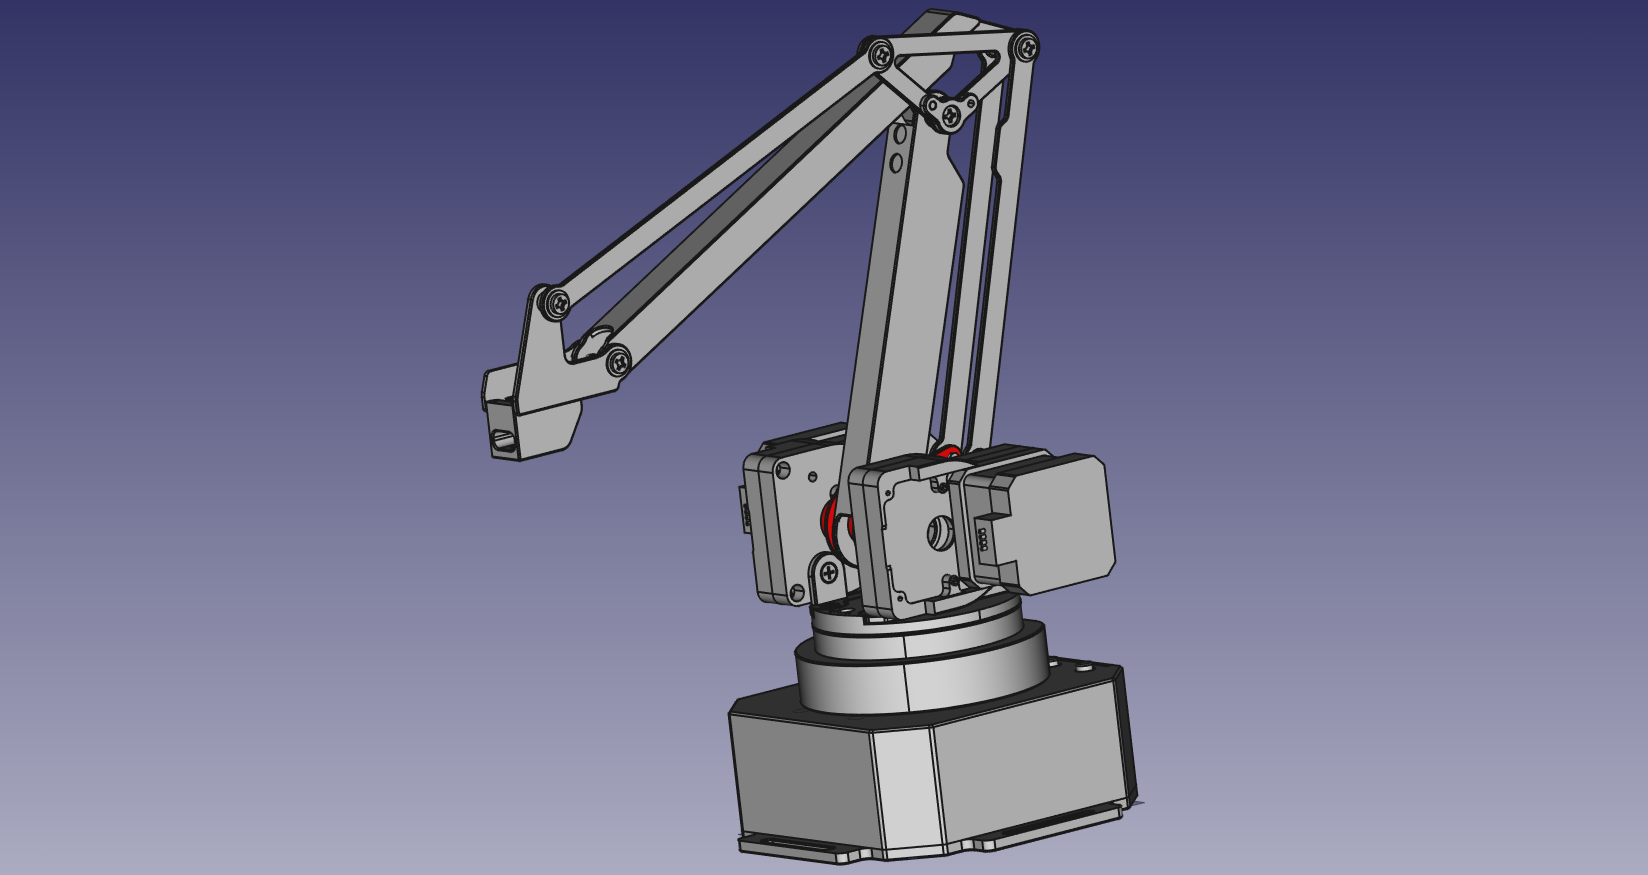
\includegraphics[width=.8\linewidth]{pictures/brazo_vista_3d_inicial.png}
    \caption{Concepto inicial del brazo robótico.}
    \label{fig:manipulador_inicial}
\end{figure}

Las herramientas que han sido empleadas para visualizar y modificar el modelo y posteriormente imprimir las piezas han sido respectivamente FreeCAD y Ultimake Cura.

\begin{figure}[H]
    \centering
    
\includegraphics[width=.45\linewidth]{pictures/freeCAD.jpg}
    \hspace{1cm}
    
\includegraphics[width=.40\linewidth]{pictures/Ultimaker_cura_logo.png}
    \caption{Logotipos de las herramientas utilizadas.}
    \label{fig:herramientas_3d}
\end{figure}

El flujo de trabajo que se ha seguido desde el modelo 3D hasta la impresión de una pieza ha sido el mostrado en la figura \ref{fig:flujo_3d}:

\begin{figure}[H]
    \centering
    \includegraphics[width=.9\linewidth]{pictures/DiagramaImpresión.jpg}
    \caption{Flujo de trabajo del desarrollo y la impresión 3D.}
    \label{fig:flujo_3d}
\end{figure}

Antes de proceder a explicar cada una de las nuevas piezas que se han diseñado, se tomará una de ellas como ejemplo para explicar el proceso de diseño detallado.

Inicialmente se parte de un bloque que represente la forma general de la pieza, para posteriormente añadir detalles. En el caso de la pieza que se usa como ejemplo, tenemos un cuadrado de 120mm de ancho por 120mm de alto y 3 mm de groso.

\begin{figure}[H]
\centering
\subfigure[Plano vacío]{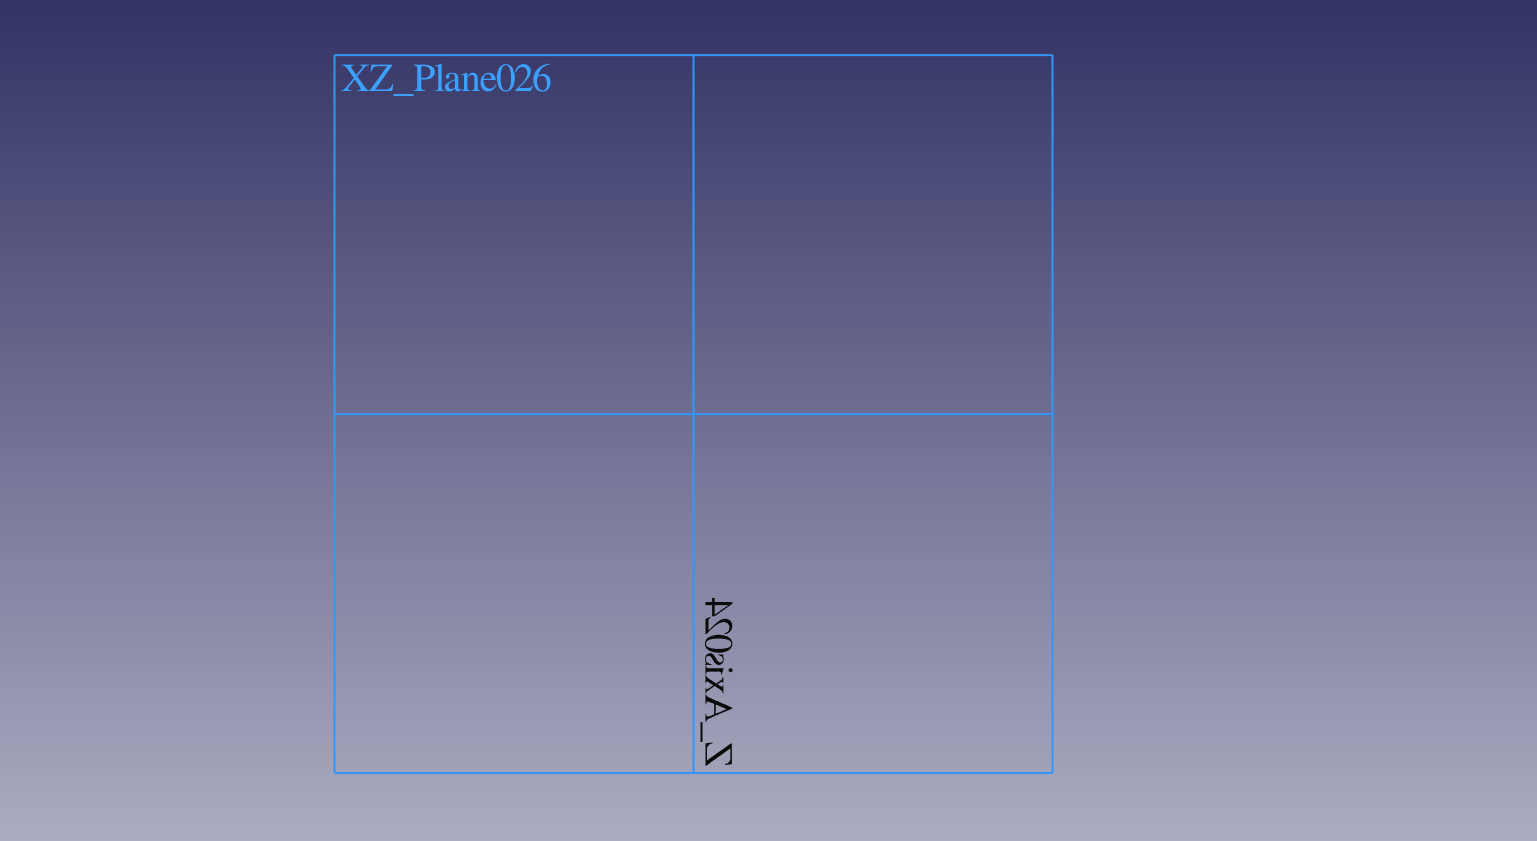
\includegraphics[width=82mm]{pictures/PlanoVacio.png}}
\subfigure[Forma general de la tapa]{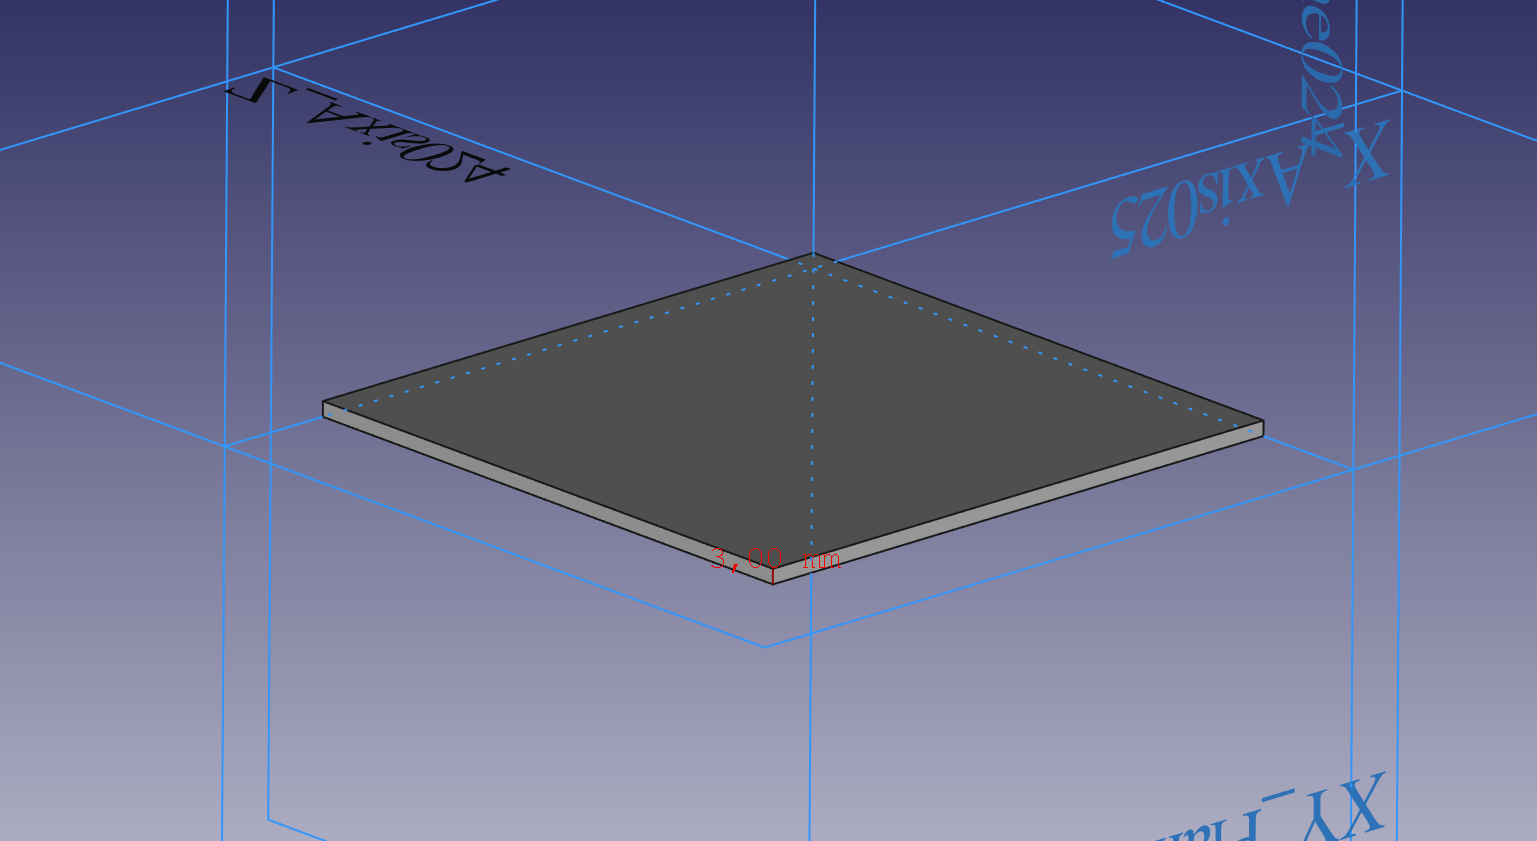
\includegraphics[width=82mm]{pictures/SketchTapaInicial.png}}
\caption{Construcción de la forma general}
\label{fig:forma_general_tapa_superior}
\end{figure}

Tras crear la forma general, añadimos los agujeros en las esquinas para poder atornillar la tapa. Los agujeros tienen un radio de 1,9mm y se distancian de los laterales 3,9mm para hacerlos coincidir con los agujeros de las paredes.

\begin{figure}[H]
\centering
\subfigure[Plano 2D de los agujeros]{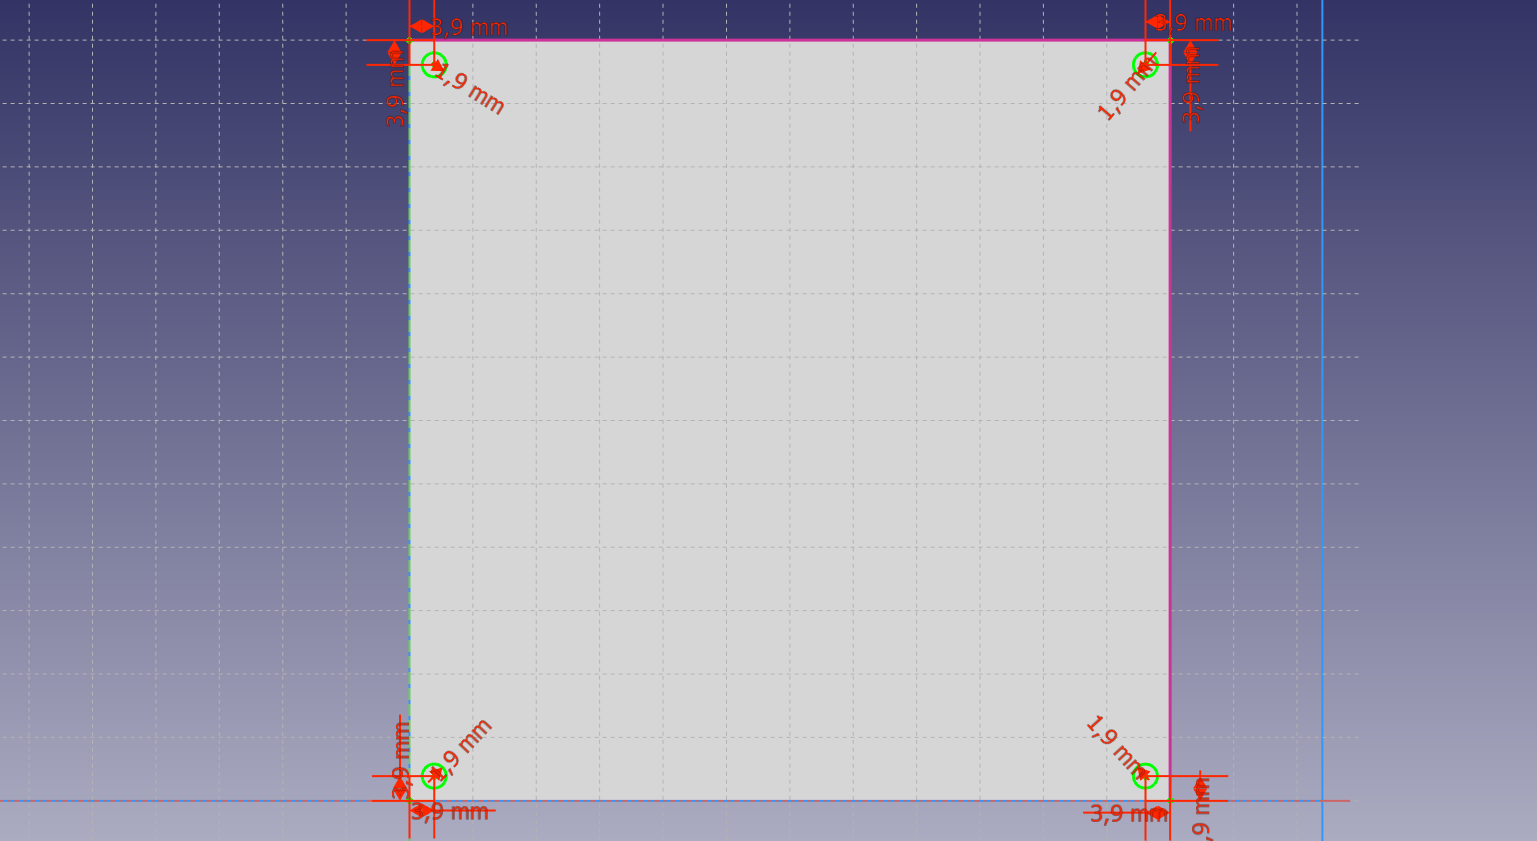
\includegraphics[width=.9\linewidth]{pictures/SketchAgujerosEsquinas.png}}
\subfigure[Detalle de una esquina]{\includegraphics[width=.9\linewidth]{pictures/DetalleAgujerosEsquinas.png}}
\caption{Agujeros para tornillos }
\label{fig:agujeros_tornillos_tapa_superior}
\end{figure}

Tras realizar los agujeros de los exteriores de la pieza, se hace un agujero central y se extruye una torre centrada sobre dicho agujero.

\begin{figure}[H]
\centering
\subfigure[Sketch del agujero central]
{\includegraphics[width=0.9\linewidth]{pictures/SketchAgujeroCentral.png}}
\subfigure[Agujero central sin torre]
{\includegraphics[width=0.9\linewidth]{pictures/AgujeroCentral.png}}
\caption{Agujeros central}
\label{fig:agujeros_central_tapa_superior}
\end{figure}

Tras definir el agujero, se extruye la torre.

\begin{figure}[H]
    \centering
    \includegraphics[width=.9\linewidth]{pictures/TorreCentral.png}
    \caption{Tapa con torre central}
    \label{fig:torre_central_tapa_superior}
\end{figure}

A continuación se procede a eliminar material de la torre con
el objetivo de disminuir la superficie de contacto con el disco rotativo y por tanto, eliminar parte del rozamiento.

\begin{figure}[H]
\centering
\subfigure[Sketch del desgaste]
{\includegraphics[width=0.9\linewidth]{pictures/SketchAnillo.png}}
\subfigure[Torre central tras el rebaje]
{\includegraphics[width=0.9\linewidth]{pictures/Anillo.png}}
\caption{Agujeros central}
\label{fig:anillo_tapa_superior}
\end{figure}

Para disminuir aun mas el rozamiento debido a posibles bordes imperfectos que queden en el disco, se realiza un chaflán en el diámetro interior y exterior.

\begin{figure}[H]
    \centering
    \includegraphics[width=.9\linewidth]{pictures/Chaflanes.png}
    \caption{Torre con chaflanes}
    \label{fig:chaflanes_tapa_superior}
\end{figure}

Finalmente se añade una ranura para que sea posible llevar los cables de los motores exteriores a la placa de control que se haya en la caja.

\begin{figure}[H]
\centering
\subfigure[Sketch de la ranura]
{\includegraphics[width=0.9\linewidth]{pictures/SketchAgujeroCables.png}}
\subfigure[Ranura para cables]
{\includegraphics[width=0.9\linewidth]{pictures/AgujeroCables.png}}
\caption{Tapa con ranura para cables}
\label{fig:ranura_cables_tapa_superior}
\end{figure}

Con esto concluimos la explicación del proceso de creación de piezas y pasamos a explicar cada una de las piezas por separado detallando los motivos por los cuales es necesario remodelar ciertas piezas y los inconvenientes y contratiempos que han surgido durante el modelado y la impresión de estas.

En primer lugar se explicará la caja que alberga la placa de control y uno de los motores.

La placa de control del brazo robótico no es la misma que en el caso del $\mu$Arm de UFACTORY. Además, los motores que se han empleado en este proyecto son servomotores con carcasa y sistema de sujeción distintos a los motores paso a paso del $\mu$Arm. Debido a estos dos factores se ha tenido que diseñar nuevas partes para la base del brazo robótico.

Mas concretamente, la necesidad de rediseñar esta parte es debida a que la base original era demasiado pequeña en superficie para permitir introducir la placa de control. Además, el servomotor no podría haber cabido junto con la placa ya que la altura era insuficiente. Por otro lado los sistemas de sujeción presentes en la caja existente no podían ser empleados para la placa de control desarrollada en este proyecto.
 
 \begin{figure}[H]
    \centering
    \includegraphics[width=.9\linewidth]{pictures/PlacaYBase.png}
    \caption{Proyección de la placa de control (naranja) sobre la base original del $\mu$Arm (gris)}
    \label{fig:placa_y_base_antiguas}
\end{figure}


 \begin{figure}[H]
    \centering
    \includegraphics[width=.9\linewidth]{pictures/PlacaMotorYParedes1.png}
    \caption{Placa y motor dentro de la caja original del $\mu$Arm}
    \label{fig:placa_motor_y_paredes1}
\end{figure}

Como se observa en la figura \ref{fig:placa_motor_y_paredes1} el motor sobresale por encima de las paredes y no hay ninguna manera de sujetarlo a estas o a la base.

Para solucionar los anteriores problemas se diseña una nueva base en la que se pueda encajar la placa, además de unas paredes lo suficientemente altas para poder introducir el motor junto con esta.

 \begin{figure}[H]
    \centering
    \includegraphics[width=.9\linewidth]{pictures/paredesybasenuevas.png}
    \caption{Base y paredes tras realizar las modificaciones necesarias}
    \label{fig:placa_y_paredes_nuevas}
\end{figure}

Inicialmente las paredes de la caja se habían diseñado con un grosor de 2mm. Tras una serie de pruebas se concluyo que dicho grosor no era suficiente para proporcionar resistencia y estabilidad suficiente, por tanto, se opto por un grosor de 3mm en la versión final.

En la base se observan los raíles que servirán para introducir y retirar la placa de la estructura. 

Se ha optado por un sistema de raíles en vez de una sujeción fia ya que de esta manera se consigue una mayor versatilidad a la hora de extraer e introducir la placa en labores de depuración y construcción. 

Además, debido al escaso espacio dentro de la caja, se hace prácticamente imposible la introducción de las herramientas necesarias para atornillar la placa a la estructura. Gracias al sistema de raíles se evita desmontar ciertas piezas al intentar introducir o extraer la placa.

Después de que la placa sea insertada en estos carriles, se asegura su posición mediante los agujeros laterales que pueden observarse en la figura \ref{fig:placa_y_paredes_nuevas}.

 \begin{figure}[H]
    \centering
    \includegraphics[width=.9\linewidth]{pictures/railes.png}
    \caption{Sistema de raíles de la placa}
    \label{fig:railes_placa}
\end{figure}

En la figura \ref{fig:railes_placa} se observan las piezas que se añadirán a la placa de control para poder deslizar esta sobre los carriles. En el exterior de la imagen aparecen los carriles presentes en la base de la caja, donde se puede ver que, al estar la placa completamente introducida en los carriles, los agujeros del carril y del raíl se posición de tal manera que se permite introducir un pasador que asegura la posición de la placa.

Debido a que tanto los raíles como los carriles se fabricaron con unas medidas teóricas, extraídas del diseño físico inicial de la placa, resulto que el ensamblaje físico no era posible.

Para solucionar este problemas se desplazaron los agujeros por los que se unía el raíl a la placa. Esto se observa en la figura \ref{fig:railes_placa_final}

 \begin{figure}[H]
    \centering
    \includegraphics[width=.9\linewidth]{pictures/RailesBien.png}
    \caption{Versión final de los carriles}
    \label{fig:railes_placa_final}
\end{figure}

Por otro lado, para poder sujetar el motor que moverá el brazo alrededor del eje vertical se ha tenido que diseñar la siguiente pieza.

 \begin{figure}[H]
    \centering
    \includegraphics[width=.9\linewidth]{pictures/sujecciónMotor.png}
    \caption{Pieza de sujeción del motor}
    \label{fig:sujecion_motor}
\end{figure}

Esta pieza se atornilla a las paredes de la caja y empleando las solapas del motor, este se atornilla en el centro de la pieza como se puede ver en la figura \ref{fig:pieza_sujecio_en_caja}.

 \begin{figure}[H]
    \centering
    \includegraphics[width=.9\linewidth]{pictures/cajaConMotor.png}
    \caption{Pieza de sujeción del motor (verde) dentro de la caja}
    \label{fig:pieza_sujecio_en_caja_resaltada}
\end{figure}

Dado que el tamaño de la base y de las paredes ha cambiado, la tapa superior debe también ser modificada para adaptar su tamaño y su sistema de sujeción a los nuevos diseños

 \begin{figure}[H]
    \centering
    \includegraphics[width=.9\linewidth]{pictures/DosTapas.png}
    \caption{Tapa original (derecha) junto a la tapa modificada (izquierda)}
    \label{fig:tapas_caja}
\end{figure}

En la figura \ref{fig:tapas_caja} se observa que en la parte superior las diferencias entre ambas piezas son mínimas respetándose los diámetros del disco exterior e interior sobre los que descansará la base giratoria.

En la figura \ref{fig:tapas_caja_con_disco} podemos observar como la base giratoria descansa sobre los anillos superiores y se inserta dentro de la tapa.

 \begin{figure}[H]
    \centering
    \includegraphics[width=.9\linewidth]{pictures/TapaSuperiorConDisco.png}
    \caption{Tapa superior transparente y base giratoria (verde)}
    \label{fig:tapas_caja_con_disco}
\end{figure}

De esta manera se consigue que el peso de la parte móvil del brazo descanse sobre la tapa y no sobre el eje de rotación. Por otro lado, el hecho de que la base giratoria protruya hacia el interior de la tapa permite que la pieza este mas cerca del motor permitiendo acortar el eje.

A en la figura \ref{fig:cilindro_con_pletina} se muestra la pieza que conecta el motor a la base giratoria a través de un eje. Esta pieza tiene en su base un desgaste tal que permite que el engranaje del motor pueda ser introducido dentro, mientras que en la parte de arriba tiene unos agujeros que permiten la sujeción de un eje metálico el cual llega hasta la base giratoria y transmite el movimiento del motor a esta.

La pieza plana que protruye hacia un lateral sirve para que el cilindro pueda alcanzar un fin de carrera que indique cuando el motor ha llegado a una posición extrema.

\begin{figure}[H]
    \centering
    \includegraphics[width=.9\linewidth]{pictures/CilindroConPletina.png}
    \caption{Pieza de unión del motor y el eje}
    \label{fig:cilindro_con_pletina}
\end{figure}

\begin{figure}[H]
    \centering
    \includegraphics[width=.9\linewidth]{pictures/SistemaCompleto.png}
    \caption{Sistema completo}
    \label{fig:sistema_completo}
\end{figure}

En la figura \ref{fig:sistema_completo} se observa la construcción completa de la base. En esta imagen se dejan las paredes y la tapa superior con cierta transparencia para poder ver el interior de la caja. Entre el cilindro montado encima del motor y la base giratoria habrá un eje metálico que comunicara el movimiento.

Por otro lado, para que sea posible ubicar los motores que se encargaran del movimiento vertical del brazo se han de crear nuevas piezas en las que puedan ser atornillados. Esta pieza puede observarse en la figura \ref{fig:pletina_sujecion_motor}

\begin{figure}[H]
    \centering
    \includegraphics[width=.9\linewidth]{pictures/pletina_motor.png}
    \caption{Placa de sujeción de los motores laterales}
    \label{fig:pletina_sujecion_motor}
\end{figure}

En fases mas avanzadas del proyecto, el equipo de desarrollo observo tras realizar pruebas, que el eje metálico no podía ser asegurado en el centro del cilindro (Mas detalles en el apartado \ref{pruebas_post_impresión}). También concluyó que en determinadas configuraciones geométricas del brazo, este podía ejercer demasiada fuerza sobre el eje de giro horizontal.

Por ello se tuvieron que realizar los siguientes cambios.

En el disco rotativo se añadió un carril que encajara en la ranura de la tapa superior. El cometido de este carril es evitar movimientos en el plano horizontal, dar mejor soporte ante el peso y ayudar a guiar el movimiento.

\begin{figure}[H]
    \centering
    \includegraphics[width=.9\linewidth]{pictures/TapaConBaseRotatoria.png}
    \caption{Base de giro con raíl}
    \label{fig:base_de_giro_con_rail}
\end{figure}

Para evitar emplear un eje metálico, el equipo de desarrollo diseña una pieza que pueda ser acoplada a la base giratoria1.

\begin{figure}[H]
    \centering
    \includegraphics[width=.9\linewidth]{pictures/EjeMadeInElEquipoDeDesarrollo.png}
    \caption{La pieza sustituta del eje metálico (naranja)}
    \label{fig:pieza_sustituta_eje}
\end{figure}

Según se observa en la figura \ref{fig:pieza_sustituta_eje} la base giratoria y la parte que servirá para sustituir al eje metálico, serán unidas mediante dos tornillos.
También se puede observar el carril de la base rotatoria en una perspectiva ascendente.

\begin{figure}[H]
    \centering
    \includegraphics[width=.9\linewidth]{pictures/CadenaCineticaDelEje.png}
    \caption{Sistema completo del eje giratorio}
    \label{fig:sistema_completo_eje}
\end{figure}

En la imagen \ref{fig:sistema_completo_eje} se puede observar la ultima pieza del sistema. Su cometido es servir como engranaje sobre el eje del motor y por tanto transmitir el movimiento a las piezas superiores.
Será unida a la pieza superior mediante 4 tornillos.

Otra pieza que tuvo que ser modificada es la sujeción del \textit{end--efector}.

\begin{figure}[H]
    \centering
    \includegraphics[width=.9\linewidth]{pictures/EndEffectorModificado.png}
    \caption{\textit{End--effector} inicial (izquierda). \textit{End--effector} modificado (derecha)}
    \label{fig:end_effector_modificado}
\end{figure}

Como se puede observar en la figura \ref{fig:end_effector_modificado}, la modificación consiste en la adición de un refuerzo en las partes menos resistentes. 
Esta pieza fue modificada tras observar la fragilidad de las paredes laterales cuando estas se rompieron en la pieza sin refuerzo.

Cabe destacar que, pese a que una gran parte de las piezas no han sido mencionadas de manera concreta en este apartado, todas ellas han sido revisadas de manera individual y han sido editadas para posibilitar el uso de los tornillos, rodamientos y ejes disponibles.

Mas concretamente, los tornillos de 4x16 en el caso de las piezas que han sido construidas desde cero por parte del equipo de desarrollo, y tornillos de 3x10 y 3x20 según el caso, en piezas editadas.

En ultimo lugar se han adaptado las ranuras para los rodamientos de 8mm de diámetro externo que han sido adquiridos para el proyecto.

Tras añadir dichas piezas al diseño general y completar este con las piezas originales que no han sido modificados obtenemos el diseño definitivo del brazo robotico el cual se puede observar en la figura \ref{fig:brazo_completo_modificado}.

\begin{figure}[H]
    \centering
    \includegraphics[width=.9\linewidth]{pictures/BrazoEntero.png}
    \caption{Brazo robotico completo tras las modificaciones}
    \label{fig:brazo_completo_modificado}
\end{figure}
\section{Construcción del brazo}
A continuación se procede a explicar la construcción del brazo robotico. Para ello, se emplearán los diseños 3D y ciertas imágenes del brazo real en sus etapas de construcción.

La razón de no explicar el proceso integro con imágenes reales del brazo es debido a que no hay suficientes documentos gráficos para ejemplificar el proceso completo y ciertas etapas de la construcción quedarían sin poder ser documentadas.

\begin{figure}[H]
    \centering 
    \includegraphics[width=1\linewidth]{pictures/ElementosMecanicosExternos.jpg}
    \caption{Elementos mecánicos externos}
    \label{fig:elementos_mecanicos_externos}
\end{figure}

En la figura \ref{fig:elementos_mecanicos_externos} se pueden observar los distintos tornillos, tuercas y arandelas que se emplearan a lo largo de la construcción del brazo. Esta imagen puede servir como referencia para tener una imagen real de los diferentes elementos externos que se nombrarán a lo largo de la explicación.

\begin{figure}[H]
    \centering 
    \includegraphics[width=1\linewidth]{pictures/BaseDelBrazoRobotico.png}
    \caption{Base de la caja del brazo robótico}
    \label{fig:base_caja_brazo_robotico}
\end{figure}

\begin{figure}[H]
    \centering 
    \includegraphics[width=1\linewidth]{pictures/BaseYParedes.png}
    \caption{Base y paredes de la caja del brazo robótico}
    \label{fig:base_paredes_caja_brazo_robotico}
\end{figure}

\begin{figure}[H]
    \centering 
    \includegraphics[width=1\linewidth]{pictures/CajaCompleta.png}
    \caption{Caja completa del brazo robótico}
    \label{fig:caja_completa_brazo_robotico}
\end{figure}

Como observamos en las figuras \ref{fig:base_caja_brazo_robotico}, \ref{fig:base_paredes_caja_brazo_robotico} y \ref{fig:caja_completa_brazo_robotico} la caja esta compuesta por 3 piezas y estas se ensamblan verticalmente una encima de otra mediante tornillo de 4x15 cm.
Cabe destacar que esta parte de la estructura es inmóvil y sirve como soporte para la parte móvil.

\begin{figure}[H]
    \centering 
    \includegraphics[width=1\linewidth]{pictures/MotorHold.png}
    \caption{Sujeción del motor de la base}
    \label{fig:sujección_motor_base}
\end{figure}

\begin{figure}[H]
    \centering 
    \includegraphics[width=1\linewidth]{pictures/MotorHoldYMotor.png}
    \caption{Motor de la base ensamblado en su soporte}
    \label{fig:motor_ensamblado_soporte}
\end{figure}

\begin{figure}[H]
    \centering 
    \includegraphics[width=1\linewidth]{pictures/MotorMasPrimeraPieza.png}
    \caption{Primera pieza del sistema de transmisión del movimiento}
    \label{fig:primera_pieza_sistema_transmision}
\end{figure}

\begin{figure}[H]
    \centering 
    \includegraphics[width=1\linewidth]{pictures/MotorMasSegundaPieza.png}
    \caption{Segunda pieza del sistema de transmisión del movimiento}
    \label{fig:segunda_pieza_sistema_transmision}
\end{figure}

\begin{figure}[H]
    \centering 
    \includegraphics[width=1\linewidth]{pictures/MotorMasTerceraPieza.png}
    \caption{Tercera pieza del sistema de transmisión del movimiento}
    \label{fig:tercera_pieza_sistema_transmision}
\end{figure}

\begin{figure}[H]
    \centering 
    \includegraphics[width=1\linewidth]{pictures/FinalDeCarrera.png}
    \caption{Cadena de transmisión final con soporte para fin de carrera}
    \label{fig:sistema_transmision_fin_carrera}
\end{figure}

En las figuras \ref{fig:sujección_motor_base}, \ref{fig:motor_ensamblado_soporte}, \ref{fig:primera_pieza_sistema_transmision},
\ref{fig:segunda_pieza_sistema_transmision},
\ref{fig:tercera_pieza_sistema_transmision} y \ref{fig:sistema_transmision_fin_carrera} se observan los componentes que servirán para transmitir el movimiento desde el motor a la base giratoria donde ira ensamblado el brazo robótico. Para asegurar el soporte a las paredes y posteriormente el motor al soporte se han empleado tornillos de 4x15 mm. Para los componentes que servirán para transmitir el movimiento, se han empleado tornillos de 3x10 mm debido a que las piezas son mas pequeñas y es necesario que los tornillos ocupen menos espacio.

\begin{figure}[H]
    \centering 
    \includegraphics[width=1\linewidth]{pictures/CajaConPiezasInternas.png}
    \caption{Interior de la caja}
    \label{fig:interior_caja_sujeccion}
\end{figure}

Sobre la base giratoria superior será montado ahora el sistema de motores que se encargará de mover el brazo en el eje vertical.

\begin{figure}[H]
    \centering 
    \includegraphics[width=1\linewidth]{pictures/BaseRotatoriaConPletinas.png}
    \caption{Base rotatoria con pletinas}
    \label{fig:base_rotatoria_pletinas}
\end{figure}

En la figura \ref{fig:base_rotatoria_pletinas} se observa que las pletinas que sujetaran los motores a la base encajan en las hendiduras que existen en la base rotatoria. Estas pletinas son aseguradas a la base giratoria mediante tornillos 3x6 mm.

\begin{figure}[H]
    \centering 
    \includegraphics[width=1\linewidth]{pictures/BaseRotatoriaConPletinasYSoporte.png}
    \caption{Soporte para los motores laterales}
    \label{fig:soporte_motores_laterales}
\end{figure}

A continuación los soportes de los motores son añadidos a las pletinas y son asegurados a estas mediante tornillos de 4x15 mm con tuerca y arandela.
Entre la pletina y el soporte se puede observar una pequeña distancia, la cual se debe a un separador que existe en la construcción real pero que no aparece en el diseño 3D.

\begin{figure}[H]
    \centering 
    \includegraphics[width=1\linewidth]{pictures/BaseRotatoriaConUnMotor.png}
    \caption{Se añade uno de los motores}
    \label{fig:un_motor_añadido}
\end{figure}

Finalmente uno de los motores es añadidos a su soportes y es asegurado a este mediante tornillos de 4x10 mm con tuerca.

Por otro lado, es ensamblada la parte superior del del brazo según se indica a continuación.

\begin{figure}[H]
    \centering 
    \includegraphics[width=1\linewidth]{pictures/SegmentoCentralBrazo.png}
    \caption{Segmento central del brazo robótico}
    \label{fig:segmento_central_brazo}
\end{figure}

\begin{figure}[H]
    \centering 
    \includegraphics[width=1\linewidth]{pictures/SoporteMotorIzquierdo.png}
    \caption{Pieza izquierda de la cadena de movimiento vertical}
    \label{fig:pieza_izquierda_brazo}
\end{figure}

En las figuras \ref{fig:segmento_central_brazo} y \ref{fig:pieza_izquierda_brazo} se observa el montaje de la primera pieza de la cadena de movimiento vertical sobre el segmento central del brazo. Para asegurar la pieza al brazo se emplean tornillos 3x6 mm .

\begin{figure}[H]
    \centering 
    \includegraphics[width=1\linewidth]{pictures/SoporteMotorCentral.png}
    \caption{Pieza central de la cadena de movimiento vertical}
    \label{fig:pieza_central_brazo}
\end{figure}

En la figura \ref{fig:pieza_central_brazo} se monta la pieza central empleando los mismos tornillos de tamaño 3x6 mm.

\begin{figure}[H]
    \centering 
    \includegraphics[width=1\linewidth]{pictures/SoporteMotorDerecho.png}
    \caption{Pieza derecha de la cadena de movimiento vertical}
    \label{fig:pieza_derecha_brazo}
\end{figure}

Finalmente se añade la pieza derecha según se observa en la figura \ref{fig:pieza_derecha_brazo}. Esta ultima es soportada por un eje metálico que atraviesa las 3 piezas.

En la parte superior del segmento central se monta una pieza según se observa en la figura \ref{fig:pieza_forma_rara}

\begin{figure}[H]
    \centering 
    \includegraphics[width=1\linewidth]{pictures/PiezaConFormaRara.png}
    \caption{Pieza que sirve para unir el segmento inferior con el superior}
    \label{fig:pieza_forma_rara}
\end{figure}

Esta pieza se moverá de manera libre sobre un tornillo 4x15 mm que la atraviesa a modo de eje y que apoya sobre el segmento inferior en dos rodamientos los cuales se encuentran el las ranuras circulares que se observan en la figura \ref{fig:pieza_forma_rara}

Empleando esta pieza es posible asegurar el antebrazo en posición según se ve en la figura \ref{fig:antebrazo}. También se pueden apreciar los rodamientos de los que se hablaba en el párrafo anterior.

\begin{figure}[H]
    \centering 
    \includegraphics[width=1\linewidth]{pictures/Antebrazo.png}
    \caption{Antebrazo montado en la cadena articulada principal}
    \label{fig:antebrazo}
\end{figure}

Finalmente se añade a la cadena articulada principal el soporte del \textit{end--effector} según se observa en la figura \ref{fig:soporte_endeffector}. Este se mantiene unido al antebrazo mediante un tornillo de 4x15 mm el cual sirve de eje libre que lo atraviesa y se apoya en los dos rodamientos que se observan de color naranja en la figura.

\begin{figure}[H]
    \centering 
    \includegraphics[width=1\linewidth]{pictures/SoporteEndEffector.png}
    \caption{Soporte del \textit{end--ffector}}
    \label{fig:soporte_endeffector}
\end{figure}

También se añade al soporte del \textit{end--efector} la sujeción para un posible motor que podría operar una pinza. Esto se puede ver en \ref{fig:soporte_motor}. Para asegurar esta pieza sobre el soporte, se emplean tornillos de 3x6 mm.

\begin{figure}[H]
    \centering 
    \includegraphics[width=1\linewidth]{pictures/SujecionMotorFinal.png}
    \caption{Soporte del motor que actúa sobre el \textit{end--effector}}
    \label{fig:soporte_motor}
\end{figure}

Llegados a este punto es preciso ensamblar las cadenas articuladas auxiliares las cuales permiten transmitir movimientos al antebrazo y al \textit{end--efector}.

Primero se ensambla la cadena auxiliar derecha según se observa en la figura \ref{fig:auxiliar_derecha}

\begin{figure}[H]
    \centering 
    \includegraphics[width=1\linewidth]{pictures/CadenaArticuladaDerecha.png}
    \caption{Cadena articulada auxiliar derecha}
    \label{fig:auxiliar_derecha}
\end{figure}

La cadena auxiliar derecha se compone de una sola varilla que se ensambla en una de las piezas de la cadena de movimiento vertical, en la parte inferior del brazo, mediante un tornillo de 4x10 mm. En la parte superior la varilla se ensambla en la junta de unión del brazo con el antebrazo mediante un tornillo de 4x15 mm. Se puede observar que en ambos casos para permitir que los tornillos actúen como eje libre, estos se apoyan sobre rodamientos.

En segundo lugar se ensambla la cadena auxiliar izquierda. Se empieza añadiendo el triangulo de unión de las dos varillas que se explicarán mas adelante. Este triangulo se observa en la figura \ref{fig:triangulo_union_varillas}

\begin{figure}[H]
    \centering 
    \includegraphics[width=1\linewidth]{pictures/TrianguloDeUnion.png}
    \caption{Triangulo de unión del las varillas de la cadena auxiliar izquierda}
    \label{fig:triangulo_union_varillas}
\end{figure}

Este triangulo se sujeta sobre el mismo eje que la junta de unión.
Se observa en azul un separador y en naranja el rodamiento gracias al cual se consigue que el tornillo sirva como eje libre.

Sobre este triangulo se añade una primera varilla que une el triangulo con uno de los soportes de los motores de la base, esta varilla se observa en la figura \ref{fig:varilla_inferior_izquierda}

\begin{figure}[H]
    \centering 
    \includegraphics[width=1\linewidth]{pictures/VarillaInferior.png}
    \caption{Varilla inferior de la cadena auxiliar izquierda}
    \label{fig:varilla_inferior_izquierda}
\end{figure}

Esta varilla se sujeta en el triangulo mediante un tornillo de 4x10 mm el cual apoya sobre un rodamiento que hace que sirva de eje libre. En el soporte inferior del motor se sujeta mediante un tornillo de 4x40 mm.

Finalmente se une la varilla superior con el \textit{end--efector} mediante un tornillo de 4x10 mm y un rodamiento. En el triangulo se emplea el mismo método de sujeción. Esto se puede observar en la imagen \ref{fig:varilla_superior_izquierda}

\begin{figure}[H]
    \centering 
    \includegraphics[width=1\linewidth]{pictures/VarillaSuperior.png}
    \caption{Varilla superior de la cadena auxiliar izquierda}
    \label{fig:varilla_superior_izquierda}
\end{figure}

Con esto finalizamos la construcción de la parte superior del brazo robótico y ya es posible introducirlo en la base rotatoria.

\begin{figure}[H]
    \centering 
    \includegraphics[width=1\linewidth]{pictures/ParteSuperiorDelBrazoEnElSoporte.png}
    \caption{La parte superior el brazo robótico ensamblada en la base rotativa.}
    \label{fig:parte_superio_ensamblada_base}
\end{figure}

Finalmente se coloca el ultimo motor y se deja la parte superior del brazo fijada entre los dos 





%% REVISADO
\section{Configuración mecánica del brazo}
La estructura del brazo es pantográfica, lo cual significa que es un sistema de enlaces mecánicos que reproduce el movimiento de un punto de una articulación en un segundo punto, normalmente a un tamaño o bien más pequeño o bien más grande, como se puede apreciar en la figura \ref{fig:estrucutra_pantografica}. Se originó en el siglo XVII y su aplicación más conocida es como instrumento de dibujo.

\begin{figure}[H]
    \centering
    \includegraphics[width=.7\linewidth]{pictures/link-to-elliott-p149-suspended-pantograph-sf0.jpg}
    \caption{Una estructura pantográfica que transmite el movimiento de un punto al siguiente \cite{PantographContext}.}
    \label{fig:estrucutra_pantografica}
\end{figure}

El hecho de que que la estructura del brazo sea pantográfica permite controlar todas las articulaciones mediante motores ubicados en la base. Esto es de especial importancia ya que hace posible que las articulaciones finales no carguen con el peso de los motores, permitiendo emplear materiales como el plástico para la construcción de la estructura y, además, dando capacidad al brazo para levantar cargas más pesadas.

Otro beneficio derivado de la ubicación de los motores en la base es la alta estabilidad del brazo, ya que siendo estos los componentes más pesados y estando ubicados en la base se consigue un centro de gravedad muy cercano a la superficie de apoyo, permitiendo así un amplio rango de movimientos, como se puede ver en la figura \ref{fig:pArm_working_area}.

\begin{figure}[H]
    \centering
    \includegraphics[width=.6\linewidth]{pictures/arm_weights_distances.png}
    \caption{Área de trabajo de \pArm{} \cite{UFACTORYXArmTextbackslashtextbaruArm}.}
    \label{fig:pArm_working_area}
\end{figure}

Otra característica a destacar es que debido a la estructura pantográfica, el \textit{end--effector} mantiene siempre un ángulo perpendicular con la superficie de apoyo del brazo. Esto supone, por un lado, perder ciertos grados de libertad pero por otro, simplificar la estructura y abaratar el coste de producción.
%% REVISADO
\section{Microcontrolador utilizado}
Para el desarrollo del la placa que conforma el S2 se ha empleado un microcontrolador dsPIC33EP512GM604.
Los motivos por los cuales se ha usado este modelo de DSP son los siguientes: 

\begin{itemize}
\item En primera instancia, a la cantidad y a la precisión de los PWM que este ofrece, ya que son suficientes para poder controlar todos los motores y además su precisión permite generar una señal adecuada para controlar cada uno de los motores.

\item Por otro lado, debido a la naturaleza de los cálculos que se deben realizar para convertir posiciones cartesianas a ángulos y viceversa, el DSP facilita el calculo de las diferentes operaciones matriciales que permiten esta conversión.

\item Otro aspecto importante es la posibilidad de almacenar hasta 512KB de memoria de programa.

\item Por ultimo se ha elegido un DSP Microchip debido a que todos los integrantes del grupo de desarrollo tiene experiencia previa con este fabricante. Además, dicho fabricante proporciona documentación extensa sobre sus productos.

\end{itemize}

Una parte critica del proyecto es la precisión y el control de los motores. En este aspecto los PWM del DSP permiten generar ciclos de trabajo a partir de un registro de 16 bits. Para una frecuencia de 50hz (Periodo de 20ms), un giro de 360 grados supondría una duración del nivel alto de 5ms. Es decir que se podrá controlar la rotación entre 0 y 360 grados con $ 2^{16}/4 = 16384$ bits esto supone que obtendremos una precisión máxima de $360/16384 = 0,02197 grados$ que es suficiente para el proyecto.

En cuanto a las operaciones matemáticas el DSP cuenta con un circuito PLL (Phase Loop Lock) el cual permite incrementar la frecuencia del oscilador para conseguir de esta manera una mayor cantidad de microinstrucciones por segundo y por tanto un mayor volumen de operaciones.

Debido a la complejidad del proyecto y a la gran variedad de sistemas que debemos emplear el código de programa es considerablemente grande. 512KB son suficientes para almacenar la memoria de programa para este proyecto.

Este microcontrolador gracias a que dispone de puertos UART permite recibir las ordenes y los movimientos necesarios desde el S1, por otro lado, el DSP cuenta con un PLL el cual permite aumentar la frecuencia interna del microcontrolador para incrementar la cantidad de operaciones por segundo que este puede hacer. Después de realizar las operaciones este se encargará de generar las señales PWM necesarias para mover los motores de tal manera que el brazo robótico quede en la posición deseada.





    

%% REVISADO
\section{Desarrollo y componentes de la PCB}
\subsection{Objetivos}

El desarrollo de una PCB se considera una de las partes esenciales de este proyecto y por lo tanto su importancia es máxima.

El objetivo principal que persigue el diseñar y construir una PCB en este proyecto es el de dotar al sistema de un centro de cómputo principal, el cual es utilizado para procesar las ordenes de S1, realizar los cálculos pertinentes y ejecutar las acciones necesarias sobre la estructura del brazo robótico.

Se considera  por lo tanto que la PCB es el centro de computo principal del sistema y por lo tanto se encarga de alojar el microcontrolador DSPIC, así como todos los periféricos necesarios para establecer la comunicación con S1, realizar el control de los actuadores y monitorizar el estado del manipulador.

En los siguientes apartados se detalla el proceso de diseño y construcción llevado a cabo para completar la PCB.

\subsection{Componentes principales}

El diseño de la PCB esta completamente estructurado según varios componentes principales, por lo tanto, en este apartado se describe cuales son, las decisiones que han llevado a incluirlos y sus funcionalidades principales dentro del proyecto.

En general se podría decir que los componentes de la PCB se clasifican en tres categorías principales:
\begin{itemize}
    \item Componentes de alimentación eléctrica.
    \item Microcontrolador y componentes auxiliares para su correcto funcionamiento.
    \item Periféricos destinados a control de actuadores y canales de comunicación.
\end{itemize}

En primer lugar, los componentes de alimentación eléctrica son aquellos que forman el circuito de alimentación del microcontrolador así como de los actuadores. El circuito eléctrico de alimentación de la PCB se ha diseñado para poder alimentar de forma simultánea al microcontrolador y a cada uno de los cuatro servomotores y por lo tanto, está formado por dos etapas:
\begin{itemize}
    \item La PCB recibe una tensión de entrada de 9V y una corriente de entre 1.8A - 2A mediante una clema. Posteriormente esta tensión de alimentación será reducida y adaptada para alimentar a cada una de las etapas de la PCB, es decir, al microcontrolador y servomotores.
    \item En la primera etapa se reduce el voltaje de alimentación principal a 6V y 0.4A aproximadamente para cada uno de los servomotores, utilizando para ello un regulador LM317 para cada servomotor. Esta alimentación se realiza mediante clemas, a las cuales se deben conectar la alimentación de los motores.
    \item En la segunda etapa se reduce el voltaje de alimentación principal a 3.3V y 0.15A aproximadamente con objetivo de alimentar el microcontrolador, utilizando para  ello un regulador LM317. Esta alimentación se realiza mediante pistas únicamente.
\end{itemize}

En segundo lugar, el microcontrolador y sus componentes auxiliares representan el núcleo de la PCB:
\begin{itemize}
    \item El DSPIC se encuentra localizado en el centro de la PCB y de él surgen todas las conexiones necesarias hacia los periféricos.
    \item Los componentes auxiliares del microcontrolador son componentes eléctricos que aseguran el correcto funcionamiento del DSPIC, así como su seguridad. En el caso específico de este microcontrolador, es necesario incluir varios condensadores en sus pines de alimentación.
\end{itemize}

En último lugar se detallan los principales periféricos que serán empleados:
\begin{itemize}
    \item Cristal de cuarzo: mediante este periférico se genera una señal de reloj precisa y de buena calidad, su frecuencia es de 7Mhz y sera recibida por el microcontrolador para ser usada como señal de reloj principal del sistema.
    \item Puerto de programación: mediante este periférico se puede conectar la sonda de programación del microcontrolador y por lo tanto es un elemento esencial.
    \item Puerto TRIS: mediante este periférico se pueden recibir señales digitales y analógicas las cuales son procesadas por el microcontrolador. En este proyecto se utiliza este periférico para monitorizar los finales de carrera de la estructura del brazo robótico.
    \item Puerto PWM: mediante este periférico se pueden generar señales PWM, las cuales son completamente necesarias para controlar los servomotores.
    \item UART: mediante este periférico se establece un canal de comunicación hardware con S1, el cual se usa para recibir ordenes, movimientos y realimentar su resultado de vuelta a S1.
    \item LEDS de estado: mediante este periférico se muestra el estado del sistema usando tres diodos LED.
\end{itemize}

Mediante esta descripción general de la PCB y sus componentes se pretende brindar una idea global de la misma, así como de cual es su papel dentro del proyecto. En los apartados siguientes se describe en términos técnicos los elementos de esta PCB, así como el proceso de diseño y fabricación llevado a cabo.

\subsection{Diseño lógico y diagrama esquemático}

El primer paso llevado a cabo durante el diseño de la PCB ha sido realizar un diseño lógico de alto nivel, en el cual se muestran las conexiones lógicas que existen entre los componentes; se trata por lo tanto del diseño con mayor nivel de abstracción y que tiene como objetivo establecer un diseño de primer nivel, es decir, la primera toma de contacto con el plano de la PCB.

El diseño lógico se lleva a cabo mediante un diagrama esquemático que contiene dos tipos de elementos: huella lógica de cada uno de los componentes y conexiones entre ellos. Este diagrama se ha llevado a cabo utilizando la herramienta Schematic Layout Editor incluida en KiCad.

El diagrama esquemático esta dividido en dos partes principales, las cuales facilitan la compresión del mismo:
\begin{itemize}
    \item Diagrama esquemático del circuito de alimentación.
    \item Diagrama esquemático del microcontrolador y sus periféricos.
\end{itemize}

En primer lugar se procede a describir detalladamente el diagrama esquemático del circuito de alimentación, el cual contiene las dos etapas de alimentación, siendo los principales componentes usados los reguladores de voltaje LM317,L7805CV y AZ1117H.

La clema principal de alimentación recibe 9V y 1.8A aproximadamente. Esta alimentación debe ser provista externamente mediante una fuente de alimentación regulable o similares. 

Conectados directamente a la clema principal se encuentran conectados los reguladores de tensión correspondientes a las dos etapas de alimentación:
\begin{itemize}
    \item La primera etapa de alimentación está formada por cuatro reguladores LM317, los cuales alimentan cada uno de los servomotores. En esta etapa de alimentación se reduce el voltaje de 9V a 5.5V.
    
    \item La segunda etapa de alimentación está formada por un regulador de tensión L7805CV y un AZ1117H. En esta etapa de alimentación se reduce el voltaje de 9V a 5V usando el primer regulador, y de 5V a 3.3V usando el segundo.
\end{itemize}

El funcionamiento del regulador LM317 es bastante común, se trata de un regulador de voltaje ajustable que recibe una tensión continua de entrada de entre 3V - 40V, y provee una tensión continua salida de entre 1.25V - 37V; la relación entre la tensión de entrada y salida depende de dos resistencias auxiliares. El conexionado sugerido por el fabricante es el siguiente y se ha obtenido del datasheet del regulador:

\begin{figure}[H]
    \centering 
    \includegraphics[width=.6\linewidth]{pictures/Lm317 conexionado.PNG}
    \caption{Diagrama de conexionado.}
    \label{fig:kdiagram}
\end{figure}


La ecuación de funcionamiento del regulador que ofrece el fabricante es la siguiente:
\begin{equation}
    V_{OUT} = V_{REF} \cdot \left( 1 + \frac{R2}{R1}\right) + I_{ADJ} \cdot R2
\end{equation}

La ecuación anterior debe ser usada para realizar los cálculos pertinentes sobre el valor de las resistencias R2 y R1. Se pueden realizara además dos observaciones necesarias para la correcta aplicación de la ecuación anterior:
\begin{itemize}
    \item Se tiene que por definición, el fabricante establece el valor $V_{REF}$ en 1.25V
    \item Por motivos de construcción del regulador, la corriente $I_{ADJ}$ tiene un valor máximo de $100 \mu A$ y por lo tanto el término de la ecuación que la involucra puede ser despreciado.
\end{itemize}

Se tiene por lo tanto que la ecuación funcional a utilizar en el cálculo de R1 y R2 es:

\begin{equation}
    V_{OUT} = 1.25 \cdot \left( 1 + \frac{R2}{240}\right) 
\end{equation}

Teniendo en cuenta los voltajes de alimentación requeridos para las dos etapas de alimentación de la PCB, se han realizado los siguientes cálculos para los valores de la resistencia R1 y R2:
\begin{itemize}
    \item Primera etapa, alimentación de servomotores, 5.5V y 0.4A requeridos:
    \begin{equation}
        5.5 = 1.25 \cdot \left( 1 + \frac{R2}{R1}\right) 
    \end{equation}
    Por disponibilidad de materiales, se ha decidido escoger los valores $150 \Omega$ y $500 \Omega$ para los valores de R1 y R2 respectivamente. Tomando en cuenta dichos valores y utilizando la ecuación anterior, se obtiene una reducción de voltaje de 9V a 5.41V, voltaje suficiente para alimentar los servomotores.
\end{itemize}

Aplicando el conexionado recomendado por el fabricante y los cálculos para el valor de las resistencias se obtiene finalmente el diagrama esquemático del circuito de alimentación de los servomotores:

\begin{figure}[H]
    \centering 
    \includegraphics[width=.85\linewidth]{pictures/EsquematicoAlimentaciónServos.PNG}
    \caption{Diagrama esquemático del circuito de alimentación de los servomotores}
    \label{fig:kdiagram}
\end{figure}

El funcionamiento de los reguladores L7805CV y AZ1117H es simple:
\begin{itemize}
    \item El regulador L7805CV recibe un voltaje de entre 7V - 35V y provee un voltaje de salida fijo de 5V. Su conexionado se realiza utilizando dos condensadores auxiliares, tal y como se describe en el datasheet del componente:
    
    \begin{figure}[H]
    \centering 
    \includegraphics[width=.75\linewidth]{pictures/L7805Datasheet.PNG}
    \caption{Diagrama de conexionado del regulador L7805}
    \label{fig:kdiagram}
    \end{figure}
    
    \item El regulador AZ1117H recibe un voltaje de hasta 15V y provee un voltaje de salida fijo de 3.3V. Su conexionado se realiza de la misma forma que para el regulador anterior, tal y como se describe en el datasheet del componente:
    
    \begin{figure}[H]
    \centering 
    \includegraphics[width=.75\linewidth]{pictures/AZ1117Hdatasheet.PNG}
    \caption{Diagrama de conexionado del regulador AZ1117H}
    \label{fig:kdiagram}
    \end{figure}
    
    En el diagrama anterior se utiliza el modelo que ofrece regulación de voltaje a 5V, sin embargo el modelo usado en el proyecto es el que ofrece regulación de voltaje a 3.3V, siendo su conexionado exactamente igual.
    
\end{itemize}

Teniendo en cuenta la información expuesta anteriormente, se ha decidido conectar en serie ambos reguladores, consiguiendo de esta forma una regulación de 9V a 5V y posteriormente una regulación de 5V a 3.3V. El diagrama esquemático final es el siguiente:

    \begin{figure}[H]
    \centering 
    \includegraphics[width=.95\linewidth]{pictures/EsquematicoAlimentaciónPic.PNG}
    \caption{Diagrama esquemático de la etapa de alimentación del microcontrolador}
    \label{fig:kdiagram}
    \end{figure}

Es importante destacar tres aspectos:
\begin{itemize}
    \item La primera etapa de alimentación incluye clemas para su conexionado con los servomotores.
    \item La segunda etapa de alimentación incluye un puerto de cuatro pines, los cuales se usan para alimentar los micro-interruptores y el microcontrolador.
    \item El conexionado de todos los reguladores se ha realizado en paralelo, dedicando un regulador para cada servomotor, así como para el microcontrolador. El objetivo de esta configuración es garantizar una vía de alimentación independiente para cada componente, reduciendo las interferencias de alimentación entre los reguladores y, diferenciando la etapa de alimentación de los servomotores y microcontrolador.
\end{itemize}

En segundo lugar se procede a describir detalladamente el diagrama esquemático del microcontrolador y sus periféricos. A continuación se muestra el diagrama esquemático final y posteriormente se detallará cada uno de los periféricos:

\begin{figure}[H]
    \centering 
    \includegraphics[width=.95\linewidth]{pictures/EsquematicoMicrocontrolador.PNG}
    \caption{Diagrama esquemático del microcontrolador y sus periféricos}
    \label{fig:kdiagram}
\end{figure}

Primeramente es importante describir los condensadores auxiliares necesarios para el correcto funcionamiento del microcontrolador, los cuales se encuentran conectados en los pines de alimentación del mismo. Su conexionado es sugerido por el fabricante en el datasheet según el siguiente esquema, se trata de la configuración mínima recomendada:

\begin{figure}[H]
    \centering 
    \includegraphics[width=.7\linewidth]{pictures/Minimun.PNG}
    \caption{Conexionado mínimo del microcontrolador}
    \label{fig:kdiagram}
\end{figure}

Todos los condensadores han sido conectados a los pines descritos por el fabricante y escogidos teniendo en cuenta las características técnicas de los mismos, también descritas en el datasheet.

A continuación se describe el conexionado del resto de puertos y periféricos:

\begin{itemize}
    \item Cristal de cuarzo: se trata del periférico que genera la señal de reloj principal del sistema, en este caso, su frecuencia es de 7.3728 Mhz y entra dentro del rango de válido mencionado en el datasheet.
    
    \begin{figure}[H]
    \centering 
    \includegraphics[width=.7\linewidth]{pictures/Cristal.PNG}
    \caption{Diagrama esquemático del conexionado del generador de señales}
    \label{fig:kdiagram}
    \end{figure}
    
    Su conexionado se realiza con los pines 32 y 31 del microcontrolador, siguiendo la estructura de la imagen anterior, empleando también una resistencia de $1 M \Omega$ y dos condensadores de 22 pF.
    
    \item Puerto de programación mediante sonda: se trata del puerto que permite conectar la sonda que introduce el código a ejecutar en el microcontrolador.
    
    El conector que recibe la sonda debe tener una estructura específica y se describe en el datasheet de la misma:
    
    \begin{figure}[H]
    \centering 
    \includegraphics[width=.5\linewidth]{pictures/Sonda.PNG}
    \caption{Pinout del conector de la sonda de programación}
    \label{fig:kdiagram}
    \end{figure}
    
     Cabe destacar que el pin 18 o MCLR debe tener un conexionado específico en el que se emplea una resistencia pull-up; esta estructura de conexión se muestra en el datasheet del microcontrolador:
     
    \begin{figure}[H]
    \centering 
    \includegraphics[width=.6\linewidth]{pictures/MCLR.PNG}
    \caption{Conexión del pin MCLR}
    \label{fig:kdiagram}
    \end{figure}
    
    En este proyecto se ha decidido no incluir el jumper sugerido para conexión del pin MCLR y por lo tanto R1 no se incluye en el diagrama esquemático.
    
    Teniendo en cuenta lo anteriormente mencionado, el conexionado final del puerto de programación mediante sonda es el siguiente:
    
    \begin{figure}[H]
    \centering 
    \includegraphics[width=.5\linewidth]{pictures/sonda.PNG}
    \caption{Diagrama esquemático del puerto de programación}
    \label{fig:kdiagram}
    \end{figure}
    
    \item Puerto TRIS: se trata del puerto al que se conectan los micro-interruptores que se utilizan en los finales de carrera de la estructura del brazo robótico.
    
    Para detectar si el brazo robótico se encuentra en uno de sus finales de carrera o zonas límite de movimiento, se utilizan unos micro-interruptores que al ser presionados por el manipulador, realizan cortocircuito. Mediante este cortocircuito y dado que estos micro-interruptores se encuentran conectados a los pines 19, 20, 21 y 22 del microntrolador, se puede realizar la lectura de dichos pines y detectar el estado de micro-interruptor. De esta manera se consigue saber cuando el manipulador ha alcanzado o no un final de carrera.
    
    A continuación se muestra un esquema de lo mencionado anteriormente:
    
    \begin{figure}[H]
    \centering 
    \includegraphics[width=.64
    \linewidth]{pictures/MicroSwitchesSchematic.PNG}
    \caption{Circuito lógico para los finales de carrera}
    \label{fig:kdiagram}
    \end{figure}
    
    Mediante el conexionado anterior, si el micro-interruptor está abierto, se recibe un nivel bajo por el pin del microcontrolador; mientras que si el micro-interruptor está cerrado se recibe un nivel alto por el pin del microcontrolador. 
    
    Cabe destacar que tanto la resistencia pull-down como la conexión a tierra se incluyen en la PCB, sin embargo los micro-interruptores y su conexión a VDD se encuentran localizados en la estructura del brazo robótico. 
    
    El diagrama esquemático que implementa esta funcionalidad es el siguiente:
    
    \begin{figure}[H]
    \centering 
    \includegraphics[width=.4\linewidth]{pictures/TRIS.PNG}
    \caption{Diagrama esquemático del puerto TRIS}
    \label{fig:kdiagram}
    \end{figure}
    
    \item Puerto PWM: se trata del puerto que permite utilizar el generador de señales PWM del microcontrolador. 
    
    Dado que en este proyecto se realiza control de servomotores, es completamente necesario el uso de señales PWM para controlar la posición angular de los mismos y por lo tanto se considera a este periférico como uno de los mas relevantes.
    
    Los generadores de señal PWM de este microcontrolador poseen las siguientes características técnicas relevantes:
    \begin{itemize}
        \item El microcontrolador ofrece 6 generadores de señal PWM de alta precisión y velocidad.
        \item Cada uno de los generadores posee un registro de 16 bits para la selección de la duración del ciclo de trabajo; este registro esta divido en parte alta y parte baja.
        \item Es posible utilizar de forma independiente la parte alta y parte baja de cada uno de los generadores, consiguiendo de esta forma dos subgeneradores que producen señales PWM independientes, sin embargo, su precisión se reduce a 8 bits.
    \end{itemize}
    
    El esquema mostrado por el fabricante para los generadores PWM es el siguiente:
    
    \begin{figure}[H]
    \centering 
    \includegraphics[width=.6\linewidth]{pictures/PWMdatasheet.PNG}
    \caption{Esquema del generador PWM}
    \label{fig:kdiagram}
    \end{figure}
    
    Dado que para este proyecto únicamente se necesitan cuatro generadores PWM, se ha decidido utilizar cuatro módulos con precisión de 16 bits. En el caso de utilizar la precisión completa de cada generador, la señal de salida se proporciona por el pin correspondiente a la parte baja del registro. Mediante la información obtenida del pinout del microcontrolador, se tiene que los generadores de PWM 1, 4, 2 y 3 tienen asignados los pines 15, 13, 11 y 9 respectivamente.
    
    El conexionado final del puerto PWM en el diagrama esquemático es el siguiente:
    
    \begin{figure}[H]
    \centering 
    \includegraphics[width=.45\linewidth]{pictures/PWM.PNG}
    \caption{Diagrama esquemático del puerto PWM}
    \label{fig:kdiagram}
    \end{figure}

    \item Puertos UART: se trata de los puertos que permiten la conexión del periférico UART del microcontrolador y mediante los cuales se establece el canal de comunicación con S1.
    
    Mediante el periférico UART se pueden establecer un canal de comunicación hardware asíncrono en el cual existen diversas configuraciones en cuanto a formato de transmisión de bits y velocidades de comunicación. Suele ser un método de comunicación muy usado en microcontroladores y dispositivos hardware en general. El protocolo UART utiliza un puerto con tres conexiones: emisor (TX), receptor(RX) y GND.
    
    El esquema simplificado de este periférico en el datasheet es el siguiente:
    
    \begin{figure}[H]
    \centering 
    \includegraphics[width=.6\linewidth]{pictures/UARTdatasheet.PNG}
    \caption{Esquema del periférico UART}
    \label{fig:kdiagram}
    \end{figure}
    
    Se ha tomado la decisión de incluir dos puertos UART independientes en la PCB que se ha desarrollado, con el objetivo principalmente de dedicar uno de los canales a envío y recepción de instrucciones; mientras que el otro se usa para realizar labores de depuración y pruebas.
    
    El conexionado de los puertos UART  se realiza mediante pines reconfigurables del microcontrolador, en este caso se han utilizado los pines 2 y 3 para el primer canal; además de los pines 3 y 4 para el segundo canal. El diagrama esquemático final es el siguiente:
    
    \begin{figure}[H]
    \centering 
    \includegraphics[width=.6\linewidth]{pictures/UART.PNG}
    \caption{Diagrama esquemático de los puertos UART}
    \label{fig:kdiagram}
    \end{figure}
    
    
    \item LEDs de estado: se trata de tres diodos LED que se utilizan para indicar el estado del brazo robótico y demás aspectos del sistema. 
    
    Su conexionado se realizado utilizando los pines reconfigurables 41,42 y 43, los cuales pueden ser usados para habilitar una salida digital. Se considera que un nivel alto enciende el LED mientras que un nivel bajo lo mantiene apagado.
    
    A continuación se muestra el diagrama esquemático del circuito:
    
    \begin{figure}[H]
    \centering 
    \includegraphics[width=.75\linewidth]{pictures/LEDS.PNG}
    \caption{Diagrama esquemático de los LEDs}
    \label{fig:kdiagram}
    \end{figure}

    Teniendo en cuenta que la corriente máxima suministrada  por el microcontrolador es de 18mA para salida digital y el que voltaje elegido ha sido 3.3V, el pin suministraría como mucho una potencia de 0.0594W. Se ha decidido que una potencia adecuada a suministrar sería un 80\% de la máxima, es decir 0.0475W. Para cumplir esta restricción, se ha calculado el valor ideal de la resistencia del esquema anterior y su valor recomendado es de entre $180 \Omega$ y $200 \Omega$.
    
\end{itemize}

En conclusión, una vista completa sobre el diagrama esquemático del proyecto es la siguiente:

    \begin{figure}[H]
    \centering 
    \includegraphics[width=\linewidth]{pictures/EsquematicoCompleto.PNG}
    \caption{Diagrama esquemático de los LEDs}
    \label{fig:kdiagram}
    \end{figure}

\subsection{Conversión del diagrama esquemático a diagrama físico}

Tal y como se ha descrito en el apartado anterior, el diseño lógico de la PCB se implementa mediante el diagrama esquemático, y su objetivo es el de describir las huellas y conexiones lógicas de los componentes; sin embargo, este diseño es de alto nivel y no es implementable directamente en términos físicos. 

El siguiente paso tras completar el diagrama esquemático es transformar este diseño lógico en un diseño físico mas cercano a la implementación real. 

El diseño físico de una PCB debe ser obtenido directamente de la información establecida en el diseño lógico y por lo tanto, se tiene que transformar el diagrama esquemático en un diagrama físico, en el cual se deben contemplar los aspectos físicos de los componentes y sus conexiones, además de sus aspectos lógicos.

El objetivo principal del diseño y diagrama físico es el de plasmar la realidad física de los componentes y sus conexiones a partir de un diagrama esquemático, en el cual no se contemplan los aspectos físicos para simplificar el diseño inicial. En general, el diseño y diagrama físico es más complejo y difícil de comprender, por ello, normalmente, la primera etapa del diseño comienza con el diseño lógico y diagrama esquemático.

En general, el proceso que se debe llevar a cabo para obtener el diagrama físico a partir de un diagrama esquemático consta de varios pasos:
\begin{itemize}
    \item Asignación de huellas físicas a cada uno de los componentes lógicos.
    \item Generar un listado de redes en el cual se especifiquen las conexiones que existen entre todos los componentes.
    \item Importar ambos elementos anteriores a la herramienta de creación del diagrama físico y comenzar el diseño.
\end{itemize}

Tal y como se ha mencionado anteriormente, en primer lugar se debe asignar una huella física a cada uno de los componentes lógicos del diagrama esquemático. Este proceso se realiza en la herramienta Schematic Layout Editor incluida en KiCad, utilizando la opción de "asignar huellas a símbolos del sistema" disponible en la barra de herramientas situada en la parte superior de la ventana:

\begin{figure}[H]
\centering 
\includegraphics[width=1.05\linewidth]{pictures/HerramientaHuellas.PNG}
\caption{Herramienta de asignación de huellas}
\label{fig:kdiagram}
\end{figure}

Accediendo al menú de dicha herramienta, se encuentra una lista de los componentes del diagrama esquemático a los cuales se les debe asignar una huella física. Las huellas físicas que se deben asignar a cada componente lógico pueden ser seleccionadas de las extensa librerías que ofrece KiCad, o bien, ser diseñada y personalizada por el usuario.

\begin{figure}[H]
\centering 
\includegraphics[width=1.05\linewidth]{pictures/AsignarHuellaTriple.PNG}
\caption{Ventana de asignación de huellas físicas}
\label{fig:kdiagram}
\end{figure}

En la imagen anterior se muestra la ventana de asignación de huellas, la cual está dividida en tres secciones:
\begin{itemize}
    \item La sección izquierda muestra las librerías de componentes de KiCad.
    \item La sección central muestra los componentes lógicos del diagrama esquemático, seguidos de la huella física que tienen asignados.
    \item La sección derecha muestra las huellas físicas que cumplen los filtros establecidos dependiendo del componente lógico. Estos filtros suelen ser: nombre, número de pines y librería. 
\end{itemize}

Como ejemplo, en la imagen anterior se ha buscado en la librería "capacitor THT", ya que se quieren utilizar condensadores de agujero pasante en el diseño físico y por lo tanto, en la sección derecha de la ventana se muestran las huellas susceptibles de ser usadas, filtradas por número de pines y librería.

Una vez se ha elegido la huella que se quiere utilizar en el diseño físico, esta se asigna al componente esquemático y puede ser visualizada:


\begin{figure}[H]
\centering 
\includegraphics[width=1.05\linewidth]{pictures/huellaCondensador.PNG}
\caption{Huella física  de un condensador usado en la PCB}
\label{fig:kdiagram}
\end{figure}

Existen numerosos aspectos que afectan a la decisión de que huella física asignarle a cada componente lógico y principalmente depende del tipo de implementación que se vaya a realizar en la PCB. Normalmente estas decisiones se deben tomar a través de la información técnica suministrada por el fabricante en los diversos datasheets.

Un ejemplo a destacar de lo recién mencionado, es la huella que se ha asignado al microcontrolador DSPIC utilizado, el cual dispone de diversos encapsulados. Todos estos encapsulados se muestran de forma detallada en el datasheet. 

En este proyecto, se ha decidido utilizar el encapsulado de 44 pines de soldadura superficial y de tipo "Thin Quad Flat Package" (TQFP), cuya descripción en el datasheet es la siguiente:

\begin{figure}[H]
\centering 
\includegraphics[width=0.9\linewidth]{pictures/TQFP.PNG}
\caption{Encapsulado elegido para el microcontrolador}
\label{fig:kdiagram}
\end{figure}

La huella asignada al componente lógico es la siguiente y se encuentra en la librería QFP incluida por defecto en KiCad:

\begin{figure}[H]
\centering 
\includegraphics[width=0.9\linewidth]{pictures/HuellaPic.PNG}
\caption{Huella física asignada al microcontrolador}
\label{fig:kdiagram}
\end{figure}

Cabe destacar que muchas de las huellas pueden ser usadas para distintos componentes de distintos fabricantes, ya que los encapsulados suelen ser similares, sin embargo, para evitar errores, siempre se deben realizar comprobaciones con respecto a las dimensiones, número de pines, etc.

Una vez se ha realizado el primer paso, se debe pasar al segundo y este caso se trata de generar un listado de redes de los componentes lógicos usados, sus huellas físicas asignadas y las conexiones existentes entre todos ellos. Este listado de redes se genera usando la herramienta "Generar listado de redes" disponible en la barra de herramientas de la parte superior de la ventana:

\begin{figure}[H]
\centering 
\includegraphics[width=0.9\linewidth]{pictures/GenerarRed.PNG}
\caption{Herramienta de generado de listado de redes}
\label{fig:kdiagram}
\end{figure}

Utilizando la herramienta señalizada anteriormente se puede generar un archivo con extensión ".net" que almacena el listado de componentes y conexiones del diagrama esquemático. Su contenido es de la siguiente forma:

\begin{figure}[H]
\centering 
\includegraphics[width=0.9\linewidth]{pictures/net.PNG}
\caption{Archivo de listado de redes}
\label{fig:kdiagram}
\end{figure}

Como último paso necesario para poder transformar el diagrama esquemático a diagrama físico, se debe importar el listado de redes generado en el paso anterior a la herramienta de diseño físico. En este caso, la herramienta elegida ha sido "PCBnew" y se encuentra incluida dentro de KiCad. Esta herramienta se puede ejecutar usando la barra de herramientas de la parte superior:

\begin{figure}[H]
\centering 
\includegraphics[width=0.9\linewidth]{pictures/PCBNEW.PNG}
\caption{Acceso directo a la herramienta PCBnew}
\label{fig:kdiagram}
\end{figure}

Una vez se ha accedido a "PCBnew", se debe importar el listado de redes generado anteriormente, usando el icono designado para ello en la barra de herramientas superior:

\begin{figure}[H]
\centering 
\includegraphics[width=0.9\linewidth]{pictures/redesPCB.PNG}
\caption{Herramienta de importado de listado de redes}
\label{fig:kdiagram}
\end{figure}

Para importar el listado de redes generado anteriormente, basta con buscar la ubicación del archivo, seleccionarlo y hacer click en actualizar PCB. Al hacer esto, todos los componentes del diagrama esquemático son importados a PCBnew, y su apariencia es la huella física asignada anteriormente:

\begin{figure}[H]
\centering 
\includegraphics[width=0.9\linewidth]{pictures/bunch.PNG}
\caption{Situación inicial del diseño nada mas importar los componentes físicos}
\label{fig:kdiagram}
\end{figure}

Inicialmente se muestra la huella física de los componentes y sus conexiones lógicas, sin embargo se encuentran desordenados. Es recomendable ordenarlos para verificar si todos ellos han sido importados correctamente.

El primer paso para comenzar el diseño físico de la PCB, es distribuir los componentes por el plano, tratando de visualizar cual va a ser la ubicación futura de los componentes en la placa de circuito impreso, y cual van a ser las dimensiones de la misma.

\begin{figure}[H]
\centering 
\includegraphics[width=0.9\linewidth]{pictures/DistribucionInicial.PNG}
\caption{Distribución inicial de los componentes}
\label{fig:kdiagram}
\end{figure}

Es conveniente incluir un contorno a la placa, el cual puede ser incluido en el diagrama usando la herramienta de dibujado de lineas y la herramienta de medición de distancias.

Por último, es importante remarcar que la distribución de los componentes queda a elección del diseñador de la PCB, sin embargo, se debe de tratar de tener en cuenta factores como: el tamaño deseado para la PCB, la localización de los componentes con respecto a sus conexiones cercanas, el proceso de fabricación a usar, etc.

\subsection{Conexionado de los componentes mediante pistas}
Una vez se ha creado el contorno de la PCB y se han distribuido los componentes de la forma deseada, se deben realizar las conexiones físicas entre los componentes.

Dado que se trata de una placa de circuito impreso, las conexiones lógicas entre los componentes se corresponden con pistas de cobre en el diagrama físico.

El proceso de conexionado mediante pistas se denomina enrutado y puede ser realizado de manera automática o manual. La complejidad del proceso de enrutado puede ser mas o menos elevada en función del numero de componentes, capas que se utilicen para pistas, ubicación de los componentes, dimensiones de la PCB, etc. Se considera que el proceso de enrutado ha sido completado con éxito cuando todas las conexiones lógicas han sido realizadas y no existen conflictos o choques entre las pistas, así como soldaduras no realizables físicamente.

Durante el proceso de enrutado de las pistas de una PCB, es habitual combinar herramientas de enrutado automático con enrutado manual, dado que normalmente, las herramientas de enrutado automático suelen encontrar soluciones exitosas al proceso de enrutado, sin embargo no suelen ser totalmente óptimas y pueden requerir alguna modificación manual por parte del diseñador. 

En este proyecto, se ha decidido realizar un proceso de enrutado íntegramente manual, debido a que, a pesar de haber intentado utilizar la herramienta "FreeRouting" de enrutado automático, se ha obtenido un resultado poco óptimo y complejo.

El proceso de enrutado se ha realizado utilizando ambas capas de la PCB, esto quiere decir que se han trazado pistas en la capa de soldadura y en la capa de componentes. Esta decisión se ha tomado principalmente debido a que en esta PCB se usan componentes de tipo "THT" (\textit{Through-Hole Technology}) y "SMT" (\textit{Surface-Mount technology}), por lo tanto es completamente necesario incluir pistas en la capa de componentes y capa de soldadura.

En relación con lo anterior, las dos capas mencionadas anteriormente cumplen una función específica:
\begin{itemize}
    \item La capa superior o de componentes contiene las pistas de comunicación del microcontrolador, ya que este componente es de tipo "SMT".
    \item La capa inferior o de soldadura contiene las pistas de alimentación de la PCB, en la cual se han realizado las soldaduras de los componentes "THT".
    \item Para comunicar las pistas de ambas capas, se han realizado vías de conexión en los casos necesarios. Un ejemplo de su uso está en el conexionado de los pines del microcontrolador en la capa superior con las pistas de los conectores, los cuales se encuentran soldados en la capa inferior de soldadura.
\end{itemize}

Otro de los aspectos claves a la hora de enrutar una PCB, es escoger un ancho de pista adecuado. Algunos de los factores que afectan a esta decisión son los siguientes:
\begin{itemize}
    \item Intensidad de corriente y voltaje que conducirá la pista. Distinción entre pistas de alimentación y de comunicación de señales digitales.
    \item Requerimientos de tamaño de la PCB, ya sea por número de pistas, espacio disponible, tamaño de los pines de conexión de componentes, etc.
    \item Limitaciones físicas y de precisión del proceso de fabricación de la PCB.
    \item Otros factores como la resistividad del material de la pista, el aumento de temperatura máximo tolerado por la  misma o su longitud aproximada, son factores determinantes para el ancho de la pista.
\end{itemize}

KiCad incluye una herramienta denominada "PCB Calculator", la cual permite realizar cálculos sobre diversos aspectos relacionados con la PCB, entre ellos, el ancho de pista. Esta herramienta realiza el cálculo del ancho de pistas en función de los factores mencionados anteriormente y su interfaz es la siguiente:

\begin{figure}[H]
\centering 
\includegraphics[width=0.9\linewidth]{pictures/PCBCalculator.PNG}
\caption{Ventana principal de PCB Calculator}
\label{fig:kdiagram}
\end{figure}

Mediante la herramienta anterior, se puede realizar el cálculo para los dos tipos de pistas usadas en esta PCB: pistas de alimentación y pistas de comunicación. Para el cálculo de ambos tipos, se asume un aumento de temperatura máximo de 10ºC, una longitud del conductor de 20cm y un valor de resistividad de $1.72 \cdot 10 ^{-8}$.

En primer lugar, se considera que las pistas de alimentación de la PCB conducen 2A de intensidad y un voltaje de 9V máximo. Teniendo en cuenta dichos datos, el ancho de pista obtenido es el siguiente:

\begin{figure}[H]
\centering 
\includegraphics[width=0.9\linewidth]{pictures/AnchoPistaAlimentación.PNG}
\caption{Cálculo del ancho de pistas de alimentación}
\label{fig:kdiagram}
\end{figure}
 
 Se obtiene una ancho de pista de 0.78mm para las pistas de alimentación, por comodidad de aproxima este valor de ancho a 0.8mm.
 
 En segundo lugar, se considera que las pistas de comunicación del microcontrolador, conducen 0.25A y 3.3V máximo. Teniendo en cuenta dichos datos, el ancho de pista obtenido es el siguiente:
 
\begin{figure}[H]
\centering 
\includegraphics[width=0.9\linewidth]{pictures/AnchoPistaRestoMinimo.PNG}
\caption{Cálculo del ancho de pistas de comunicación}
\label{fig:kdiagram}
\end{figure}

Se obtiene un ancho de pista de 0.044mm para las pistas de comunicación, sin embargo, se ha decidido no trazar pistas con un ancho menor a 0.4mm, debido principalmente a que se pueden producir errores en el proceso de fabricación.

En este momento, cabe destacar que el proceso de fabricación llevado a cabo para construir la placa, es de carácter artesanal, no industrial.

Asumiendo un ancho mínimo de pista de 0.4mm, las pistas de comunicación están sobredimensionadas por motivos justificados y por lo tanto se obtiene el siguiente cálculo:

\begin{figure}[H]
\centering 
\includegraphics[width=0.9\linewidth]{pictures/AnchoPistaResto.PNG}
\caption{Cálculo inverso del ancho de pistas de comunicación}
\label{fig:kdiagram}
\end{figure}

Las pistas de comunicación tienen finalmente un ancho de 0.4mm y debido a su sobredimensionado, soportan una corriente de 1.23A, la cual se sitúa muy por encima de la corriente que circulará por las mismas.

A continuación se muestra la distribución final de los componentes físicos dentro del contorno de la PCB, aún sin haber trazado las pistas de conexión:

\begin{figure}[H]
\centering 
\includegraphics[width=0.9\linewidth]{pictures/DistribucionFinal.PNG}
\caption{Distribución final de los componentes físicos}
\label{fig:kdiagram}
\end{figure}


Tal y como puede verse en la imagen anterior, las líneas blancas representan las conexiones físicas entre los componentes y por lo tanto, deben ser sustituidas por pistas de cobre. En este diagrama, se han generado conexiones inexistentes en el diagrama esquemático, ya que se contemplan conexiones físicas que a nivel lógico no son necesarias.

Tras realizar el proceso de enrutado en ambas caras, el diagrama físico final obtenido es el siguiente:

\begin{figure}[H]
\centering 
\includegraphics[width=0.9\linewidth]{pictures/PCB_FINAL_FIXED.PNG}
\caption{Diagrama físico final}
\label{fig:kdiagram}
\end{figure}

Cabe destacar varios aspectos:
\begin{itemize}
    \item Las pistas de color rojo se corresponden con la cara frontal o de componentes.
    \item Las pistas de color verde se corresponden con la cara trasera o de soldadura.
    \item Se han incluido marcas de serigrafiado adecuadas para identificar correctamente la PCB y su interfaz.
    \item Se han incluido orificios de mecanizado para la futura sujeción
    de la PCB.
    \item En la parte superior izquierda y derecha de la capa frontal se han añadido los logos de la ETSISI y el pARM.
    \item En la parte central de la capa frontal se ha incluido el nombre de la placa (P-ARM ALMOST) y el nombre del grupo de ingenieros (NPCMOS).
\end{itemize}

Utilizando el visualizador 3D de KiCad se puede obtener un representación cercana a la realidad de como será la PCB al fabricarse:

\begin{figure}[htbp]
    \centering
    \subfigure[Capa frontal \cite{7759009FCCCDatasheetHoja}]{\includegraphics[width=82mm]{pictures/PlacaFinal3D.PNG}}
    \subfigure[Capa trasera \cite{MotorCorrienteContinua2020}]{\includegraphics[width=80mm]{pictures/PlacaFinal3D2.PNG}}
    \caption{Representación 3D del diseño físico} \label{fig:lego}
    \end{figure}
\subsection{Verificaciones realizadas durante el diseño lógico y físico }

\subsection{Construcción}


%% REVISADO
\section{Motores empleados (actuadores)}
Dado que en este proyecto se ha planteado la construcción de un manipulador o brazo robótico, los únicos actuadores empleados han sido motores, los cuales dotan de movilidad a la estructura física del brazo.

Cabe destacar que, debido a la forma de la estructura física del brazo y dado a que el mismo tiene tres articulaciones móviles, se han empleado tres motores principales en cada una de ellas y un motor auxiliar en el extremo del manipulador.

Existen varios tipos de motores eléctricos que pueden ser usados para dotar de movilidad a proyectos de robótica de pequeña escala. Sin embargo los principales tipos se pueden aglutinar en las siguientes tres categorías:

\begin{itemize}
    \item Motores de corriente continua: son los motores eléctricos más sencillos y básicos. Debido a esto, realizar el control de la posición angular del eje y su velocidad de rotación es complicado y requiere aplicar técnicas de control de lazo cerrado. Además, el control físico de este tipo de motores se lleva a cabo mediante una señal \ac{PWM} actuando sobre un puente H.
 
    \begin{figure}[htbp]
    \centering
    \subfigure[Motor DC real \cite{7759009FCCCDatasheetHoja}]{\includegraphics[width=40mm]{pictures/DcMotor.jpeg}}
    \subfigure[Funcionamiento \cite{MotorCorrienteContinua2020}]{\includegraphics[width=40mm]{pictures/Motor DC Magnetic.png}}
    \caption{Motor de corriente continua} \label{fig:lego}
    \end{figure}


    \item Motores paso a paso: se trata de motores eléctricos más complejos que ofrecen una precisión muy alta en cuanto a  control de posición y velocidad, ya que descomponen su movimiento en pasos de longitud constante. En este tipo de motores se puede realizar control de velocidad y posición del eje del motor mediante técnicas de control de lazo abierto, dado que en este tipo de motores se controla el número de pasos que da el motor, así como cada cuanto tiempo se produce un paso. Este tipo de motores suelen necesitar un \textit{driver} específico para ser controlados.
    
    \begin{figure}[H]
    \centering
    \subfigure[Motor real \cite{banggood.com3pcs42mm12V}]{\includegraphics[width=56mm]{pictures/PasoPasoMotor.jpg}}
    \subfigure[Funcionamiento \cite{StepperMotorsTypes}]{\includegraphics[width=56mm]{pictures/MotorPasoPasoMagnetic.png}}
    \caption{Motor paso a paso} \label{fig:lego}
    \end{figure}
  
    \item Servomotores: se trata de motores de corriente continua que incorporan un sistema de control de posición de lazo cerrado. Por ello, este tipo de motores ofrecen un control muy simple de la posición angular del eje del motor. A través de una señal \ac{PWM} enviada al motor, se puede establecer una posición consigna que el eje del motor debe cumplir. Estos motores incluyen un sensor de posición (encoder, potenciómetro solidario al eje o similar) que determina la posición angular del eje del motor y una unidad de control que verifica la posición actual del eje en comparación con la posición de consigna establecida, realizando las correcciones necesarias hasta alcanzar dicha posición angular.
    %%Poner foto
    
    \begin{figure}[H]
    \centering
    \subfigure[Servomotor real \cite{MiniServomotorEbotics}]{\includegraphics[width=50mm]{pictures/Servo.jpg}}
    \subfigure[Funcionamiento \cite{HowServoMotor2019}]{\includegraphics[width=80mm]{pictures/Servo-Motor-Internal-Structure-Illustration.png}}
    \caption{Servomotor de corriente continua} \label{fig:lego}
    \end{figure}
    
\end{itemize}

Tras analizar los diferentes tipos de motores anteriormente expuestos, se ha decidido utilizar servomotores para dotar de movilidad al brazo robótico. Esta decisión se fundamenta en los siguientes motivos:
\begin{itemize}

    \item A diferencia de los motores paso a paso o motores de corriente continua, no se suele necesita ningún tipo de circuito externo, driver o puente H para controlar un servomotor; únicamente se debe alimentar el motor y proporcionar una señal de control.
    
    \item Este tipo de motores ofrece un control de posición preciso y simple mediante una señal \ac{PWM}. A pesar de que dicho control de posición se realiza mediante lazo cerrado internamente dentro del motor, desde un punto de vista externo, no se necesita ningún tipo de realimentación externa.
    
    \begin{figure}[h!]
    \centering 
    \includegraphics[width=.6\linewidth]{pictures/Senal_PWM.jpg}
    \caption{Ejemplo genérico de control de posición mediante señal PWM \cite{ZonaMakerServomotores}.}
    \label{fig:}
    \end{figure}
    
    \item Se trata de motores que se adaptan muy bien para proyectos de robótica de pequeña escala, debido a su bajo coste y sencillez de uso.
    
    \item Este tipo de motores está muy extendido en el mercado y existen numerosos modelos con diferentes potencias, tamaños, etc.
\end{itemize}

Es importante destacar que existen dos tipos de servomotores:
\begin{itemize}
    \item Servomotores de giro limitado: son aquellos servomotores que tienen un rango de rotación limitado, el cual suele ser normalmente de 180º. Son el tipo de servomotor más sencillo.
    \item Servomotores de giro continuo: son aquellos servomotores que tienen rango completo de giro, es decir, pueden realizar giros sin limitación de recorrido.
\end{itemize}

Dado que ninguna de las articulaciones del motores está diseñada para realizar giros de más de 180º, se han empleado servomotores de giro limitado.

Otro de los datos que es importante clarificar antes de tomar la decisión de que motores van a ser usados en un proyecto de robótica, es la carga máxima que va a tener que desplazar el manipulador robótico. Este dato afecta principalmente al diseño de la estructura física del brazo y a la potencia de los motores escogidos, en especial, el torque que ejercen. 

Finalmente, el modelo de servomotor elegido para las articulaciones ha sido el \textit{Parallax 900-00005 Standard Servo} el cual tiene las siguientes características técnicas:

\begin{itemize}
    \item Servomotor de rango limitado de 180º.
    \item Control mediante señal \ac{PWM} de 50Hz.
    \item Alimentación de entre $4V$ y $6V$, utilizando entre $15mA$ y $200mA$. Potencia nominal de $140mA$.
    \item Torque máximo ejercido de $27N\cdot cm$, es decir aproximadamente $2.75 Kgf\cdot cm$. 
    \item Conociendo el torque ejercido por los servomotores y área de trabajo del manipulador, mostrada en la figura \ref{fig:working_area}, se pueden realiza algunos cálculos para deducir cual será la carga máxima que podrá soportar el brazo robótico:
    \begin{itemize}
        \item En la zona de trabajo en la cual el brazo robótico esta menos extendido, y por lo tanto situación  en la que el esfuerzo es mínimo sobre la estructura del manipulador, los motores aplican su fuerza a 8.1 cm del extremo del robot. Dado que el torque es generado es de aproximadamente $2.75 Kgf\cdot cm$, se podría levantar una masa de aproximadamente 300g.
        
        \item En la zona de trabajo en la cual el brazo robótico esta más extendido, y por lo tanto situación en la que el esfuerzo es máximo sobre la estructura del robot, los motores aplican su fuerza a 34.6 cm del extremo del robot. Dado que el torque es generado es de aproximadamente $2.75 Kgf\cdot cm$, se podría levantar una masa de aproximadamente 80g.
        
        \item Teniendo en cuenta los cálculos anteriores, se recomienda que la carga máxima del manipulador sea de entre 150g y 60g, siempre teniendo en cuenta las zonas de trabajo en las que se vaya a desplazar la carga para tener garantías de que el desplazamiento es seguro.
    \end{itemize}
    \item Peso de 44g.
    \item Dimensiones 406 x 55,8 x 19 mm
\end{itemize}

\begin{figure}[H]
    \centering 
    \includegraphics[width=.35\linewidth]{pictures/ServoParallax.PNG}
    \caption{Servomotor Parallax utilizado \cite{90000005ServomotorParallax}}
    \label{fig:}
\end{figure}

Teniendo en cuenta los datos técnicos anteriores, este modelo de servomotor se adapta perfectamente a las características del brazo robótico que se ha desarrollado, cumpliendo todas la cualidades deseadas para que el funcionamiento del brazo robótico sea correcto.

\chapter{\textit{Software}}
\label{chap:software}
El proyecto tiene una clara división del software en función del lugar donde este será ejecutado. Por un lado, se ha desarrollado un \ac{SW} de alto nivel en Python, el cual, permite la interacción directa de un operador humano con el brazo robótico mediante una interfaz de usuario. Este \ac{SW} gobierna el \ac{S1}. 

Por otro lado, y de manera concurrente, se ha desarrollado un \ac{SW} que será cargado en la placa de control,cuyo propósito es, generar las señales necesarias para mover los motores, e interpretar las ordenes de movimiento que lleguen del \ac{S1}. Este \ac{SW} gobierna el \ac{S2}.

Para comunicar estos dos sistemas se ha desarrollado un pseudo lenguaje basado en GCode el cual servirá para agilizar las comunicaciones y simplificar el envió y recepción de datos como posiciones o mensajes de error.
\section{S1}
El software de \ac{S1} se ha desarrollado mediante Python 3.6.9 empleando PyCharm el cual es un entorno de desarrollo creado por JetBrains. 

Para crear una interfaz de usuario profesional se ha empleado Qt el cual es un framework multiplataforma orientado a objetos de código abierto.

Para realizar el control de versiones se ha empleado GitHub.




\subsection{Protocolo de autentificación}
El protocolo de comunicación se ha creado para 
\subsection{Pseudo--lenguaje de comunicación}
Para poder comunicar los dispositivos entre si de manera eficiente, hemos planteado un pseudo-lenguaje basado en GCode para poder realizar el envió y la recepción de datos desde, y hacia la placa.

El formato general del mensaje que se envía es el siguiente:

\begin{center}
    {\Large G1 X10 Y10 Z10}
\end{center}

Donde la G representa el tipo de trama y el numero a su derecha el identificador individual de una trama concreta de ese tipo.
Después, separado por un espacio, tenemos los parámetros de la trama. El numero de parámetro dependerá del tipo concreto de orden.

Para este proyecto se han reservado 4 tipos de trama, a saber, tipo I, J, G y M.

Las tramas de tipo I sirven para gestionar la autenticación inicial de los dispositivos.

Las tramas de tipo J comunican fallos o para confirmar un funcionamiento correcto del sistema.

Las tramas de tipo G comunican valores de las posiciones tanto cartesianas como angulares.

Las tramas de tipo M se emplean para pedir los valores de las posiciones cartesianas o angulares del brazo y para cancelar el movimiento de este.

A continuación se pasará a analizar cada una de las tramas por separado.

\subsubsection{G0}
Este tipo de trama sirve para comunicar una posición ya que es de tipo G. Mas concretamente, como es G0 sirve para comunicar posiciones cartesianas.

Los parámetros de esta trama son X, Y y Z los cuales van seguidos de un valor numérico que representa la posición en cada uno de los respectivos ejes.

Por ejemplo, G0 X10 Y20 Z30 proveniente de \ac{S1} y con destino a \ac{S2} significa que el brazo se ha de mover a las posiciones cartesianas x=10mm, y=20mm y z=30mm con respecto a la posición inicial.

Por otro lado, si la misma trama fuese proveniente de \ac{S2} con destino a \ac{S1}, esto significaría que se esta comunicando a \ac{S1} la posición cartesiana real del brazo.

\subsection{G1}
Este tipo de trama sirve para comunicar una posición ya que es de tipo G. Mas concretamente, como es G1, sirve para comunicar posiciones angulares.

Los parámetros de esta trama son X, Y y Z los cuales van seguidos de un valor numérico que representa el ángulo en theta1, theta2 y theta3.

Por ejemplo, G1 X10 Y20 Z30 proveniente de \ac{S1} y con destino a \ac{S2} significa que el brazo se ha de mover a las posiciones angulares theta=10º, theta2=20º y theta=30º.

Obsérvame que, pese a que los parámetros siguen siendo X, Y, y Z, en S1 se interpretan como ángulos, a diferencia de G0, donde se interpretaban como coordenadas cartesianas.

\subsection{G28}
Este tipo de trama sirve para comunicar una posición ya que es de tipo G. Mas concretamente, como es G28, sirve para comunicar al brazo que debe volver a la posición de origen.

Esta trama no tiene parámetros ya que la posición de origen es conocida por el \ac{S2} y no hace falta comunicarla.

La trama G28 solo puede ser enviada desde \ac{S1} a \ac{S2}.

\subsection{Logs}
Para conseguir mantener una traza del funcionamiento del \ac{S1} tanto en desarrollo como en producción, se ha decidido generar de manera automática ficheros que registren ciertos comportamientos del software. 

Estos ficheros contienen lineas de texto las cuales muestran datos del sistema y mensajes que describen el funcionamiento de este.

La estructura general de una linea de traza es la siguiente:
\begin{center}
    {\large \texttt{PID - ASCTIME | [NIVEL DE ERROR]: MENSAJE}}
\end{center}



\subsection{Otros}
\input{software/s1/otros}
\section{S2}
El \ac{S2} supone una parte fundamental en el desarrollo del proyecto ya que es el
encargado de la gestión al completo del \pArm{}. El \ac{SW} que ejecuta se encuentra
escrito puramente en C (en particular, \texttt{C99}) y se ha programado utilizando
el paradigma de programación estructurada, utilizando subrutinas, secuencias, condiciones
(\texttt{if}, \texttt{switch}) e iteradores (\texttt{for},
\texttt{while})\cite{ProgramacionEstructurada2020}.

La estructura de la aplicación consta de los siguientes paquetes y ficheros:
\begin{itemize}
    \item[\texttt{arm} --] contiene el planificador de movimientos del \pArm{},
    definido por los ficheros \texttt{planner.h} (listado de código \ref{lst:planner_h})
    y \texttt{planner.c} (listado de código \ref{lst:planner_c}).

    \item[\texttt{gcode} --] contiene el intérprete de GCode que se utiliza
    principalmente para la comunicación entre \ac{S1} y \ac{S2}. Se encuentra
    compuesto for los ficheros \texttt{gcode.h} (listado de código
    \ref{lst:gcode_h}) y \texttt{gcode.c} (listado de código \ref{lst:gcode_c}).

    \item[\texttt{motor} --] este paquete aúna la lógica de control de los
    motores que componen el \pArm{}.

    Por una parte, se define un primer nivel de abstracción sobre el control
    de los servomotores implementado en los ficheros \texttt{servo.h} 
    (listado de código \ref{lst:servo_h}) y \texttt{servo.c} 
    (listado de código \ref{lst:servo_c}).

    Sobre lo anterior, se define un segundo nivel de abstracción para el
    control de los servomotores que simplifica las operaciones a realizar sobre
    los mismos. Se encuentra implementado en los ficheros \texttt{motor.h}
    (listado de código \ref{lst:motor_h}) y \texttt{motor.c} (listado de
    código \ref{lst:motor_c}).

    Finalmente, se establece un tercer nivel de abstracción que permite el
    control de los distintos motores mediante la cinemática directa
    (utilizando los ángulos $\left\{\theta_0, \theta_1, \theta_2\right\}$)
    y mediante la cinemática inversa (utilizando los puntos $\left\{x, y, z\right\}$).
    La lógica se encuentra implementada en los ficheros \texttt{kinematics.h}
    (listado de código \ref{lst:kinematics_h}) y \texttt{kinematics.c}
    (listado de código \ref{lst:kinematics_c}).

    \item[\texttt{printf} --] una implementación adaptada para trabajar con la placa
    de control dsPIC33E basada en la librería
    \texttt{mpaland/printf}\footnote{\url{https://github.com/mpaland/printf}}
    \cite{palandMpalandPrintf2020}.

    Se definen nuevos ficheros para la gestión de la librería y se encuentra
    estructurada en \texttt{io.h} (listado de código \ref{lst:io_h}), 
    \texttt{printf\_config.h} (listado de código \ref{lst:printf_config_h}),
    \texttt{printf.h} (listado de código \ref{lst:printf_h}) y \texttt{printf.c}
    (listado de código \ref{lst:printf_c}).

    \item[\texttt{rsa} --] paquete que recoge las principales funcionalidades
    del algoritmo RSA para realizar firma digital y encriptado de datos. Se
    encuentra implementado en los ficheros \texttt{rsa.h} (listado de código
    \ref{lst:rsa_h}) y \texttt{rsa.c} (listado de código \ref{lst:rsa_c}).

    Además, contiene otras funcionalidades útiles como la generación de
    números pseudo--aleatorios, implementada en los ficheros \texttt{rand.h}
    (listado de código \ref{lst:rand_h}) y \texttt{rand.c} (listado de código
    \ref{lst:rand_c}); los algoritmos de \texttt{clz} 
    (``\textit{count leading zeros}'') y \texttt{ctz}
    (``\textit{count trailing zeros}'') implementadas en los ficheros
    \texttt{zeros.h} (listado de código \ref{lst:zeros_h}) y \texttt{zeros.c}
    (listado de código \ref{lst:zeros_c}); y un algoritmo de comprobación 
    para saber si un número `$p$' de 64 bits es primo, implementado en el
    fichero \texttt{primes.h} (listado de código \ref{lst:primes_h}) y
    \texttt{primes.c} (listado de código \ref{lst:primes_c}).

    \item[\texttt{sync} --] un paquete que recoge funciones de sincronización
    entre distintos hilos de ejecución. Pese a que el dsPIC33E no cuenta
    con dicha funcionalidad, las rutinas de tratamiento de interrupciones
    se ejecutan en su propio contexto y podrían llegar a provocar una colisión
    con respecto al valor de ciertas variables.

    Este paquete se utiliza principalmente para conocer cuándo los tres motores
    que afectan a la posición del robot han finalizado su movimiento,
    implementando un algoritmo de exclusión mútua, desarrollado en los ficheros
    \texttt{mutex.h} (listado de código \ref{lst:mutex_h}) y \texttt{mutex.c}
    (listado de código \ref{lst:mutex_c}), y el algoritmo de barrera,
    escrito en los ficheros \texttt{barrier.h} (listado de código
    \ref{lst:barrier_h}) y \texttt{barrier.c} (listado de código \ref{lst:barrier_c}).

    \item[\texttt{timers} --] implementación de los \textit{timers} que
    gestionan la posición y movimiento de los tres motores. Ofrecen una
    interfaz común para poder gestionar la sincronización entre ellos así
    como cuándo se empieza un movimiento y cuándo se finaliza.

    El paquete se encuentra dividido en: \texttt{tmr3.h} (listado de código
    \ref{lst:tmr3_h}) y \texttt{tmr3.c} (listado de código \ref{lst:tmr3_c});
    \texttt{tmr4.h} (listado de código \ref{lst:tmr4_h}) y \texttt{tmr4.c}
    (listado de código \ref{lst:tmr4_c}); y \texttt{tmr5.h} (listado de código
    \ref{lst:tmr5_h}) y \texttt{tmr5.c} (listado de código \ref{lst:tmr5_c}).

    \item[\texttt{utils} --] distintas utilidades que se utilizan a lo largo
    de toda la aplicación. Se encuentran definidas utilidades para el manejo
    de \textit{buffers} de tamaño arbitrario, implementado en los ficheros
    \texttt{buffer.h} (listado de código \ref{lst:buffer_h}) y \texttt{buffer.c}
    (listado de código \ref{lst:buffer_c}); constantes matemáticas o 
    utilidades que se usan en tiempo de compilado por el preprocesador, 
    implementado en el fichero \texttt{defs.h}
    (listado de código \ref{lst:defs_h}); librería para el manejo del tiempo
    que ha pasado desde la ejecución de la aplicación, tanto en $ms$ como en
    $\mu s$, implementado en los ficheros \texttt{time.h} (listado de código
    \ref{lst:time_h}) y \texttt{time.c} (listado de código \ref{lst:time_c});
    definiciones de nuevos tipos de datos basados en estructuras, redefiniciones
    de tipos ya existentes y de constantes relacionadas a ellos, implementado en
    el fichero \texttt{types.h} (listado de código \ref{lst:types_h}); gestión
    de la salida estándar al puerto del microcontrolador para ser enviado vía
    \ac{UART}, implementado en los ficheros \texttt{uart.h} (listado de código
    \ref{lst:uart_h}) y \texttt{uart.c} (listado de código \ref{lst:uart_c});
    y finalmente distintas utilidades varias que no necesitan de ningún fichero
    específico para ellas ya que se consideran de carácter general, como puede
    ser la implementación de la rutina \texttt{foreach} en C, funciones de
    \textit{delay} según el tiempo especificado, comprobaciones con respecto
    a valores tipo \texttt{double} (por ejemplo, si son \texttt{NaN}) y utilidades
    para mapear un valor entre un límite superior e inferior, implementado en los
    ficheros \texttt{utils.h} (listado de código \ref{lst:utils_h}) y \texttt{utils.c}
    (listado de código \ref{lst:utils_c}).

    \item[\texttt{arm\_config.h} --] paquete que define las constantes físicas
    del brazo robótico, implementado en el fichero \ref{lst:arm_config_h}. Entre otros
    valores, se encuentran las longitudes de los segmentos inferior y superior del
    brazo (definidos anteriormente como $\overline{A_L}$ y $\overline{A_U}$),
    la altura de la base ($B_h$), etc.

    \item[\texttt{init} --] rutinas de configuración e inicialización de toda la
    placa, además de algunas funciones complementarias para permitir habilitar
    y deshabilitar interrupciones.

    En los ficheros \texttt{init.h} (listado de código \ref{lst:init_h}) e
    \texttt{init.c} (listado de código \ref{lst:init_c}) se encuentran rutinas para
    establecer la frecuencia de oscilación del reloj interno, los baudios a los
    que trabaja la \ac{UART}, los distintos \textit{timers} que se utilizan así como
    la inicialización de los pines de la placa y las interrupciones.

    \item[\texttt{interrupts} --] paquete que engloba múltiples rutinas de tratamiento
    de interrupciones del sistema.

    Implementadas en los ficheros \texttt{interrupts.h} 
    (listado de código \ref{lst:interrupts_h}) e \texttt{interrupts.c} (listado de
    código \ref{lst:interrupts_c}), destacan principalmente las rutinas de tratamiento
    de los fines de carrera así como las de gestión de la \ac{UART}, encargadas de
    asegurar una comunicación fiable entre ambos sistemas \ac{S1} y \ac{S2}.

    \item[\texttt{pragmas.h} --] implementación de la configuración básica del 
    microcontrolador. En dicho fichero (listado de código \ref{lst:pragmas_h}) se
    definen opciones como permitir la reasignación de puertos en tiempo de ejecución,
    \textit{overclock} de la velocidad del reloj, etc.

    \item[\texttt{s\_types.h} --] definición de tipos básicos del sistema
    para facilitar el manejo de ciertos registros, en particular, el registro
    \texttt{CORCON}. Implementado en el fichero \texttt{system\_types.h}
    (listado de código \ref{lst:system_types_h}).

    \item[\texttt{main.c} --] punto de entrada de la ejecución del \ac{SW} de
    \ac{S2}. Aúna todos los ficheros y paquetes mencionados anteriormente y los
    coordina para que el sistema se ejecute según se espera.

    Se compone principalmente de una rutina de inicialización (\texttt{setup()})
    y del bucle principal (\texttt{loop()}), donde configura el sistema para que
    respete los parámetros establecidos y gestiona los distintos eventos recibidos
    por la \ac{UART}. Configura además un modo \textit{cli} que permite la interacción
    directa con el sistema sin necesidad de una interfaz de usuario así como de un
    modo \textit{debug} que han de ser activados ambos en tiempo de compilación.

    Por otra parte, la gestión de los errores recae sobre este fichero así como
    el \textit{heartbeat} que mantiene activa la comunicación entre sistemas. Al ser
    además el coordinador de todo el sistema, las órdenes recibidas por la \ac{UART}
    son derivadas a otros paquetes para su interpretación y luego delegadas para
    realizar las órdenes especificadas, o indicar error en caso de que no sea un
    dispositivo verificado o si es una instrucción no implementada por el sistema.

    Se encuentra implementado en el fichero \texttt{main.c} (listado de código
    \ref{lst:main_c}).
\end{itemize}
\subsection{Inicialización del sistema}
La inicialización del sistema cuenta de varias partes:
\begin{itemize}
    \item Configuración del microcontrolador.
    \item Deshabilitar las interrupciones.
    \item Inicializar el reloj.
    \item Inicializar los pines y los puertos.
    \item Inicializar el módulo \ac{PWM}.
    \item Inicializar el módulo \ac{UART}.
    \item Establecer el modo de operación del \texttt{CORCON}.
    \item Habilitar de nuevo las interrupciones.
\end{itemize}

Toda esta lógica se aúna en la función \texttt{system\_initialize}:

\lstinputlisting[linerange={344-352}, firstnumber=344, caption=, style=C]{pArm-S2/pArm.X/init.c}

\subsubsection{Configuración del microcontrolador}
La configuración del microcontrolador es una parte crucial a la hora de poder
trabajar con el dispositivo ya que permite definir cómo se va a comportar ante
ciertas situaciones.

La configuración se realiza mediante una serie de \texttt{pragmas} que definen
tanto qué opciones están habilitadas como el modo de funcionamiento de ciertos
componentes.

De todas las configuraciones establecidas, destacan las siguientes:

\begin{itemize}
    \item \lstinline[style=C]{#pragma config PLLKEN = ON} -- habilita el bit de bloqueo
    del \texttt{PLL} que permite saber cuándo un cambio en la frecuencia del oscilador
    es efectivo.
    \item \lstinline[style=C]{#pragma config IOL1WAY = OFF} -- permite cambiar el modo
    de funcionamiento de los periféricos más de una única vez.
    \item \lstinline[style=C]{#pragma config FCKSM = CSECME} -- permite cambiar la
    frecuencia del reloj y habilita el \textit{Fail--Safe Clock Monitor}.
    \item \lstinline[style=C]{#pragma config PWMLOCK = OFF} -- permite que un puerto
    \ac{PWM} pueda ser utilizado para otros propósitos, como puede ser para la \ac{UART}.
\end{itemize}

La lista completa de pragmas se define en el fichero \texttt{pragmas.h} (listado de
código \ref{lst:pragmas_h}).

\subsubsection{Inicialización del reloj del sistema}
La rutina de inicialización del reloj define la frecuencia a la que va a trabajar
el sistema. Para este proyecto se cuenta con una frecuencia inicial de oscilación
$F_{OSC} = \numprint[MHz]{7.3728}$ y se busca alcanzar una nueva frecuencia de
oscilación $F_{OSC}' \approx \numprint[MHz]{120}$.

Según el manual del fabricante, la frecuencia máxima a la que podría trabajar
el microcontrolador dsPIC33E sería de $\numprint[MHz]{140}$ con una temperatura
máxima de $\numprint[\celsius]{85}$ \cite{microchipDsPIC33EPIC24EFRM2012}. Para
evitar alcanzar ese margen y que sea necesario utilizar un disipador, se establece 
la frecuencia $\numprint[MHz]{20}$ por debajo de la máxima.

El cálculo de la nueva frecuencia de oscilación responde a la ecuación \ref{eq:fosc}
provista por el manual \cite{microchipDsPIC33EPIC24EFRM2012}:

\begin{equation}\label{eq:fosc}
    F_{OSC} = F_{IN} \cdot \frac{M}{N_1 + N_2} = F_{IN} \cdot \frac{PLLDIV + 2}{\left(PLLPRE + 2\right) \cdot 2\left(PLLPOST + 1\right)}
\end{equation}

donde

\begin{equation*}
    \left\{
        \begin{aligned}
            N_1 &= PLLPRE + 2 \\
            N_2 &= 2 \cdot \left(PLLPOST + 1\right) \\
            M &= PLLDIV + 2
        \end{aligned}
    \right.
\end{equation*}

En particular, se puede conseguir una frecuencia de oscilación de $\numprint[MHz]{119.808}$
estableciendo los siguientes valores de $N_1$, $N_2$ y $M$ (ecuación \ref{eq:fosc_final}):

\begin{equation}\label{eq:fosc_final}
    \begin{gathered}  
        F_{OSC} = \numprint[MHz]{7.3728} \cdot \frac{65}{2 \cdot 2} = \numprint[MHz]{119.808}, \\[2ex]
        \left\{
            \begin{aligned}
                N_1 &= 2 \\
                N_2 &= 2 \\
                M &= 65
            \end{aligned}
        \right.
    \end{gathered}
\end{equation}

De esta manera, se introducen en los registros \texttt{PLLPRE}, \texttt{PLLPOST} y
\texttt{PLLDIV} los valores $0$, $0$ y $63$ respectivamente. Una vez cambiados los
registros se espera de forma activa a que cambie la frecuencia del reloj
(\texttt{OSWEN = 0} y \texttt{LOCK = 1}).

Esta lógica se encuentra en la función \texttt{init\_clock}:
\lstinputlisting[linerange={15-58}, firstnumber=15, caption=, style=C]{pArm-S2/pArm.X/init.c}

\subsubsection{Inicialización de los pines y puertos}
En el dsPIC33E se utilizan múltiples pines y puertos que han de ser inicializados para
el control de distintos periféricos. Los distintos pines y puertos del microcontrolador
se muestran en la figura \ref{fig:dspic33e_upper}:

\begin{figure}[H]
    \centering
    \includegraphics[width=\linewidth]{pictures/dspic33e_upper.png}
    \caption{Vista esquemática del dsPIC33E \cite{datasheet.ex7759009FCCCDatasheetHoja}.}
    \label{fig:dspic33e_upper}
\end{figure}

En particular, se utilizan los pines 41 -- 44 para controlar los LEDs colocados en la
placa, los pines 19 -- 22 para controlar los microinterruptores conectados que actúan
como fin de carrera. Esto se encuentra en la función \texttt{init\_ports}:

\lstinputlisting[linerange={311-342}, firstnumber=311, caption=, style=C]{pArm-S2/pArm.X/init.c}

Por otro lado, se utilizan los pines 9, 11, 13 y 15 para controlar la señal \ac{PWM}
que controla los motores. Esto se realiza en la función \texttt{initPWM}:

\lstinputlisting[linerange={138-143}, firstnumber=138, caption=, style=C]{pArm-S2/pArm.X/init.c}

Finalmente, para controlar la \ac{UART} se utilizan los pines 3 y 2, los cuales son
remapeables y es necesario establecer a qué puerto va cada uno y qué funcionalidad cumple.

Esto se realiza en la función \texttt{initUART}:
\lstinputlisting[linerange={60-78}, firstnumber=60, caption=, style=C]{pArm-S2/pArm.X/init.c}

\subsubsection{Inicialización del módulo \ac{PWM}}
El módulo \ac{PWM} requiere de una inicialización propia para establecer la frecuencia
de funcionamiento del mismo. Los motores que se están utilizando son servomotores
y se controlan mediante una señal de pulsos cada cierto tiempo, establecido por el 
diseño del fabricante.

Para el servomotor Parallax 900-00005, se requiere un periodo de $\numprint[ms]{20}$
(imagen \ref{fig:servo_pwm}):

\begin{figure}[H]
    \centering
    \includegraphics[width=.6\linewidth]{pictures/servo_pwm.png}
    \caption{Periodo de la señal \ac{PWM} que ha de ser enviada al servomotor \cite{rs-online90000005ServomotorParallax}.}
    \label{fig:servo_pwm}
\end{figure}

En el dsPIC33E, el módulo \ac{PWM} se configura estableciendo un valor en el registro
\texttt{PTPER}, el cual respeta la siguiente ecuación (ecuación \ref{eq:ptper}):

\begin{equation}\label{eq:ptper}
    PTPER = \frac{F_{OSC}}{F_{PWM} \cdot PWM_{Prescaler}}
\end{equation}

El registro \texttt{PTPER} es un registro de 16 bits, por lo que el valor más alto
que puede contener es $\numprint{65536}$. Si el valor supera el máximo de dicho registro,
se habrá de incrementar el prescalado para poder reducirlo. Según el manual \cite{microchipDsPIC33EPIC24EFamily2011},
se encuentran disponibles prescalados desde $2^0$ hasta $2^6$ (incrementándose en
potencias de dos).

De esta manera, para controlar los servomotores, se tiene que:

\begin{equation*}
    \left\{
        \begin{aligned}
            F_{PWM} &= T_{PWM}^{-1} = \frac{1}{20} = \numprint[Hz]{50} \\
            F_{OSC} &= \numprint[MHz]{119.808} \\
            PWM_{Prescaler} &= 1:2^5 = 1:32 \equiv Prescaler=101
        \end{aligned}
    \right.
\end{equation*}

por lo que el valor a introducir en el registro \texttt{PTPER} es (ecuación \ref{eq:ptper_res}):
\begin{equation}\label{eq:ptper_res}
    PTPER = \frac{\numprint[MHz]{119.808}}{\numprint[Hz]{50} \cdot 32} = \numprint{37440}
\end{equation}

Finalmente, se configuran los módulos \ac{PWM} para trabajar en modo verdaderamente
independiente. Esto es, se cuenta con dos señales \ac{PWM}: \texttt{PWMxL} y \texttt{PWMxH},
que pueden funcionar en modo combinado de 16 bits, pero para tener más posibilidades
se configuran ambas señales como señales independientes, esto es, funcionan sin alterar
la salida que se produce en la otra.

Todo el código de inicialización se encuentra en la función \texttt{initPWM}:

\lstinputlisting[linerange={138-236}, firstnumber=138, caption=, style=C]{pArm-S2/pArm.X/init.c}

\subsubsection{Inicialización de la \ac{UART}}
El módulo \ac{UART} permite la comunicación entre los dos sistemas \ac{S1} y \ac{S2}.
En el proceso de diseño se estableció la tasa de transmisión en $\numprint[baud]{9600}$,
por lo que se ha de configurar el dsPIC33E para que funcione a esta velocidad.

Según el manual del microcontrolador, el valor del \textit{baudrate} se ha de establecer
en el registro \texttt{UxBRG} y responde a la siguiente ecuación (ecuación \ref{eq:brg}):

\begin{equation}\label{eq:brg}
    UxBRG = \frac{F_{CY}}{16 \cdot Baud~rate} - 1
\end{equation}

Según la configuración establecida anteriormente, se sabe que la frecuencia del ciclo
de instrucción ($F_{CY}$) es:

\begin{equation*}
    F_{CY} = \frac{F_{OSC}}{2} = \frac{\numprint[MHz]{119.808}}{2} = \numprint[MHz]{59.904}
\end{equation*}

por lo que se tiene que el valor del registro \texttt{UxBRG} es (ecuación \ref{eq:brg_res}):

\begin{equation}\label{eq:brg_res}
    UxBRG = \frac{\numprint[MHz]{59.904}}{16 \cdot 9600} - 1 = 389
\end{equation}

Por otra parte, se configuran múltiples parámetros de la \ac{UART} para:

\begin{itemize}
    \item Producir una interrupción en cada caracter recibido por $R_X$.
    \item El estado de inactividad no se invierta, esto es, tenga un nivel alto.
    \item Se utiliza el modo de velocidad estándar de la \ac{UART}.
    \item Las transmisiones son de 8 bits sin bit de paridad.
    \item La transmisión de bits así como su recepción generan una interrupción.
\end{itemize}

Todo esto se encuentra definido en la función \texttt{initUART}:

\lstinputlisting[linerange={60-136}, firstnumber=60, caption=, style=C]{pArm-S2/pArm.X/init.c}

\subsection{Control de los componentes}
Uno de los procesos básicos del \pArm{} es el del control de los distintos componentes
que componen a \ac{S2}. En particular, se destacan.

\begin{itemize}
    \item Los LEDs de control.
    \item Los fines de carrera.
    \item Los servomotores que componen el brazo.
\end{itemize}

\subsubsection{Los diodos LED}
El sistema de LEDs se emplea para comunicar ciertos errores y problemas
que se han podido encontrar durante la inicialización de la placa. El acceso a estos
componentes se realiza mediante la escritura de un nivel alto en el registro
correspondiente o de un nivel bajo en dicho registro.

El manejo de los LEDs se realiza mediante:
\begin{itemize}
    \item \texttt{PORTBbits.RB5}
    \item \texttt{PORTBbits.RB6}
    \item \texttt{PORTBbits.RB7}
\end{itemize}

Actualmente, los LEDs permanecen encendidos durante el proceso de inicialización
del sistema y se apagan si este ha resultado exitoso. Si, por un casual, hubiera
algún tipo de problema al inicia el sistema los LEDs parpadearían indefinidamente
indicando que se ha producido un error.

\subsubsection{Fines de carrera}
Para la calibración de los motores que componen el brazo se emplean microinterruptores
que actúan como fines de carrera. Dichos microinterruptores se encuentras conectados
a distintos pines y se ha configurado el \ac{SW} para que genere una interrupción
cada vez que el valor de uno de esos pines cambie.

El método de manejo de interrupciones de periféricos por cambio de valor no es
específica, es decir, todos los periféricos generarían el mismo tipo de interrupción
\cite{microchipDsPIC33EPIC24EFamily2013}. Por eso mismo, se emplea un sistema de
\textit{polling} por el cual, cada vez que se genera una interrupción, se comprueba el
valor de todos los puertos de interés.

Como cada motor tiene, en principio, un posible fin de carrera asignado. Si bien es
cierto que en la estructura 3D del brazo no se contempla esta opción, el código se
ha diseñado para ser lo más genérico posible y que se pueda adaptar a futuras mejoras.
Por esto mismo, la rutina de tratamiento de interrupción mapea el valor de los
pines a un espacio de memoria que ya ha sido registrado previamente por el motor
que lo va a utilizar:

\lstinputlisting[linerange={121-131}, firstnumber=121, caption=, style=C]{pArm-S2/pArm.X/interrupts.c}

De esta forma se tiene constancia de cuándo un motor ha tocado con un fin de carrera,
ya que su valor referenciado cambiará. Como la interrupción anterior se produce tanto
si el motor cierra el contacto como si no, no es necesario realizar ningún código
adicional que compruebe si el fin de carrera ya no está siendo activado.

\subsubsection{Servomotores que componen el brazo}
El control de los servomotores, como se explicó anteriormente, presenta tres niveles
de abstracción:

\begin{itemize}
    \item \texttt{servo.h} y \texttt{servo.c}, que sería el equivalente a el
    \textit{driver} que interactúa directamente con la interfaz ofrecida por el motor.
    \item \texttt{motor.h} y \texttt{motor.c}, los cuales ofrecen un nivel de abstracción
    por encima del modelo anterior que permiten trabajar directamente con ángulos y obtener
    información sobre los servomotores.
    \item \texttt{planner.h} y \texttt{planner.c}, para interactuar con el elemento anterior
    mediante la planificación de ángulos, puntos y trayectorias, teniendo en cuenta la
    posición actual de los motores así como el tiempo que tardarán en ejecutar el
    movimiento solicitado.
\end{itemize}

En el fichero \texttt{servo.h} se define una estructura que define el \textit{driver}
del servomotor:

\lstinputlisting[linerange={39-68}, firstnumber=39, caption=, style=C]{pArm-S2/pArm.X/motor/servo.h}

Dicha estructura define:

\begin{itemize}
    \item \texttt{dutyCycleRegister} -- el registro el cual gestiona el \textit{duty cycle} que genera el módulo
    \ac{PWM} que controla el motor. De esta manera, solo es necesaria la configuración
    inicial que establece los puertos y utilizar una referencia al registro en cuestión.
    
    Por ejemplo, los valores utilizados en esta primera versión se corresponden a:
    \lstinline[style=C]{&SDC1}, \lstinline[style=C]{&SDC2}, etc.

    \item \texttt{limit\_switch\_value} -- la dirección de memoria en la que se mapea el valor del fin de carrera
    con el motor al que está relacionado.

    Por ejemplo, los valores utilizados en esta primera versión se corresponden a: \\
    \lstinline[style=C]{&limit_switch_map[0]}, \lstinline[style=C]{&limit_switch_map[1]}, etc.

    \item \texttt{home} -- la posición en radianes en la que se encuentra la posición
    inicial del servomotor.

    De esta manera, se puede enviar el brazo al origen de coordenadas accediendo
    directamente a este campo.

    \item \texttt{min\_angle} -- el ángulo mínimo al que puede girar el motor. Dicho
    ángulo no tiene por qué estar directamente relacionado con los que puede efectuar
    el brazo en sí sino a los limitantes de la estructura física. Por ello, pese a que
    el rango de movimiento real del motor es mucho más amplio el movimiento efectivo
    resulta más pequeño.

    \item \texttt{max\_angle} -- al igual que el caso anterior, el ángulo máximo de
    movimiento de alguno de los motores puede estar limitado y no corresponderse con
    el rango real.
\end{itemize}

Además, se ofrecen métodos complementarios para facilitar el manejo de esta estructura:

\lstinputlisting[linerange={70-102}, firstnumber=70, caption=, style=C]{pArm-S2/pArm.X/motor/servo.h}

Dichos métodos permiten el control de los servomotores mediante un ángulo en radianes,
mediante una posición según el tiempo en milisegundos o directamente mediante un
valor del \textit{duty cycle}.

Para el primero, se realiza una conversión de radianes a milisegundos, ya que el motor
está definido para trabajar bajo distintos valores de \textit{duty cycle}. Según la
documentación del fabricante, los posibles valores de control del servomotor se
encuentran entre (figura \ref{fig:servo_dtc}):

\begin{figure}[H]
    \centering
    \includegraphics[width=.7\linewidth]{pictures/servo_duty_cycle.png}
    \caption{Valores de \textit{duty cycle} límites según el fabricante \cite{rs-online90000005ServomotorParallax}.}
    \label{fig:servo_dtc}
\end{figure}

La conversión en sí consiste en hacer un mapeo del valor de entrada, el cual responde
a la siguiente ecuación (ecuación \ref{eq:map}):

\begin{gather*}
    \left\{\begin{aligned}
        x & \in \left[n, m\right] \\[1ex]
        o & \in \left[k, v\right]    
    \end{aligned}\right. \notag \\[2ex]
    o = \frac{\left(x - n\right) \cdot \left(v - k\right)}{\left(m - n\right) + k} \\ \label{eq:map}
\end{gather*}

Así, el mapeo se haría con una entrada $x \in \left[0, \pi\right]~rad$ y una salida 
$o \in \left[0.75, 2.25\right]~ms$, obteniendo así el \textit{duty cycle} buscado.

Con respecto a trabajar directamente con la posición según el tiempo y el valor del
\textit{duty cycle}, la conversión es algo más compleja y sigue la ecuación \ref{eq:dtc-servo}:

\begin{equation}\label{eq:dtc-servo}
    DTC = \frac{F_{OSC}}{\frac{1000}{ms} \cdot PWM_{Prescaler}}
\end{equation}

De esta manera se pueden generar \textit{duty cycles} que van acorde al tiempo que
ha de durar a nivel alto dicho valor.

Con respecto a la abstracción de \texttt{motor}, se define una estructura que
maneja el \textit{driver} definido anteriormente:

\lstinputlisting[linerange={41-86}, firstnumber=41, caption=, style=C]{pArm-S2/pArm.X/motor/motor.h}

Dicha estructura define:

\begin{itemize}
    \item La dirección de memoria del \textit{driver} del servo.
    \item Un identificador único para el motor.
    \item La duración, si procede, del movimiento que está realizando actualmente el motor.
    \item El ángulo actual, en microsegundos, en el que se encuentra el motor.
    \item \textit{Flag} para indicar si el movimiento actual se ha finalizado.
    \item \textit{Flag} de control indicando si el movimiento es en el sentido de las agujas del reloj o en sentido contrario.
    \item Función que permite iniciar el \textit{timer} dedicado al movimiento del motor.
    \item Función que permite detener el \textit{timer} dedicado al movimiento del motor.
\end{itemize}

El paquete anterior define una interfaz con métodos útiles para permitir el manejo
de los motores:

\lstinputlisting[linerange={88-133}, firstnumber=88, caption=, style=C]{pArm-S2/pArm.X/motor/motor.h}

\LTXtable{\linewidth}{software/s2/motor_table}

Un punto interesante del manejo de la posición de los motores es el método empleado.
Los servomotores que se están empleando no cuentan con ningún tipo de retroalimentación
que indique la posición en la que se encuentra más allá del control que pueda llevar
el desarrollador a nivel de aplicación. Además, el sistema \ac{S2} permite cancelar un
movimiento en ejecución, por lo que es necesario saber en cada instante de tiempo la
posición del motor. Una ventaja que presentan los servomotores es que, si trabajan
dentro de los límites establecidos (no mueven más carga de la especificada, etc.)
presentan una velocidad de giro que puede considerarse constante.

Se plantea entonces el sistema \ac{S2} para manejar de forma precisa el punto
en el que se encuentra el motor. Para ello, se establece una precisión de microsegundo
y se inicializa un contador que es el encargado de llevar el registro del tiempo
que ha pasado desde que un motor ha iniciado su movimiento.

Para ello, se definen tres \textit{timers} que son iniciados independientemente y
cuando un motor comienza a realizar un giro. Todos reciben la dirección de memoria
en la que se encuentra el motor que están manejando y siguen una implementación
similar, la cual se muestra a continuación:

\lstinputlisting[linerange={55-78}, firstnumber=55, caption=, style=C]{pArm-S2/pArm.X/timers/tmr3.c}

El método anterior es simple pero fundamental para llevar el control de la posición:

\begin{enumerate}
    \item Por una parte, se suma cada vez que es invocado el valor $\numprint[\tcmu s]{1.0016}$
    al contador de tiempo propio del \textit{timer}. Esto es debido a que, con la frecuencia
    de oscilación actual no es posible conseguir un valor exacto de $\numprint[\tcmu s]{1}$.
    \item Si la cuenta de tiempo es mayor o igual que la duración del movimiento del
    motor quiere decir que se ha llegado a la posición indicada. Se indica entonces que
    el movimiento ha finalizado, que el servomotor ha llegado a la posición de destino
    y se actualiza la posición actual del motor sumando (o restando) el tiempo que lleva
    activo el \textit{timer} con la posición anterior. Finalmente, detiene el \textit{timer}.
    \item En cualquier caso, desactiva el \textit{flag} de la interrupción para evitar
    entrar múltiples veces en la rutina de tratamiento.
\end{enumerate}

De esta manera, si el usuario decide cancelar el movimiento se tiene de manera
bastante precisa la posición del servomotor en ese instante de tiempo. Tras realizar
un estudio estadístico con 30 muestras\footnote{Se tomaron 30 marcas temporales en las
que el motor se hizo girar una cantidad predefinida de grados (en particular, 90\textdegree),
y se midió el tiempo que se tardaba en realizar dicho movimiento. Se obtuvo una media de
$\overline{x} = \numprint[s]{0.457}$ y una desviación estándar de 
$S(x) \approx \numprint[s]{0.0150748134}$, por lo que se estimó (teniendo en cuenta
el posible fallo humano) que en hacer 
$1\degree \approx \numprint[s]{0.0052452757} \Rightarrow M_{Speed} \approx \numprint[\degree / s]{190.6477479}$.}
(ya que no se encontró ninguna información en la documentación del fabricante)
se estima que la velocidad de giro del motor es:

\begin{equation*}
    M_{Speed} \approx \numprint[\tcmu s / \degree]{5245.27504}
\end{equation*}

Con la relación anterior se pueden establecer \textit{timers} que actúan cada
$\numprint[\mu s]{1.0016}$ para saber con alta precisión el punto aproximado en el
que el motor se encuentra. La precisión se podría mejorar si:

\begin{itemize}
    \item Se cuenta con la velocidad de giro precisa de los motores, dada por el fabricante.
    \item Se incrementa la precisión del \textit{timer} a nivel nanométrico. Esta alternativa
    se planteó pero la interrupción se realizaba con una frecuencia suficientemente elevada
    como para que el sistema se volviera inestable.
\end{itemize}

Finalmente, se encuentra la abstracción de \texttt{planner}. En dicha abstracción se
aúnan todos los motores que componen el brazo en la siguiente estructura:

\lstinputlisting[linerange={37-61}, firstnumber=37, caption=, style=C]{pArm-S2/pArm.X/arm/planner.h}

En dicha estructura se guarda la dirección de memoria de cada uno de los motores
que componen el brazo. La razón de ser de la misma es recoger, de forma ordenada,
la cantidad de motores disponibles y poder utilizarlo a lo largo del \ac{SW}.

La interfaz \texttt{planner} ofrece un nuevo nivel de abstracción sobre los dos
anteriores para poder planificar movimientos completos o bien moviendo los tres
motores del brazo robótico según unos ángulos de entrada 
$\left\{\theta_0, \theta_1, \theta_2\right\}$ o bien mediante la posición en
coordenadas cartesianas del \textit{end--effector}: $P_{ee} = \left\{x, y, z\right\}$.
Además, se ofrecen maneras de conocer la posición exacta tanto en coordenadas angulares
como en coordenadas cartesianas de los tres motores a la vez o del \textit{end--effector},
respectivamente.

Se definen pues los siguientes métodos:

\lstinputlisting[linerange={65-131}, firstnumber=65, caption=, style=C]{pArm-S2/pArm.X/arm/planner.h}

\LTXtable{\linewidth}{software/s2/planner_table}

\subsection{Cálculo de movimientos/trayectorias}
El cálculo de los movimientos según los puntos recibidos se realizan utilizando
tanto la cinemática directa como la cinemática inversa, explicadas previamente
en el capítulo \ref{chap:maths}.

Dichas cinemáticas se implementan en el paquete \texttt{kinematics}, implementado
en los listados de códigos \ref{lst:kinematics_h} y \ref{lst:kinematics_c}.

Se definen dos estructuras que permiten manejar los ángulos y los puntos:

\lstinputlisting[linerange={53-73}, firstnumber=53, caption=, style=C]{pArm-S2/pArm.X/utils/types.h}

Con dichos tipos de datos, las funciones dedicadas a la cinemática directa como la
cinemática inversa computan el valor de entrada y actualizan la dirección de memoria
en la que se espera obtener el valor resultante.

En principio, los métodos anteriores suelen funcionar correctamente pero se establecen
unos casos en los cuales la obtención del valor falla:

\begin{itemize}
    \item Cuando alguno de los ángulos provistos/obtenidos es \texttt{NaN}.
    \item Si alguno de los valores provistos en la función $\arccos$ produce un
    resultado mayor a uno, provocando que dicha función falle.
    \item Si alguno de los valores de entrada no se encuentra dentro de los rangos
    de los motores.
\end{itemize}

En todos los casos anteriores, la función falla con un código de error \texttt{EXIT\_FAILURE}.
\subsection{Interpretación del pseudo--lenguaje}
Las comunicaciones entre los sistemas \ac{S2} y \ac{S1} se realiza mediante \ac{UART}
pero los mensajes no se componen de un lenguaje propio sino que se utiliza una
adaptación del GCode.

El GCode es el nombre que recibe habitualmente el lenguaje de programación más usado
de control numérico, el cual posee múltiples implementaciones \cite{Gcode2020}. La
estructura típica de un código en GCode se compone de una orden y una serie de
parámetros que pueden ser opcionales. Según la web de RepRap, se definen los siguientes
tipos de GCode \cite{GcodeEsRepRap}:

\begin{itemize}
    \item \texttt{Gnnn} -- Comando GCode estándar, como moverse hasta un punto.
    \item \texttt{Mnnn} -- Comando definido por RepRap, como encender un ventilador.
    \item \texttt{Tnnn} -- Seleccionar la herramienta nnn. En RepRap, las herramientas son extrusores.
    \item \texttt{Snnn} -- Parámetro de comando, como la tensión enviada a un motor.
    \item \texttt{Pnnn} -- Parámetro de comando, como el tiempo en milisegundos.
    \item \texttt{Xnnn} -- Una coordenada X, normalmente para moverse a ella. Puede ser un número entero o racional.
    \item \texttt{Ynnn} -- Una coordenada Y, normalmente para moverse a ella. Puede ser un número entero o racional.
    \item \texttt{Znnn} -- Una coordenada Z, normalmente para moverse a ella. Puede ser un número entero o racional.
    \item \texttt{Innn} -- Parámetro - Actualmente no utilizado.
    \item \texttt{Jnnn} -- Parámetro - Actualmente no utilizado.
    \item \texttt{Fnnn} -- \textit{Feedrate} en mm por minuto. (Velocidad de movimiento del cabezal de impresión).
    \item \texttt{Rnnn} -- Parámetro - usado para temperaturas.
    \item \texttt{Qnnn} -- Parámetro - Actualmente no utilizado.
    \item \texttt{Ennn} -- Longitud a extruir en mm. Ex exactamente como X, Y y Z, pero para la cantidad de filamento a extruir. Es común que los nuevos sistemas basados en pasos lo interpreten... Mejor: Skeinforge 40 y siguientes interpretan esto como la longitud absuluta de filamento insertado, no como la longitud de la extrusión que sale.
    \item \texttt{Nnnn} -- Número de línea. Utilizado para pedir la repetición de la transmisión en caso de errores de comunicación.
    \item \texttt{*nnn} -- Checksum. Usado para comprobar errores de comunicación.
\end{itemize}

En este proyecto se han utilizado los siguientes GCode:

\begin{itemize}
    \item \texttt{Gnnn} -- para indicar movimientos hasta un punto o coordenada angular.
    \item \texttt{Mnnn} -- para indicar órdenes, como detener el movimiento u obtener la posición actual.
    \item \texttt{Innn} -- órdenes relacionadas con el intercambio de mensajes en RSA.
    \item \texttt{Jnnn} -- órdenes que indican distintos tipos de errores durante la ejecución.
\end{itemize}

Durante la ejecución, los caracteres recibidos por la \ac{UART} son guardados en un
\textit{buffer} temporal de hasta 1024 caracteres. Una vez se recibe un salto de línea,
el \textit{buffer} es copiado a una cadena de caracteres de tamaño fijo, para no
emplear más memoria de la necesaria. Dicha acción activa además un \textit{flag}
que indica que un nuevo mensaje ha sido recibido, delegando su tratamiento al
bucle principal.

La gestión de los bytes recibidos se realiza en la rutina de tratamiento de
interrupción de la \ac{UART}:

\lstinputlisting[linerange={38-92}, firstnumber=38, caption=, style=C]{pArm-S2/pArm.X/interrupts.c}

y el GCode es interpretado en el paquete \texttt{gcode}, definido por los listados
de código \ref{lst:gcode_h} y \ref{lst:gcode_c}.

Actualmente, \ac{S2} interpreta y entiende las siguientes órdenes (tabla \ref{tab:gcode_def}):

\LTXtable{\linewidth}{software/s2/gcode_orders}

Cuando se recibe una orden esta es guardada junto con toda la información relativa a
ella en una estructura del tipo \texttt{order\_t}:

\lstinputlisting[linerange={110-138}, firstnumber=110, caption=, style=C]{pArm-S2/pArm.X/utils/types.h}

Dicha estructura contiene un \texttt{buffer\_t} con la orden recibida y un \textit{flag}
indicando si hay una nueva orden lista para ser interpretada. El bucle principal de 
ejecución comprueba en cada iteración si hay algún mensaje pendiente y, en caso afirmativo,
delega la interpretación al paquete \texttt{gcode} (listados de código \ref{lst:gcode_h}
y \ref{lst:gcode_c}). Una vez interpretada la línea recibida, se devuelve el control
al bucle principal y se realizan las acciones oportunas.

\subsection{\textit{Heartbeat} y cifrado RSA}
A la hora de mantener una comunicación activa y evitar el control del brazo
por algún otro dispositivo se ha implementado el sistema de cifrado RSA tanto en el
\ac{SW} de \ac{S1} como en el de \ac{S2}.

Mediante el intercambio de mensajes en GCode un dispositivo externo puede autenticarse
contra la placa y esta verificarle, permitiendo seguir con las comunicaciones. Para
ello, se sigue el siguiente esquema:
\begin{itemize}
    \item Un dispositivo envía una orden \texttt{I1} al sistema \ac{S2}. Si dicho
    sistema no tiene todavía ningún dispositivo de confianza, acepta la orden \texttt{I1}.
    En otro caso, responderá con una orden \texttt{J10}.
    
    \item Si se acepta la orden \texttt{I1} entonces se procede a enviar el módulo
    `$n$' y la clave pública `$e$':
        \subitem El módulo se manda mediante una orden \texttt{I2 n}.
        \subitem La clave pública se manda mediante una orden \texttt{I3 e}.
    
    \item Además, se manda un mensaje aleatorio firmado con la clave privada `$d$'
    donde el otro dispositivo habrá de ``desfirmarla'' y volver a encriptarla, para
    mandarlo de vuelta al sistema \ac{S2}.
        \subitem El mensaje aleatorio firmado se manda con una orden \texttt{I4 msg}.
    
    \item El sistema \ac{S2} entonces queda a la espera de recibir el mensaje
    cifrado por el sistema \ac{S1}, donde lo desencriptará y comprobará el valor obtenido.
    Si el mensaje coincide, se acepta al nuevo dispositivo como de confianza y se podrán
    seguir con las comunicaciones. Se desactiva la orden I1.
        \subitem El mensaje cifrado ha de enviarse con un \texttt{I5 msg}, donde \ac{S2}
        responderá con la misma orden vacía.
\end{itemize}

En el siguiente diagrama (figura \ref{fig:rsa}) se pretende mostrar el comportamiento anterior:

\begin{figure}[H]
    \centering
    \includegraphics[width=.8\linewidth]{pictures/rsa.png}
    \caption{Diagrama de secuencia para el intercambio de las claves RSA.}
    \label{fig:rsa}
\end{figure}

Una vez se ha establecido la comunicación entre dispositivos es necesario mantenerla
activa, esto es, enviar mensajes periódicamente. Para ello se ha definido una función
de \textit{heartbeat} que mantiene dicha comunicación activa. Cada $\numprint[ms]{200}$
se espera un mensaje desde \ac{S1} del tipo \texttt{I7 msg}, con el mensaje aleatorio
intercambiado anteriormente cifrado. \ac{S2} lo verificará y si coincide con el mensaje
propio, actualiza el intervalo de tiempo.

Si se producen 5 fallos consecutivos (es decir, no hay mensajes válidos durante
un segundo) se deja de confiar en el dispositivo y es necesario voler a hacer
todo el proceso de intercambio de claves. Además, se generan nuevas claves RSA
por mayor seguridad.

Esta lógica está implementada en el fichero \texttt{main.c} (listado de código
\ref{lst:main_c}).

\subsection{Opciones de compilación}
Durante la compilación es necesario definir opciones adicionales a las básicas
establecidas por defecto, ya que en otro caso la compilación fallará o no contendrá
todas las características esperables.

Por una parte, es necesario definir que se trabaje con \texttt{C99}. Esto se hace
definiendo la opción del compilador adicional \texttt{-std=gnu99}. Además, es recomendable
trabajar con \texttt{double} de 64 bits, pero en otro caso se utilizarán tipos de datos
propios para trabajar con esa precisión:

\lstinputlisting[linerange={41-49}, firstnumber=43, caption=, style=C]{pArm-S2/pArm.X/utils/types.h}

Es recomendable designar al menos $\numprint[KB]{8}$ de memoria RAM dedicada a memoria
\textit{heap} para la creación de espacios de memoria reservados a variables de
forma dinámica. Esto permite que funciones como \lstinline[style=C]{void* malloc(size_t)} o
\lstinline[style=C]{void* realloc(void*, size_t)} no fallen y reserven la cantidad de memoria necesaria.

En lo referente a los modelos de memoria, se pueden establecer todos ellos como
\textit{small}: \texttt{code model}, \texttt{memory model}, \texttt{data model}. Por
otra parte, es recomendable habilitar el nivel de optimización del código \texttt{-O2},
de forma que las librerías auxiliares que se utilizan son optimizadas para reducir
el tamaño y mejorar el rendimiento. Además, se recomienda marcar las siguientes opciones:

\begin{itemize}
    \item ``\textit{Do not override inline}'', para mantener la estructura de las funciones
    \texttt{inline}.
    \item ``\textit{Unroll loops}'', donde se aplica la técnica de optimización de
    bucles en donde, si se conoce de antemano el tamaño del mismo, se desenrolla
    en múltiples instrucciones que son más rápidas en tiempo de ejecución pero
    consumen más memoria de programa.
    \item ``\textit{Align arrays}'', para establecer el modelo de memoria que 
    distribuye las posiciones que componen un \textit{array}.
\end{itemize}

Para reducir el tamaño del código, se recomienda habilitar la opción del \textit{linker} para eliminar
los segmentos de código no utilizados en el programa, con la opción ``\textit{Remove
unused sections}''.

Finalmente, se proveen las siguientes macros del compilador para habilitar distintas
opciones a lo largo del código:

\begin{itemize}
    \item \texttt{PRINTF\_INCLUDE\_CONFIG\_H} -- se usa una configuración propia para
    la librería adaptada de \texttt{printf}.
    \item \texttt{USE\_CUSTOM\_PRINTF} -- se utiliza una versión personalizada de
    \texttt{printf} en lugar de la provista por \lstinline[style=C]{stdio.h}.
    \item \texttt{DEBUG\_ENABLED} -- añade nuevas opciones de depuración al código.
    \item \texttt{CONFIG\_SIMULATOR} -- si se está trabajando con el simulador, para
    deshabilitar opciones no usadas.
    \item \texttt{CLI\_MODE} -- para habilitar el modo de control mediante consola
    de comandos, comunicando directamente desde la \ac{UART}.
    \item \texttt{USE\_MOTOR\_TMRS} -- para usar un \textit{timer} por cada motor en
    lugar del contador global. Permite obtener mayor precisión pero hay un \textit{delay}
    apreciable en la ejecución de movimientos.
    \item \texttt{LIMIT\_SWITCH\_ENABLED} -- utiliza los fines de carrera para 
    detectar la posición de los motores.
\end{itemize}

En la tabla \ref{tab:gcc} se resumen las opciones habilitadas y empleadas:

\LTXtable{\linewidth}{software/s2/compilation_options_table}


\chapter{Impresión 3D}
Las razones por las cuales se toma la decisión de fabricar la estructura del brazo 
mediante impresión 3D son:

\begin{itemize}
  \item Cumplir con el objetivo de replicabilidad y asequibilidad: una de las bases 
  del proyecto es que pueda ser reproducible a bajo coste tanto de recursos como 
  de tiempo. Se decide por tanto construir la estructura física del brazo mediante 
  técnicas de impresión 3D, ya que están altamente extendidas y son cada vez más
  asequibles.
  
  \item Características físicas del material: los plásticos utilizado en impresión 3D
  suelen ser ligeros y suficientemente resistentes para soportar las cargas para las 
  que está pensado el manipulador.
  
  \item Disponibilidad de impresora 3D: dado que la Universidad es capaz de proveer 
  al equipo con una impresora 3D, los costes del proyecto se abaratan si la estructura
  es realizada con los medios de los que la ya se disponen.
  
  \item Simplificar el proceso de mejora y personalización: debido a la naturaleza
  \ac{OS} y \ac{OH} del proyecto, se espera que las personas interesadas puedan 
  contribuir a él, mejorándolo y/o personalizándolo. Además, la impresión 3D facilita
  estas acciones.
\end{itemize}

En particular, la impresora que la Universidad pone a disposición del equipo de 
trabajo es la ``\textit{Ultimaker 3 Extended}'', la cual es capaz de imprimir en una 
alta variedad de materiales, de los cuales destacan los siguientes:

\begin{itemize}
    \item \ac{PLA} \cite{AcidoPolilactico2020}: este material permite imprimir 
    con alta precisión dimensional y una resistencia a la tracción excepcional, 
    el cual soporta grandes velocidades de impresión y es biodegradable, ya que
    se obtienen a partir de almidón de maíz, de yuca, mandioca o de caña de azúcar. 
    \item \ac{ABS} \cite{AcrilonitriloButadienoEstireno2020}: material que presenta 
    buena adhesión entre capas y una resistencia a temperaturas de hasta 
    $\numprint[\tccelsius]{85}$. Permite obtener buenos detalles estéticos.
    \item Ultimaker Nylon: este material es un tipo de poliamida basada en los 
    polímeros plásticos PA6/66. Presenta una absorción de humedad reducida así como 
    una capacidad considerable de resistencia ante tensiones mecánicas junto con un 
    bajo coeficiente de fricción, haciéndolo un material ideal para construcciones 
    mecánicas.
    \item CPE y CPE+: este material presenta una alta estabilidad dimensional, con 
    buena resistencia al impacto y a la temperatura. Debido a su alta solidez y su 
    estabilidad dimensional ofrece un buen rendimiento mecánico y gran resistencia 
    al desgaste.
\end{itemize}

Debido a la naturaleza mecánica del proyecto, el equipo ha decidido emplear 
materiales con alta resistencia mecánica para las piezas móviles. 
El Ultimaker Nylon junto con el CPE cumplen con dicha característica.

Por otro lado, los componentes que no sean móviles como carcasas o  
piezas protectoras se imprimirán en PLA ya que, tras realizar pruebas, el equipo 
de desarrollo ha concluido que el material es lo suficientemente resistente para 
soportar los pesos a los que será sometido.

\section{El proceso de impresión 3D}
El proceso de impresión 3D se compone de varias etapas y de bastantes pruebas hasta
que se consiguen resultados aceptables. En el momento de impresión, el brazo se
compone de unas 27 piezas, pero se han tenido que imprimir un total de 75 piezas,
lo que supone un $277.\overline{7}\%$ más en comparación con las piezas que componen
al \pArm{} (figura \ref{fig:tcb}).

\begin{figure}[H]
    \centering
    \includegraphics[width=.9\linewidth]{pictures/tcb.jpg}
    \caption{Algunas de las piezas que no se imprimeron correctamente.}
    \label{fig:tcb}
\end{figure}

Dicha cantidad de piezas fallidas se ha producido por distintas causas:

\begin{itemize}
    \item Inexperiencia por parte del equipo de desarrollo, ya que era la primera vez
    que se trabajaba con impresoras de este estilo.

    \item Invalidez de las piezas originales: como se ha comentado en el apartado de
    diseño 3D (sección \ref{sec:3desing}), muchas de las piezas originales no eran
    válidas para ser impresas en 3D, por lo que fue necesario volver a imprimirlas
    tras comprobar que en efecto presentaban errores.

    \item Mal estado de uno de los \textit{nozzle} de la impresora, en particular,
    el cabezal tipo BB de $\numprint[mm]{0.4}$.

    \item Mal estado del material de soporte de \ac{PVA}, por lo que ciertas piezas
    no pudieron ser impresas.

    \item Falta de material de impresión para ciertas partes, como \ac{PVA} y \ac{CPE}.
\end{itemize}

Todos los sucedidos contratiempos se explican con mayor detalle en el apartado
\ref{sec:3derr}.

Tras las pruebas fallidas se fue perfeccionando el proceso de impresión 3D hasta llegar
al punto en que todas las piezas que se imprimían salían bien en el primer intento, lo
cual se explica a continuación.

\subsection{El entorno de impresión 3D}
El entorno de producción y preparación 3D es el Ultimaker Cura

\begin{figure*}[H]
    \centering
    \includegraphics[width=.5\linewidth]{pictures/Ultimaker_cura.png}
    \caption*{Logotipo de Ultimaker Cura \cite{CuraSoftware2019}.}
\end{figure*}

el cual ofrece una interfaz para poder posicionar piezas y realizar ajustes sobre
las mismas (figura \ref{fig:cura_gui}).

\begin{figure}[H]
    \centering
    \includegraphics[width=.9\linewidth]{pictures/cura_ui.png}
    \caption{Entorno de producción de Cura.}
    \label{fig:cura_gui}
\end{figure}

La herramienta se encuentra disponible para todas las plataformas y su descarga
puede hacerse desde la web oficial de Ultimaker\footnote{\url{https://ultimaker.com/es/software/ultimaker-cura}}.

Cuando se coloca una pieza, se ha de mover y preparar para ser impresa. La impresión
siempre se hace desde las capas inferiores hasta las capas superiores, por lo que es
posible imprimir múltiples piezas simultáneamente. Es recomendable que las piezas que
se impriman no asciendan muy rápido verticalmente, ya que eso implicará que se necesita
mayor soporte y estabilidad vertical. Por ejemplo, en la figura \ref{fig:vpiece_1} se
muestra una pieza que es casi completamente vertical, lo cual le supondrá un gran
esfuerzo a la impresora a la hora de mantenerla estable y asegurar que salga bien.

\begin{figure}[H]
    \centering
    \includegraphics[width=.7\linewidth]{pictures/vertical_piece1.png}
    \caption{Pieza del \pArm{} casi completamente vertical.}
    \label{fig:vpiece_1}
\end{figure}

Para poder imprimir la pieza en esa posición correctamente es necesario añadir material
de soporte ya que, en otro caso, es muy probable que se caiga.

Por lo general, es recomendable evitar el uso de dicho material por múltiples motivos:

\begin{itemize}
    \item Es un material especialmente caro: una bobina de $\numprint[g]{750}$ cuesta
    85.14\EUR{}, por lo que interesa optimizar su uso.

    \item Es un material muy sensible al ambiente: al ser disoluble, absorbe mucha
    humedad del ambiente y se acaba pudriendo si además está expuesto a la luz.

    \item A raíz de lo anterior, aunque el material parezca estar en buen estado, a
    la hora de imprimir pueden salir grumos de color oscuro, signos de que el material
    se ha podrido al ser expuesto a la temperatura del \textit{nozzle}.

    \item Del mismo modo, en una impresión de larga duración el \ac{PVA} se puede
    deteriorar con el tiempo, ya que estará expuesta a la temperatura constante del
    \textit{build plate} así como al flujo constante de aire de los ventiladores del
    cabezal de impresión.

    \item Al utilizar doble extrusor pero no funcionar a la vez, los tiempos de 
    impresión se multiplican ya que hay que recorrer dos veces la superficie que se
    ha impreso además de tener que dedicar tiempo a intercambiar los extrusores.
\end{itemize}

En el apartado \ref{sec:3derr} se explica con más detalle los problemas que se
encontraron al imprimir en 3D utilizando dicho material y las soluciones que se
plantearon.

Antes de utilizar doble extrusión para imprimir se puede modificar la posición
y orientación de la pieza desde el \ac{SW} de Cura para ver si se puede posicionar
de forma que pueda ser impresa con un único material. La pieza anterior puede ser
tumbada para que el crecimiento sea más progresivo, quedando de la siguiente forma
(figura \ref{fig:vpiece_2}):

\begin{figure}[H]
    \centering
    \includegraphics[width=.7\linewidth]{pictures/v_piece_2.png}
    \caption{Pieza del \pArm{} en otra posición para que sea más sencilla de imprimir.}
    \label{fig:vpiece_2}
\end{figure}

Pese a haber colocado la pieza en dicha posición, el \ac{SW} Cura indica que la impresora
puede tener problemas al crearla. Esto se muestra marcando el segmento que se considera
problemático de color rojo (figura \ref{fig:vpiece_err}):

\begin{figure}[H]
    \centering
    \includegraphics[width=.7\linewidth]{pictures/v_piece_err.png}
    \caption{El ``techo'' de la pieza se marca de color rojo.}
    \label{fig:vpiece_err}
\end{figure}

Esto es porque, al ser el ``techo'' de la pieza y al estar hueca, no hay una capa sobre
la que apoyar el material plástico que completaría la figura. Por ende, es necesario
añadir material de soporte (en \ac{PVA} o \ac{PLA}) de forma que se puede imprimir
correctamente la pieza (figura \ref{fig:vpiece_ok}):

\begin{figure}[H]
    \centering
    \includegraphics[width=.7\linewidth]{pictures/v_piece_ok.png}
    \caption{Con el material de soporte la pieza es imprimible.}
    \label{fig:vpiece_ok}
\end{figure}

Según el material en uso, se han de adaptar ciertas configuraciones para intentar que
las impresiones salgan bien, las cuales se detallan a continuación.

\subsection{Los parámetros de configuración}
Como se ha mencionado anteriormente, el \pArm{} está compuesto principalmente por:
\begin{itemize}
    \item \ac{PLA} para piezas de soporte, que no van a moverse sobre otras piezas.
    \item \ac{CPE} para piezas mecánicas que necesitan transmitir fuerzas a través
    de la estructura mecánica del brazo.
\end{itemize}

Para el primero de los materiales, la configuración básica que ofrece el \ac{SW}
Cura es suficiente, ya que es de los materiales más utilizados a la hora de imprimir.
En cambio, con el \ac{CPE} en conjunto con \ac{PVA} como material de soporte las
opciones de impresión han de ser configuradas con cierto rigor.

El material de soporte puede resultar bastante problemático en impresiones de larga
duración y acarrea consigo un mantenimiento que hay que realizar después de cada
impresión. Las impresoras Ultimaker necesitan tener conectados ambos extrusores
al cabezal de impresión, ya que utilizan el calor que pueden generar individualmente
para crear retroalimentación positiva entre ellos, esto es, se contribuyen mútuamente
para alcanzar la temperatura deseada (referencia en la imagen \ref{fig:um3_extruders}).

\begin{figure}[H]
    \centering
    \includegraphics[width=.5\linewidth]{pictures/um3_extruders.png}
    \caption{Vista del cabezal de impresión junto con los extrusores de la Ultimaker 3 \cite{Ultimaker}.}
    \label{fig:um3_extruders}
\end{figure}

Uno de los problemas de que el extrusor esté siempre contribuyendo a la temperatura
y al flujo de aire se produce cuando además tiene plástico \ac{PVA} en su interior.
Como se ha mencionado anteriormente, el \ac{PVA} absorbe con mucha facilidad la humedad
del aire y, al someterlo a calor, se pudre. Por ello, las impresiones de larga duración
suelen tener problemas con dicho material ya que durante el tiempo que no se está
utilizando sigue absorbiendo humedad y, al estar en constante contacto con el calor,
se empieza a pudrir, provocando que cuando se quiere hacer un soporte con dicho material
no se pueda.

Después de muchas pruebas, se ha conseguido llegar finalmente a una configuración en
la que la impresión con dicho material suele tener resultados satisfactorios. Dicha
configuración se basa en:

\begin{itemize}
    \item Retirar el plástico del \textit{nozzle} cuando se ha dejado de imprimir,
    de forma que no está expuesto al calor de forma tan directa.

    \item Reducir la temperatura del extrusor cuando no se está utilizando. Esto
    permite evitar que se pudra el plástico que pudiera quedar en el \textit{nozzle}
    y reduce el flujo de calor que llega al plástico retraído.

    \item Reducir la velocidad de impresión con \ac{PVA}, de manera que cuando se
    extruye el material se hace de forma precisa, evitando posibles problemas al
    realizarlo a mayor velocidad.

    \item Aplicar una velocidad de giro del ventilador de impresión constante, entre
    el 1\% y el 3\%. De esta manera se contribuye al secado del \ac{PVA} cuando ya
    ha sido extruído sin aplicar un flujo constante de aire al plástico que está
    en el \textit{hot end}.

    \item Utilizar el \textit{prime tower}, una construcción que permite limpiar
    el plástico que va a ser utilizado para imprimir.

    \item Retractar el eje $Z$ cuando se hace el cambio de materiales o no se está
    imprimiendo. Pese a que esta característica no afecta directamente al \ac{PVA},
    se evitan posibles accidentes de que el cabezal de impresión pueda chocar con
    alguna pieza que esté siendo impresa.

    \item Reducir la temperatura del extrusor cuando se imprime \ac{PVA}, unos grados
    por debajo de la de por defecto pero que todavía es útil para poder imprimir.
\end{itemize}

A continuación se detalla en la tabla \ref{tab:um3} las características de impresión
definidas para poder trabajar con múltiples materiales junto con el material de soporte:

\LTXtable{\linewidth}{3d/UM3_config}
% \input{casos_de_estudio/casos_de_estudio}
% \section{Decisiones tomadas}
% \input{casos_de_estudio/decisiones_tomadas}
% \section{Desarrollo de las distintas partes del proyecto}
% \input{casos_de_estudio/desarrollo_partes_proyecto}

\chapter{Calidad y pruebas}
\input{calidad_y_pruebas/calidad_Y_pruebas}
% \section{Batería de pruebas}
% \input{calidad_y_pruebas/bateria_de_pruebas}
\section{Explicación de las pruebas}
% No me parece necesaria la explicación (lo dice el título)
% A continuación se procede a explicar las pruebas realizadas en cada una de las áreas mencionadas anteriormente
\subsection{Pruebas en el diseño de las piezas 3D}
Desde los momentos iniciales del proceso de impresión se observa que ciertas partes de las piezas impresas no concuerdan en tamaño con lo especificado en el diseño 3D. Este problema se hace más evidente en piezas que requieren de alta precisión como pueden ser los agujeros para los tornillos o los dientes de los engranajes.

Dado que existe esta diferencia entre el tamaño real y el tamaño del diseño, durante el desarrollo se realizan varias pruebas para determinar qué tamaño es necesario definir en el diseño para que, al imprimir, se obtenga la medida deseada.

Estas pruebas se han tenido que hacer para determinar el diámetro necesario para los tornillos de métricas M3 y M4 junto con el de los ejes y los rodamientos.

Las pruebas han consistido principalmente en imprimir piezas con varios agujeros de distinto diámetro con el objetivo de averiguar cuál longitud es la adecuada.

% A continuación se pueden observar dichas piezas.
En la figura \ref{fig:diam_tests} se pueden ver distintas pruebas realizadas a tales
efectos:

\begin{figure}[H]
    \centering
    \begin{minipage}{.48\linewidth}
        \centering
        \includegraphics[width=\linewidth]{pictures/LadrilloPrueba.png}
        \caption{Pieza de prueba para tornillos M4.}
        \label{fig:prueba_m4}
    \end{minipage}
    \hfill
    \begin{minipage}{.48\linewidth}
        \centering
        \includegraphics[width=\linewidth]{pictures/PruebaM3.png}
        \caption{Pieza de prueba para tornillos M3.}
        \label{fig:prueba_m3}
    \end{minipage}
    \\[1ex]
    \begin{minipage}{.7\linewidth}
        \centering
        \includegraphics[width=\linewidth]{pictures/PruebaEje.png}
        \caption{Pieza de prueba para ejes de $\numprint[mm]{4}$ de diámetro.}
        \label{fig:prueba_eje}
    \end{minipage}
    \caption{Distintas pruebas realizadas para obtener el tamaño buscado para %
    métricas M3 y M4 así como los ejes de $\numprint[mm]{4}$ de diámetro.}
    \label{fig:diam_tests}
\end{figure}

% \begin{figure}[H]
%     \centering
%     \includegraphics[width=.7\linewidth]{pictures/LadrilloPrueba.png}
%     \caption{Pieza de prueba para tornillos M4.}
%     \label{fig:prueba_m4}
% \end{figure}

% \begin{figure}[H]
%     \centering
%     \includegraphics[width=.7\linewidth]{pictures/PruebaM3.png}
%     \caption{Pieza de prueba para tornillos M3.}
%     \label{fig:prueba_m3}
% \end{figure}

% \begin{figure}[H]
%     \centering
%     \includegraphics[width=.7\linewidth]{pictures/PruebaEje.png}
%     \caption{Pieza de prueba para eje de $\numprint[mm]{4}$ de diámetro.}
%     \label{fig:prueba_eje}
% \end{figure}

Tras realizar estas pruebas se tomaron las siguientes decisiones técnicas:

\begin{itemize}
    \item Para tornillos de métrica M3 (véase figura \ref{fig:prueba_m3}) el agujero del diseño 3D deberá tener $\numprint[mm]{2.8}$ de diámetro. Con esta longitud se consigue suficiente material adicional en las paredes del agujero para que, tras utilizar la herramienta de hacer machos, quede una rosca suficientemente profunda.

    Para diámetros menores, el macho no podía ser introducido en el agujero y por tanto no se podía hacer rosca mientras que, para diámetros mayores, el macho entraba con demasiada holgura o bien no había suficiente material adicional para crear una rosca resistente.
    
    Cabe recordar que los tornillos empleados son metálicos y que el agujero es sobre material plástico, por lo que una rosca resistente es necesaria debido al desgaste que el tornillo ejerce sobre la montura.
    \item Para tornillos de métrica M4 (véase figura \ref{fig:prueba_m4}) el agujero del diseño 3D deberá tener $\numprint[mm]{3.8}$ de diámetro. Las razones son las mismas que las expuestas anteriormente para el tornillo de métrica M3.
    \item En el caso de los ejes se siguió una metodología similar.
    Para un eje de $\numprint[mm]{4}$ de diámetro se debía dejar una agujero de entre $\numprint[mm]{3.9}$ y $\numprint[mm]{4.1}$ de diámetro dependiendo de la holgura que se desee.    
\end{itemize}

Por otro lado, se han tenido que hacer pruebas para determinar el módulo adecuado para el engranaje exterior que transmitiría el movimiento desde el eje motor hasta las piezas que se ensamblan con él.

\begin{figure}[H]
    \centering
    \includegraphics[width=.7\linewidth]{pictures/ComparativaEngranajes.png}
    \caption{Modelos 3D del motor empleado junto a una pieza que se ensambla en su eje.}
    \label{fig:comparativa_engranajes}
\end{figure}

Como observamos en la figura \ref{fig:comparativa_engranajes}, las piezas que van engranadas directamente en el eje han de tener un número determinado de dientes y un diámetro concreto.

La cantidad de dientes viene dada por el engranaje del motor (figura \ref{fig:motor_teeth_count}), el cual no puede ser modificado y es una restricción ajena al proceso de diseño. Sin embargo, se tuvieron que hacer pruebas para determinar el diámetro adecuado.

\begin{figure}[H]
    \centering
    \includegraphics[width=.5\linewidth]{pictures/motor_teeth.jpg}
    \caption{Cantidad de dientes presentes en los motores empleados.}
    \label{fig:motor_teeth_count}
\end{figure}

Tras varias pruebas se concluyó que el módulo necesario 
$\left(mod = \nicefrac{\diameter}{\#dientes}\right)$ depende de si las capas que contienen 
los dientes son capas superiores o inferiores a la hora de imprimirlas.
En capas inferiores el módulo ha de ser de $\numprint[mm]{0.257}$ mientras que en
capas superiores el módulo ha de ser $\numprint[mm]{0.25}$.

Para un módulo mayor los dientes de ambos engranajes no encajaban bien y por tanto el giro no se transmitía del eje a la pieza. Para un módulo menor el eje no entraba dentro de la pieza.

Esta diferencia en el valor del módulo se debía a que las primeras capas de la impresión
3D se realizan con distinta precisión con respecto a las capas más elevadas de la
pieza, por lo que la medida ha de ser adaptada según la orientación en la que se quiera
imprimir.

\subsection{Pruebas en la impresión 3D}

% Aqui habla de los parametros de impresón Javier.

\subsection{Pruebas post--impresión}
\label{pruebas_post_impresión}

Aprovechando ciertas piezas cuya impresión fue insatisfactoria, el equipo de desarrollo realizó pruebas destructivas para determinar el aguante ante esfuerzos de tracción, compresión y torsión.

Debido a que la estructura inferior del brazo debe soportar el peso de este, se estudió el aguante ante esfuerzos de compresión de las piezas macizas donde se concluyó que pueden aguantar pesos superiores a $\numprint[kg]{50}$ sin deformarse.

Por otro lado, el esfuerzo de tracción se ha estudiado al completar la estructura del brazo, y se ha concluido que las piezas son capaces de soportar, al menos, el propio peso de la estructura.

%El esfuerzo de torsión ha sido estudiado sobre las piezas que han de transferir el movimiento desde el eje motor hasta la estructura. También se ha concluido que será capaz de soportar al menos el propio peso de la estructura.%

Cabe destacar que en las piezas que son atravesadas por tornillos se han observado problemas en las roscas de poca profundidad. Al ser el acero un material mucho más duro que el plástico, este puede romper los surcos de las roscas si son muy superficiales, ya que el esfuerzo se realiza sobre un número más reducido de surcos que en el caso de una rosca más profunda. 
Concretamente, este problema aparece en las piezas que tienen tornillos para hacer presión sobre un eje.

Para solucionar este problema se ha decidido limar el eje en las zonas donde este entre en contacto con los tornillos, buscando conseguir una estructura cuadrada (en lugar de circular). De esta manera, la fuerza que se ha de ejercer para mantener el eje fijo es menor y por tanto no se fuerzan las roscas.
%\section{Resultados esperados | resultados obtenidos}
%\input{calidad_y_pruebas/resultados_esperados_obtenidos}
%\section{Reflexión - solución}
%\input{calidad_y_pruebas/reflexion_solucion}

\chapter{Demostración}

\chapter{Planificación, costes y tiempo empleado}
En este capítulo se hará un análisis de la evolución de la planificación temporal y de costes a lo largo de la evolución del proyecto.

Destacar que, en lo referente a los costes, el proyecto ha respetado el margen superior inicialmente propuesto, manteniéndose incluso por debajo de este.
\section{Diagramas de Gantt}
En este apartado se presentan los diagramas de Gantt que inicialmente se plantearon para el proyecto.

\begin{figure}[H]
    \centering
    \includegraphics[width=\linewidth]{pictures/DiagramaGanttGeneral.png}
    \caption{Diagrama de Gantt general.}
    \label{fig:gantt_general}
\end{figure}

En el diagrama \ref{fig:gantt_general} se observa la planificación inicial del proyecto el cual tenía como fecha prevista de finalización el 30 de junio.

Se pueden observar que, a nivel general, la planificación constaba de tres partes:

\begin{itemize}
    \item El anteproyecto.
    \item La preparación para la convocatoria de soporte para el desarrollo de proyectos \ac{HW}.
    \item El desarrollo efectivo del proyecto.
\end{itemize}

El anteproyecto se desglosaba en las siguientes partes (figura \ref{fig:gantt_anteproyecto}):

\begin{figure}[H]
    \centering
    \includegraphics[width=\linewidth]{pictures/UltimaciónAnteproyecto.png}
    \caption{Diagrama de Gantt del anteproyecto.}
    \label{fig:gantt_anteproyecto}
\end{figure}

Para realizar el anteproyecto el equipo de desarrollo tuvo que investigar posibles materiales con los que podría ser construido el brazo, además de los acoplamientos mecánicos entre las distintas piezas. Esto ultimo era de especial importancia ya que escapaba al ámbito de conocimiento de los integrantes del equipo.

Por otro lado, se tenia que obtener una relación entre la masa que levantaría el brazo y la fuerza que han de ejercer los motores. Esto era de interés ya que se necesitaba elegir unos motores que fuesen capaces de, al menos, mover la estructura del brazo sin carga adicional. Por otro lado, y debido a que el proyecto fue propuesto para una ayuda económica para trabajos de fin de grado, era necesario una tabla detalla de presupuestos, y conocer el modelo de los motores a comprar y del microcontrolador a utilizar sería obligatorio a la hora de hacer dicha tabla.

mientras que en la figura \ref{fig:gantt_convocatoria} se muestran las distintas
labores que se realizaron para cumplimentar el documento requerido:

\begin{figure}[H]
    \centering
    \includegraphics[width=1\linewidth]{pictures/PreparacionConvocatoria.png}
    \caption{Diagrama de Gantt de la preparación de la convocatoria}
    \label{fig:gantt_convocatoria}
\end{figure}

Para poder completar el documento que se requería presentar para beneficiar de la ayuda económica, el equipo de desarrollo describió un plan de trabajo estimado y empleando la tabla de presupuestos del anteproyecto hizo constar la necesidad de cada uno de los elementos que aparecían en esta.

Por otro lado, hizo una breve descripción del proyecto y dejo clara la relevancia de la parte hardware dentro de este. Finalmente, detalló la configuración que debería tener el sistema para poder hacer una demostración en caso de ser este expuesto.

Por su parte, la planificación técnica del proyecto se desglosa en el diagrama
\ref{fig:gantt_proyecto}:

\begin{figure}[H]
    \centering
    \includegraphics[width=1\linewidth]{pictures/DesarrolloProyecto.png}
    \caption{Diagrama de Gantt del desarrollo del proyecto}
    \label{fig:gantt_proyecto}
\end{figure}

En la planificación que el equipo había propuesto para el desarrollo del proyecto, se observa una división del software y del hardware en periodos de desarrollo individuales, y concurrentes entre si y con respecto al estudio del fundamento matemático del proyecto.

Por otro lado era necesario realizar un estudio de la manera en la que el movimiento conjunto de dos o más motores afectaba al movimiento del \textit{end--efector}. En relación al estudio de los acoplamientos mecánicos del brazo, el equipo de desarrollo debía decidir el método de construcción de los distintos ejes del brazo.

Finalmente se definiría la estructura del proyecto y la memoria ya que era intención del equipo de desarrollo realizar la documentación del proyecto en paralelo al desarrollo técnico de este.

La planificación temporal del proyecto se desglosa en múltiples apartados que no son
representados en las imágenes anteriores, pero se deja un enlace por si se quieren
consultar así como el detalle de cada una de las tareas propuestas:

\begin{center}
    \url{https://s.javinator9889.com/pArm-gantt} \qquad \qrcode{https://s.javinator9889.com/pArm-gantt}
\end{center}

Además, el diagrama al completo se encuentra también en el anexo \ref{anex:gantt}.

\section{Sueldos propuestos y costes obtenidos}
Las principales labores desempeñadas por los integrantes del equipo de desarrollo están relacionadas con el ámbito de la ingeniería de computadores, estas labores incluyen, pero no están limitadas a:

\begin{itemize}
    \item Capacidad para sintetizar y proponer una solución basada en un sistema \ac{HW} para dar solución a un problema.
    \item Desarrollo de diagramas que abstraigan la construcción física de una sistema empotrado.
    \item Desarrollo de diagramas que abstraigan el \ac{SW} de un sistema empotrado.
    \item Intervención directa en las labores de fabricación del sistema empotrado
    \item Comprobación del sistema empotrado mediante pruebas \ac{SW} y \ac{HW}.
    \item Documentación del proceso de diseño y fabricación.
    \item Documentación del \ac{SW}
\end{itemize}

Debido a lo anteriormente mencionado, el sueldo propuesto para cada uno de los integrantes, es el sueldo medio de un ingeniero de computadores en España, es decir: 30.798 € / año\footnote{\url{https://www.glassdoor.es/Sueldos/spain-computer-engineer-sueldo-SRCH_IL.0,5_IN219_KO6,23.htm?countryRedirect=true}}

Debido a que los integrantes del equipo de desarrollo han realizado labores ajenas al ámbito de conocimiento de la ingeniería de computadores como son, el diseño y la impresión 3D, el desarrollo de UI/UX, y el desarrollo de un software de alto nivel el equipo ha considerado oportuno el incremento de la supuesta remuneración en 10.000 € al año.

Este incremento dejaría un salario final de 40.798 €/año.
\section{Coste de los materiales inicial - coste de los materiales final}
\begin{table}[H]
    \centering
    \begin{tabularx}{\textwidth}{| X | X | c | c | c |}
        \hline
        \textbf{Elemento} & \textbf{Descripción} & \textbf{Cantidad} & \textbf{Precio} & \textbf{Código RS} \\
        \hline
        Servomotor Parallax Inc. & Los servomotores permitirán controlar los distintos movimientos que puede realizar el robot. Será necesario disponer de varios para poder controlar los tres grados de libertad de los que dispondrá el \pArm{}: uno para la base, otro para el primer segmento y un último para el segundo segmento. & 4 & $16,01$ \EUR{} & 781-3058 \\
        \hline
        Rodamiento de bolas NMB, Radial. & La unión entre ejes del brazo robótico se realiza mediante rodamientos, permitiendo así un movimiento fluido y duradero del brazo. & 16 & $5,035$ \EUR{} & 612-6013 \\
        \hline
        Pasador cilíndrico de $20~mm.$ de largo y $4~mm.$ de diámetro & El pasador que permitirá unir dos ejes separados, pasando por medio de los rodamientos anteriores. & 1 bolsa & $7,05$ \EUR{} & 270-439 \\
        \hline
        Microinterruptor de hasta $125V@5A$ & Fin de carrera para controlar la posición del brazo robótico. & 4 & $1,709$ \EUR{} & 682-0866 \\
        \hline
        Resistencia de $240\Omega$ & Resistencia necesaria para la construcción de la placa de control del brazo robótico. & 10 & $0,116$ \EUR{} & 148-354 \\
        \hline
        Resistencia de $5.1K\Omega$ & Resistencia necesaria para la construcción de la placa de control del brazo robótico. & 100 & $0,033$ \EUR{} & 199-7887 \\
        \hline\hline
        \multicolumn{3}{| l |}{\textbf{Total:}} & \multicolumn{2}{ l |}{$162.949$ \EUR{}} \\
        \hline
    \end{tabularx}
    \caption{Tabla completa de presupuestos.}
    \label{tab:budgets}
\end{table}

La tabla \ref{tab:budgets} representa la estimación inicial de los materiales necesarios y el precio necesario para adquirirlos. Llegado el final del proyecto se confirma que no se han tenido que hace gastos adicionales.

Cabe destacar que el gasto de las bobinas de material plástico necesarias para la impresión 3D ha sido soportado por la universidad y por lo tanto no aparece en la tabla \ref{tab:budgets}.
%\section{Evolución del tiempo empleado}
%\input{planificacion_costes_tiempo/evolucion_tiempo_empleado}
\section{Evolución del tiempo empleado, contratiempos y tiempo de desarrollo final}
Debido a la crisis sanitaria mundial del COVID--19, al periodo de confinamiento nacional y a muchos otros contratiempos derivados de esta situación, el proyecto no ha podido respetar la planificación temporal inicial.

El día 15 de marzo se declaró el comienzo del confinamiento y como se observa en el diagrama \ref{fig:gantt_proyecto} ya se había dado comienzo a la fase de desarrollo. A partir de ese día, se dejó de tener constancia documentada del tiempo empleado en las distintas fases del proyecto.

Se observa que el diseño lógico del sistema, el desarrollo \ac{HW} y el desarrollo \ac{SW} fueron interrumpidos. El equipo de desarrollo pudo volver a la a la universidad el día 1 de julio con un permiso especial para continuar con el proyecto. Entre el 15 de marzo y el 1 de julio transcurrieron 108 días.

En este periodo se completaron tareas que no requiriesen el uso de las instalaciones o los materiales que la universidad ponía a su disposición, a saber:

\begin{itemize}
    \item Los diagramas de clases que abstraían \ac{S1}.
    \item Los diagramas de bloques y de estados que abstraían \ac{S2}.
    \item Los diagramas lógicos y físicos de la placa de control de \ac{S2}.
    \item La creación del proyecto \LaTeX{} y la estructura general de la memoria.
    \item La redacción de ciertos apartados de la memoria.
    \item La evaluación de distintos \textit{frameworks} que facilitaran el desarrollo de la interfaz gráfica.
\end{itemize}

La intención del equipo de desarrollo en aquel momento era intentar terminar la máxima cantidad de trabajo que no requiriese ni de las instalaciones ni del material de la universidad, con el objetivo de poder centrarse en las labores de impresión del brazo y construcción de la PCB una vez fuese posible volver a ella.

El día 1 de julio se pudo volver la universidad en un horario de 9:00 a 14:00, donde
se realizaron las siguientes labores:

\begin{vtimeline}[.85]{Planificación de los meses de julio y agosto.}
    01/07 & Estos días fueron empleados para organizar trabajo y planificar cursos de acción. Además, se empezó a preparar el laboratorio I1 para trabajar en él y se buscó información sobre la impresora para realizar una primera configuración. Se realizaron las primeras impresiones de prueba (ver imagen \ref{fig:test_prints}).\\
    06/07 & Se refinaron los diseños lógicos y físicos de la PCB y, tras dos fracasos, se consiguieron obtener las pistas que unen los componentes de manera satisfactoria.\\
    13/07 & Se hicieron distintas comprobaciones sobre la placa, se solucionaron distintos problemas referentes a las pistas y se soldaron los componentes.\\
    20/07 & En esta semana se hizo la primera puesta en marcha de la placa de control y se comprobó el correcto funcionamiento de ciertos módulos mientras que otros presentaban fallos en su funcionamiento.
    Con la placa completamente construida, se observó que esta no podía caber dentro de la caja del diseño original de \pArm{} por lo que el equipo de desarrollo se empezó a formar en diseño 3D dado que sería necesario crear partes nuevas para el brazo.\\
    27/07 & Se siguió experimentando con el diseño 3D. Se escribieron apartados relacionados con el proceso de fabricación de la placa en la memoria del proyecto y se empezó a desarrollar código para \ac{S2}. En relación a lo ocurrido la semana anterior, se intentaron corregir los errores en la \ac{PCB} de los módulos que fallaban.\\
    03/08 & Se tuvo que arreglar la impresora 3D ya que una impresión fallida provoco la obstrucción de uno de los extrusores (ver imagen \ref{fig:3d_extruder_fail}). Además, varios integrantes del equipo de desarrollo junto con el tutor del proyecto se desplazaron hasta una tienda especializada para comprar materiales de impresión, ya que los que habían sido pedidos anteriormente no llegaron a lo largo de las dos semanas anteriores, provocando que múltiples piezas no pudieran ser impresas.\\
    10/08 & Durante estos días la universidad estuvo cerrada hasta el 23/08 y se continuó escribiendo apartados de la memoria.\\
    24/08 & En esta semana, debido a la compra del material de impresión necesario, se empieza la impresión diaria de piezas para el brazo. Los esfuerzos también se empiezan a centrar en el desarrollo de los código de \ac{S1} y \ac{S2}.\\
\end{vtimeline}

\begin{figure}[H]
    \begin{minipage}{.48\linewidth}
        \centering
        \includegraphics[width=\linewidth]{pictures/3d_test.jpg}
    \end{minipage}
    \hfill
    \begin{minipage}{.48\linewidth}
        \centering
        \includegraphics[width=\linewidth]{pictures/3d_test_detail.jpg}
    \end{minipage}
    \caption{Figura de prueba impresa en 3D.}
    \label{fig:test_prints}
\end{figure}

\begin{figure}[H]
    \begin{minipage}{.48\linewidth}
        \centering
        \includegraphics[width=\linewidth]{pictures/clogged_extruders.jpg}
    \end{minipage}
    \hfill
    \begin{minipage}{.48\linewidth}
        \centering
        \includegraphics[width=\linewidth]{pictures/extruded_ball.jpg}
    \end{minipage}
    \caption{Extrusores bloqueados y parcialmente dañados por una bola de plástico.}
    \label{fig:3d_extruder_fail}
\end{figure}

A partir de esta semana y hasta el momento de la entrega de este documento, el equipo de desarrollo se ha centrado en trabajar de manera paralela en el código del los dos sistemas, imprimir y refinar las distintas piezas del brazo y escribir apartados de la memoria.

Cabe destacar que el hecho de que se haya empleado tanto tiempo en estas labores durante la etapa final del proyecto es principalmente por la multitud de problemas que han ido apareciendo a medida que este ha ido avanzando, entre ellas se pueden nombrar:

\begin{itemize}
    \item Problemas con el material hidrosoluble. Este absorbe humedad del ambiente y se deteriora con el tiempo.
    \item Editar todas las piezas para adaptarlas a las métricas de los tornillos. El equipo de desarrollo llegó a la conclusión de que todas las piezas del brazo debían de ser editadas para adaptar sus medidas a los tornillo, ejes y rodamientos ya existentes.
    \item Varios problemas con la placa de control: desde el primer momento se produjeron múltiples problemas con la placa, pero empeoraron con el paso del tiempo. Los módulos de la placa de control dejaron de funcionar hasta el punto en el que la placa mostraba un funcionamiento anómalo e impredecible.
    \item El \ac{SW} de \ac{S1} tuvo que ser adaptado a
    los problemas que iban apareciendo en relación con la interconexión de la interfaz de usuario y con la lógica, esta a su vez con \ac{S2}.
\end{itemize}

Sabiendo que la fecha de inicio oficial del proyecto es el 6 de febrero de 2020 y la fecha de entrega de la memoria del proyecto es el 16 de octubre de 2020, se calcula que el periodo de desarrollo de este proyecto es de 250 días.

\subsection{Contratiempos de la impresión 3D}
\subsubsection*{Semana del 1 de julio}
En el momento en que se recibió la impresora 3D, se hicieron varias pruebas de
impresión (figura \ref{fig:test_prints}) y se comenzaron a estudiar las características
de la impresora. Se vio entonces el sistema de doble extrusor que utilizaba para
generar el material de impresión junto con el material de soporte soluble (\ac{PVA}).

\begin{figure}[H]
    \centering
    \includegraphics[width=.7\linewidth]{pictures/test_piece.jpg}
    \caption*{Pieza de prueba componente actual del \pArm{}.}
\end{figure}

Sin embargo, cuando se realizaron impresiones utilizando dicho material de soporte,
se vio que la calidad del mismo o bien no era la mejor o no bien se correspondía con
cómo debería quedar, según la web de Ultimaker (figura \ref{fig:oof_comparisson}):

\begin{figure}[H]
    \centering
    \begin{minipage}{.60\linewidth}
        \centering
        \includegraphics[width=\linewidth]{pictures/arm_oof_pva.jpg}
        \caption{Una figura de prueba que necesita \ac{PVA}.}
    \end{minipage}
    \hfill
    \begin{minipage}{.38\linewidth}
        \centering
        \includegraphics[width=\linewidth]{pictures/pva_support_ok.png}
        \caption{Cómo debería quedar una impresión con \ac{PVA} según Ultimaker \cite{MaterialUltimakerPVA}.}
    \end{minipage}
    \caption{Comparación de la pieza de prueba con \ac{PVA} frente a cómo deberían quedar según la web de Ultimaker.}
    \label{fig:oof_comparisson}
\end{figure}

\subsubsection*{Semana del 6 de julio}
Después de hacer múltiples pruebas con el material de soporte se observó que salían granos
color negro en lugar de un hilo de plástico, por lo que se dedujo que el material de
soporte no estaba en buen estado o que el extrusor estaba dañado. Ante esa situación,
se desmontó el \textit{nozzle} y se comprobó que en efecto estaba completamente lleno
de \ac{PVA} seco y podrido (figura \ref{fig:nozzle_oof}):

\begin{figure}[H]
    \centering
    \begin{minipage}{.49\linewidth}
        \includegraphics[width=\linewidth]{pictures/clogged_nozzle.jpg}
    \end{minipage}
    \hfill
    \begin{minipage}{.49\linewidth}
        \includegraphics[width=\linewidth]{pictures/nozzle_oof_2.jpg}
    \end{minipage}
    \caption{\textit{Nozzle} completamente obstruído con \ac{PVA}.}        
    \label{fig:nozzle_oof}
\end{figure}

Como estaba lleno de \ac{PVA}, se optó por dejar el \textit{nozzle} en remojo para
intentar que el material de soporte se disuelva. Tras varios días, una gran parte
pudo ser quitada pero todavía quedaba bastante en su interior, que tuvo que ser
retirada manualmente.

Igualmente, tras poder utilizar nuevamente el \textit{nozzle} para generar material
de soporte, este quedó nuevamente bloqueado cuando se imprimió con él múltiples veces. Se dedujo
entonces que el material \ac{PVA} estaba dañado posiblemente por el usuario anterior. Como se
comentó en el apartado de impresión 3D, es un material que absorbe rápidamente la
humedad y que si, además, se encuentra expuesto a la luz se agrava el daño recibido.
Cuando se recibió la impresora, el material estaba completamente expuesto al ambiente
además de no estar protegido siquiera contra la luz.

\subsubsection*{Semana del 13 de julio}
Tras realizar una investigación sobre este problema, se descubrió que era algo
común a los usuarios que utilizaban \ac{PVA} como material de soporte y que se
solucionaba guardando los plásticos de impresión en una caja aislada del exterior
junto con un purificador de aire que absorbe humedad\footnote{Se puede encontrar
la caja empleada en Thingiverse: \url{https://www.thingiverse.com/thing:2756012}}.

En la figura \ref{fig:dry_box} se puede ver el resultado final:

\begin{figure}[H]
    \centering
    \begin{minipage}{.49\linewidth}
        \centering
        \includegraphics[width=\linewidth]{pictures/dry_box_1.jpg}
    \end{minipage}
    \hfill
    \begin{minipage}{.49\linewidth}
        \centering
        \includegraphics[width=\linewidth]{pictures/dry_box_2.jpg}
    \end{minipage}
    \caption{Caja para guardar los plásticos de impresión y mantenerlos protegidos de la humedad.}
    \label{fig:dry_box}
\end{figure}

\subsubsection*{Semana del 20 de julio}
Tras intentar aproximar el problema anterior, la impresión con \ac{PVA} seguía sin
salir como se buscaba, por lo que fue necesario comprar un nuevo hilo de dicho material.

Se empezó además a trabajar con material de impresión \ac{CPE}, pero ocurrió un nuevo
imprevisto al imprimir cuando el cabezal de impresión se chocó contra una de las piezas
que estaban siendo impresas, provocando que se generase una bola de plástico alrededor 
de los extrusores, dejándolos bastante dañados (figura \ref{fig:damaged_nozzle}).

\begin{figure}[H]
    \centering
    \begin{minipage}{.49\linewidth}
        \includegraphics[width=\linewidth]{pictures/damaged_nozzle_2.jpg}
    \end{minipage}
    \hfill
    \begin{minipage}{.49\linewidth}
        \includegraphics[width=\linewidth]{pictures/extruded_ball.jpg}
    \end{minipage}
    \hfill \\[1ex]
    \includegraphics[width=.9\linewidth]{pictures/damaged_nozzle.jpg}
    \caption{Los extrusores bloqueados y dañados tras una colisión con una pieza.}
    \label{fig:damaged_nozzle}
\end{figure}

\subsubsection*{Semana del 3 de agosto}
Se consiguieron arreglar los extrusores después de la obstrucción anterior, se pudieron
empezar a imprimir diversas piezas que requerían de soporte con \ac{PVA} de forma
exitosa, obteniendo los resultados deseados (ver figura \ref{fig:good_pieces}):

\begin{figure}[H]
    \centering
    \begin{minipage}{.49\linewidth}
        \includegraphics[width=\linewidth]{pictures/box_good.jpg}
    \end{minipage}
    \hfill
    \begin{minipage}{.49\linewidth}
        \includegraphics[width=\linewidth]{pictures/pieces_good.jpg}
    \end{minipage}
    \caption{Figuras siendo correctamente impresas tras reparar los extrusores y usando material nuevo.}
    \label{fig:good_pieces}
\end{figure}

\subsubsection*{Semana del 14 de septiembre}
Finalmente, pese a que se consiguió reparar parcialmente los cabezales de impresión, tras el
uso continuado, el extrusor del material de soporte de \ac{PVA} se acabó rompiendo por lo que
las impresiones tuvieron que detenerse. Por suerte, se contactó con unos alumnos
de la Escuela Técnica Superior de Telecomunicaciones y se pudo hacer un uso provisional
de sus impresoras 3D (ya que cuentan de un laboratorio de fabricación) para continuar el
desarrollo, usando además una Ultimaker 3, mismo modelo con el que se contaba en la
universidad (figura \ref{fig:telec}):

\begin{figure}[H]
    \centering
    \begin{minipage}{.49\linewidth}
        \includegraphics[width=\linewidth]{pictures/teleco-1.jpg}
    \end{minipage}
    \hfill
    \begin{minipage}{.49\linewidth}
        \includegraphics[width=\linewidth]{pictures/teleco_2.jpg}
    \end{minipage}
    \caption{Laboratorio de fabricación de la escuela de telecomunicaciones prestado temporalmente para continuar con el proyecto.}
    \label{fig:telec}
\end{figure}

Una vez se recibió el extrusor nuevo, se pudo continuar con las impresiones sin
más inconvenientes. Añadir que, después de cada impresión utilizando \ac{PVA}, era
necesario realizar un mantenimiento de los cabezales para evitar su obstrucción.

\chapter{Conclusiones}
En este apartado procedemos a exponer los conocimientos adquiridos por el equipo de desarrollo así como las experiencias personales que cada uno de los integrantes consideran lo suficientemente relevantes como para plasmarlas en este documento.
\section{Conclusiones técnicas}
\input{conclusiones/conclusiones_técnicas}
\section{Experiencia personal en el desarrollo del proyecto}
Desde el inicio del proyecto, los integrantes del equipo han mostrado un gran interés
y ganas de desarrollar este proyecto. La idea inicial se planteó como un robot
impreso en 3D que pudiera resultar accesible para cualquiera, a partir de lo estudiado
y visto en la asignatura de Robótica del grado de Ingeniería de Computadores.

El proyecto se planteó como un desarrollo integral de ingeniería, que implica:
\begin{itemize}
    \item Desarrollo de una especificación de requisitos que describieran el proyecto.
    \item Desarrollo de distintos diagramas que modelasen tanto el apartado
    \ac{SW} como \ac{HW}.
    \item Planificación temporal y de costes del proyecto.
    \item Gestión de recursos humanos (trabajo en equipo, gestión de tareas, etc.).
    \item Construcción de piezas \ac{HW} y desarrollo del \ac{SW} que las controla.
    \item Verificación del \ac{HW} construído y desarrollo de distintas pruebas tanto
    para el \ac{HW} como el \ac{SW}.
    \item Documentación de los pasos seguidos así como de los resultados obtenidos
    y de los imprevistos sucedidos.
    \item Construcción y diseño 3D de las distintas piezas que componen el brazo
    robótico.
    \item Entre otros.
\end{itemize}

Cuando se comenzaron las primeras fases del desarrollo, la estimación de tiempo
se consideraba realista por parte de los integrantes del equipo, pero a medida
que avanzaba el tiempo se vio que no cumplía con los plazos reales obtenidos.

Por una parte, la crisis mundial del COVID--19 fue decisiva a la hora de tener
postergar distintas fases críticas del proyecto:
\begin{itemize}
    \item Construcción del \ac{HW}.
    \item Impresión de las piezas que componen el \pArm{}.
    \item Construcción del brazo robótico.
    \item Pruebas del \ac{SW} desarrollado en \ac{S2}.
    \item Integración de \ac{S1} con \ac{S2}.
\end{itemize}

Durante los meses de confinamiento sin embargo se prosiguió con la modelización
de los sistemas mediante distintos diagramas con la intención de poder trabajar
directamente sobre los componentes restantes cuando se volviera a la Universidad.

Dado que el diseño del \pArm{} se basa originalmente en el desarrollado por UFACTORY
para el $\mu$Arm, se asumió que el proceso de impresión 3D sería rápido y no
ocasionaría problemas, nada más lejos de la realidad. Esto se debe principalmente
a que los integrantes del equipo no contaban con experiencia previa en este campo y
a que se contaba con que el diseño original sería igualmente válido para una impresora
3D (teniendo en cuenta que este se había concebido para ser fabricado en aluminio).
Por ende, fue necesario aprender a cómo trabajar con una impresora de este estilo
junto con cómo modelar y diseñar en 3D, para poder adaptar las piezas a los nuevos
diseños y componentes.

Por otra parte, la placa desarrollada para albergar al microcontrolador y a los
componentes necesarios requirió de gran parte de los esfuerzos del equipo de
desarrollo para intentar obtener una solución que no fuese excesivamente compleja
(debido a que la fabricación de las mismas es artesanal y se cuentan con ciertas
limitaciones) y que aún así permitiese hacer todo lo que se propuso. Dada la magnitud
del proyecto, la \ac{PCB} obtenida finalmente ha tenido que ser revisada en múltiples
ocasiones hasta que se ha dado con una versión completamente válida.

En lo referente al desarrollo de los sistemas \ac{SW}, ya se contaba con experiencia
previa a la hora tanto de desarrollar aplicaciones de alto nivel basadas en Python
como de aplicaciones de bajo nivel para manejar microcontroladores. Aún así, los distintos
objetivos planteados para el proyecto implicaron seguir aprendiendo en lo referente a
técnicas de programación como a nuevas soluciones para implementar dichos objetivos,
como el \textit{framework} de Qt para desarrollo de interfaces, una implementación
adaptada al microcontrolador del algoritmo RSA, etc.

Finalmente, el fundamento matemático que define el comportamiento del \pArm{} no pudo
ser validado hasta que múltiples componentes (como el brazo físico en sí o la
interfaz de usuario) fueron completados. Esto es debido a que, por ejemplo,
gracias a la interfaz gráfica se pudo comprobar cómo reaccionaba el brazo ante
unos valores de entrada y, con el brazo construído en sí, se pudo posteriormente
verificar con el diseño físico.

Teniendo en cuenta lo anterior y lo mencionado a lo largo de este documento, cuando
se pudo volver a la Universidad y comenzar el trabajo tanto físico como lógico
(con las limitaciones de tiempo anteriormente mencionadas) se descubrió que las
estimaciones temporales, sobre todo en lo que respecta al diseño e impresión 3D,
resultaban bastante optimistas: se tuvieron que fabricar distintas placas de
control ya que algunas salieron defectuosas o con errores, se tuvo que investigar sobre los
distinto parámetros de impresión 3D para buscar que las piezas salieran con un 
resultado óptimo, se tuvo que trabajar en arreglar y preparar la impresora para
poder imprimir a un ritmo casi continuo, se tuvieron que postergar los desarrollos
de los sistemas \ac{SW} para centrar los esfuerzos en las tareas ``críticas'' de
ese momento (como la verificación, fabricación y construcción de la placa \ac{HW} y 
adaptación de las piezas del brazo a los nuevos componentes, principalmente), etc.

De esta manera, el desarrollo del proyecto se puede dividir en:
\begin{itemize}
    \item Durante los meses de febrero a junio se centraron los esfuerzos en la
    especificación de requisitos, modelado de los sistemas tanto \ac{HW} como
    \ac{SW} mediante distintos diagramas, diseño lógico de la \ac{PCB} así como
    el diseño físico de la misma, teniendo en cuenta las características electrónicas
    de los componentes que la conforman. Se realizaron varias revisiones de los
    requisitos así como múltiples diagramas que pretendían definir
    las capacidades que habrían de tener los sistemas individualmente. Por otra
    parte, los diagramas físicos también fueron validados en numerosas ocasiones
    para reducir la cantidad de errores posibles en producción. También se realizó
    una primera aproximación al modelo matemático.

    \item Durante los meses de julio a octubre se centraron los esfuerzos en
    la fabricación de las placas de control del \pArm{}, la impresión de todas
    las piezas que componen al brazo, reparaciones en la impresora para poder
    continuar con la fabricación de piezas, el montaje final del brazo robótico,
    el diseño y adaptación de las piezas originales a las necesidades del \pArm{},
    el desarrollo del \ac{SW} que controla los distintos componentes que permiten
    el movimiento del manipulador junto con la comunicación con el exterior, 
    el desarrollo del \ac{SW} que se ejecuta en \ac{S1} ofreciendo una interfaz 
    para manejar el \pArm{} así como ir desarrollando y escribiendo la memoria 
    del proyecto. Con diversos componentes finalizados, se pudo mejorar el
    modelo matemático hasta que este describió fielmente el comportamiento del brazo.
\end{itemize}

Tras todo lo anterior, se saca en claro lo siguiente:
\begin{itemize}
    \item Las estimaciones temporales fueron bastante optimistas, ya que se pretendía
    presentar en julio pero se ha tenido que postergar hasta el mes de octubre.

    \item Junto con lo anterior, los diversos problemas que han aparecido se consideran
    gratamente superados, ya que el equipo siguió adelante y se acabó por culminar el
    proyecto.

    \item La impresión 3D es todavía un campo en crecimiento y, para según qué se
    necesite, puede no contar con precisión suficiente. Para este proyecto, si bien
    ha supuesto una gran ayuda, ha sido necesario prestarle una atención elevada,
    teniendo que dedicarle una gran parte del tiempo hasta que han salido resultados
    adecuados.

    \item El desarrollo de los distintos sistemas por separado permite un avance rápido
    pero limita el alcance de las pruebas que se pueden hacer, ya que hasta el momento en
    que no se tienen los dos funcionales individualmente no se pueden probar en conjunto.

    \item El proceso de fabricación de \ac{PCB} requiere de especial atención y tiempo,
    ya que pueden aparecer fallos cuando ya se tiene montada que implican volver a
    fabricarla.
\end{itemize}

Como conclusión, se considera el proyecto abiertamente superado y que se ha avanzado
bastante en este campo de desarrollo, permitiendo que otros usuarios y/o estudiantes
continúen el mismo y añadan nuevas características. Tras haber realizado las
modificaciones pertinentes en el diseño 3D así como desarrollado los modelos físicos
de la placa de control y el \ac{SW} que maneja los sistemas, se podría replicar
el proyecto como se buscaba inicialmente, con las siguientes limitaciones:
\begin{itemize}
    \item La placa que controla el brazo se puede encargar y fabricar a PCBWay,
    llegando lista para ser utilizada\footnote{\url{https://s.javinator9889.com/pArm-PCB}
    \qquad \qrcode{https://s.javinator9889.com/pArm-PCB}}.

    \item Es necesario adquirir una sonda de grabación de Microchip PICKit3 para
    poder cargar el \ac{SW} de \ac{S2}.

    \item El proceso de fabricación del brazo se recomienda que se haga o bien a
    mayor escala o bien que sea encargado a alguna empresa de fabricación, para
    evitar tener que lidiar con ciertos problemas propios de trabajar con
    la tecnología de impresión 3D.
\end{itemize}

\begin{figure}[H]
    \centering
    \begin{minipage}{.32\linewidth}
        \includegraphics[width=\linewidth]{pictures/bye_javinator.png}
    \end{minipage}
    \hfill
    \begin{minipage}{.32\linewidth}
        \includegraphics[width=\linewidth]{pictures/bye_mihai.png}
    \end{minipage}
    \hfill
    \begin{minipage}{.32\linewidth}
        \includegraphics[width=\linewidth]{pictures/bye_alex2.png}
    \end{minipage}
\end{figure}
\section{Conocimientos adquiridos y nuevas competencias}
Para realizar este proyecto el equipo de desarrollo ha tenido que trabajar en áreas de conocimiento que no son propias de la ingeniería de computadores. 

Las competencias adquiridas y perfeccionadas se pueden resumir en, pero no se limitan a:

\begin{itemize}
    \item Conocimientos en diseño 3D.
    \item Proceso de fabricación mediante impresión 3D.
    \item Labores de mantenimiento de impresoras 3D.
    \item Proceso de mecanizado de piezas.
    \item Diseño de interfaces de usuario.
    \item Perfeccionamiento en el desarrollo de código de bajo y alto nivel.
    \item Desarrollo de habilidades de trabajo en equipo.
    \item Perseverancia ante las adversidades.
    \item Desarrollo de la resiliencia de los integrantes del equipo.
    \item Toma de decisiones
    \item Perfeccionamiento del diseño electrónico, lógico y físico de placas de circuito impreso.
    \item Perfeccionamiento de los procesos de fabricación y montaje de placas de circuito impreso.
    \item Mejora de la capacidad de sintetización de modelos matemáticos.
\end{itemize}

\chapter{Futuras mejoras}
El objetivo de este apartado es el de mostrar algunas de las mejoras que podrían realizarse en futuras versiones o implementaciones del proyecto y que además, el equipo de desarrollo de este TFG, considera como ideas o mejoras factibles que aumentarían el valor del proyecto en términos generales.

Este conjunto de ideas y mejoras, ha ido creciendo a lo largo del proyecto y ha sido fruto del crecimiento en términos de conocimiento técnico de los miembros del equipo de desarrollo. Las mejoras que se plantean en este apartado afectan a distintos apartados del proyecto y es por ello que contienen propuestas multidisciplinares.

A continuación se presentan las principales ideas de mejora, es decir, aquellas que se consideran factibles y que son, en términos objetivos, realizables en un futuro si se dispusiese de la financiación, herramientas, materiales y tiempo necesario:

\begin{itemize}
    \item En primer lugar, una de las mejoras que se considera mas relevante y que cambiaría por completo el resultado final del proyecto, sería el emplear materiales de construcción más resistentes, por ejemplo, el aluminio.
    
    Esta mejora plantearía la construcción de la estructura física del brazo robótico en aluminio, dotándolo de una mayor integridad estructural, resistencia y rigidez. El hecho de que la estructura estuviese construida en aluminio en lugar de en material plástico aumentaría sin ninguna duda las prestaciones del brazo robótico, haciéndolo mucho más resistente al desgaste de las partes móviles producido por el funcionamiento habitual, así como reduciendo el riesgo de rotura de la estructura al levantar objetos de peso considerable.
    
    Actualmente y puesto que el brazo está construido en material plástico, se ha observado que el brazo presenta poca resistencia al levantamiento de objetos, así como problemas de sobreesfuerzo de la estructura física en ciertas posiciones del rango de movilidad del brazo robótico, los cuales, ponen en peligro la integridad estructural del mismo.
    
    En relación a esta mejora y dispuestos a realizar la construcción del brazo robótico en aluminio, se presenta también la posibilidad de incrementar el tamaño del mismo, así como de emplear nuevos motores eléctricos con mayor potencia, para dotar al brazo de una mayor capacidad de transporte de objetos.
    
    Esta mejora acarrearía la modificación de algunos de los elementos del brazo robótico, como por ejemplo, la PCB que orquesta el movimiento de los motores, la tornillería, juntas, ejes y demás, con el fin de adaptarlos al nuevo tamaño y material de la estructura del brazo robótico. A pesar de ello y puesto que el diseño de la estructura ya se ha realizado, esta mejora consistiría en realizar adaptaciones, con lo cual, se considera viable.
    
    \item En segundo lugar, otra de las mejoras que se considera viable y que no ha podido ser implementada durante el desarrollo del proyecto, es la implementación de un modo de descripción de trayectorias.
    
    Esta mejora plantearía la posibilidad de que el sistema ofreciese al usuario un modo de descripción de trayectorias, en el cual el usuario podría generar una trayectoria formada por diversos puntos espaciales o por una función matemática, para que posteriormente el brazo realizase de forma automática dicha trayectoria.
    
    Esta mejora se considera una de las más viables y para su implementación, se tendrían que modificar principalmente los elementos \ac{SW} del sistema, es decir, el código de \ac{S1} y \ac{S2}, así como optimizar y depurar el protocolo de comunicación para soportar el aumento del tráfico de mensajes entre \ac{S1} y \ac{S2}.
    
    \item En tercer lugar, se plantea la posibilidad de poder controlar el movimiento del brazo robótico en tiempo real utilizando un controlador como el ratón o un \textit{joystick}. Esta funcionalidad se planteó desde un inicio en el proyecto, sin embargo, debido a su complejidad, se ha clasificado como futura mejora.
    
    La implementación de la misma conllevaría la realización de modificaciones en el código de \ac{S1} y \ac{S2} y el protocolo de comunicación, así como alguna posible modificación \ac{HW} para el uso del nuevo dispositivo de control, en el caso por ejemplo de tratarse de un \textit{joystick} o similar.
    
    \item En cuarto lugar, se plantea una mejora en relación a las comunicaciones entre \ac{S1} y \ac{S2}, la cual aumentaría la comodidad a la hora de poner en funcionamiento el brazo robótico. Esta mejora consiste en incluir un método de conexión inalámbrica entre \ac{S1} y \ac{S2}, la cual se podría llevar a cabo mediante la tecnología \textit{WiFi} o \textit{Bluetooth}, por ejemplo.
    
    La implementación de esta mejora conllevaría la realización de modificaciones en el código de \ac{S1} y \ac{S2} y el protocolo de comunicación, así como modificaciones \ac{HW} en \ac{S2} para dotar a la PCB de un chip que la permitiese establecer comunicaciones inalámbricas.
    
    \item En quinto lugar, se plantea una de las mejoras que podría generar más impacto en cuanto a las funcionalidades del prototipo final. Esta mejora consiste en el diseño y construcción de diferentes adaptadores para el \textit{end-effector} del brazo robótico, los cuales podrían dotarlo de capacidades muy variadas.
    
    Existen innumerables tipos de \textit{end--effector} así como herramientas que pueden ser usadas e incrustadas en ellos. Sin embargo, se considera que los siguientes son los factibles a incluir en este proyecto:
    \begin{itemize}
        \item Pinza que fuese capaz de agarrar y soltar objetos.
        \item Ventosa con la capacidad de succionar objetos para sujetarlos.
        \item Adaptador para bolígrafo, lápiz o similar.
        \item Cabezal de impresora 3D.
    \end{itemize}
    Además, a cada uno del \textit{end--effector} anteriores se les podría incluir una cámara que permitiese al brazo robótico realizar procesado de imagen y visión por computador.
    
    Esta mejora plantea retos interesantes y de mediana dificultad, los cuales podrían añadir numerosas capacidades nuevas al brazo robótico.
    
    \item En sexto lugar, se plantea una mejora técnica que afectaría a \ac{S2} y que consiste en incluir un $\mu$Kernel en el microcontrolador dsPIC de la PCB.
    
    Mediante la implementación de dicho $\mu$Kernel, se conseguiría una gestión más eficiente de los recursos y componentes de \ac{S2}, así como la posibilidad de ejecución concurrente de varios procesos en este sistema.
    
    Esta mejora presenta gran complejidad y requeriría una gran inversión de tiempo.
    
    \item En séptimo y último lugar, se plantea la mejora de la interfaz gráfica de usuario, para hacerla aún más amigable y estéticamente atractiva.
    
    La interfaz gráfica de usuario actual cumple su función y permite al usuario operar el brazo robótico. Sin embargo, por simplicidad se decidió que esta no fuese \textit{responsive} y que por lo tanto, su apariencia y estructura tuviesen tamaños fijos y estáticos.
    
    Esta mejora pretende la reconversión de la interfaz gráfica de usuario para que esta presentase una estructura dinámica y adaptativa a diferentes dimensiones, dispositivos, tamaños de monitor, etc. Es evidente que, a pesar de que esta mejora no representa un gran aporte en términos funcionales, sin duda alguna añade valor a la aplicación de \ac{S1}, puesto que la hace más atractiva y amigable frente al usuario.
\end{itemize}

Existen numerosas mejoras más que podrían aplicarse a este proyecto pero se considera que las descritas anteriormente son la intersección perfecta entre valor añadido al proyecto, dificultad de implementación y posibilidad de realización en función de los conocimientos técnicos de los integrantes del equipo.
\section{Desarrollos e implementaciones que no han podido realizarse}
\input{futuras_mejoras/desarrollos_implementacion_no_implementado}
\section{Ideas propuestas pero no implementadas}
\input{futuras_mejoras/ideas_propuestas_no_realizadas}
\section{Otras}
\input{futuras_mejoras/Otras}

\chapter*{Bibliografía}
\addcontentsline{toc}{chapter}{Bibliografía}
% \bibliographystyle{ieeetr}

% \renewcommand\bibname{}
% \bibliography{base/sources}
\printbibliography[heading=none]


\appendix
% \addcontentsline{toc}{chapter}{Anexos}
\chapter{Código fuente ``\pArm{} \textit{configurator}''}
\label{anex:pArm-configurator}
\lstinputlisting[label={lst:dh_table_py}, style=Python]{pArm-configurator/src/manipulator/dh_table.py}
\lstinputlisting[label={lst:manipulator_py}, style=Python]{pArm-configurator/src/manipulator/manipulator.py}
\section{Enlace a \textit{Jupyter Notebook} para configurar el \pArm}
\label{anex:jupyter_binder}
\url{https://s.javinator9889.com/pArm-config}\qquad
\qrcode{https://s.javinator9889.com/pArm-config}

\chapter{Código fuente S2}
\label{anex:source_code}
\section{\textit{Header files}}
\lstinputlisting[label={lst:init_h}, style=C]{pArm-S2/pArm.X/init.h}
\lstinputlisting[label={lst:interrupts_h}, style=C]{pArm-S2/pArm.X/interrupts.h}
\lstinputlisting[label={lst:pragmas_h}, style=C]{pArm-S2/pArm.X/pragmas.h}
\lstinputlisting[label={lst:system_types_h}, style=C]{pArm-S2/pArm.X/system_types.h}
\lstinputlisting[label={lst:defs_h}, style=C]{pArm-S2/pArm.X/utils/defs.h}
\lstinputlisting[label={lst:time_h}, style=C]{pArm-S2/pArm.X/utils/time.h}
\lstinputlisting[label={lst:uart_h}, style=C]{pArm-S2/pArm.X/utils/uart.h}
\lstinputlisting[label={lst:utils_h}, style=C]{pArm-S2/pArm.X/utils/utils.h}
\lstinputlisting[label={lst:types_h}, style=C]{pArm-S2/pArm.X/utils/types.h}
\lstinputlisting[label={lst:servo_h}, style=C]{pArm-S2/pArm.X/motor/servo.h}
\lstinputlisting[label={lst:motor_h}, style=C]{pArm-S2/pArm.X/motor/motor.h}

\section{\textit{Source files}}
\lstinputlisting[label={lst:init_c}, style=C]{pArm-S2/pArm.X/init.c}
\lstinputlisting[label={lst:interrupts_c}, style=C]{pArm-S2/pArm.X/interrupts.c}
\lstinputlisting[label={lst:time_c}, style=C]{pArm-S2/pArm.X/utils/time.c}
\lstinputlisting[label={lst:uart_c}, style=C]{pArm-S2/pArm.X/utils/uart.c}
\lstinputlisting[label={lst:servo_c}, style=C]{pArm-S2/pArm.X/motor/servo.c}
\lstinputlisting[label={lst:motor_c}, style=C]{pArm-S2/pArm.X/motor/motor.c}

\chapter{Especificación de requisitos}
\label{anex:requirements}
\subsection{Introducción}
\label{ch:intro}
\input{RS/content/1/introduction.tex}

\subsubsection{Propósito}
\input{RS/content/1/purpose.tex}

\subsubsection{Alcance}
\input{RS/content/1/scope.tex}

% \subsection{Definiciones, siglas, y abreviaturas}
% \input{RS/content/1/defs.tex}

\subsubsection{Visión global}
\input{RS/content/1/global_scope.tex}

\subsection{Descripción general}
\label{Descripción general}

\subsection{Perspectiva del producto}
\input{RS/content/2/product_perspective.tex}

\subsection{Funciones del producto}
\input{RS/content/2/product_functions.tex}

\subsection{Características del usuario}
\input{RS/content/2/user_specs.tex}

\subsection{Restricciones}
\input{RS/content/2/restrictions.tex}

\subsection{Supuestos y dependencias}
\input{RS/content/2/dependencies.tex}

\subsection{Requisitos pospuestos}
\input{RS/content/2/posposed_requirements.tex}

\newpage

\subsection{Requisitos específicos}
\label{Requisitos específicos}

%\subsection{User Interfaces}

\subsection{Requisitos de la interfaz externa}
\input{RS/content/3/user_interface.tex}
\input{RS/content/3/hardware_interface.tex}
\input{RS/content/3/communications_interface.tex}

\subsection{Casos de uso}
\input{RS/content/3/user_cases.tex}

\subsection{Requisitos funcionales}
\input{RS/content/3/requirements}
% \subsubsection{Requisitos \textit{software}}
% \input{content/3/software_requirements.tex}
% \input{content/3/hardware_requirements.tex}

% \subsubsection{Requisitos \textit{hardware}}
% \input{content/3/hardware_requirements.tex}

% \subsubsection{Requisitos de rendimiento}
% \input{content/3/performance_req.tex}

\subsection{Restricciones del diseño}
\input{RS/content/3/design_req.tex}

\subsection{Atributos del sistema \textit{software} y \textit{hardware}}
\input{RS/content/3/system_attrs.tex}

\subsection{Requisitos no funcionales}
\input{RS/content/3/non_functional_req.tex}

% \appendix
% \input{RS/content/appendix/appendix.tex}


\newpage
\chapter{Matriz pseudo--inversa cuando $\left|J\left(\dot{q}\right)\right| = 0$}
\label{anex:pinv}
La matriz pseudo--inversa se puede ver desde el siguiente enlace:
\url{https://raw.githubusercontent.com/pArm-TFG/Memoria/master/pictures/equation.svg}\qquad
\qrcode{https://raw.githubusercontent.com/pArm-TFG/Memoria/master/pictures/equation.svg}


%%%%%%%%%%%%%%%%%%%%%%%%%%%%%%%%%%%%%%%%%%%%%%%%%%%%%%%%%%%%%%%%%%%%%%%%%%%%%%%%%
%% Source defintions
%%%%%%%%%%%%%%%%%%%%%%%%%%%%%%%%%%%%%%%%%%%%%%%%%%%%%%%%%%%%%%%%%%%%%%%%%%%%%%%%%
% When no use outcomment
% % \bibliographystyle{ieeetr}

% \renewcommand\bibname{}
% \bibliography{base/sources}
\printbibliography[heading=none]

%%%%%%%%%%%%%%%%%%%%%%%%%%%%%%%%%%%%%%%%%%%%%%%%%%%%%%%%%%%%%%%%%%%%%%%%%%%%%%%%%
%% Inserting the appendix
%%%%%%%%%%%%%%%%%%%%%%%%%%%%%%%%%%%%%%%%%%%%%%%%%%%%%%%%%%%%%%%%%%%%%%%%%%%%%%%%%
% When no use outcomment
% \chapter{Enlaces útiles}
\begin{itemize}
    \item GitHub de UFACTORY: \url{https://github.com/uArm-Developer}.
    \item Web de UFACTORY: \url{https://www.ufactory.cc/\#/en/support/download/pro}.
    \item Estudio del manipulador $\mu$Arm: \url{https://github.com/UPM-Robotics/uarm}.
    \item Funcionamiento del $\mu$Arm: \url{https://www.youtube.com/watch?v=VeZOi11NQRA}.
\end{itemize}
\end{document}
